\documentclass[twoside]{article}

% Packages required by doxygen
\usepackage{calc}
\usepackage{doxygen}
\usepackage{graphicx}
\usepackage[utf8]{inputenc}
\usepackage{makeidx}
\usepackage{multicol}
\usepackage{multirow}
\usepackage{textcomp}
\usepackage[table]{xcolor}

% NLS support packages
\usepackage{polski}
\usepackage[T1]{fontenc}

% Font selection
\usepackage[T1]{fontenc}
\usepackage{mathptmx}
\usepackage[scaled=.90]{helvet}
\usepackage{courier}
\usepackage{amssymb}
\usepackage{sectsty}
\renewcommand{\familydefault}{\sfdefault}
\allsectionsfont{%
  \fontseries{bc}\selectfont%
  \color{darkgray}%
}
\renewcommand{\DoxyLabelFont}{%
  \fontseries{bc}\selectfont%
  \color{darkgray}%
}

% Page & text layout
\usepackage{geometry}
\geometry{%
  a4paper,%
  top=2.5cm,%
  bottom=2.5cm,%
  left=2.5cm,%
  right=2.5cm%
}
\tolerance=750
\hfuzz=15pt
\hbadness=750
\setlength{\emergencystretch}{15pt}
\setlength{\parindent}{0cm}
\setlength{\parskip}{0.2cm}
\makeatletter
\renewcommand{\paragraph}{%
  \@startsection{paragraph}{4}{0ex}{-1.0ex}{1.0ex}{%
    \normalfont\normalsize\bfseries\SS@parafont%
  }%
}
\renewcommand{\subparagraph}{%
  \@startsection{subparagraph}{5}{0ex}{-1.0ex}{1.0ex}{%
    \normalfont\normalsize\bfseries\SS@subparafont%
  }%
}
\makeatother

% Headers & footers
\usepackage{fancyhdr}
\pagestyle{fancyplain}
\fancyhead[LE]{\fancyplain{}{\bfseries\thepage}}
\fancyhead[CE]{\fancyplain{}{}}
\fancyhead[RE]{\fancyplain{}{\bfseries\leftmark}}
\fancyhead[LO]{\fancyplain{}{\bfseries\rightmark}}
\fancyhead[CO]{\fancyplain{}{}}
\fancyhead[RO]{\fancyplain{}{\bfseries\thepage}}
\fancyfoot[LE]{\fancyplain{}{}}
\fancyfoot[CE]{\fancyplain{}{}}
\fancyfoot[RE]{\fancyplain{}{\bfseries\scriptsize Wygenerowano So, 30 maj 2015 11\-:01\-:28 dla Laboratorium 9 programem Doxygen }}
\fancyfoot[LO]{\fancyplain{}{\bfseries\scriptsize Wygenerowano So, 30 maj 2015 11\-:01\-:28 dla Laboratorium 9 programem Doxygen }}
\fancyfoot[CO]{\fancyplain{}{}}
\fancyfoot[RO]{\fancyplain{}{}}
\renewcommand{\footrulewidth}{0.4pt}
\renewcommand{\sectionmark}[1]{%
  \markright{\thesection\ #1}%
}

% Indices & bibliography
\usepackage{natbib}
\usepackage[titles]{tocloft}
\setcounter{tocdepth}{3}
\setcounter{secnumdepth}{5}
\makeindex

% Hyperlinks (required, but should be loaded last)
\usepackage{ifpdf}
\ifpdf
  \usepackage[pdftex,pagebackref=true]{hyperref}
\else
  \usepackage[ps2pdf,pagebackref=true]{hyperref}
\fi
\hypersetup{%
  colorlinks=true,%
  linkcolor=blue,%
  citecolor=blue,%
  unicode%
}

% Custom commands
\newcommand{\clearemptydoublepage}{%
  \newpage{\pagestyle{empty}\cleardoublepage}%
}


%===== C O N T E N T S =====

\begin{document}

% Titlepage & ToC
\hypersetup{pageanchor=false}
\pagenumbering{roman}
\begin{titlepage}
\vspace*{7cm}
\begin{center}%
{\Large Laboratorium 9 }\\
\vspace*{1cm}
{\large Wygenerowano przez Doxygen 1.8.6}\\
\vspace*{0.5cm}
{\small So, 30 maj 2015 11:01:28}\\
\end{center}
\end{titlepage}
\tableofcontents
\pagenumbering{arabic}
\hypersetup{pageanchor=true}

%--- Begin generated contents ---
\section{Indeks hierarchiczny}
\subsection{Hierarchia klas}
Ta lista dziedziczenia posortowana jest z grubsza, choć nie całkowicie, alfabetycznie\-:\begin{DoxyCompactList}
\item \contentsline{section}{Graph}{\pageref{class_graph}}{}
\begin{DoxyCompactList}
\item \contentsline{section}{B\-F\-S}{\pageref{class_b_f_s}}{}
\item \contentsline{section}{D\-F\-S}{\pageref{class_d_f_s}}{}
\end{DoxyCompactList}
\item \contentsline{section}{Linked\-List\-Element$<$ Content\-Type $>$}{\pageref{class_linked_list_element}}{}
\item \contentsline{section}{Linked\-List\-Element$<$ int $>$}{\pageref{class_linked_list_element}}{}
\item \contentsline{section}{Linked\-List\-Element$<$ Observer $\ast$ $>$}{\pageref{class_linked_list_element}}{}
\item \contentsline{section}{List$<$ Content\-Type $>$}{\pageref{class_list}}{}
\begin{DoxyCompactList}
\item \contentsline{section}{Linked\-List$<$ Content\-Type $>$}{\pageref{class_linked_list}}{}
\end{DoxyCompactList}
\item \contentsline{section}{List$<$ int $>$}{\pageref{class_list}}{}
\begin{DoxyCompactList}
\item \contentsline{section}{Linked\-List$<$ int $>$}{\pageref{class_linked_list}}{}
\end{DoxyCompactList}
\item \contentsline{section}{List$<$ Observer $\ast$ $>$}{\pageref{class_list}}{}
\begin{DoxyCompactList}
\item \contentsline{section}{Linked\-List$<$ Observer $\ast$ $>$}{\pageref{class_linked_list}}{}
\end{DoxyCompactList}
\item \contentsline{section}{List\-Saver$<$ Content\-Type $>$}{\pageref{class_list_saver}}{}
\item \contentsline{section}{My\-Benchmark}{\pageref{class_my_benchmark}}{}
\begin{DoxyCompactList}
\item \contentsline{section}{My\-Benchmark\-Observer}{\pageref{class_my_benchmark_observer}}{}
\end{DoxyCompactList}
\item \contentsline{section}{Number\-Generator}{\pageref{class_number_generator}}{}
\item \contentsline{section}{Observable}{\pageref{class_observable}}{}
\begin{DoxyCompactList}
\item \contentsline{section}{Observable\-Heap\-Sorter$<$ Content\-Type $>$}{\pageref{class_observable_heap_sorter}}{}
\item \contentsline{section}{Observable\-Merge\-Sorter$<$ Content\-Type $>$}{\pageref{class_observable_merge_sorter}}{}
\item \contentsline{section}{Observable\-Quick\-Sorter$<$ Content\-Type $>$}{\pageref{class_observable_quick_sorter}}{}
\end{DoxyCompactList}
\item \contentsline{section}{Observer}{\pageref{class_observer}}{}
\begin{DoxyCompactList}
\item \contentsline{section}{My\-Benchmark\-Observer}{\pageref{class_my_benchmark_observer}}{}
\end{DoxyCompactList}
\item \contentsline{section}{Sorter$<$ Content\-Type $>$}{\pageref{class_sorter}}{}
\begin{DoxyCompactList}
\item \contentsline{section}{Heap\-Sorter$<$ Content\-Type $>$}{\pageref{class_heap_sorter}}{}
\begin{DoxyCompactList}
\item \contentsline{section}{Observable\-Heap\-Sorter$<$ Content\-Type $>$}{\pageref{class_observable_heap_sorter}}{}
\end{DoxyCompactList}
\item \contentsline{section}{Merge\-Sorter$<$ Content\-Type $>$}{\pageref{class_merge_sorter}}{}
\begin{DoxyCompactList}
\item \contentsline{section}{Observable\-Merge\-Sorter$<$ Content\-Type $>$}{\pageref{class_observable_merge_sorter}}{}
\end{DoxyCompactList}
\item \contentsline{section}{Quick\-Sorter$<$ Content\-Type $>$}{\pageref{class_quick_sorter}}{}
\begin{DoxyCompactList}
\item \contentsline{section}{Observable\-Quick\-Sorter$<$ Content\-Type $>$}{\pageref{class_observable_quick_sorter}}{}
\end{DoxyCompactList}
\end{DoxyCompactList}
\end{DoxyCompactList}

\section{Indeks klas}
\subsection{Lista klas}
Tutaj znajdują się klasy, struktury, unie i interfejsy wraz z ich krótkimi opisami\-:\begin{DoxyCompactList}
\item\contentsline{section}{\hyperlink{class_heap_sorter}{Heap\-Sorter$<$ Content\-Type $>$} \\*Klasa sluzaca do obslugi sortowania przez kopcowanie }{\pageref{class_heap_sorter}}{}
\item\contentsline{section}{\hyperlink{class_linked_list}{Linked\-List$<$ Content\-Type $>$} \\*Lista dwukierunkowa }{\pageref{class_linked_list}}{}
\item\contentsline{section}{\hyperlink{class_linked_list_element}{Linked\-List\-Element$<$ Content\-Type $>$} \\*Klasa 'malych struktur' gdzie jest numer i wskaznik do nas elementu }{\pageref{class_linked_list_element}}{}
\item\contentsline{section}{\hyperlink{class_list}{List$<$ Content\-Type $>$} }{\pageref{class_list}}{}
\item\contentsline{section}{\hyperlink{class_list_saver}{List\-Saver$<$ Content\-Type $>$} }{\pageref{class_list_saver}}{}
\item\contentsline{section}{\hyperlink{class_merge_sorter}{Merge\-Sorter$<$ Content\-Type $>$} \\*Klasa sluzaca do obslugi sortowania przez Scalanie }{\pageref{class_merge_sorter}}{}
\item\contentsline{section}{\hyperlink{class_my_benchmark}{My\-Benchmark} \\*Klasa bazowa/interface do testowania algorytmu }{\pageref{class_my_benchmark}}{}
\item\contentsline{section}{\hyperlink{class_my_benchmark_observer}{My\-Benchmark\-Observer} \\*Mybenchmark obserwator Używana jako obserwator klasa sprawdzajaca odpowiednie objekty }{\pageref{class_my_benchmark_observer}}{}
\item\contentsline{section}{\hyperlink{class_number_generator}{Number\-Generator} \\*Klasa generujaca losowe liczby }{\pageref{class_number_generator}}{}
\item\contentsline{section}{\hyperlink{class_observable}{Observable} \\*Klasa abstrakcyjna-\/ bazowa dla objektow do obserowania }{\pageref{class_observable}}{}
\item\contentsline{section}{\hyperlink{class_observable_heap_sorter}{Observable\-Heap\-Sorter$<$ Content\-Type $>$} \\*Klasa sluzaca do obslugi sortowania przez kopcowanie z dodaniem obserwatora }{\pageref{class_observable_heap_sorter}}{}
\item\contentsline{section}{\hyperlink{class_observable_merge_sorter}{Observable\-Merge\-Sorter$<$ Content\-Type $>$} \\*Klasa sluzaca do obslugi sortowania przez Scalanie z dodaniem obserwatora }{\pageref{class_observable_merge_sorter}}{}
\item\contentsline{section}{\hyperlink{class_observable_quick_sorter}{Observable\-Quick\-Sorter$<$ Content\-Type $>$} \\*Klasa sluzaca do obslugi sortowania przez Sortowanie szybkie z dodaniem obserwatora }{\pageref{class_observable_quick_sorter}}{}
\item\contentsline{section}{\hyperlink{class_observer}{Observer} \\*Obserwator }{\pageref{class_observer}}{}
\item\contentsline{section}{\hyperlink{class_quick_sorter}{Quick\-Sorter$<$ Content\-Type $>$} \\*Klasa sluzaca do obslugi sortowania przez Scalanie }{\pageref{class_quick_sorter}}{}
\item\contentsline{section}{\hyperlink{class_sorter}{Sorter$<$ Content\-Type $>$} \\*Interfejs kazdego sortowania }{\pageref{class_sorter}}{}
\end{DoxyCompactList}

\section{Indeks plików}
\subsection{Lista plików}
Tutaj znajduje się lista wszystkich plików z ich krótkimi opisami\-:\begin{DoxyCompactList}
\item\contentsline{section}{\hyperlink{filestreamer_8h}{filestreamer.\-h} }{\pageref{filestreamer_8h}}{}
\item\contentsline{section}{\hyperlink{heapsorter_8h}{heapsorter.\-h} }{\pageref{heapsorter_8h}}{}
\item\contentsline{section}{\hyperlink{linkedlist_8h}{linkedlist.\-h} }{\pageref{linkedlist_8h}}{}
\item\contentsline{section}{\hyperlink{linkedlistelement_8h}{linkedlistelement.\-h} }{\pageref{linkedlistelement_8h}}{}
\item\contentsline{section}{\hyperlink{list_8h}{list.\-h} }{\pageref{list_8h}}{}
\item\contentsline{section}{\hyperlink{listsaver_8h}{listsaver.\-h} }{\pageref{listsaver_8h}}{}
\item\contentsline{section}{\hyperlink{main_8cpp}{main.\-cpp} }{\pageref{main_8cpp}}{}
\item\contentsline{section}{\hyperlink{mergesorter_8h}{mergesorter.\-h} }{\pageref{mergesorter_8h}}{}
\item\contentsline{section}{\hyperlink{mybenchmark_8cpp}{mybenchmark.\-cpp} }{\pageref{mybenchmark_8cpp}}{}
\item\contentsline{section}{\hyperlink{mybenchmark_8h}{mybenchmark.\-h} }{\pageref{mybenchmark_8h}}{}
\item\contentsline{section}{\hyperlink{numbergenerator_8h}{numbergenerator.\-h} }{\pageref{numbergenerator_8h}}{}
\item\contentsline{section}{\hyperlink{observable_8h}{observable.\-h} }{\pageref{observable_8h}}{}
\item\contentsline{section}{\hyperlink{observableheapsorter_8h}{observableheapsorter.\-h} }{\pageref{observableheapsorter_8h}}{}
\item\contentsline{section}{\hyperlink{observablemergesorter_8h}{observablemergesorter.\-h} }{\pageref{observablemergesorter_8h}}{}
\item\contentsline{section}{\hyperlink{observablequicksorter_8h}{observablequicksorter.\-h} }{\pageref{observablequicksorter_8h}}{}
\item\contentsline{section}{\hyperlink{observer_8h}{observer.\-h} }{\pageref{observer_8h}}{}
\item\contentsline{section}{\hyperlink{quicksorter_8h}{quicksorter.\-h} }{\pageref{quicksorter_8h}}{}
\item\contentsline{section}{\hyperlink{sorter_8h}{sorter.\-h} }{\pageref{sorter_8h}}{}
\end{DoxyCompactList}

\section{Dokumentacja klas}
\hypertarget{class_b_f_s}{\subsection{Dokumentacja klasy B\-F\-S}
\label{class_b_f_s}\index{B\-F\-S@{B\-F\-S}}
}


{\ttfamily \#include $<$bfs.\-h$>$}

Diagram dziedziczenia dla B\-F\-S\begin{figure}[H]
\begin{center}
\leavevmode
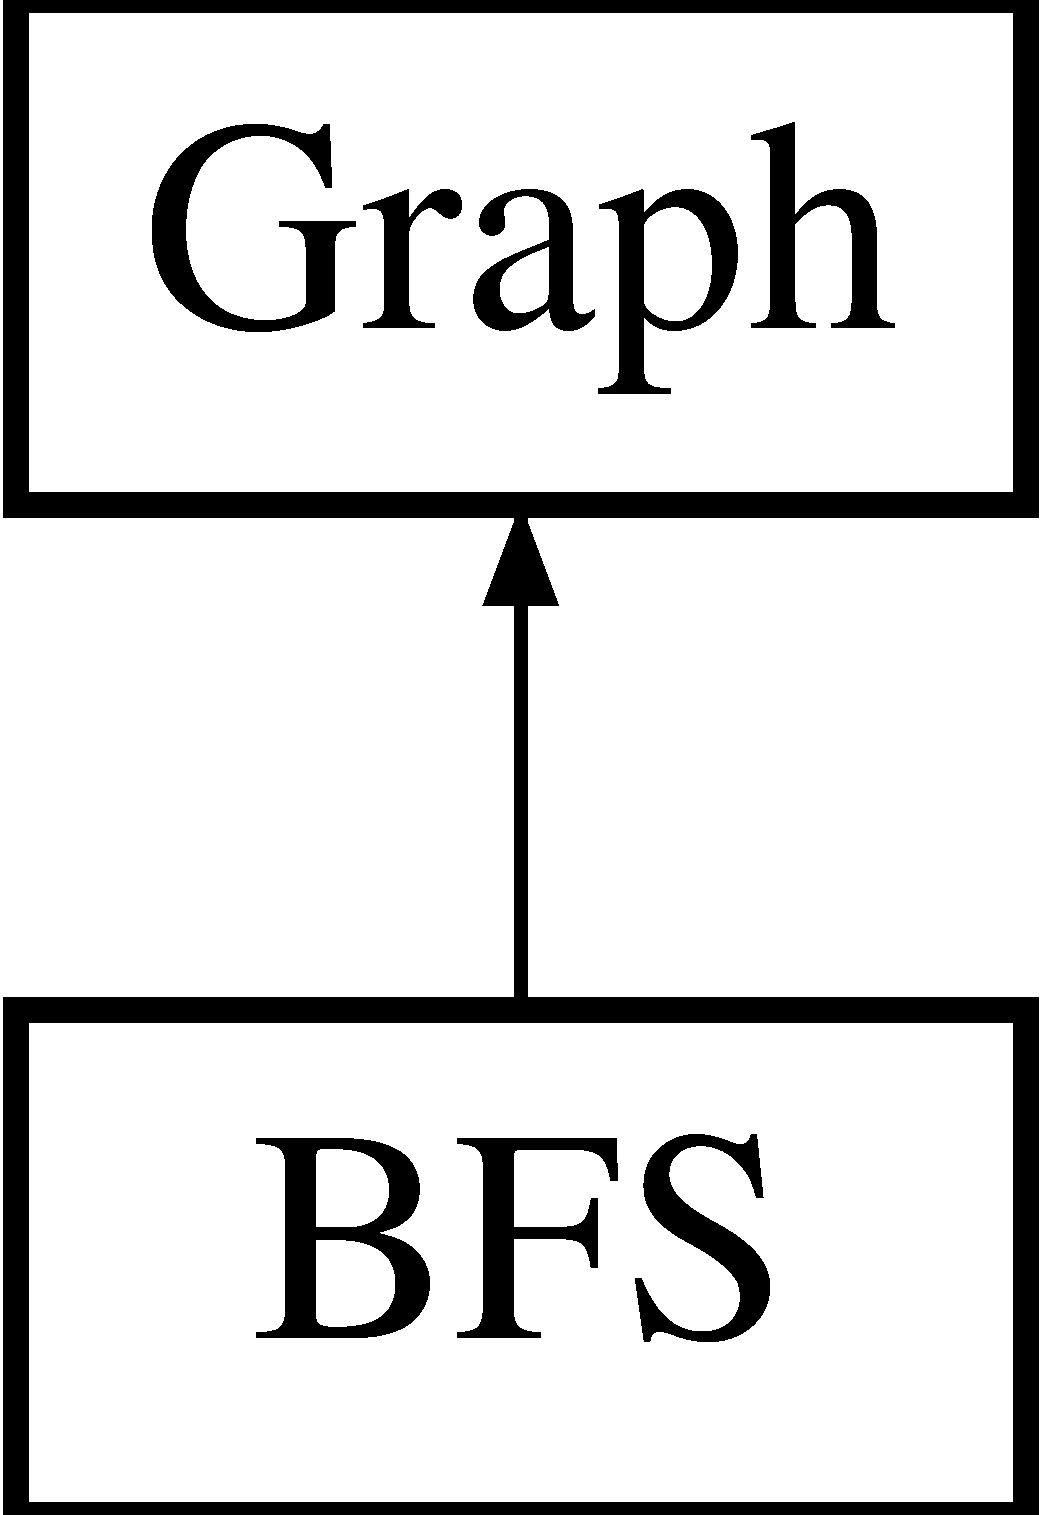
\includegraphics[height=2.000000cm]{class_b_f_s}
\end{center}
\end{figure}
\subsubsection*{Metody publiczne}
\begin{DoxyCompactItemize}
\item 
\hyperlink{class_b_f_s_ae2f1a5dc47c9791ad2d90e40e812d229}{B\-F\-S} ()
\begin{DoxyCompactList}\small\item\em Reprezentuje kolejnke elementów po wizycie. \end{DoxyCompactList}\item 
virtual \hyperlink{class_b_f_s_af70cee98b79886431c5d3f451d78f712}{$\sim$\-B\-F\-S} ()
\item 
void \hyperlink{class_b_f_s_a392b91df16399ab3be7e3745379d9dc0}{bfs} (int from\-Number, int to\-Number)
\item 
void \hyperlink{class_b_f_s_a42789813e256a0225a26cf418c7754a2}{find\-Shortest\-Path} (int from\-Number, int to\-Number)
\item 
void \hyperlink{class_b_f_s_a5d7b36488122996dc5877cd611afcaef}{clean} ()
\begin{DoxyCompactList}\small\item\em Zwalniam zasoby i przygotowuje do nowego rozruchu. \end{DoxyCompactList}\end{DoxyCompactItemize}
\subsubsection*{Atrybuty publiczne}
\begin{DoxyCompactItemize}
\item 
int \hyperlink{class_b_f_s_a1191eb3076bf8f3f412cc68563c0b46f}{pi} \mbox{[}\hyperlink{graph_8h_a392fb874e547e582e9c66a08a1f23326}{M\-A\-X}\mbox{]}
\item 
\hyperlink{class_linked_list}{Linked\-List}$<$ int $>$ \hyperlink{class_b_f_s_a317da6453a9b8e73f62e2bc60e9894fa}{q}
\begin{DoxyCompactList}\small\item\em rodzic nadego elementu \end{DoxyCompactList}\end{DoxyCompactItemize}


\subsubsection{Opis szczegółowy}


Definicja w linii \hyperlink{bfs_8h_source_l00018}{18} pliku \hyperlink{bfs_8h_source}{bfs.\-h}.



\subsubsection{Dokumentacja konstruktora i destruktora}
\hypertarget{class_b_f_s_ae2f1a5dc47c9791ad2d90e40e812d229}{\index{B\-F\-S@{B\-F\-S}!B\-F\-S@{B\-F\-S}}
\index{B\-F\-S@{B\-F\-S}!BFS@{B\-F\-S}}
\paragraph[{B\-F\-S}]{\setlength{\rightskip}{0pt plus 5cm}B\-F\-S\-::\-B\-F\-S (
\begin{DoxyParamCaption}
{}
\end{DoxyParamCaption}
)\hspace{0.3cm}{\ttfamily [inline]}}}\label{class_b_f_s_ae2f1a5dc47c9791ad2d90e40e812d229}


Definicja w linii \hyperlink{bfs_8h_source_l00024}{24} pliku \hyperlink{bfs_8h_source}{bfs.\-h}.


\begin{DoxyCode}
00025     \{
00026                 \hyperlink{class_b_f_s_a5d7b36488122996dc5877cd611afcaef}{clean}();
00027     \}
\end{DoxyCode}
\hypertarget{class_b_f_s_af70cee98b79886431c5d3f451d78f712}{\index{B\-F\-S@{B\-F\-S}!$\sim$\-B\-F\-S@{$\sim$\-B\-F\-S}}
\index{$\sim$\-B\-F\-S@{$\sim$\-B\-F\-S}!BFS@{B\-F\-S}}
\paragraph[{$\sim$\-B\-F\-S}]{\setlength{\rightskip}{0pt plus 5cm}virtual B\-F\-S\-::$\sim$\-B\-F\-S (
\begin{DoxyParamCaption}
{}
\end{DoxyParamCaption}
)\hspace{0.3cm}{\ttfamily [inline]}, {\ttfamily [virtual]}}}\label{class_b_f_s_af70cee98b79886431c5d3f451d78f712}


Definicja w linii \hyperlink{bfs_8h_source_l00028}{28} pliku \hyperlink{bfs_8h_source}{bfs.\-h}.


\begin{DoxyCode}
00028 \{        \}
\end{DoxyCode}


\subsubsection{Dokumentacja funkcji składowych}
\hypertarget{class_b_f_s_a392b91df16399ab3be7e3745379d9dc0}{\index{B\-F\-S@{B\-F\-S}!bfs@{bfs}}
\index{bfs@{bfs}!BFS@{B\-F\-S}}
\paragraph[{bfs}]{\setlength{\rightskip}{0pt plus 5cm}void B\-F\-S\-::bfs (
\begin{DoxyParamCaption}
\item[{int}]{from\-Number, }
\item[{int}]{to\-Number}
\end{DoxyParamCaption}
)\hspace{0.3cm}{\ttfamily [inline]}}}\label{class_b_f_s_a392b91df16399ab3be7e3745379d9dc0}


Definicja w linii \hyperlink{bfs_8h_source_l00030}{30} pliku \hyperlink{bfs_8h_source}{bfs.\-h}.


\begin{DoxyCode}
00031     \{
00032         \hyperlink{class_graph_aa13a7c7c066a77cc6dd21e4380deb649}{colour}[fromNumber] = 1;
00033         \hyperlink{class_b_f_s_a1191eb3076bf8f3f412cc68563c0b46f}{pi}[fromNumber]     = 1; \textcolor{comment}{// czyli brak rodzica}
00034         \hyperlink{class_b_f_s_a317da6453a9b8e73f62e2bc60e9894fa}{q}.\hyperlink{class_linked_list_a719c7b47925171fd7a72a35d0a581619}{push\_back}( fromNumber );
00035         \textcolor{keywordflow}{while} ( \hyperlink{class_b_f_s_a317da6453a9b8e73f62e2bc60e9894fa}{q}.\hyperlink{class_linked_list_ab399f1dc929c705e9cba628ae1f29254}{size}() ) \{
00036                 \textcolor{keywordtype}{int} u = \hyperlink{class_b_f_s_a317da6453a9b8e73f62e2bc60e9894fa}{q}[0];
00037                 \hyperlink{class_b_f_s_a317da6453a9b8e73f62e2bc60e9894fa}{q}.\hyperlink{class_linked_list_a64abea886f0dadf69a3726d1880c514a}{pop\_front}();
00038                 \textcolor{keywordflow}{for}( \textcolor{keywordtype}{int} v = 0; v < \hyperlink{class_graph_a73d1b5ba16c84f8eb1f6cf009b8ea532}{biggestValue}; v++ ) \{
00039                         \textcolor{comment}{//cout<<"(test) colour:"<<colour[v]<<"\(\backslash\)t"<<M[u][v]<<endl;}
00040                         \textcolor{keywordflow}{if}( \hyperlink{class_graph_aa13a7c7c066a77cc6dd21e4380deb649}{colour}[v] == 0 && \hyperlink{class_graph_ae948381c05ffc60825e5810328c0451c}{M}[u][v] ) \{
00041                                 \hyperlink{class_graph_aa13a7c7c066a77cc6dd21e4380deb649}{colour}[v] = 1;
00042                                 \hyperlink{class_b_f_s_a1191eb3076bf8f3f412cc68563c0b46f}{pi}[v] = u;         \textcolor{comment}{// zapisuje gdzie znajduje sie rodzic danej liczby}
00043                                 \textcolor{keywordflow}{if}(toNumber == v) \textcolor{keywordflow}{return};
00044                                 \hyperlink{class_b_f_s_a317da6453a9b8e73f62e2bc60e9894fa}{q}.\hyperlink{class_linked_list_a719c7b47925171fd7a72a35d0a581619}{push\_back}( v );
00045                         \}
00046                 \}
00047                 \hyperlink{class_graph_aa13a7c7c066a77cc6dd21e4380deb649}{colour}[u] = 2;
00048         \}
00049     \}
\end{DoxyCode}
\hypertarget{class_b_f_s_a5d7b36488122996dc5877cd611afcaef}{\index{B\-F\-S@{B\-F\-S}!clean@{clean}}
\index{clean@{clean}!BFS@{B\-F\-S}}
\paragraph[{clean}]{\setlength{\rightskip}{0pt plus 5cm}void B\-F\-S\-::clean (
\begin{DoxyParamCaption}
{}
\end{DoxyParamCaption}
)\hspace{0.3cm}{\ttfamily [inline]}, {\ttfamily [virtual]}}}\label{class_b_f_s_a5d7b36488122996dc5877cd611afcaef}


Implementuje \hyperlink{class_graph_a957781c55ace92dc6703b8d890b73ca7}{Graph}.



Definicja w linii \hyperlink{bfs_8h_source_l00068}{68} pliku \hyperlink{bfs_8h_source}{bfs.\-h}.



Odwołuje się do \hyperlink{bfs_8h_source_l00014}{M\-A\-X}.


\begin{DoxyCode}
00069     \{
00070         \hyperlink{class_graph_a895fee5bcf86093c8f57de9ed2304d8e}{num} = 0;
00071         \hyperlink{class_graph_a73d1b5ba16c84f8eb1f6cf009b8ea532}{biggestValue} = 0;
00072         \textcolor{keywordflow}{for} (\textcolor{keywordtype}{int} i = 0; i < \hyperlink{bfs_8h_a392fb874e547e582e9c66a08a1f23326}{MAX}; i++)
00073         \{
00074                 \textcolor{keywordflow}{for} (\textcolor{keywordtype}{int} j = 0; j < \hyperlink{bfs_8h_a392fb874e547e582e9c66a08a1f23326}{MAX}; j++)        \hyperlink{class_graph_ae948381c05ffc60825e5810328c0451c}{M}[i][j] = 0;
00075 
00076                 \hyperlink{class_graph_aa13a7c7c066a77cc6dd21e4380deb649}{colour}[i] = 0;    \textcolor{comment}{// ustawia numery jako biale}
00077                 \hyperlink{class_b_f_s_a1191eb3076bf8f3f412cc68563c0b46f}{pi}[i] = 1;   \textcolor{comment}{// ustawia rodzicow na 1}
00078 
00079         \}
00080     \}
\end{DoxyCode}
\hypertarget{class_b_f_s_a42789813e256a0225a26cf418c7754a2}{\index{B\-F\-S@{B\-F\-S}!find\-Shortest\-Path@{find\-Shortest\-Path}}
\index{find\-Shortest\-Path@{find\-Shortest\-Path}!BFS@{B\-F\-S}}
\paragraph[{find\-Shortest\-Path}]{\setlength{\rightskip}{0pt plus 5cm}void B\-F\-S\-::find\-Shortest\-Path (
\begin{DoxyParamCaption}
\item[{int}]{from\-Number, }
\item[{int}]{to\-Number}
\end{DoxyParamCaption}
)\hspace{0.3cm}{\ttfamily [inline]}, {\ttfamily [virtual]}}}\label{class_b_f_s_a42789813e256a0225a26cf418c7754a2}
najkrótszą drogę i wypusuje ją na ekran 
\begin{DoxyParams}{Parametry}
{\em from\-Number} & star poszukiwan \\
\hline
{\em end\-Number} & Koniec poszukiwan \\
\hline
\end{DoxyParams}


Implementuje \hyperlink{class_graph_adf2b7f7e78c0ac66f7f604021133561e}{Graph}.



Definicja w linii \hyperlink{bfs_8h_source_l00051}{51} pliku \hyperlink{bfs_8h_source}{bfs.\-h}.



Odwołuje się do \hyperlink{linkedlist_8h_source_l00144}{Linked\-List$<$ Content\-Type $>$\-::print()} i \hyperlink{linkedlist_8h_source_l00113}{Linked\-List$<$ Content\-Type $>$\-::push\-\_\-front()}.


\begin{DoxyCode}
00052     \{
00053         \hyperlink{class_linked_list}{LinkedList<int>} listaDoZmianyKolejnosci;
00054         \textcolor{keywordtype}{int} tmp=toNumber;
00055         \hyperlink{class_b_f_s_a392b91df16399ab3be7e3745379d9dc0}{bfs}(fromNumber, toNumber);
00056         listaDoZmianyKolejnosci.\hyperlink{class_linked_list_a9effa3698ad28e2f3401cd199f852e08}{push\_front}(toNumber);
00057         \textcolor{keywordflow}{while}(1)
00058         \{
00059                 listaDoZmianyKolejnosci.\hyperlink{class_linked_list_a9effa3698ad28e2f3401cd199f852e08}{push\_front}(\hyperlink{class_b_f_s_a1191eb3076bf8f3f412cc68563c0b46f}{pi}[tmp]);
00060                 tmp = \hyperlink{class_b_f_s_a1191eb3076bf8f3f412cc68563c0b46f}{pi}[tmp];
00061                 \textcolor{keywordflow}{if}(tmp == fromNumber) \textcolor{keywordflow}{break};
00062         \}
00063         listaDoZmianyKolejnosci.\hyperlink{class_linked_list_a245ba50906c85c1765a5f611d3f3b6c0}{print}();
00064     \}
\end{DoxyCode}


\subsubsection{Dokumentacja atrybutów składowych}
\hypertarget{class_b_f_s_a1191eb3076bf8f3f412cc68563c0b46f}{\index{B\-F\-S@{B\-F\-S}!pi@{pi}}
\index{pi@{pi}!BFS@{B\-F\-S}}
\paragraph[{pi}]{\setlength{\rightskip}{0pt plus 5cm}int B\-F\-S\-::pi\mbox{[}{\bf M\-A\-X}\mbox{]}}}\label{class_b_f_s_a1191eb3076bf8f3f412cc68563c0b46f}


Definicja w linii \hyperlink{bfs_8h_source_l00021}{21} pliku \hyperlink{bfs_8h_source}{bfs.\-h}.

\hypertarget{class_b_f_s_a317da6453a9b8e73f62e2bc60e9894fa}{\index{B\-F\-S@{B\-F\-S}!q@{q}}
\index{q@{q}!BFS@{B\-F\-S}}
\paragraph[{q}]{\setlength{\rightskip}{0pt plus 5cm}{\bf Linked\-List}$<$int$>$ B\-F\-S\-::q}}\label{class_b_f_s_a317da6453a9b8e73f62e2bc60e9894fa}


Definicja w linii \hyperlink{bfs_8h_source_l00022}{22} pliku \hyperlink{bfs_8h_source}{bfs.\-h}.



Dokumentacja dla tej klasy została wygenerowana z pliku\-:\begin{DoxyCompactItemize}
\item 
\hyperlink{bfs_8h}{bfs.\-h}\end{DoxyCompactItemize}

\hypertarget{class_d_f_s}{\subsection{Dokumentacja klasy D\-F\-S}
\label{class_d_f_s}\index{D\-F\-S@{D\-F\-S}}
}


Klasa przedstawia przeszukiwanie grafu za pomocą \hyperlink{class_d_f_s}{D\-F\-S} Umożliwia wyszukanie najkrótszej trasy do numeru.  




{\ttfamily \#include $<$dfs.\-h$>$}

Diagram dziedziczenia dla D\-F\-S\begin{figure}[H]
\begin{center}
\leavevmode
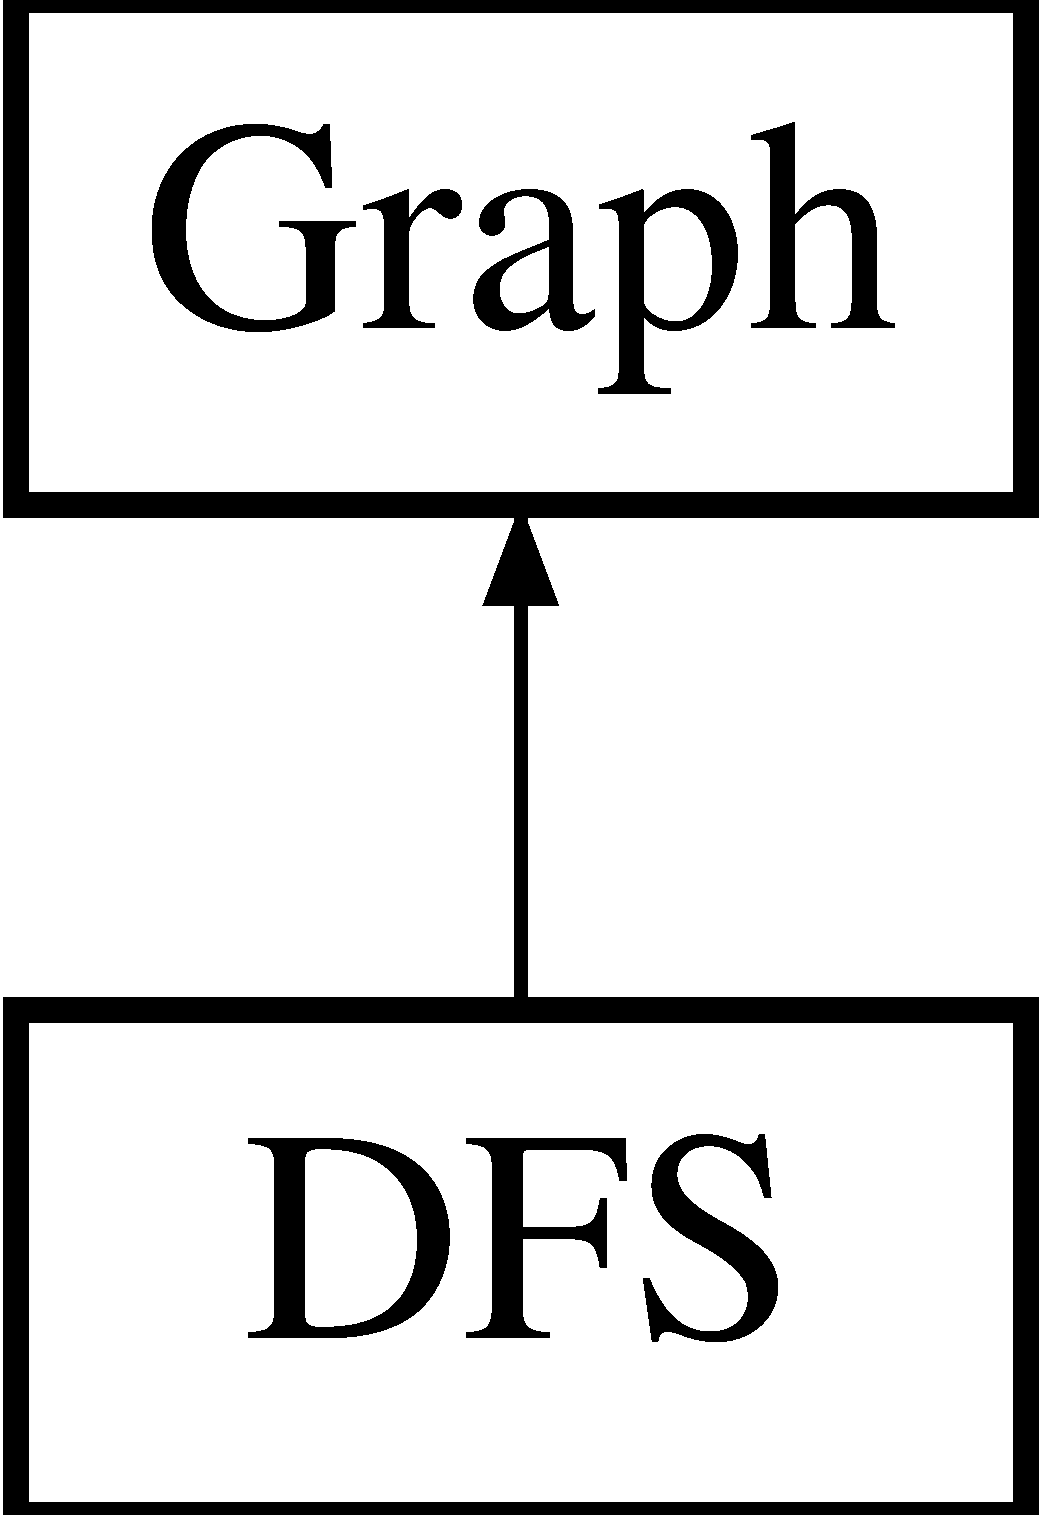
\includegraphics[height=2.000000cm]{class_d_f_s}
\end{center}
\end{figure}
\subsubsection*{Metody publiczne}
\begin{DoxyCompactItemize}
\item 
\hyperlink{class_d_f_s_a75b2f0e0042913c0a0a800e3d6c34f37}{D\-F\-S} ()
\begin{DoxyCompactList}\small\item\em wszystkich sciezek \end{DoxyCompactList}\item 
\hyperlink{class_d_f_s_aa013205788e77bad8ea56e138420c1ea}{$\sim$\-D\-F\-S} ()
\item 
void \hyperlink{class_d_f_s_a1d8f16ae45bf27ea6681236f5a4ba7f9}{find\-Path} (int u, int p, int searching\-Value)
\begin{DoxyCompactList}\small\item\em Znajduje wszystkie mozliwe sciezki do liczby. \end{DoxyCompactList}\item 
void \hyperlink{class_d_f_s_a7243745e5d6162b7106803ac1cd70d91}{find\-Shortest\-Path} (int from\-Number, int to\-Number)
\item 
void \hyperlink{class_d_f_s_ac335b86dce7cfab6655ca7eeaf2f9e10}{clean} ()
\begin{DoxyCompactList}\small\item\em Zwalniam zasoby i przygotowuje do nowego rozruchu. \end{DoxyCompactList}\end{DoxyCompactItemize}
\subsubsection*{Atrybuty publiczne}
\begin{DoxyCompactItemize}
\item 
\hyperlink{class_linked_list}{Linked\-List}$<$ int $>$ \hyperlink{class_d_f_s_aa3bf5c11cd2d66fc893e232eb1e42c76}{current\-Path}
\item 
\hyperlink{class_linked_list}{Linked\-List}$<$ int $>$ \hyperlink{class_d_f_s_a48dd546aaa57234bcd6e54a0f01b3f48}{all\-Paths} \mbox{[}\hyperlink{graph_8h_a392fb874e547e582e9c66a08a1f23326}{M\-A\-X}\mbox{]}
\begin{DoxyCompactList}\small\item\em znaleziona sciezka \end{DoxyCompactList}\item 
int \hyperlink{class_d_f_s_a53269340075995e432c355638ce30554}{all\-Paths\-Amount}
\begin{DoxyCompactList}\small\item\em wszystkich ścieżek do liczby \end{DoxyCompactList}\end{DoxyCompactItemize}


\subsubsection{Opis szczegółowy}


Definicja w linii \hyperlink{dfs_8h_source_l00022}{22} pliku \hyperlink{dfs_8h_source}{dfs.\-h}.



\subsubsection{Dokumentacja konstruktora i destruktora}
\hypertarget{class_d_f_s_a75b2f0e0042913c0a0a800e3d6c34f37}{\index{D\-F\-S@{D\-F\-S}!D\-F\-S@{D\-F\-S}}
\index{D\-F\-S@{D\-F\-S}!DFS@{D\-F\-S}}
\paragraph[{D\-F\-S}]{\setlength{\rightskip}{0pt plus 5cm}D\-F\-S\-::\-D\-F\-S (
\begin{DoxyParamCaption}
{}
\end{DoxyParamCaption}
)\hspace{0.3cm}{\ttfamily [inline]}}}\label{class_d_f_s_a75b2f0e0042913c0a0a800e3d6c34f37}


Definicja w linii \hyperlink{dfs_8h_source_l00029}{29} pliku \hyperlink{dfs_8h_source}{dfs.\-h}.


\begin{DoxyCode}
00030   \{
00031                 \hyperlink{class_d_f_s_ac335b86dce7cfab6655ca7eeaf2f9e10}{clean}();
00032   \}
\end{DoxyCode}
\hypertarget{class_d_f_s_aa013205788e77bad8ea56e138420c1ea}{\index{D\-F\-S@{D\-F\-S}!$\sim$\-D\-F\-S@{$\sim$\-D\-F\-S}}
\index{$\sim$\-D\-F\-S@{$\sim$\-D\-F\-S}!DFS@{D\-F\-S}}
\paragraph[{$\sim$\-D\-F\-S}]{\setlength{\rightskip}{0pt plus 5cm}D\-F\-S\-::$\sim$\-D\-F\-S (
\begin{DoxyParamCaption}
{}
\end{DoxyParamCaption}
)\hspace{0.3cm}{\ttfamily [inline]}}}\label{class_d_f_s_aa013205788e77bad8ea56e138420c1ea}


Definicja w linii \hyperlink{dfs_8h_source_l00033}{33} pliku \hyperlink{dfs_8h_source}{dfs.\-h}.


\begin{DoxyCode}
00033 \{        \}
\end{DoxyCode}


\subsubsection{Dokumentacja funkcji składowych}
\hypertarget{class_d_f_s_ac335b86dce7cfab6655ca7eeaf2f9e10}{\index{D\-F\-S@{D\-F\-S}!clean@{clean}}
\index{clean@{clean}!DFS@{D\-F\-S}}
\paragraph[{clean}]{\setlength{\rightskip}{0pt plus 5cm}void D\-F\-S\-::clean (
\begin{DoxyParamCaption}
{}
\end{DoxyParamCaption}
)\hspace{0.3cm}{\ttfamily [inline]}, {\ttfamily [virtual]}}}\label{class_d_f_s_ac335b86dce7cfab6655ca7eeaf2f9e10}


Implementuje \hyperlink{class_graph_a957781c55ace92dc6703b8d890b73ca7}{Graph}.



Definicja w linii \hyperlink{dfs_8h_source_l00096}{96} pliku \hyperlink{dfs_8h_source}{dfs.\-h}.



Odwołuje się do \hyperlink{dfs_8h_source_l00014}{M\-A\-X}.


\begin{DoxyCode}
00096                      \{
00097                 \textcolor{comment}{//n =0;}
00098                 \hyperlink{class_graph_a73d1b5ba16c84f8eb1f6cf009b8ea532}{biggestValue} = 0;
00099                 \textcolor{keywordflow}{for} (\textcolor{keywordtype}{int} i = 0; i < \hyperlink{dfs_8h_a392fb874e547e582e9c66a08a1f23326}{MAX}; i++)
00100                         \textcolor{keywordflow}{for} (\textcolor{keywordtype}{int} j = 0; j < \hyperlink{dfs_8h_a392fb874e547e582e9c66a08a1f23326}{MAX}; j++)
00101                                 \hyperlink{class_graph_ae948381c05ffc60825e5810328c0451c}{M}[i][j] = 0;
00102                 \textcolor{keywordflow}{for} (\textcolor{keywordtype}{int} i = 0; i < \hyperlink{dfs_8h_a392fb874e547e582e9c66a08a1f23326}{MAX}; i++) \{
00103                         \hyperlink{class_graph_aa13a7c7c066a77cc6dd21e4380deb649}{colour}[i] = 0;
00104                 \}
00105                 \hyperlink{class_graph_a895fee5bcf86093c8f57de9ed2304d8e}{num} = 0;
00106                 \hyperlink{class_d_f_s_a53269340075995e432c355638ce30554}{allPathsAmount} = 0;
00107         \}
\end{DoxyCode}
\hypertarget{class_d_f_s_a1d8f16ae45bf27ea6681236f5a4ba7f9}{\index{D\-F\-S@{D\-F\-S}!find\-Path@{find\-Path}}
\index{find\-Path@{find\-Path}!DFS@{D\-F\-S}}
\paragraph[{find\-Path}]{\setlength{\rightskip}{0pt plus 5cm}void D\-F\-S\-::find\-Path (
\begin{DoxyParamCaption}
\item[{int}]{u, }
\item[{int}]{p, }
\item[{int}]{searching\-Value}
\end{DoxyParamCaption}
)\hspace{0.3cm}{\ttfamily [inline]}}}\label{class_d_f_s_a1d8f16ae45bf27ea6681236f5a4ba7f9}

\begin{DoxyParams}{Parametry}
{\em u} & Od tej liczby zaczynam przeszukiwanie \\
\hline
{\em p} & Liczba rodzica \\
\hline
\end{DoxyParams}


Definicja w linii \hyperlink{dfs_8h_source_l00039}{39} pliku \hyperlink{dfs_8h_source}{dfs.\-h}.


\begin{DoxyCode}
00039                                                     \{
00040          \hyperlink{class_graph_aa13a7c7c066a77cc6dd21e4380deb649}{colour}[u] = 1;
00041          \textcolor{comment}{//cout<<u<<" zmieniam flage na szara\(\backslash\)n";}
00042          \hyperlink{class_d_f_s_aa3bf5c11cd2d66fc893e232eb1e42c76}{currentPath}.\hyperlink{class_linked_list_a719c7b47925171fd7a72a35d0a581619}{push\_back}(u);
00043          \textcolor{keywordflow}{if}(u == searchingValue)
00044                  \{
00045                          \textcolor{comment}{// Znalazlem TĄ LICZBE !!!}
00046                          \textcolor{comment}{// Dodaje teraz te liste do tablicy list wygranych allPaths}
00047                          \hyperlink{class_d_f_s_a48dd546aaa57234bcd6e54a0f01b3f48}{allPaths}[\hyperlink{class_d_f_s_a53269340075995e432c355638ce30554}{allPathsAmount}++].
      \hyperlink{class_list_a8a1ebc7ce83d77b83f58bd8c2ce2d683}{cloneFrom}(\hyperlink{class_d_f_s_aa3bf5c11cd2d66fc893e232eb1e42c76}{currentPath});
00048                         \hyperlink{class_graph_aa13a7c7c066a77cc6dd21e4380deb649}{colour}[u] = 0;
00049                          \textcolor{keywordflow}{return};
00050                  \}
00051 
00052          \hyperlink{class_graph_a895fee5bcf86093c8f57de9ed2304d8e}{num}++;
00053          \textcolor{keywordflow}{for}( \textcolor{keywordtype}{int} v = 0; v < \hyperlink{class_graph_a73d1b5ba16c84f8eb1f6cf009b8ea532}{biggestValue}; v++ ) \textcolor{keywordflow}{if}( \hyperlink{class_graph_ae948381c05ffc60825e5810328c0451c}{M}[u][v] && v != p )
00054          \{
00055              \textcolor{keywordflow}{if}( \hyperlink{class_graph_aa13a7c7c066a77cc6dd21e4380deb649}{colour}[v] == 0 ) \{
00056                  \textcolor{comment}{//cout<<u<<" -> "<<v<<"\(\backslash\)n";}
00057                  \hyperlink{class_d_f_s_a1d8f16ae45bf27ea6681236f5a4ba7f9}{findPath}( v, u , searchingValue);
00058              \}
00059              \textcolor{keywordflow}{else} \textcolor{keywordflow}{if}( \hyperlink{class_graph_aa13a7c7c066a77cc6dd21e4380deb649}{colour}[v] == 1 )
00060              \{
00061                  cout<<u<<\textcolor{stringliteral}{" znalazlem szare wiec sie cofam\(\backslash\)n"};
00062 
00063              \}
00064              \textcolor{keywordflow}{else}
00065              \{
00066                  cout<<u<<\textcolor{stringliteral}{" znalazlem czarne wiec sie cofam\(\backslash\)n"};
00067 
00068              \}
00069              \hyperlink{class_d_f_s_aa3bf5c11cd2d66fc893e232eb1e42c76}{currentPath}.\hyperlink{class_linked_list_ad7634e21b0ccd370906c4f28baaffa38}{pop\_back}();
00070          \}
00071          \textcolor{comment}{//zmieniam flage na czarna;}
00072          \hyperlink{class_graph_aa13a7c7c066a77cc6dd21e4380deb649}{colour}[u] = 0;
00073 
00074      \}
\end{DoxyCode}
\hypertarget{class_d_f_s_a7243745e5d6162b7106803ac1cd70d91}{\index{D\-F\-S@{D\-F\-S}!find\-Shortest\-Path@{find\-Shortest\-Path}}
\index{find\-Shortest\-Path@{find\-Shortest\-Path}!DFS@{D\-F\-S}}
\paragraph[{find\-Shortest\-Path}]{\setlength{\rightskip}{0pt plus 5cm}void D\-F\-S\-::find\-Shortest\-Path (
\begin{DoxyParamCaption}
\item[{int}]{from\-Number, }
\item[{int}]{to\-Number}
\end{DoxyParamCaption}
)\hspace{0.3cm}{\ttfamily [inline]}, {\ttfamily [virtual]}}}\label{class_d_f_s_a7243745e5d6162b7106803ac1cd70d91}
najkrótszą drogę i wypusuje ją na ekran 
\begin{DoxyParams}{Parametry}
{\em from\-Number} & star poszukiwan \\
\hline
{\em end\-Number} & Koniec poszukiwan \\
\hline
\end{DoxyParams}


Implementuje \hyperlink{class_graph_adf2b7f7e78c0ac66f7f604021133561e}{Graph}.



Definicja w linii \hyperlink{dfs_8h_source_l00080}{80} pliku \hyperlink{dfs_8h_source}{dfs.\-h}.


\begin{DoxyCode}
00081 \{
00082         \hyperlink{class_d_f_s_a1d8f16ae45bf27ea6681236f5a4ba7f9}{findPath}( fromNumber, -1 , toNumber);
00083         \textcolor{keywordtype}{int} indexOfSmallestList = 0;
00084 
00085         \textcolor{keywordflow}{for}(\textcolor{keywordtype}{int} i=0; i<\hyperlink{class_d_f_s_a53269340075995e432c355638ce30554}{allPathsAmount}; i++)
00086         \{
00087                 \textcolor{keywordflow}{if}( \hyperlink{class_d_f_s_a48dd546aaa57234bcd6e54a0f01b3f48}{allPaths}[indexOfSmallestList].size() >= \hyperlink{class_d_f_s_a48dd546aaa57234bcd6e54a0f01b3f48}{allPaths}[i].size() )
00088                 \{
00089                         indexOfSmallestList = i;
00090                 \}
00091         \}
00092         \hyperlink{class_d_f_s_a48dd546aaa57234bcd6e54a0f01b3f48}{allPaths}[indexOfSmallestList].\hyperlink{class_linked_list_a245ba50906c85c1765a5f611d3f3b6c0}{print}();
00093 \}
\end{DoxyCode}


\subsubsection{Dokumentacja atrybutów składowych}
\hypertarget{class_d_f_s_a48dd546aaa57234bcd6e54a0f01b3f48}{\index{D\-F\-S@{D\-F\-S}!all\-Paths@{all\-Paths}}
\index{all\-Paths@{all\-Paths}!DFS@{D\-F\-S}}
\paragraph[{all\-Paths}]{\setlength{\rightskip}{0pt plus 5cm}{\bf Linked\-List}$<$int$>$ D\-F\-S\-::all\-Paths\mbox{[}{\bf M\-A\-X}\mbox{]}}}\label{class_d_f_s_a48dd546aaa57234bcd6e54a0f01b3f48}


Definicja w linii \hyperlink{dfs_8h_source_l00026}{26} pliku \hyperlink{dfs_8h_source}{dfs.\-h}.

\hypertarget{class_d_f_s_a53269340075995e432c355638ce30554}{\index{D\-F\-S@{D\-F\-S}!all\-Paths\-Amount@{all\-Paths\-Amount}}
\index{all\-Paths\-Amount@{all\-Paths\-Amount}!DFS@{D\-F\-S}}
\paragraph[{all\-Paths\-Amount}]{\setlength{\rightskip}{0pt plus 5cm}int D\-F\-S\-::all\-Paths\-Amount}}\label{class_d_f_s_a53269340075995e432c355638ce30554}


Definicja w linii \hyperlink{dfs_8h_source_l00027}{27} pliku \hyperlink{dfs_8h_source}{dfs.\-h}.

\hypertarget{class_d_f_s_aa3bf5c11cd2d66fc893e232eb1e42c76}{\index{D\-F\-S@{D\-F\-S}!current\-Path@{current\-Path}}
\index{current\-Path@{current\-Path}!DFS@{D\-F\-S}}
\paragraph[{current\-Path}]{\setlength{\rightskip}{0pt plus 5cm}{\bf Linked\-List}$<$int$>$ D\-F\-S\-::current\-Path}}\label{class_d_f_s_aa3bf5c11cd2d66fc893e232eb1e42c76}


Definicja w linii \hyperlink{dfs_8h_source_l00025}{25} pliku \hyperlink{dfs_8h_source}{dfs.\-h}.



Dokumentacja dla tej klasy została wygenerowana z pliku\-:\begin{DoxyCompactItemize}
\item 
\hyperlink{dfs_8h}{dfs.\-h}\end{DoxyCompactItemize}

\hypertarget{class_graph}{\subsection{Dokumentacja klasy Graph}
\label{class_graph}\index{Graph@{Graph}}
}


{\ttfamily \#include $<$graph.\-h$>$}

Diagram dziedziczenia dla Graph\begin{figure}[H]
\begin{center}
\leavevmode
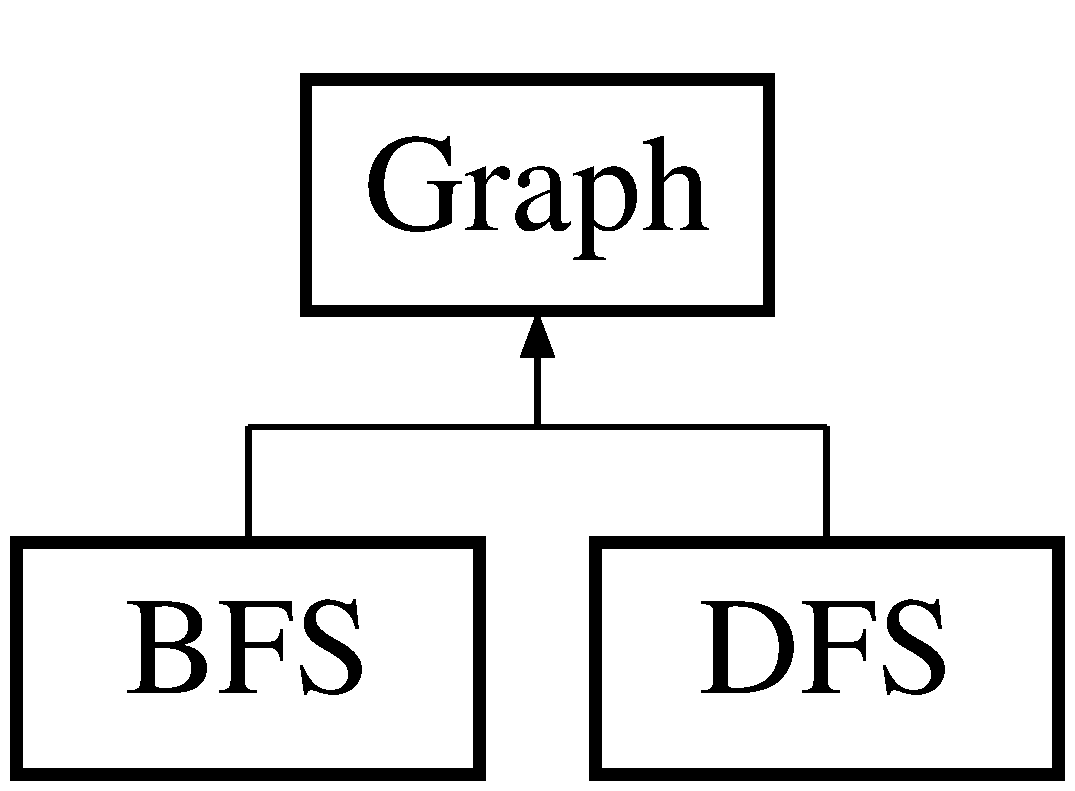
\includegraphics[height=2.000000cm]{class_graph}
\end{center}
\end{figure}
\subsubsection*{Metody publiczne}
\begin{DoxyCompactItemize}
\item 
virtual void \hyperlink{class_graph_adf2b7f7e78c0ac66f7f604021133561e}{find\-Shortest\-Path} (int from\-Number, int to\-Number)=0
\item 
virtual \hyperlink{class_graph_a1621cd1ffcf6a135cbc7e039c305627b}{$\sim$\-Graph} ()
\item 
void \hyperlink{class_graph_aca8b8f4b419f1495b6fe881e53811098}{add\-Edge} (int a, int b)
\item 
void \hyperlink{class_graph_a2ecf3dd3c4897aa924da8e5c221a8509}{print} ()
\begin{DoxyCompactList}\small\item\em Wyświetla graf. \end{DoxyCompactList}\item 
virtual void \hyperlink{class_graph_a957781c55ace92dc6703b8d890b73ca7}{clean} ()=0
\begin{DoxyCompactList}\small\item\em Zwalniam zasoby i przygotowuje do nowego rozruchu. \end{DoxyCompactList}\end{DoxyCompactItemize}
\subsubsection*{Atrybuty publiczne}
\begin{DoxyCompactItemize}
\item 
bool \hyperlink{class_graph_ae948381c05ffc60825e5810328c0451c}{M} \mbox{[}\hyperlink{graph_8h_a392fb874e547e582e9c66a08a1f23326}{M\-A\-X}\mbox{]}\mbox{[}\hyperlink{graph_8h_a392fb874e547e582e9c66a08a1f23326}{M\-A\-X}\mbox{]}
\item 
int \hyperlink{class_graph_aa13a7c7c066a77cc6dd21e4380deb649}{colour} \mbox{[}\hyperlink{graph_8h_a392fb874e547e582e9c66a08a1f23326}{M\-A\-X}\mbox{]}
\begin{DoxyCompactList}\small\item\em macierz numerów/indexów \end{DoxyCompactList}\item 
int \hyperlink{class_graph_a73d1b5ba16c84f8eb1f6cf009b8ea532}{biggest\-Value}
\begin{DoxyCompactList}\small\item\em tablica kolorów \end{DoxyCompactList}\item 
int \hyperlink{class_graph_a895fee5bcf86093c8f57de9ed2304d8e}{num}
\end{DoxyCompactItemize}


\subsubsection{Opis szczegółowy}


Definicja w linii \hyperlink{graph_8h_source_l00014}{14} pliku \hyperlink{graph_8h_source}{graph.\-h}.



\subsubsection{Dokumentacja konstruktora i destruktora}
\hypertarget{class_graph_a1621cd1ffcf6a135cbc7e039c305627b}{\index{Graph@{Graph}!$\sim$\-Graph@{$\sim$\-Graph}}
\index{$\sim$\-Graph@{$\sim$\-Graph}!Graph@{Graph}}
\paragraph[{$\sim$\-Graph}]{\setlength{\rightskip}{0pt plus 5cm}virtual Graph\-::$\sim$\-Graph (
\begin{DoxyParamCaption}
{}
\end{DoxyParamCaption}
)\hspace{0.3cm}{\ttfamily [inline]}, {\ttfamily [virtual]}}}\label{class_graph_a1621cd1ffcf6a135cbc7e039c305627b}


Definicja w linii \hyperlink{graph_8h_source_l00028}{28} pliku \hyperlink{graph_8h_source}{graph.\-h}.


\begin{DoxyCode}
00028 \{\}
\end{DoxyCode}


\subsubsection{Dokumentacja funkcji składowych}
\hypertarget{class_graph_aca8b8f4b419f1495b6fe881e53811098}{\index{Graph@{Graph}!add\-Edge@{add\-Edge}}
\index{add\-Edge@{add\-Edge}!Graph@{Graph}}
\paragraph[{add\-Edge}]{\setlength{\rightskip}{0pt plus 5cm}void Graph\-::add\-Edge (
\begin{DoxyParamCaption}
\item[{int}]{a, }
\item[{int}]{b}
\end{DoxyParamCaption}
)\hspace{0.3cm}{\ttfamily [inline]}}}\label{class_graph_aca8b8f4b419f1495b6fe881e53811098}
połączenia miedzy elementami

Dodaje je obustronne powiązenie między nimi aby łatwiej bylo potem generować dane do testowania 
\begin{DoxyParams}{Parametry}
{\em a} & jedna krawędz \\
\hline
{\em b} & druga krawędz \\
\hline
\end{DoxyParams}


Definicja w linii \hyperlink{graph_8h_source_l00036}{36} pliku \hyperlink{graph_8h_source}{graph.\-h}.



Odwołania w \hyperlink{main_8cpp_source_l00014}{main()}.


\begin{DoxyCode}
00037          \{
00038                   \hyperlink{class_graph_ae948381c05ffc60825e5810328c0451c}{M}[a][b] = 1;
00039                   \hyperlink{class_graph_ae948381c05ffc60825e5810328c0451c}{M}[b][a] = 1;
00040                   \textcolor{comment}{//n++;}
00041                   \textcolor{keywordflow}{if}(a>=\hyperlink{class_graph_a73d1b5ba16c84f8eb1f6cf009b8ea532}{biggestValue}) \hyperlink{class_graph_a73d1b5ba16c84f8eb1f6cf009b8ea532}{biggestValue}=a+1;
00042                   \textcolor{keywordflow}{if}(b>=\hyperlink{class_graph_a73d1b5ba16c84f8eb1f6cf009b8ea532}{biggestValue}) \hyperlink{class_graph_a73d1b5ba16c84f8eb1f6cf009b8ea532}{biggestValue}=b+1;
00043          \}
\end{DoxyCode}
\hypertarget{class_graph_a957781c55ace92dc6703b8d890b73ca7}{\index{Graph@{Graph}!clean@{clean}}
\index{clean@{clean}!Graph@{Graph}}
\paragraph[{clean}]{\setlength{\rightskip}{0pt plus 5cm}virtual void Graph\-::clean (
\begin{DoxyParamCaption}
{}
\end{DoxyParamCaption}
)\hspace{0.3cm}{\ttfamily [pure virtual]}}}\label{class_graph_a957781c55ace92dc6703b8d890b73ca7}


Implementowany w \hyperlink{class_d_f_s_ac335b86dce7cfab6655ca7eeaf2f9e10}{D\-F\-S} i \hyperlink{class_b_f_s_a5d7b36488122996dc5877cd611afcaef}{B\-F\-S}.



Odwołania w \hyperlink{main_8cpp_source_l00014}{main()}.

\hypertarget{class_graph_adf2b7f7e78c0ac66f7f604021133561e}{\index{Graph@{Graph}!find\-Shortest\-Path@{find\-Shortest\-Path}}
\index{find\-Shortest\-Path@{find\-Shortest\-Path}!Graph@{Graph}}
\paragraph[{find\-Shortest\-Path}]{\setlength{\rightskip}{0pt plus 5cm}virtual void Graph\-::find\-Shortest\-Path (
\begin{DoxyParamCaption}
\item[{int}]{from\-Number, }
\item[{int}]{to\-Number}
\end{DoxyParamCaption}
)\hspace{0.3cm}{\ttfamily [pure virtual]}}}\label{class_graph_adf2b7f7e78c0ac66f7f604021133561e}
najkrótszą drogę i wypusuje ją na ekran 
\begin{DoxyParams}{Parametry}
{\em from\-Number} & star poszukiwan \\
\hline
{\em end\-Number} & Koniec poszukiwan \\
\hline
\end{DoxyParams}


Implementowany w \hyperlink{class_d_f_s_a7243745e5d6162b7106803ac1cd70d91}{D\-F\-S} i \hyperlink{class_b_f_s_a42789813e256a0225a26cf418c7754a2}{B\-F\-S}.



Odwołania w \hyperlink{main_8cpp_source_l00014}{main()}.

\hypertarget{class_graph_a2ecf3dd3c4897aa924da8e5c221a8509}{\index{Graph@{Graph}!print@{print}}
\index{print@{print}!Graph@{Graph}}
\paragraph[{print}]{\setlength{\rightskip}{0pt plus 5cm}void Graph\-::print (
\begin{DoxyParamCaption}
{}
\end{DoxyParamCaption}
)\hspace{0.3cm}{\ttfamily [inline]}}}\label{class_graph_a2ecf3dd3c4897aa924da8e5c221a8509}


Definicja w linii \hyperlink{graph_8h_source_l00048}{48} pliku \hyperlink{graph_8h_source}{graph.\-h}.


\begin{DoxyCode}
00049           \{
00050                   cout<<\textcolor{stringliteral}{"\(\backslash\)t"};
00051                   \textcolor{keywordflow}{for}(\textcolor{keywordtype}{int} i=0; i<\hyperlink{class_graph_a73d1b5ba16c84f8eb1f6cf009b8ea532}{biggestValue}; i++) cout<<i<<\textcolor{stringliteral}{"\(\backslash\)t"};
00052                   cout<<\textcolor{stringliteral}{"\(\backslash\)n"};
00053                   \textcolor{keywordflow}{for}(\textcolor{keywordtype}{int} i=0; i<\hyperlink{class_graph_a73d1b5ba16c84f8eb1f6cf009b8ea532}{biggestValue}; i++)
00054                   \{
00055                           cout<<i<<\textcolor{stringliteral}{"\(\backslash\)t"};
00056                           \textcolor{keywordflow}{for}(\textcolor{keywordtype}{int} j=0; j<\hyperlink{class_graph_a73d1b5ba16c84f8eb1f6cf009b8ea532}{biggestValue}; j++)
00057                           \{
00058                                   cout<<\hyperlink{class_graph_ae948381c05ffc60825e5810328c0451c}{M}[i][j]<<\textcolor{stringliteral}{"\(\backslash\)t"};
00059                           \}
00060                           cout<<\textcolor{stringliteral}{"\(\backslash\)n"};
00061                   \}
00062           \}
\end{DoxyCode}


\subsubsection{Dokumentacja atrybutów składowych}
\hypertarget{class_graph_a73d1b5ba16c84f8eb1f6cf009b8ea532}{\index{Graph@{Graph}!biggest\-Value@{biggest\-Value}}
\index{biggest\-Value@{biggest\-Value}!Graph@{Graph}}
\paragraph[{biggest\-Value}]{\setlength{\rightskip}{0pt plus 5cm}int Graph\-::biggest\-Value}}\label{class_graph_a73d1b5ba16c84f8eb1f6cf009b8ea532}


Definicja w linii \hyperlink{graph_8h_source_l00019}{19} pliku \hyperlink{graph_8h_source}{graph.\-h}.

\hypertarget{class_graph_aa13a7c7c066a77cc6dd21e4380deb649}{\index{Graph@{Graph}!colour@{colour}}
\index{colour@{colour}!Graph@{Graph}}
\paragraph[{colour}]{\setlength{\rightskip}{0pt plus 5cm}int Graph\-::colour\mbox{[}{\bf M\-A\-X}\mbox{]}}}\label{class_graph_aa13a7c7c066a77cc6dd21e4380deb649}


Definicja w linii \hyperlink{graph_8h_source_l00018}{18} pliku \hyperlink{graph_8h_source}{graph.\-h}.

\hypertarget{class_graph_ae948381c05ffc60825e5810328c0451c}{\index{Graph@{Graph}!M@{M}}
\index{M@{M}!Graph@{Graph}}
\paragraph[{M}]{\setlength{\rightskip}{0pt plus 5cm}bool Graph\-::\-M\mbox{[}{\bf M\-A\-X}\mbox{]}\mbox{[}{\bf M\-A\-X}\mbox{]}}}\label{class_graph_ae948381c05ffc60825e5810328c0451c}


Definicja w linii \hyperlink{graph_8h_source_l00017}{17} pliku \hyperlink{graph_8h_source}{graph.\-h}.

\hypertarget{class_graph_a895fee5bcf86093c8f57de9ed2304d8e}{\index{Graph@{Graph}!num@{num}}
\index{num@{num}!Graph@{Graph}}
\paragraph[{num}]{\setlength{\rightskip}{0pt plus 5cm}int Graph\-::num}}\label{class_graph_a895fee5bcf86093c8f57de9ed2304d8e}


Definicja w linii \hyperlink{graph_8h_source_l00020}{20} pliku \hyperlink{graph_8h_source}{graph.\-h}.



Dokumentacja dla tej klasy została wygenerowana z pliku\-:\begin{DoxyCompactItemize}
\item 
\hyperlink{graph_8h}{graph.\-h}\end{DoxyCompactItemize}

\hypertarget{class_heap_sorter}{\subsection{Dokumentacja szablonu klasy Heap\-Sorter$<$ My\-List\-Element\-Type $>$}
\label{class_heap_sorter}\index{Heap\-Sorter$<$ My\-List\-Element\-Type $>$@{Heap\-Sorter$<$ My\-List\-Element\-Type $>$}}
}


Klasa sluzaca do obslugi sortowania przez kopcowanie.  




{\ttfamily \#include $<$heapsorter.\-h$>$}

Diagram dziedziczenia dla Heap\-Sorter$<$ My\-List\-Element\-Type $>$\begin{figure}[H]
\begin{center}
\leavevmode
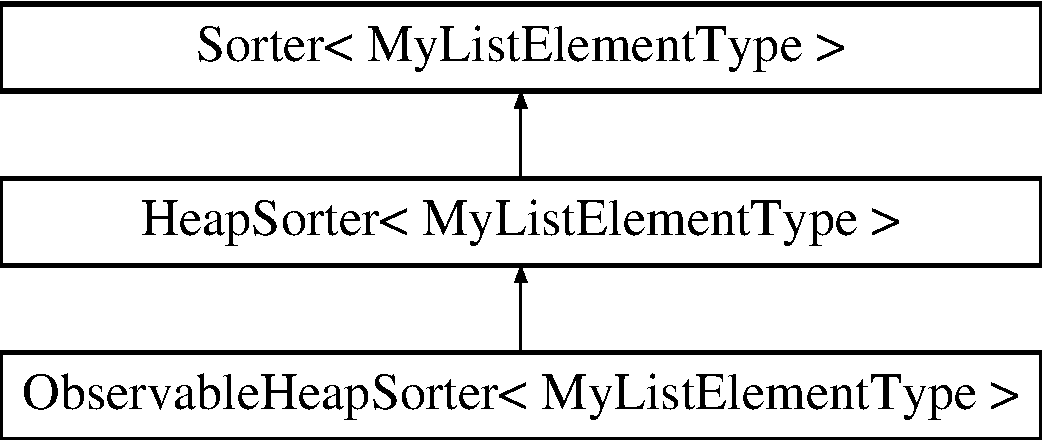
\includegraphics[height=3.000000cm]{class_heap_sorter}
\end{center}
\end{figure}
\subsubsection*{Metody publiczne}
\begin{DoxyCompactItemize}
\item 
\hyperlink{class_heap_sorter_a7d5fba788aae93bcfc1a300615dba080}{Heap\-Sorter} (\hyperlink{class_list}{List}$<$ My\-List\-Element\-Type $>$ \&my\-List)
\begin{DoxyCompactList}\small\item\em Konstruktor. \end{DoxyCompactList}\item 
virtual \hyperlink{class_heap_sorter_ab661e8598cf879b9c8f721c644633e66}{$\sim$\-Heap\-Sorter} ()
\item 
\hyperlink{class_list}{List}$<$ My\-List\-Element\-Type $>$ \& \hyperlink{class_heap_sorter_a31220ba55d4478c50578c3a94dcbf26c}{sort} ()
\begin{DoxyCompactList}\small\item\em Sortuje przez kopcowanie. \end{DoxyCompactList}\end{DoxyCompactItemize}
\subsubsection*{Atrybuty publiczne}
\begin{DoxyCompactItemize}
\item 
\hyperlink{class_list}{List}$<$ My\-List\-Element\-Type $>$ \& \hyperlink{class_heap_sorter_a6b8ac615ff2de0c2e510ad215d0508d9}{list}
\begin{DoxyCompactList}\small\item\em Skopiowana lista do przeprowadzania sortowania. \end{DoxyCompactList}\end{DoxyCompactItemize}


\subsubsection{Opis szczegółowy}
\subsubsection*{template$<$class My\-List\-Element\-Type$>$class Heap\-Sorter$<$ My\-List\-Element\-Type $>$}



Definicja w linii \hyperlink{heapsorter_8h_source_l00017}{17} pliku \hyperlink{heapsorter_8h_source}{heapsorter.\-h}.



\subsubsection{Dokumentacja konstruktora i destruktora}
\hypertarget{class_heap_sorter_a7d5fba788aae93bcfc1a300615dba080}{\index{Heap\-Sorter@{Heap\-Sorter}!Heap\-Sorter@{Heap\-Sorter}}
\index{Heap\-Sorter@{Heap\-Sorter}!HeapSorter@{Heap\-Sorter}}
\paragraph[{Heap\-Sorter}]{\setlength{\rightskip}{0pt plus 5cm}template$<$class My\-List\-Element\-Type $>$ {\bf Heap\-Sorter}$<$ My\-List\-Element\-Type $>$\-::{\bf Heap\-Sorter} (
\begin{DoxyParamCaption}
\item[{{\bf List}$<$ My\-List\-Element\-Type $>$ \&}]{my\-List}
\end{DoxyParamCaption}
)\hspace{0.3cm}{\ttfamily [inline]}}}\label{class_heap_sorter_a7d5fba788aae93bcfc1a300615dba080}

\begin{DoxyParams}{Parametry}
{\em \&my\-List} & lista, która konstruktor kopiuje aby nie naruszać podanej przez uzytkownika \\
\hline
\end{DoxyParams}


Definicja w linii \hyperlink{heapsorter_8h_source_l00026}{26} pliku \hyperlink{heapsorter_8h_source}{heapsorter.\-h}.



Odwołuje się do \hyperlink{heapsorter_8h_source_l00021}{Heap\-Sorter$<$ My\-List\-Element\-Type $>$\-::list}.


\begin{DoxyCode}
00027         :\hyperlink{class_heap_sorter_a6b8ac615ff2de0c2e510ad215d0508d9}{list}(myList.\hyperlink{class_list_a37f6551e13258a321c806fffb7e2f068}{createObjectFromAbstractReference}())
00028 
00029         \{
00030                 this->\hyperlink{class_heap_sorter_a6b8ac615ff2de0c2e510ad215d0508d9}{list}.cloneFrom(myList);
00031                 \textcolor{comment}{/*this->sizeOfList = myList.sizeOfList;}
00032 \textcolor{comment}{                this->firstElement = myList.firstElement;}
00033 \textcolor{comment}{                this->lastElement = myList.lastElement;}
00034 \textcolor{comment}{                this->iterator=myList.iterator;}
00035 \textcolor{comment}{                this->isIteratorAfterPop = myList.isIteratorAfterPop;*/}
00036         \}
\end{DoxyCode}
\hypertarget{class_heap_sorter_ab661e8598cf879b9c8f721c644633e66}{\index{Heap\-Sorter@{Heap\-Sorter}!$\sim$\-Heap\-Sorter@{$\sim$\-Heap\-Sorter}}
\index{$\sim$\-Heap\-Sorter@{$\sim$\-Heap\-Sorter}!HeapSorter@{Heap\-Sorter}}
\paragraph[{$\sim$\-Heap\-Sorter}]{\setlength{\rightskip}{0pt plus 5cm}template$<$class My\-List\-Element\-Type $>$ virtual {\bf Heap\-Sorter}$<$ My\-List\-Element\-Type $>$\-::$\sim${\bf Heap\-Sorter} (
\begin{DoxyParamCaption}
{}
\end{DoxyParamCaption}
)\hspace{0.3cm}{\ttfamily [inline]}, {\ttfamily [virtual]}}}\label{class_heap_sorter_ab661e8598cf879b9c8f721c644633e66}


Definicja w linii \hyperlink{heapsorter_8h_source_l00038}{38} pliku \hyperlink{heapsorter_8h_source}{heapsorter.\-h}.


\begin{DoxyCode}
00038 \{\};
\end{DoxyCode}


\subsubsection{Dokumentacja funkcji składowych}
\hypertarget{class_heap_sorter_a31220ba55d4478c50578c3a94dcbf26c}{\index{Heap\-Sorter@{Heap\-Sorter}!sort@{sort}}
\index{sort@{sort}!HeapSorter@{Heap\-Sorter}}
\paragraph[{sort}]{\setlength{\rightskip}{0pt plus 5cm}template$<$class My\-List\-Element\-Type $>$ {\bf List}$<$My\-List\-Element\-Type$>$\& {\bf Heap\-Sorter}$<$ My\-List\-Element\-Type $>$\-::sort (
\begin{DoxyParamCaption}
{}
\end{DoxyParamCaption}
)\hspace{0.3cm}{\ttfamily [inline]}, {\ttfamily [virtual]}}}\label{class_heap_sorter_a31220ba55d4478c50578c3a94dcbf26c}


Implementuje \hyperlink{class_sorter_a4a82d8151d6172802d1e60cb30c7d7d3}{Sorter$<$ My\-List\-Element\-Type $>$}.



Reimplementowana w \hyperlink{class_observable_heap_sorter_a5e92d70e5a769ba7249f974a48b94bd0}{Observable\-Heap\-Sorter$<$ My\-List\-Element\-Type $>$}.



Definicja w linii \hyperlink{heapsorter_8h_source_l00042}{42} pliku \hyperlink{heapsorter_8h_source}{heapsorter.\-h}.



Odwołuje się do \hyperlink{heapsorter_8h_source_l00021}{Heap\-Sorter$<$ My\-List\-Element\-Type $>$\-::list}.



Odwołania w \hyperlink{observableheapsorter_8h_source_l00026}{Observable\-Heap\-Sorter$<$ My\-List\-Element\-Type $>$\-::sort()}.


\begin{DoxyCode}
00043         \{
00044                 \textcolor{keywordtype}{int} n = this->\hyperlink{class_heap_sorter_a6b8ac615ff2de0c2e510ad215d0508d9}{list}.size();
00045             \textcolor{keywordtype}{int} parent = n/2, index, child, tmp; \textcolor{comment}{/* heap indexes */}
00046             \textcolor{comment}{/* czekam az sie posortuje */}
00047             \textcolor{keywordflow}{while} (1) \{
00048                 \textcolor{keywordflow}{if} (parent > 0)
00049                 \{
00050                     tmp = (this->\hyperlink{class_heap_sorter_a6b8ac615ff2de0c2e510ad215d0508d9}{list})[--parent].content;  \textcolor{comment}{/* kobie kopie do tmp */}
00051                 \}
00052                 \textcolor{keywordflow}{else} \{
00053                     n--;
00054                     \textcolor{keywordflow}{if} (n == 0)
00055                     \{
00056                         \textcolor{keywordflow}{return} this->\hyperlink{class_heap_sorter_a6b8ac615ff2de0c2e510ad215d0508d9}{list}; \textcolor{comment}{/* Zwraca posortowane */}
00057                     \}
00058                     tmp = this->\hyperlink{class_heap_sorter_a6b8ac615ff2de0c2e510ad215d0508d9}{list}[n].content;
00059                     this->\hyperlink{class_heap_sorter_a6b8ac615ff2de0c2e510ad215d0508d9}{list}[n].content = this->\hyperlink{class_heap_sorter_a6b8ac615ff2de0c2e510ad215d0508d9}{list}[0].content;
00060                 \}
00061                 index = parent;
00062                 child = index * 2 + 1;
00063                 \textcolor{keywordflow}{while} (child < n) \{
00064                     \textcolor{keywordflow}{if} (child + 1 < n  &&  this->\hyperlink{class_heap_sorter_a6b8ac615ff2de0c2e510ad215d0508d9}{list}[child + 1].content > this->
      \hyperlink{class_heap_sorter_a6b8ac615ff2de0c2e510ad215d0508d9}{list}[child].content) \{
00065                         child++;
00066                     \}
00067                     \textcolor{keywordflow}{if} (this->\hyperlink{class_heap_sorter_a6b8ac615ff2de0c2e510ad215d0508d9}{list}[child].content > tmp) \{
00068                         this->\hyperlink{class_heap_sorter_a6b8ac615ff2de0c2e510ad215d0508d9}{list}[index].content = this->\hyperlink{class_heap_sorter_a6b8ac615ff2de0c2e510ad215d0508d9}{list}[child].content;
00069                         index = child;
00070                         child = index * 2 + 1;
00071                     \} \textcolor{keywordflow}{else} \{
00072                         \textcolor{keywordflow}{break};
00073                     \}
00074                 \}
00075                 this->\hyperlink{class_heap_sorter_a6b8ac615ff2de0c2e510ad215d0508d9}{list}[index].content = tmp;
00076             \}
00077             \textcolor{keywordflow}{return} this->\hyperlink{class_heap_sorter_a6b8ac615ff2de0c2e510ad215d0508d9}{list};
00078         \}
\end{DoxyCode}


\subsubsection{Dokumentacja atrybutów składowych}
\hypertarget{class_heap_sorter_a6b8ac615ff2de0c2e510ad215d0508d9}{\index{Heap\-Sorter@{Heap\-Sorter}!list@{list}}
\index{list@{list}!HeapSorter@{Heap\-Sorter}}
\paragraph[{list}]{\setlength{\rightskip}{0pt plus 5cm}template$<$class My\-List\-Element\-Type $>$ {\bf List}$<$My\-List\-Element\-Type$>$\& {\bf Heap\-Sorter}$<$ My\-List\-Element\-Type $>$\-::list}}\label{class_heap_sorter_a6b8ac615ff2de0c2e510ad215d0508d9}


Definicja w linii \hyperlink{heapsorter_8h_source_l00021}{21} pliku \hyperlink{heapsorter_8h_source}{heapsorter.\-h}.



Odwołania w \hyperlink{heapsorter_8h_source_l00026}{Heap\-Sorter$<$ My\-List\-Element\-Type $>$\-::\-Heap\-Sorter()}, \hyperlink{main_8cpp_source_l00022}{main()}, \hyperlink{observableheapsorter_8h_source_l00026}{Observable\-Heap\-Sorter$<$ My\-List\-Element\-Type $>$\-::sort()} i \hyperlink{heapsorter_8h_source_l00042}{Heap\-Sorter$<$ My\-List\-Element\-Type $>$\-::sort()}.



Dokumentacja dla tej klasy została wygenerowana z pliku\-:\begin{DoxyCompactItemize}
\item 
\hyperlink{heapsorter_8h}{heapsorter.\-h}\end{DoxyCompactItemize}

\hypertarget{class_linked_list}{\subsection{Dokumentacja szablonu klasy Linked\-List$<$ Content\-Type $>$}
\label{class_linked_list}\index{Linked\-List$<$ Content\-Type $>$@{Linked\-List$<$ Content\-Type $>$}}
}


Lista dwukierunkowa.  




{\ttfamily \#include $<$linkedlist.\-h$>$}

Diagram dziedziczenia dla Linked\-List$<$ Content\-Type $>$\begin{figure}[H]
\begin{center}
\leavevmode
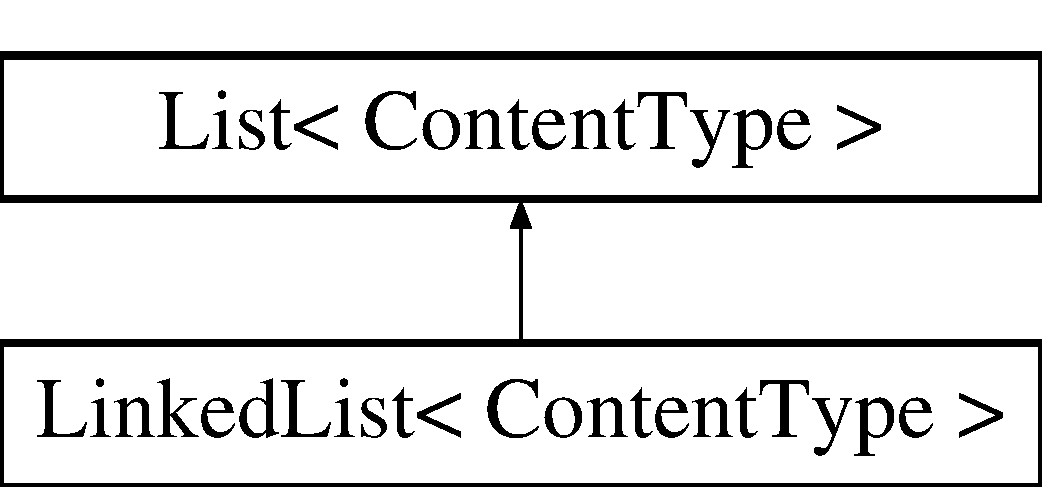
\includegraphics[height=2.000000cm]{class_linked_list}
\end{center}
\end{figure}
\subsubsection*{Metody publiczne}
\begin{DoxyCompactItemize}
\item 
\hyperlink{class_linked_list_a7528caae708f987831abf7ae722b5f18}{Linked\-List} ()
\begin{DoxyCompactList}\small\item\em Konstruktor listy. \end{DoxyCompactList}\item 
\hyperlink{class_linked_list_a9819b4a94bea2ee29f424ae3192a0078}{Linked\-List} (\hyperlink{class_list}{List}$<$ Content\-Type $>$ \&list)
\item 
virtual \hyperlink{class_linked_list_ae0e04b65a2b2327a53db60fe2957063b}{$\sim$\-Linked\-List} ()
\item 
int \& \hyperlink{class_linked_list_ab399f1dc929c705e9cba628ae1f29254}{size} ()
\begin{DoxyCompactList}\small\item\em Zwraca ilosc elementow listy. \end{DoxyCompactList}\item 
Content\-Type \hyperlink{class_linked_list_ad7634e21b0ccd370906c4f28baaffa38}{pop\-\_\-back} ()
\begin{DoxyCompactList}\small\item\em Zwraca element ostatni w liscie. \end{DoxyCompactList}\item 
Content\-Type \hyperlink{class_linked_list_a64abea886f0dadf69a3726d1880c514a}{pop\-\_\-front} ()
\begin{DoxyCompactList}\small\item\em Zwraca element pierwszy w liscie. \end{DoxyCompactList}\item 
void \hyperlink{class_linked_list_a719c7b47925171fd7a72a35d0a581619}{push\-\_\-back} (Content\-Type \&arg)
\begin{DoxyCompactList}\small\item\em Wklada element na ostatnie miejsce na liscie. \end{DoxyCompactList}\item 
void \hyperlink{class_linked_list_a9effa3698ad28e2f3401cd199f852e08}{push\-\_\-front} (Content\-Type \&arg)
\begin{DoxyCompactList}\small\item\em Wklada element na pierwsze miejsce na liscie. \end{DoxyCompactList}\item 
Content\-Type \& \hyperlink{class_linked_list_a2dcb9f488e5d179e89283a3f499acb76}{show\-\_\-front} ()
\begin{DoxyCompactList}\small\item\em Pokazuje element po poczatku listy. \end{DoxyCompactList}\item 
Content\-Type \& \hyperlink{class_linked_list_a437b5a0b96ab11f75e0391c76770186a}{show\-\_\-back} ()
\begin{DoxyCompactList}\small\item\em Pokazuje element po koncu listy. \end{DoxyCompactList}\item 
void \hyperlink{class_linked_list_a245ba50906c85c1765a5f611d3f3b6c0}{print} ()
\begin{DoxyCompactList}\small\item\em Wyswietla elementy listy. \end{DoxyCompactList}\item 
Content\-Type \& \hyperlink{class_linked_list_ad99e35cef5826d1cd456713ff8358a86}{operator\mbox{[}$\,$\mbox{]}} (int number\-Of\-Element)
\begin{DoxyCompactList}\small\item\em Pobiera element z listy. \end{DoxyCompactList}\item 
\hyperlink{class_linked_list_element}{Linked\-List\-Element}$<$ Content\-Type $>$ \& \hyperlink{class_linked_list_a32febc46a989c7af9bf8043da069e7df}{get\-Linked\-List\-Element\-By\-Id} (int number\-Of\-Element)
\item 
void \hyperlink{class_linked_list_aa882477023311c1400a724edd415e362}{insert\-After} (Content\-Type \&arg, int iterator\-I\-D)
\begin{DoxyCompactList}\small\item\em Wsadza element po obiekcie iteratora. \end{DoxyCompactList}\item 
\hyperlink{class_linked_list}{Linked\-List}$<$ Content\-Type $>$ \& \hyperlink{class_linked_list_a0dc224aa9930d4cbd80ecbd15c12b6d3}{operator=} (const \hyperlink{class_linked_list}{Linked\-List}$<$ Content\-Type $>$ \&pattern)
\item 
\hyperlink{class_list}{List}$<$ Content\-Type $>$ \& \hyperlink{class_linked_list_aea53fafbbe620165ec3173ad3566785d}{create\-Object\-From\-Abstract\-Reference} ()
\begin{DoxyCompactList}\small\item\em Wzorzec projektowy -\/ fabryki abstrakcyjnej. \end{DoxyCompactList}\end{DoxyCompactItemize}
\subsubsection*{Atrybuty publiczne}
\begin{DoxyCompactItemize}
\item 
int \hyperlink{class_linked_list_acfd83fe531d962d6260a633dfca98a9f}{size\-Of\-List}
\begin{DoxyCompactList}\small\item\em liczba elementow listy \end{DoxyCompactList}\item 
\hyperlink{class_linked_list_element}{Linked\-List\-Element}$<$ Content\-Type $>$ $\ast$ \hyperlink{class_linked_list_a51c0816c49528a63eea2adae2d503ada}{first\-Element}
\begin{DoxyCompactList}\small\item\em wskaznik do 'malej struktury' ktora jest pierwsza na liscie \end{DoxyCompactList}\item 
\hyperlink{class_linked_list_element}{Linked\-List\-Element}$<$ Content\-Type $>$ $\ast$ \hyperlink{class_linked_list_a8ca0cc6c38131c17f1626bb04a472fc9}{last\-Element}
\begin{DoxyCompactList}\small\item\em wskaznik do 'malej struktury' ktora jest ostatnia na liscie \end{DoxyCompactList}\item 
\hyperlink{class_linked_list_element}{Linked\-List\-Element}$<$ Content\-Type $>$ $\ast$ \hyperlink{class_linked_list_a6f117a991b3e2e020f43807500b45f5f}{iterator}
\item 
int \hyperlink{class_linked_list_a6398cec56a986426925e4e651bc4725c}{iterator\-Element\-Id}
\item 
int \hyperlink{class_linked_list_a8d354ba516e8270027bf617b121b49fe}{is\-Iterator\-After\-Pop}
\end{DoxyCompactItemize}


\subsubsection{Opis szczegółowy}
\subsubsection*{template$<$class Content\-Type$>$class Linked\-List$<$ Content\-Type $>$}

Klasa przedstawia liste dwukierunkową dynamiczna 

Definicja w linii \hyperlink{linkedlist_8h_source_l00022}{22} pliku \hyperlink{linkedlist_8h_source}{linkedlist.\-h}.



\subsubsection{Dokumentacja konstruktora i destruktora}
\hypertarget{class_linked_list_a7528caae708f987831abf7ae722b5f18}{\index{Linked\-List@{Linked\-List}!Linked\-List@{Linked\-List}}
\index{Linked\-List@{Linked\-List}!LinkedList@{Linked\-List}}
\paragraph[{Linked\-List}]{\setlength{\rightskip}{0pt plus 5cm}template$<$class Content\-Type$>$ {\bf Linked\-List}$<$ Content\-Type $>$\-::{\bf Linked\-List} (
\begin{DoxyParamCaption}
{}
\end{DoxyParamCaption}
)\hspace{0.3cm}{\ttfamily [inline]}}}\label{class_linked_list_a7528caae708f987831abf7ae722b5f18}


Definicja w linii \hyperlink{linkedlist_8h_source_l00038}{38} pliku \hyperlink{linkedlist_8h_source}{linkedlist.\-h}.


\begin{DoxyCode}
00039         \{
00040                 \hyperlink{class_linked_list_a51c0816c49528a63eea2adae2d503ada}{firstElement} = \hyperlink{class_linked_list_a8ca0cc6c38131c17f1626bb04a472fc9}{lastElement} = \textcolor{keyword}{new} 
      \hyperlink{class_linked_list_element}{LinkedListElement<ContentType>};
00041                 \hyperlink{class_linked_list_acfd83fe531d962d6260a633dfca98a9f}{sizeOfList} = 0;
00042                 \hyperlink{class_linked_list_a6398cec56a986426925e4e651bc4725c}{iteratorElementId} =0;
00043                 \hyperlink{class_linked_list_a6f117a991b3e2e020f43807500b45f5f}{iterator}=NULL;
00044                 \hyperlink{class_linked_list_a8d354ba516e8270027bf617b121b49fe}{isIteratorAfterPop} = 1; \textcolor{comment}{//to znaczy ze jeszcze raz trzeba bedzie
       sprawdzic pozycje iteratora 1- znaczy ze trzeba sprawdzic}
00045         \}
\end{DoxyCode}
\hypertarget{class_linked_list_a9819b4a94bea2ee29f424ae3192a0078}{\index{Linked\-List@{Linked\-List}!Linked\-List@{Linked\-List}}
\index{Linked\-List@{Linked\-List}!LinkedList@{Linked\-List}}
\paragraph[{Linked\-List}]{\setlength{\rightskip}{0pt plus 5cm}template$<$class Content\-Type$>$ {\bf Linked\-List}$<$ Content\-Type $>$\-::{\bf Linked\-List} (
\begin{DoxyParamCaption}
\item[{{\bf List}$<$ Content\-Type $>$ \&}]{list}
\end{DoxyParamCaption}
)\hspace{0.3cm}{\ttfamily [inline]}}}\label{class_linked_list_a9819b4a94bea2ee29f424ae3192a0078}


Definicja w linii \hyperlink{linkedlist_8h_source_l00047}{47} pliku \hyperlink{linkedlist_8h_source}{linkedlist.\-h}.


\begin{DoxyCode}
00048         \{
00049                 \hyperlink{class_linked_list_a51c0816c49528a63eea2adae2d503ada}{firstElement} = \hyperlink{class_linked_list_a8ca0cc6c38131c17f1626bb04a472fc9}{lastElement} = \textcolor{keyword}{new} 
      \hyperlink{class_linked_list_element}{LinkedListElement<ContentType>};
00050                 \hyperlink{class_linked_list_acfd83fe531d962d6260a633dfca98a9f}{sizeOfList} = 0;
00051                 \hyperlink{class_linked_list_a6398cec56a986426925e4e651bc4725c}{iteratorElementId} =0;
00052                 \hyperlink{class_linked_list_a6f117a991b3e2e020f43807500b45f5f}{iterator}=NULL;
00053                 \hyperlink{class_linked_list_a8d354ba516e8270027bf617b121b49fe}{isIteratorAfterPop} = 1; \textcolor{comment}{//to znaczy ze jeszcze raz trzeba bedzie
       sprawdzic pozycje iteratora 1- znaczy ze trzeba sprawdzic}
00054                 \textcolor{keywordflow}{for}(\textcolor{keywordtype}{int} i=0; i<list.\hyperlink{class_list_a61bc4a0a8a2103d503f88b79d758f271}{size}(); i++)
00055                 \{
00056                         this->\hyperlink{class_linked_list_a719c7b47925171fd7a72a35d0a581619}{push\_back}(list[i]);
00057                 \}
00058         \}
\end{DoxyCode}
\hypertarget{class_linked_list_ae0e04b65a2b2327a53db60fe2957063b}{\index{Linked\-List@{Linked\-List}!$\sim$\-Linked\-List@{$\sim$\-Linked\-List}}
\index{$\sim$\-Linked\-List@{$\sim$\-Linked\-List}!LinkedList@{Linked\-List}}
\paragraph[{$\sim$\-Linked\-List}]{\setlength{\rightskip}{0pt plus 5cm}template$<$class Content\-Type$>$ virtual {\bf Linked\-List}$<$ Content\-Type $>$\-::$\sim${\bf Linked\-List} (
\begin{DoxyParamCaption}
{}
\end{DoxyParamCaption}
)\hspace{0.3cm}{\ttfamily [inline]}, {\ttfamily [virtual]}}}\label{class_linked_list_ae0e04b65a2b2327a53db60fe2957063b}


Definicja w linii \hyperlink{linkedlist_8h_source_l00059}{59} pliku \hyperlink{linkedlist_8h_source}{linkedlist.\-h}.


\begin{DoxyCode}
00059 \{\};
\end{DoxyCode}


\subsubsection{Dokumentacja funkcji składowych}
\hypertarget{class_linked_list_aea53fafbbe620165ec3173ad3566785d}{\index{Linked\-List@{Linked\-List}!create\-Object\-From\-Abstract\-Reference@{create\-Object\-From\-Abstract\-Reference}}
\index{create\-Object\-From\-Abstract\-Reference@{create\-Object\-From\-Abstract\-Reference}!LinkedList@{Linked\-List}}
\paragraph[{create\-Object\-From\-Abstract\-Reference}]{\setlength{\rightskip}{0pt plus 5cm}template$<$class Content\-Type$>$ {\bf List}$<$Content\-Type$>$\& {\bf Linked\-List}$<$ Content\-Type $>$\-::create\-Object\-From\-Abstract\-Reference (
\begin{DoxyParamCaption}
{}
\end{DoxyParamCaption}
)\hspace{0.3cm}{\ttfamily [inline]}, {\ttfamily [virtual]}}}\label{class_linked_list_aea53fafbbe620165ec3173ad3566785d}


Implementuje \hyperlink{class_list_a87870a63c8d7bb7530356d9278e766a9}{List$<$ Content\-Type $>$}.



Definicja w linii \hyperlink{linkedlist_8h_source_l00295}{295} pliku \hyperlink{linkedlist_8h_source}{linkedlist.\-h}.


\begin{DoxyCode}
00296         \{
00297                 \textcolor{keywordflow}{return} *\textcolor{keyword}{new} \hyperlink{class_linked_list}{LinkedList<ContentType>};
00298         \}
\end{DoxyCode}
\hypertarget{class_linked_list_a32febc46a989c7af9bf8043da069e7df}{\index{Linked\-List@{Linked\-List}!get\-Linked\-List\-Element\-By\-Id@{get\-Linked\-List\-Element\-By\-Id}}
\index{get\-Linked\-List\-Element\-By\-Id@{get\-Linked\-List\-Element\-By\-Id}!LinkedList@{Linked\-List}}
\paragraph[{get\-Linked\-List\-Element\-By\-Id}]{\setlength{\rightskip}{0pt plus 5cm}template$<$class Content\-Type$>$ {\bf Linked\-List\-Element}$<$Content\-Type$>$\& {\bf Linked\-List}$<$ Content\-Type $>$\-::get\-Linked\-List\-Element\-By\-Id (
\begin{DoxyParamCaption}
\item[{int}]{number\-Of\-Element}
\end{DoxyParamCaption}
)\hspace{0.3cm}{\ttfamily [inline]}}}\label{class_linked_list_a32febc46a989c7af9bf8043da069e7df}


Definicja w linii \hyperlink{linkedlist_8h_source_l00197}{197} pliku \hyperlink{linkedlist_8h_source}{linkedlist.\-h}.


\begin{DoxyCode}
00198         \{
00199                 \textcolor{comment}{//std::cerr<<"\(\backslash\)nJestem w ["<<numberOfElement<<"] iterator="<<iteratorElementId;}
00200                 \textcolor{keywordflow}{if}(numberOfElement > (\hyperlink{class_linked_list_acfd83fe531d962d6260a633dfca98a9f}{sizeOfList}-1)) \textcolor{comment}{// jezeli wyszedlem poza liste}
00201                         \{
00202                                 std::cerr<<\textcolor{stringliteral}{"\(\backslash\)n! Error indeks o numerze: "}<<numberOfElement<<\textcolor{stringliteral}{" nie istnieje
       !"};
00203                                 \textcolor{keywordflow}{return} *\hyperlink{class_linked_list_a6f117a991b3e2e020f43807500b45f5f}{iterator};
00204                         \}
00205                 \textcolor{keywordflow}{if}(\hyperlink{class_linked_list_a8d354ba516e8270027bf617b121b49fe}{isIteratorAfterPop})
00206                         \{
00207                                 \hyperlink{class_linked_list_a6398cec56a986426925e4e651bc4725c}{iteratorElementId}=0;  \textcolor{comment}{// czyli iterator byl zpopowany}
00208                                 \hyperlink{class_linked_list_a6f117a991b3e2e020f43807500b45f5f}{iterator} = \hyperlink{class_linked_list_a51c0816c49528a63eea2adae2d503ada}{firstElement};
00209                                 \hyperlink{class_linked_list_a8d354ba516e8270027bf617b121b49fe}{isIteratorAfterPop}=0;
00210                         \}
00211                 \textcolor{comment}{//std::cerr<<"\(\backslash\)nsprawdzam w ["<<numberOfElement<<"] iterator="<<iteratorElementId;}
00212                 \textcolor{keywordflow}{if}((numberOfElement <= \hyperlink{class_linked_list_a6398cec56a986426925e4e651bc4725c}{iteratorElementId}-numberOfElement) &&(
      \hyperlink{class_linked_list_a6398cec56a986426925e4e651bc4725c}{iteratorElementId}-numberOfElement>=0))
00213                 \{
00214                         \textcolor{comment}{//std::cerr<<"\(\backslash\)nJestem w if\_1";}
00215                         \hyperlink{class_linked_list_a6f117a991b3e2e020f43807500b45f5f}{iterator} = (this->\hyperlink{class_linked_list_a51c0816c49528a63eea2adae2d503ada}{firstElement});
00216                         \hyperlink{class_linked_list_a6398cec56a986426925e4e651bc4725c}{iteratorElementId} = 0;
00217                         \textcolor{keywordflow}{for} (; \hyperlink{class_linked_list_a6398cec56a986426925e4e651bc4725c}{iteratorElementId}< numberOfElement ; 
      \hyperlink{class_linked_list_a6398cec56a986426925e4e651bc4725c}{iteratorElementId}++)
00218                                 \hyperlink{class_linked_list_a6f117a991b3e2e020f43807500b45f5f}{iterator} = (\hyperlink{class_linked_list_a6f117a991b3e2e020f43807500b45f5f}{iterator}->nextElement);
00219                 \}
00220                 \textcolor{keywordflow}{else} \textcolor{keywordflow}{if}(numberOfElement > \hyperlink{class_linked_list_a6398cec56a986426925e4e651bc4725c}{iteratorElementId})
00221                 \{
00222                         \textcolor{comment}{//std::cerr<<"\(\backslash\)nJestem w if\_2";}
00223                         \textcolor{keywordflow}{for} (; \hyperlink{class_linked_list_a6398cec56a986426925e4e651bc4725c}{iteratorElementId}< numberOfElement ; 
      \hyperlink{class_linked_list_a6398cec56a986426925e4e651bc4725c}{iteratorElementId}++)
00224                                                 \hyperlink{class_linked_list_a6f117a991b3e2e020f43807500b45f5f}{iterator} = (\hyperlink{class_linked_list_a6f117a991b3e2e020f43807500b45f5f}{iterator}->nextElement);
00225                 \}
00226                 \textcolor{keywordflow}{else} \textcolor{keywordflow}{if}( numberOfElement < \hyperlink{class_linked_list_a6398cec56a986426925e4e651bc4725c}{iteratorElementId})
00227                 \{
00228                         \textcolor{comment}{//std::cerr<<"\(\backslash\)nJestem w if\_3";}
00229                         \textcolor{keywordflow}{for} (; \hyperlink{class_linked_list_a6398cec56a986426925e4e651bc4725c}{iteratorElementId}> numberOfElement ; 
      \hyperlink{class_linked_list_a6398cec56a986426925e4e651bc4725c}{iteratorElementId}--)
00230                                                 \hyperlink{class_linked_list_a6f117a991b3e2e020f43807500b45f5f}{iterator} = (\hyperlink{class_linked_list_a6f117a991b3e2e020f43807500b45f5f}{iterator}->previousElement);
00231                 \}
00232                 \textcolor{keywordflow}{return} *\hyperlink{class_linked_list_a6f117a991b3e2e020f43807500b45f5f}{iterator};
00233         \}
\end{DoxyCode}
\hypertarget{class_linked_list_aa882477023311c1400a724edd415e362}{\index{Linked\-List@{Linked\-List}!insert\-After@{insert\-After}}
\index{insert\-After@{insert\-After}!LinkedList@{Linked\-List}}
\paragraph[{insert\-After}]{\setlength{\rightskip}{0pt plus 5cm}template$<$class Content\-Type$>$ void {\bf Linked\-List}$<$ Content\-Type $>$\-::insert\-After (
\begin{DoxyParamCaption}
\item[{Content\-Type \&}]{arg, }
\item[{int}]{iterator\-I\-D}
\end{DoxyParamCaption}
)\hspace{0.3cm}{\ttfamily [inline]}, {\ttfamily [virtual]}}}\label{class_linked_list_aa882477023311c1400a724edd415e362}


Implementuje \hyperlink{class_list_ade0efb407e46f2f049e07159da017996}{List$<$ Content\-Type $>$}.



Definicja w linii \hyperlink{linkedlist_8h_source_l00238}{238} pliku \hyperlink{linkedlist_8h_source}{linkedlist.\-h}.


\begin{DoxyCode}
00239         \{
00240                 \textcolor{keywordflow}{if}(iteratorID==0 && this->\hyperlink{class_linked_list_acfd83fe531d962d6260a633dfca98a9f}{sizeOfList}==0)  \{\hyperlink{class_linked_list_a9effa3698ad28e2f3401cd199f852e08}{push\_front}(arg); \textcolor{keywordflow}{return};\}
00241                 \textcolor{keywordflow}{if}(iteratorID==this->\hyperlink{class_linked_list_acfd83fe531d962d6260a633dfca98a9f}{sizeOfList}-1)  \{\hyperlink{class_linked_list_a719c7b47925171fd7a72a35d0a581619}{push\_back}(arg); \textcolor{keywordflow}{return};\}
00242                 \hyperlink{class_linked_list_element}{LinkedListElement<ContentType>} *newLinkedListElement = \textcolor{keyword}{new} 
      \hyperlink{class_linked_list_element}{LinkedListElement<ContentType>}(arg);
00243                 \hyperlink{class_linked_list_element}{LinkedListElement<ContentType>}
00244                         &tmpThis=(*this).getLinkedListElementById(iteratorID),
00245                         &tmpNext=(*this).getLinkedListElementById(iteratorID+1);
00246                 \textcolor{keywordflow}{if}(!\hyperlink{class_linked_list_acfd83fe531d962d6260a633dfca98a9f}{sizeOfList}++) \{\hyperlink{class_linked_list_a51c0816c49528a63eea2adae2d503ada}{firstElement} = 
      \hyperlink{class_linked_list_a8ca0cc6c38131c17f1626bb04a472fc9}{lastElement} = newLinkedListElement;\}
00247                 newLinkedListElement -> nextElement = tmpThis.\hyperlink{class_linked_list_element_a9bc684b1abc227f3a64a2836193e67c6}{nextElement};
00248                 newLinkedListElement -> previousElement = &tmpThis;
00249                 tmpThis.\hyperlink{class_linked_list_element_a9bc684b1abc227f3a64a2836193e67c6}{nextElement} = newLinkedListElement;
00250                 tmpNext.\hyperlink{class_linked_list_element_a7961cbdbfbb9fadf636d1a47ad049b0c}{previousElement} = newLinkedListElement;
00251                 \hyperlink{class_linked_list_a8d354ba516e8270027bf617b121b49fe}{isIteratorAfterPop}=1;
00252         \}
\end{DoxyCode}
\hypertarget{class_linked_list_a0dc224aa9930d4cbd80ecbd15c12b6d3}{\index{Linked\-List@{Linked\-List}!operator=@{operator=}}
\index{operator=@{operator=}!LinkedList@{Linked\-List}}
\paragraph[{operator=}]{\setlength{\rightskip}{0pt plus 5cm}template$<$class Content\-Type$>$ {\bf Linked\-List}$<$Content\-Type$>$\& {\bf Linked\-List}$<$ Content\-Type $>$\-::operator= (
\begin{DoxyParamCaption}
\item[{const {\bf Linked\-List}$<$ Content\-Type $>$ \&}]{pattern}
\end{DoxyParamCaption}
)\hspace{0.3cm}{\ttfamily [inline]}}}\label{class_linked_list_a0dc224aa9930d4cbd80ecbd15c12b6d3}


Definicja w linii \hyperlink{linkedlist_8h_source_l00262}{262} pliku \hyperlink{linkedlist_8h_source}{linkedlist.\-h}.


\begin{DoxyCode}
00263         \{
00264                 \textcolor{comment}{//std::cerr<<" @@@";}
00265                 this->\hyperlink{class_linked_list_acfd83fe531d962d6260a633dfca98a9f}{sizeOfList} = pattern.\hyperlink{class_linked_list_acfd83fe531d962d6260a633dfca98a9f}{sizeOfList};
00266                 this->\hyperlink{class_linked_list_a51c0816c49528a63eea2adae2d503ada}{firstElement} = pattern.\hyperlink{class_linked_list_a51c0816c49528a63eea2adae2d503ada}{firstElement};
00267                 this->\hyperlink{class_linked_list_a8ca0cc6c38131c17f1626bb04a472fc9}{lastElement} = pattern.\hyperlink{class_linked_list_a8ca0cc6c38131c17f1626bb04a472fc9}{lastElement};
00268                 this->\hyperlink{class_linked_list_a6f117a991b3e2e020f43807500b45f5f}{iterator}=pattern.\hyperlink{class_linked_list_a6f117a991b3e2e020f43807500b45f5f}{iterator};
00269                 this->\hyperlink{class_linked_list_a8d354ba516e8270027bf617b121b49fe}{isIteratorAfterPop} = pattern.
      \hyperlink{class_linked_list_a8d354ba516e8270027bf617b121b49fe}{isIteratorAfterPop};
00270                 \textcolor{keywordflow}{return} *\textcolor{keyword}{this};
00271         \}
\end{DoxyCode}
\hypertarget{class_linked_list_ad99e35cef5826d1cd456713ff8358a86}{\index{Linked\-List@{Linked\-List}!operator\mbox{[}$\,$\mbox{]}@{operator[]}}
\index{operator\mbox{[}$\,$\mbox{]}@{operator[]}!LinkedList@{Linked\-List}}
\paragraph[{operator[]}]{\setlength{\rightskip}{0pt plus 5cm}template$<$class Content\-Type$>$ Content\-Type\& {\bf Linked\-List}$<$ Content\-Type $>$\-::operator\mbox{[}$\,$\mbox{]} (
\begin{DoxyParamCaption}
\item[{int}]{number\-Of\-Element}
\end{DoxyParamCaption}
)\hspace{0.3cm}{\ttfamily [inline]}, {\ttfamily [virtual]}}}\label{class_linked_list_ad99e35cef5826d1cd456713ff8358a86}
\begin{DoxyReturn}{Zwraca}
Zwraca 0 gdy zapisywanie powiodlo sie 
\end{DoxyReturn}


Implementuje \hyperlink{class_list_a85def545ed784186bc1cc8f47c80296e}{List$<$ Content\-Type $>$}.



Definicja w linii \hyperlink{linkedlist_8h_source_l00159}{159} pliku \hyperlink{linkedlist_8h_source}{linkedlist.\-h}.


\begin{DoxyCode}
00160         \{
00161                 \textcolor{comment}{//std::cerr<<"\(\backslash\)nJestem w ["<<numberOfElement<<"] iterator="<<iteratorElementId;}
00162                 \textcolor{keywordflow}{if}(numberOfElement > (\hyperlink{class_linked_list_acfd83fe531d962d6260a633dfca98a9f}{sizeOfList}-1)) \textcolor{comment}{// jezeli wyszedlem poza liste}
00163                         \{
00164                                 std::cerr<<\textcolor{stringliteral}{"\(\backslash\)n! Error indeks o numerze: "}<<numberOfElement<<\textcolor{stringliteral}{" nie istnieje
       !"};
00165                                 \textcolor{keywordflow}{return} (*iterator).content;
00166                         \}
00167                 \textcolor{keywordflow}{if}(\hyperlink{class_linked_list_a8d354ba516e8270027bf617b121b49fe}{isIteratorAfterPop})
00168                         \{
00169                                 \hyperlink{class_linked_list_a6398cec56a986426925e4e651bc4725c}{iteratorElementId}=0;  \textcolor{comment}{// czyli iterator byl zpopowany}
00170                                 \hyperlink{class_linked_list_a6f117a991b3e2e020f43807500b45f5f}{iterator} = \hyperlink{class_linked_list_a51c0816c49528a63eea2adae2d503ada}{firstElement};
00171                                 \hyperlink{class_linked_list_a8d354ba516e8270027bf617b121b49fe}{isIteratorAfterPop}=0;
00172                         \}
00173                 \textcolor{comment}{//std::cerr<<"\(\backslash\)nsprawdzam w ["<<numberOfElement<<"] iterator="<<iteratorElementId;}
00174                 \textcolor{keywordflow}{if}((numberOfElement <= \hyperlink{class_linked_list_a6398cec56a986426925e4e651bc4725c}{iteratorElementId}-numberOfElement) &&(
      \hyperlink{class_linked_list_a6398cec56a986426925e4e651bc4725c}{iteratorElementId}-numberOfElement>=0))
00175                 \{
00176                         \textcolor{comment}{//std::cerr<<"\(\backslash\)nJestem w if\_1";}
00177                         \hyperlink{class_linked_list_a6f117a991b3e2e020f43807500b45f5f}{iterator} = (this->\hyperlink{class_linked_list_a51c0816c49528a63eea2adae2d503ada}{firstElement});
00178                         \hyperlink{class_linked_list_a6398cec56a986426925e4e651bc4725c}{iteratorElementId} = 0;
00179                         \textcolor{keywordflow}{for} (; \hyperlink{class_linked_list_a6398cec56a986426925e4e651bc4725c}{iteratorElementId}< numberOfElement ; 
      \hyperlink{class_linked_list_a6398cec56a986426925e4e651bc4725c}{iteratorElementId}++)
00180                                 \hyperlink{class_linked_list_a6f117a991b3e2e020f43807500b45f5f}{iterator} = (\hyperlink{class_linked_list_a6f117a991b3e2e020f43807500b45f5f}{iterator}->nextElement);
00181                 \}
00182                 \textcolor{keywordflow}{else} \textcolor{keywordflow}{if}(numberOfElement > \hyperlink{class_linked_list_a6398cec56a986426925e4e651bc4725c}{iteratorElementId})
00183                 \{
00184                         \textcolor{comment}{//std::cerr<<"\(\backslash\)nJestem w if\_2";}
00185                         \textcolor{keywordflow}{for} (; \hyperlink{class_linked_list_a6398cec56a986426925e4e651bc4725c}{iteratorElementId}< numberOfElement ; 
      \hyperlink{class_linked_list_a6398cec56a986426925e4e651bc4725c}{iteratorElementId}++)
00186                                                 \hyperlink{class_linked_list_a6f117a991b3e2e020f43807500b45f5f}{iterator} = (\hyperlink{class_linked_list_a6f117a991b3e2e020f43807500b45f5f}{iterator}->nextElement);
00187                 \}
00188                 \textcolor{keywordflow}{else} \textcolor{keywordflow}{if}( numberOfElement < \hyperlink{class_linked_list_a6398cec56a986426925e4e651bc4725c}{iteratorElementId})
00189                 \{
00190                         \textcolor{comment}{//std::cerr<<"\(\backslash\)nJestem w if\_3";}
00191                         \textcolor{keywordflow}{for} (; \hyperlink{class_linked_list_a6398cec56a986426925e4e651bc4725c}{iteratorElementId}> numberOfElement ; 
      \hyperlink{class_linked_list_a6398cec56a986426925e4e651bc4725c}{iteratorElementId}--)
00192                                                 \hyperlink{class_linked_list_a6f117a991b3e2e020f43807500b45f5f}{iterator} = (\hyperlink{class_linked_list_a6f117a991b3e2e020f43807500b45f5f}{iterator}->previousElement);
00193                 \}
00194                 \textcolor{keywordflow}{return} (*iterator).content;
00195         \}
\end{DoxyCode}
\hypertarget{class_linked_list_ad7634e21b0ccd370906c4f28baaffa38}{\index{Linked\-List@{Linked\-List}!pop\-\_\-back@{pop\-\_\-back}}
\index{pop\-\_\-back@{pop\-\_\-back}!LinkedList@{Linked\-List}}
\paragraph[{pop\-\_\-back}]{\setlength{\rightskip}{0pt plus 5cm}template$<$class Content\-Type$>$ Content\-Type {\bf Linked\-List}$<$ Content\-Type $>$\-::pop\-\_\-back (
\begin{DoxyParamCaption}
{}
\end{DoxyParamCaption}
)\hspace{0.3cm}{\ttfamily [inline]}, {\ttfamily [virtual]}}}\label{class_linked_list_ad7634e21b0ccd370906c4f28baaffa38}
\begin{DoxyReturn}{Zwraca}
Zwraca element ostatni w liscie 
\end{DoxyReturn}


Implementuje \hyperlink{class_list_a3d0a41deda48ee401b45d4c74ad7f3fb}{List$<$ Content\-Type $>$}.



Definicja w linii \hyperlink{linkedlist_8h_source_l00073}{73} pliku \hyperlink{linkedlist_8h_source}{linkedlist.\-h}.


\begin{DoxyCode}
00074         \{
00075                 \textcolor{keywordflow}{if}(!(\hyperlink{class_linked_list_acfd83fe531d962d6260a633dfca98a9f}{sizeOfList}--)) \{ \hyperlink{class_linked_list_acfd83fe531d962d6260a633dfca98a9f}{sizeOfList}=0; std::cerr<<\textcolor{stringliteral}{"Nie ma takiego elementu
      \(\backslash\)n"}; \textcolor{keywordflow}{return} 0; \}
00076                 ContentType tmpNumber = (*(\textcolor{keyword}{this} -> \hyperlink{class_linked_list_a8ca0cc6c38131c17f1626bb04a472fc9}{lastElement})).content;
00077                 \hyperlink{class_linked_list_element}{LinkedListElement<ContentType>} *originLinkedListElement = \textcolor{keyword}{
      this} -> \hyperlink{class_linked_list_a8ca0cc6c38131c17f1626bb04a472fc9}{lastElement};
00078                 \textcolor{keyword}{this} -> \hyperlink{class_linked_list_a8ca0cc6c38131c17f1626bb04a472fc9}{lastElement} = \textcolor{keyword}{this} -> \hyperlink{class_linked_list_a8ca0cc6c38131c17f1626bb04a472fc9}{lastElement} -> previousElement;
00079                 \textcolor{keyword}{delete} originLinkedListElement;
00080                 \hyperlink{class_linked_list_a8d354ba516e8270027bf617b121b49fe}{isIteratorAfterPop}=1;
00081                 \textcolor{keywordflow}{return} tmpNumber;
00082         \}
\end{DoxyCode}
\hypertarget{class_linked_list_a64abea886f0dadf69a3726d1880c514a}{\index{Linked\-List@{Linked\-List}!pop\-\_\-front@{pop\-\_\-front}}
\index{pop\-\_\-front@{pop\-\_\-front}!LinkedList@{Linked\-List}}
\paragraph[{pop\-\_\-front}]{\setlength{\rightskip}{0pt plus 5cm}template$<$class Content\-Type$>$ Content\-Type {\bf Linked\-List}$<$ Content\-Type $>$\-::pop\-\_\-front (
\begin{DoxyParamCaption}
{}
\end{DoxyParamCaption}
)\hspace{0.3cm}{\ttfamily [inline]}, {\ttfamily [virtual]}}}\label{class_linked_list_a64abea886f0dadf69a3726d1880c514a}
\begin{DoxyReturn}{Zwraca}
Zwraca element pierwszy w liscie 
\end{DoxyReturn}


Implementuje \hyperlink{class_list_abfc64c5f02d6aca4140e626c03ac8f7c}{List$<$ Content\-Type $>$}.



Definicja w linii \hyperlink{linkedlist_8h_source_l00087}{87} pliku \hyperlink{linkedlist_8h_source}{linkedlist.\-h}.



Odwołania w \hyperlink{mergesorter_8h_source_l00037}{Merge\-Sorter$<$ Content\-Type $>$\-::merge()}.


\begin{DoxyCode}
00088         \{
00089                 \textcolor{keywordflow}{if}(!(\hyperlink{class_linked_list_acfd83fe531d962d6260a633dfca98a9f}{sizeOfList}--)) \{ \hyperlink{class_linked_list_acfd83fe531d962d6260a633dfca98a9f}{sizeOfList}=0; std::cerr<<\textcolor{stringliteral}{"Nie ma takiego elementu
      \(\backslash\)n"}; \textcolor{keywordflow}{return} 0; \}
00090                 ContentType tmpNumber = (*(\textcolor{keyword}{this} -> \hyperlink{class_linked_list_a51c0816c49528a63eea2adae2d503ada}{firstElement})).content;
00091                 \hyperlink{class_linked_list_element}{LinkedListElement<ContentType>} *originLinkedListElement = \textcolor{keyword}{
      this} -> \hyperlink{class_linked_list_a51c0816c49528a63eea2adae2d503ada}{firstElement};
00092                 \textcolor{keyword}{this} -> \hyperlink{class_linked_list_a51c0816c49528a63eea2adae2d503ada}{firstElement} = \textcolor{keyword}{this} -> \hyperlink{class_linked_list_a51c0816c49528a63eea2adae2d503ada}{firstElement} -> nextElement;
00093                 \textcolor{keyword}{delete} originLinkedListElement;
00094                 \hyperlink{class_linked_list_a8d354ba516e8270027bf617b121b49fe}{isIteratorAfterPop}=1;
00095                 \textcolor{keywordflow}{return} tmpNumber;
00096         \}
\end{DoxyCode}
\hypertarget{class_linked_list_a245ba50906c85c1765a5f611d3f3b6c0}{\index{Linked\-List@{Linked\-List}!print@{print}}
\index{print@{print}!LinkedList@{Linked\-List}}
\paragraph[{print}]{\setlength{\rightskip}{0pt plus 5cm}template$<$class Content\-Type$>$ void {\bf Linked\-List}$<$ Content\-Type $>$\-::print (
\begin{DoxyParamCaption}
{}
\end{DoxyParamCaption}
)\hspace{0.3cm}{\ttfamily [inline]}, {\ttfamily [virtual]}}}\label{class_linked_list_a245ba50906c85c1765a5f611d3f3b6c0}


Implementuje \hyperlink{class_list_ae9cd658323024b4fa3ce3be616d17f33}{List$<$ Content\-Type $>$}.



Definicja w linii \hyperlink{linkedlist_8h_source_l00144}{144} pliku \hyperlink{linkedlist_8h_source}{linkedlist.\-h}.


\begin{DoxyCode}
00145         \{
00146                 \hyperlink{class_linked_list_element}{LinkedListElement<ContentType>} *elem = (this->
      \hyperlink{class_linked_list_a51c0816c49528a63eea2adae2d503ada}{firstElement});
00147                 std::cout<<\textcolor{stringliteral}{"\(\backslash\)nWyswietlam liste (size:"}<<this->\hyperlink{class_linked_list_acfd83fe531d962d6260a633dfca98a9f}{sizeOfList}<<\textcolor{stringliteral}{"): "};
00148                 \textcolor{keywordflow}{for}(\textcolor{keywordtype}{int} i=0; i< this->\hyperlink{class_linked_list_acfd83fe531d962d6260a633dfca98a9f}{sizeOfList}; i++)
00149                 \{
00150                         std::cout<<\textcolor{stringliteral}{" "}<<elem->\hyperlink{class_linked_list_element_a5df2cf5e9bdc5e2849a93114915f9702}{content};
00151                         elem = elem->\hyperlink{class_linked_list_element_a9bc684b1abc227f3a64a2836193e67c6}{nextElement};
00152                 \}
00153         \}
\end{DoxyCode}
\hypertarget{class_linked_list_a719c7b47925171fd7a72a35d0a581619}{\index{Linked\-List@{Linked\-List}!push\-\_\-back@{push\-\_\-back}}
\index{push\-\_\-back@{push\-\_\-back}!LinkedList@{Linked\-List}}
\paragraph[{push\-\_\-back}]{\setlength{\rightskip}{0pt plus 5cm}template$<$class Content\-Type$>$ void {\bf Linked\-List}$<$ Content\-Type $>$\-::push\-\_\-back (
\begin{DoxyParamCaption}
\item[{Content\-Type \&}]{arg}
\end{DoxyParamCaption}
)\hspace{0.3cm}{\ttfamily [inline]}, {\ttfamily [virtual]}}}\label{class_linked_list_a719c7b47925171fd7a72a35d0a581619}


Implementuje \hyperlink{class_list_aebfb58526e594d251d95d1a43bfa2edd}{List$<$ Content\-Type $>$}.



Definicja w linii \hyperlink{linkedlist_8h_source_l00100}{100} pliku \hyperlink{linkedlist_8h_source}{linkedlist.\-h}.



Odwołania w \hyperlink{observable_8h_source_l00023}{Observable\-::add()}, \hyperlink{numbergenerator_8h_source_l00034}{Number\-Generator\-::generate\-Numbers()}, \hyperlink{linkedlist_8h_source_l00238}{Linked\-List$<$ Observer $\ast$ $>$\-::insert\-After()}, \hyperlink{linkedlist_8h_source_l00047}{Linked\-List$<$ Observer $\ast$ $>$\-::\-Linked\-List()}, \hyperlink{mergesorter_8h_source_l00037}{Merge\-Sorter$<$ Content\-Type $>$\-::merge()} i \hyperlink{mergesorter_8h_source_l00074}{Merge\-Sorter$<$ Content\-Type $>$\-::merge\-Sort()}.


\begin{DoxyCode}
00101         \{
00102                 \textcolor{comment}{//std::cerr<<"\(\backslash\)n(push\_back): arg.content="<<arg.content;}
00103                 \hyperlink{class_linked_list_element}{LinkedListElement<ContentType>} *newLinkedListElement = \textcolor{keyword}{new} 
      \hyperlink{class_linked_list_element}{LinkedListElement<ContentType>}(arg);
00104                 \textcolor{keywordflow}{if}(!\hyperlink{class_linked_list_acfd83fe531d962d6260a633dfca98a9f}{sizeOfList}++) \{\hyperlink{class_linked_list_a51c0816c49528a63eea2adae2d503ada}{firstElement} = 
      \hyperlink{class_linked_list_a8ca0cc6c38131c17f1626bb04a472fc9}{lastElement} = newLinkedListElement;\}
00105                 \textcolor{comment}{//newLinkedListElement -> nextElement = 0;}
00106                 newLinkedListElement -> previousElement = \textcolor{keyword}{this} -> \hyperlink{class_linked_list_a8ca0cc6c38131c17f1626bb04a472fc9}{lastElement};
00107                 \textcolor{keyword}{this} -> \hyperlink{class_linked_list_a8ca0cc6c38131c17f1626bb04a472fc9}{lastElement} -> nextElement = newLinkedListElement;
00108                 this->\hyperlink{class_linked_list_a8ca0cc6c38131c17f1626bb04a472fc9}{lastElement} = newLinkedListElement;
00109         \}
\end{DoxyCode}
\hypertarget{class_linked_list_a9effa3698ad28e2f3401cd199f852e08}{\index{Linked\-List@{Linked\-List}!push\-\_\-front@{push\-\_\-front}}
\index{push\-\_\-front@{push\-\_\-front}!LinkedList@{Linked\-List}}
\paragraph[{push\-\_\-front}]{\setlength{\rightskip}{0pt plus 5cm}template$<$class Content\-Type$>$ void {\bf Linked\-List}$<$ Content\-Type $>$\-::push\-\_\-front (
\begin{DoxyParamCaption}
\item[{Content\-Type \&}]{arg}
\end{DoxyParamCaption}
)\hspace{0.3cm}{\ttfamily [inline]}, {\ttfamily [virtual]}}}\label{class_linked_list_a9effa3698ad28e2f3401cd199f852e08}


Implementuje \hyperlink{class_list_a2040f9141e0f48783aed547d7209904c}{List$<$ Content\-Type $>$}.



Definicja w linii \hyperlink{linkedlist_8h_source_l00113}{113} pliku \hyperlink{linkedlist_8h_source}{linkedlist.\-h}.



Odwołania w \hyperlink{linkedlist_8h_source_l00238}{Linked\-List$<$ Observer $\ast$ $>$\-::insert\-After()}.


\begin{DoxyCode}
00114         \{
00115                 \hyperlink{class_linked_list_element}{LinkedListElement<ContentType>} *newLinkedListElement = \textcolor{keyword}{new} 
      \hyperlink{class_linked_list_element}{LinkedListElement<ContentType>}(arg);
00116                 \textcolor{keywordflow}{if}(!\hyperlink{class_linked_list_acfd83fe531d962d6260a633dfca98a9f}{sizeOfList}++) \{\hyperlink{class_linked_list_a51c0816c49528a63eea2adae2d503ada}{firstElement} = 
      \hyperlink{class_linked_list_a8ca0cc6c38131c17f1626bb04a472fc9}{lastElement} = newLinkedListElement;\}
00117                 \textcolor{comment}{//newLinkedListElement -> previousElement =  0;}
00118                 newLinkedListElement -> nextElement = \textcolor{keyword}{this} -> \hyperlink{class_linked_list_a51c0816c49528a63eea2adae2d503ada}{firstElement};
00119                 \textcolor{keyword}{this} -> \hyperlink{class_linked_list_a51c0816c49528a63eea2adae2d503ada}{firstElement} -> previousElement = newLinkedListElement;
00120                 this->\hyperlink{class_linked_list_a51c0816c49528a63eea2adae2d503ada}{firstElement} = newLinkedListElement;
00121                 ++\hyperlink{class_linked_list_a6398cec56a986426925e4e651bc4725c}{iteratorElementId};
00122         \}
\end{DoxyCode}
\hypertarget{class_linked_list_a437b5a0b96ab11f75e0391c76770186a}{\index{Linked\-List@{Linked\-List}!show\-\_\-back@{show\-\_\-back}}
\index{show\-\_\-back@{show\-\_\-back}!LinkedList@{Linked\-List}}
\paragraph[{show\-\_\-back}]{\setlength{\rightskip}{0pt plus 5cm}template$<$class Content\-Type$>$ Content\-Type\& {\bf Linked\-List}$<$ Content\-Type $>$\-::show\-\_\-back (
\begin{DoxyParamCaption}
{}
\end{DoxyParamCaption}
)\hspace{0.3cm}{\ttfamily [inline]}, {\ttfamily [virtual]}}}\label{class_linked_list_a437b5a0b96ab11f75e0391c76770186a}
\begin{DoxyReturn}{Zwraca}
zwraca kopie tego elementu 
\end{DoxyReturn}


Implementuje \hyperlink{class_list_ae6d8b6a4b0e8c18eca287821cbf3ee86}{List$<$ Content\-Type $>$}.



Definicja w linii \hyperlink{linkedlist_8h_source_l00135}{135} pliku \hyperlink{linkedlist_8h_source}{linkedlist.\-h}.


\begin{DoxyCode}
00136         \{
00137                 \textcolor{keywordflow}{return} \hyperlink{class_linked_list_a8ca0cc6c38131c17f1626bb04a472fc9}{lastElement}->content;
00138         \}
\end{DoxyCode}
\hypertarget{class_linked_list_a2dcb9f488e5d179e89283a3f499acb76}{\index{Linked\-List@{Linked\-List}!show\-\_\-front@{show\-\_\-front}}
\index{show\-\_\-front@{show\-\_\-front}!LinkedList@{Linked\-List}}
\paragraph[{show\-\_\-front}]{\setlength{\rightskip}{0pt plus 5cm}template$<$class Content\-Type$>$ Content\-Type\& {\bf Linked\-List}$<$ Content\-Type $>$\-::show\-\_\-front (
\begin{DoxyParamCaption}
{}
\end{DoxyParamCaption}
)\hspace{0.3cm}{\ttfamily [inline]}, {\ttfamily [virtual]}}}\label{class_linked_list_a2dcb9f488e5d179e89283a3f499acb76}
\begin{DoxyReturn}{Zwraca}
zwraca kopie tego elementu 
\end{DoxyReturn}


Implementuje \hyperlink{class_list_a2c7a4d0c74230bbf7486026cc25952fb}{List$<$ Content\-Type $>$}.



Definicja w linii \hyperlink{linkedlist_8h_source_l00127}{127} pliku \hyperlink{linkedlist_8h_source}{linkedlist.\-h}.



Odwołania w \hyperlink{mergesorter_8h_source_l00037}{Merge\-Sorter$<$ Content\-Type $>$\-::merge()}.


\begin{DoxyCode}
00128         \{
00129                 \textcolor{keywordflow}{return} \hyperlink{class_linked_list_a51c0816c49528a63eea2adae2d503ada}{firstElement}->content;
00130         \}
\end{DoxyCode}
\hypertarget{class_linked_list_ab399f1dc929c705e9cba628ae1f29254}{\index{Linked\-List@{Linked\-List}!size@{size}}
\index{size@{size}!LinkedList@{Linked\-List}}
\paragraph[{size}]{\setlength{\rightskip}{0pt plus 5cm}template$<$class Content\-Type$>$ int\& {\bf Linked\-List}$<$ Content\-Type $>$\-::size (
\begin{DoxyParamCaption}
{}
\end{DoxyParamCaption}
)\hspace{0.3cm}{\ttfamily [inline]}, {\ttfamily [virtual]}}}\label{class_linked_list_ab399f1dc929c705e9cba628ae1f29254}
\begin{DoxyReturn}{Zwraca}
ilosc elementow tablicy 
\end{DoxyReturn}


Implementuje \hyperlink{class_list_a61bc4a0a8a2103d503f88b79d758f271}{List$<$ Content\-Type $>$}.



Definicja w linii \hyperlink{linkedlist_8h_source_l00065}{65} pliku \hyperlink{linkedlist_8h_source}{linkedlist.\-h}.



Odwołania w \hyperlink{mergesorter_8h_source_l00037}{Merge\-Sorter$<$ Content\-Type $>$\-::merge()}, \hyperlink{mergesorter_8h_source_l00074}{Merge\-Sorter$<$ Content\-Type $>$\-::merge\-Sort()}, \hyperlink{observable_8h_source_l00029}{Observable\-::send\-Start\-Update\-To\-Observers()} i \hyperlink{observable_8h_source_l00039}{Observable\-::send\-Stop\-Update\-To\-Observers()}.


\begin{DoxyCode}
00066         \{
00067                 \textcolor{keywordflow}{return} \hyperlink{class_linked_list_acfd83fe531d962d6260a633dfca98a9f}{sizeOfList};
00068         \}
\end{DoxyCode}


\subsubsection{Dokumentacja atrybutów składowych}
\hypertarget{class_linked_list_a51c0816c49528a63eea2adae2d503ada}{\index{Linked\-List@{Linked\-List}!first\-Element@{first\-Element}}
\index{first\-Element@{first\-Element}!LinkedList@{Linked\-List}}
\paragraph[{first\-Element}]{\setlength{\rightskip}{0pt plus 5cm}template$<$class Content\-Type$>$ {\bf Linked\-List\-Element}$<$Content\-Type$>$$\ast$ {\bf Linked\-List}$<$ Content\-Type $>$\-::first\-Element}}\label{class_linked_list_a51c0816c49528a63eea2adae2d503ada}


Definicja w linii \hyperlink{linkedlist_8h_source_l00030}{30} pliku \hyperlink{linkedlist_8h_source}{linkedlist.\-h}.



Odwołania w \hyperlink{linkedlist_8h_source_l00197}{Linked\-List$<$ Observer $\ast$ $>$\-::get\-Linked\-List\-Element\-By\-Id()}, \hyperlink{linkedlist_8h_source_l00238}{Linked\-List$<$ Observer $\ast$ $>$\-::insert\-After()}, \hyperlink{linkedlist_8h_source_l00038}{Linked\-List$<$ Observer $\ast$ $>$\-::\-Linked\-List()}, \hyperlink{linkedlist_8h_source_l00262}{Linked\-List$<$ Observer $\ast$ $>$\-::operator=()}, \hyperlink{linkedlist_8h_source_l00159}{Linked\-List$<$ Observer $\ast$ $>$\-::operator\mbox{[}$\,$\mbox{]}()}, \hyperlink{linkedlist_8h_source_l00087}{Linked\-List$<$ Observer $\ast$ $>$\-::pop\-\_\-front()}, \hyperlink{linkedlist_8h_source_l00144}{Linked\-List$<$ Observer $\ast$ $>$\-::print()}, \hyperlink{linkedlist_8h_source_l00100}{Linked\-List$<$ Observer $\ast$ $>$\-::push\-\_\-back()}, \hyperlink{linkedlist_8h_source_l00113}{Linked\-List$<$ Observer $\ast$ $>$\-::push\-\_\-front()} i \hyperlink{linkedlist_8h_source_l00127}{Linked\-List$<$ Observer $\ast$ $>$\-::show\-\_\-front()}.

\hypertarget{class_linked_list_a8d354ba516e8270027bf617b121b49fe}{\index{Linked\-List@{Linked\-List}!is\-Iterator\-After\-Pop@{is\-Iterator\-After\-Pop}}
\index{is\-Iterator\-After\-Pop@{is\-Iterator\-After\-Pop}!LinkedList@{Linked\-List}}
\paragraph[{is\-Iterator\-After\-Pop}]{\setlength{\rightskip}{0pt plus 5cm}template$<$class Content\-Type$>$ int {\bf Linked\-List}$<$ Content\-Type $>$\-::is\-Iterator\-After\-Pop}}\label{class_linked_list_a8d354ba516e8270027bf617b121b49fe}


Definicja w linii \hyperlink{linkedlist_8h_source_l00035}{35} pliku \hyperlink{linkedlist_8h_source}{linkedlist.\-h}.



Odwołania w \hyperlink{linkedlist_8h_source_l00197}{Linked\-List$<$ Observer $\ast$ $>$\-::get\-Linked\-List\-Element\-By\-Id()}, \hyperlink{linkedlist_8h_source_l00238}{Linked\-List$<$ Observer $\ast$ $>$\-::insert\-After()}, \hyperlink{linkedlist_8h_source_l00038}{Linked\-List$<$ Observer $\ast$ $>$\-::\-Linked\-List()}, \hyperlink{linkedlist_8h_source_l00262}{Linked\-List$<$ Observer $\ast$ $>$\-::operator=()}, \hyperlink{linkedlist_8h_source_l00159}{Linked\-List$<$ Observer $\ast$ $>$\-::operator\mbox{[}$\,$\mbox{]}()}, \hyperlink{linkedlist_8h_source_l00073}{Linked\-List$<$ Observer $\ast$ $>$\-::pop\-\_\-back()} i \hyperlink{linkedlist_8h_source_l00087}{Linked\-List$<$ Observer $\ast$ $>$\-::pop\-\_\-front()}.

\hypertarget{class_linked_list_a6f117a991b3e2e020f43807500b45f5f}{\index{Linked\-List@{Linked\-List}!iterator@{iterator}}
\index{iterator@{iterator}!LinkedList@{Linked\-List}}
\paragraph[{iterator}]{\setlength{\rightskip}{0pt plus 5cm}template$<$class Content\-Type$>$ {\bf Linked\-List\-Element}$<$Content\-Type$>$$\ast$ {\bf Linked\-List}$<$ Content\-Type $>$\-::iterator}}\label{class_linked_list_a6f117a991b3e2e020f43807500b45f5f}


Definicja w linii \hyperlink{linkedlist_8h_source_l00033}{33} pliku \hyperlink{linkedlist_8h_source}{linkedlist.\-h}.



Odwołania w \hyperlink{linkedlist_8h_source_l00197}{Linked\-List$<$ Observer $\ast$ $>$\-::get\-Linked\-List\-Element\-By\-Id()}, \hyperlink{linkedlist_8h_source_l00038}{Linked\-List$<$ Observer $\ast$ $>$\-::\-Linked\-List()}, \hyperlink{linkedlist_8h_source_l00262}{Linked\-List$<$ Observer $\ast$ $>$\-::operator=()} i \hyperlink{linkedlist_8h_source_l00159}{Linked\-List$<$ Observer $\ast$ $>$\-::operator\mbox{[}$\,$\mbox{]}()}.

\hypertarget{class_linked_list_a6398cec56a986426925e4e651bc4725c}{\index{Linked\-List@{Linked\-List}!iterator\-Element\-Id@{iterator\-Element\-Id}}
\index{iterator\-Element\-Id@{iterator\-Element\-Id}!LinkedList@{Linked\-List}}
\paragraph[{iterator\-Element\-Id}]{\setlength{\rightskip}{0pt plus 5cm}template$<$class Content\-Type$>$ int {\bf Linked\-List}$<$ Content\-Type $>$\-::iterator\-Element\-Id}}\label{class_linked_list_a6398cec56a986426925e4e651bc4725c}


Definicja w linii \hyperlink{linkedlist_8h_source_l00034}{34} pliku \hyperlink{linkedlist_8h_source}{linkedlist.\-h}.



Odwołania w \hyperlink{linkedlist_8h_source_l00197}{Linked\-List$<$ Observer $\ast$ $>$\-::get\-Linked\-List\-Element\-By\-Id()}, \hyperlink{linkedlist_8h_source_l00038}{Linked\-List$<$ Observer $\ast$ $>$\-::\-Linked\-List()}, \hyperlink{linkedlist_8h_source_l00159}{Linked\-List$<$ Observer $\ast$ $>$\-::operator\mbox{[}$\,$\mbox{]}()} i \hyperlink{linkedlist_8h_source_l00113}{Linked\-List$<$ Observer $\ast$ $>$\-::push\-\_\-front()}.

\hypertarget{class_linked_list_a8ca0cc6c38131c17f1626bb04a472fc9}{\index{Linked\-List@{Linked\-List}!last\-Element@{last\-Element}}
\index{last\-Element@{last\-Element}!LinkedList@{Linked\-List}}
\paragraph[{last\-Element}]{\setlength{\rightskip}{0pt plus 5cm}template$<$class Content\-Type$>$ {\bf Linked\-List\-Element}$<$Content\-Type$>$$\ast$ {\bf Linked\-List}$<$ Content\-Type $>$\-::last\-Element}}\label{class_linked_list_a8ca0cc6c38131c17f1626bb04a472fc9}


Definicja w linii \hyperlink{linkedlist_8h_source_l00032}{32} pliku \hyperlink{linkedlist_8h_source}{linkedlist.\-h}.



Odwołania w \hyperlink{linkedlist_8h_source_l00238}{Linked\-List$<$ Observer $\ast$ $>$\-::insert\-After()}, \hyperlink{linkedlist_8h_source_l00038}{Linked\-List$<$ Observer $\ast$ $>$\-::\-Linked\-List()}, \hyperlink{linkedlist_8h_source_l00262}{Linked\-List$<$ Observer $\ast$ $>$\-::operator=()}, \hyperlink{linkedlist_8h_source_l00073}{Linked\-List$<$ Observer $\ast$ $>$\-::pop\-\_\-back()}, \hyperlink{linkedlist_8h_source_l00100}{Linked\-List$<$ Observer $\ast$ $>$\-::push\-\_\-back()}, \hyperlink{linkedlist_8h_source_l00113}{Linked\-List$<$ Observer $\ast$ $>$\-::push\-\_\-front()} i \hyperlink{linkedlist_8h_source_l00135}{Linked\-List$<$ Observer $\ast$ $>$\-::show\-\_\-back()}.

\hypertarget{class_linked_list_acfd83fe531d962d6260a633dfca98a9f}{\index{Linked\-List@{Linked\-List}!size\-Of\-List@{size\-Of\-List}}
\index{size\-Of\-List@{size\-Of\-List}!LinkedList@{Linked\-List}}
\paragraph[{size\-Of\-List}]{\setlength{\rightskip}{0pt plus 5cm}template$<$class Content\-Type$>$ int {\bf Linked\-List}$<$ Content\-Type $>$\-::size\-Of\-List}}\label{class_linked_list_acfd83fe531d962d6260a633dfca98a9f}


Definicja w linii \hyperlink{linkedlist_8h_source_l00026}{26} pliku \hyperlink{linkedlist_8h_source}{linkedlist.\-h}.



Odwołania w \hyperlink{linkedlist_8h_source_l00197}{Linked\-List$<$ Observer $\ast$ $>$\-::get\-Linked\-List\-Element\-By\-Id()}, \hyperlink{linkedlist_8h_source_l00238}{Linked\-List$<$ Observer $\ast$ $>$\-::insert\-After()}, \hyperlink{linkedlist_8h_source_l00038}{Linked\-List$<$ Observer $\ast$ $>$\-::\-Linked\-List()}, \hyperlink{linkedlist_8h_source_l00262}{Linked\-List$<$ Observer $\ast$ $>$\-::operator=()}, \hyperlink{linkedlist_8h_source_l00159}{Linked\-List$<$ Observer $\ast$ $>$\-::operator\mbox{[}$\,$\mbox{]}()}, \hyperlink{linkedlist_8h_source_l00073}{Linked\-List$<$ Observer $\ast$ $>$\-::pop\-\_\-back()}, \hyperlink{linkedlist_8h_source_l00087}{Linked\-List$<$ Observer $\ast$ $>$\-::pop\-\_\-front()}, \hyperlink{linkedlist_8h_source_l00144}{Linked\-List$<$ Observer $\ast$ $>$\-::print()}, \hyperlink{linkedlist_8h_source_l00100}{Linked\-List$<$ Observer $\ast$ $>$\-::push\-\_\-back()}, \hyperlink{linkedlist_8h_source_l00113}{Linked\-List$<$ Observer $\ast$ $>$\-::push\-\_\-front()} i \hyperlink{linkedlist_8h_source_l00065}{Linked\-List$<$ Observer $\ast$ $>$\-::size()}.



Dokumentacja dla tej klasy została wygenerowana z pliku\-:\begin{DoxyCompactItemize}
\item 
\hyperlink{linkedlist_8h}{linkedlist.\-h}\end{DoxyCompactItemize}

\hypertarget{class_linked_list_element}{\subsection{Dokumentacja szablonu klasy Linked\-List\-Element$<$ Content\-Type $>$}
\label{class_linked_list_element}\index{Linked\-List\-Element$<$ Content\-Type $>$@{Linked\-List\-Element$<$ Content\-Type $>$}}
}


Klasa 'malych struktur' gdzie jest numer i wskaznik do nas elementu.  




{\ttfamily \#include $<$linkedlistelement.\-h$>$}

\subsubsection*{Metody publiczne}
\begin{DoxyCompactItemize}
\item 
\hyperlink{class_linked_list_element_af4a4f7bb0adbf66e8147058911e802fc}{Linked\-List\-Element} ()
\begin{DoxyCompactList}\small\item\em Konstruktor wewnetrznej klasy 'malych struktur'. \end{DoxyCompactList}\item 
\hyperlink{class_linked_list_element_acadbc2a5c35fb0fcdae522019c7bd06d}{Linked\-List\-Element} (Content\-Type \&arg)
\begin{DoxyCompactList}\small\item\em Konstruktor wewnetrznej klasy 'malych struktur'. \end{DoxyCompactList}\item 
\hyperlink{class_linked_list_element_a0bcba8520cd0e8b80cdf365ef5b7907b}{Linked\-List\-Element} (const \hyperlink{class_linked_list_element}{Linked\-List\-Element} \&linked\-List\-Element)
\begin{DoxyCompactList}\small\item\em Konstruktor kopiujacy wewnetrznej klasy 'malych struktur'. \end{DoxyCompactList}\item 
void \hyperlink{class_linked_list_element_a715e61c00463afad2486a0b8cb5c7325}{set} (Content\-Type arg)
\begin{DoxyCompactList}\small\item\em Ustawia liczbe oraz klucz slowanika dla elementu. \end{DoxyCompactList}\end{DoxyCompactItemize}
\subsubsection*{Atrybuty publiczne}
\begin{DoxyCompactItemize}
\item 
\hyperlink{class_linked_list_element}{Linked\-List\-Element} $\ast$ \hyperlink{class_linked_list_element_a9bc684b1abc227f3a64a2836193e67c6}{next\-Element}
\begin{DoxyCompactList}\small\item\em Liczba przechowywana. \end{DoxyCompactList}\item 
\hyperlink{class_linked_list_element}{Linked\-List\-Element} $\ast$ \hyperlink{class_linked_list_element_a7961cbdbfbb9fadf636d1a47ad049b0c}{previous\-Element}
\begin{DoxyCompactList}\small\item\em wskaznik do poprzedniej 'malej struktury' w liscie \end{DoxyCompactList}\item 
Content\-Type \hyperlink{class_linked_list_element_a5df2cf5e9bdc5e2849a93114915f9702}{content}
\end{DoxyCompactItemize}


\subsubsection{Opis szczegółowy}
\subsubsection*{template$<$class Content\-Type$>$class Linked\-List\-Element$<$ Content\-Type $>$}



Definicja w linii \hyperlink{linkedlistelement_8h_source_l00015}{15} pliku \hyperlink{linkedlistelement_8h_source}{linkedlistelement.\-h}.



\subsubsection{Dokumentacja konstruktora i destruktora}
\hypertarget{class_linked_list_element_af4a4f7bb0adbf66e8147058911e802fc}{\index{Linked\-List\-Element@{Linked\-List\-Element}!Linked\-List\-Element@{Linked\-List\-Element}}
\index{Linked\-List\-Element@{Linked\-List\-Element}!LinkedListElement@{Linked\-List\-Element}}
\paragraph[{Linked\-List\-Element}]{\setlength{\rightskip}{0pt plus 5cm}template$<$class Content\-Type$>$ {\bf Linked\-List\-Element}$<$ Content\-Type $>$\-::{\bf Linked\-List\-Element} (
\begin{DoxyParamCaption}
{}
\end{DoxyParamCaption}
)\hspace{0.3cm}{\ttfamily [inline]}}}\label{class_linked_list_element_af4a4f7bb0adbf66e8147058911e802fc}


Definicja w linii \hyperlink{linkedlistelement_8h_source_l00027}{27} pliku \hyperlink{linkedlistelement_8h_source}{linkedlistelement.\-h}.


\begin{DoxyCode}
00028         \{
00029                 \textcolor{keyword}{this} -> \hyperlink{class_linked_list_element_a9bc684b1abc227f3a64a2836193e67c6}{nextElement} =0;
00030                 \textcolor{keyword}{this} -> \hyperlink{class_linked_list_element_a7961cbdbfbb9fadf636d1a47ad049b0c}{previousElement} =0;
00031         \}
\end{DoxyCode}
\hypertarget{class_linked_list_element_acadbc2a5c35fb0fcdae522019c7bd06d}{\index{Linked\-List\-Element@{Linked\-List\-Element}!Linked\-List\-Element@{Linked\-List\-Element}}
\index{Linked\-List\-Element@{Linked\-List\-Element}!LinkedListElement@{Linked\-List\-Element}}
\paragraph[{Linked\-List\-Element}]{\setlength{\rightskip}{0pt plus 5cm}template$<$class Content\-Type$>$ {\bf Linked\-List\-Element}$<$ Content\-Type $>$\-::{\bf Linked\-List\-Element} (
\begin{DoxyParamCaption}
\item[{Content\-Type \&}]{arg}
\end{DoxyParamCaption}
)\hspace{0.3cm}{\ttfamily [inline]}}}\label{class_linked_list_element_acadbc2a5c35fb0fcdae522019c7bd06d}

\begin{DoxyParams}{Parametry}
{\em arg} & liczba do zapisania w kolejnym elemencie listy \\
\hline
\end{DoxyParams}


Definicja w linii \hyperlink{linkedlistelement_8h_source_l00036}{36} pliku \hyperlink{linkedlistelement_8h_source}{linkedlistelement.\-h}.


\begin{DoxyCode}
00037         \{
00038                 \textcolor{keyword}{this} -> \hyperlink{class_linked_list_element_a5df2cf5e9bdc5e2849a93114915f9702}{content} = arg;
00039                 \textcolor{keyword}{this} -> \hyperlink{class_linked_list_element_a9bc684b1abc227f3a64a2836193e67c6}{nextElement} =0;
00040                 \textcolor{keyword}{this} -> \hyperlink{class_linked_list_element_a7961cbdbfbb9fadf636d1a47ad049b0c}{previousElement} =0;
00041                 \textcolor{comment}{//std::cerr<<"\(\backslash\)n(konstruktor LinkedListElement): content="<<arg;}
00042         \}
\end{DoxyCode}
\hypertarget{class_linked_list_element_a0bcba8520cd0e8b80cdf365ef5b7907b}{\index{Linked\-List\-Element@{Linked\-List\-Element}!Linked\-List\-Element@{Linked\-List\-Element}}
\index{Linked\-List\-Element@{Linked\-List\-Element}!LinkedListElement@{Linked\-List\-Element}}
\paragraph[{Linked\-List\-Element}]{\setlength{\rightskip}{0pt plus 5cm}template$<$class Content\-Type$>$ {\bf Linked\-List\-Element}$<$ Content\-Type $>$\-::{\bf Linked\-List\-Element} (
\begin{DoxyParamCaption}
\item[{const {\bf Linked\-List\-Element}$<$ Content\-Type $>$ \&}]{linked\-List\-Element}
\end{DoxyParamCaption}
)\hspace{0.3cm}{\ttfamily [inline]}}}\label{class_linked_list_element_a0bcba8520cd0e8b80cdf365ef5b7907b}

\begin{DoxyParams}{Parametry}
{\em linked\-List\-Element} & Element o przekopiowania \\
\hline
\end{DoxyParams}


Definicja w linii \hyperlink{linkedlistelement_8h_source_l00047}{47} pliku \hyperlink{linkedlistelement_8h_source}{linkedlistelement.\-h}.


\begin{DoxyCode}
00048         \{
00049                 this->\hyperlink{class_linked_list_element_a5df2cf5e9bdc5e2849a93114915f9702}{content} = linkedListElement.\hyperlink{class_linked_list_element_a5df2cf5e9bdc5e2849a93114915f9702}{content};
00050                 this->\hyperlink{class_linked_list_element_a9bc684b1abc227f3a64a2836193e67c6}{nextElement} = linkedListElement.\hyperlink{class_linked_list_element_a9bc684b1abc227f3a64a2836193e67c6}{nextElement};
00051                 this->\hyperlink{class_linked_list_element_a7961cbdbfbb9fadf636d1a47ad049b0c}{previousElement} = linkedListElement.
      \hyperlink{class_linked_list_element_a7961cbdbfbb9fadf636d1a47ad049b0c}{previousElement};
00052                 \textcolor{comment}{//std::cerr<<"\(\backslash\)n(konstruktor kopiujacy LinkedListElement): content="<<content;}
00053         \}
\end{DoxyCode}


\subsubsection{Dokumentacja funkcji składowych}
\hypertarget{class_linked_list_element_a715e61c00463afad2486a0b8cb5c7325}{\index{Linked\-List\-Element@{Linked\-List\-Element}!set@{set}}
\index{set@{set}!LinkedListElement@{Linked\-List\-Element}}
\paragraph[{set}]{\setlength{\rightskip}{0pt plus 5cm}template$<$class Content\-Type$>$ void {\bf Linked\-List\-Element}$<$ Content\-Type $>$\-::set (
\begin{DoxyParamCaption}
\item[{Content\-Type}]{arg}
\end{DoxyParamCaption}
)\hspace{0.3cm}{\ttfamily [inline]}}}\label{class_linked_list_element_a715e61c00463afad2486a0b8cb5c7325}

\begin{DoxyParams}{Parametry}
{\em arg} & Liczba do zapisania \\
\hline
\end{DoxyParams}


Definicja w linii \hyperlink{linkedlistelement_8h_source_l00057}{57} pliku \hyperlink{linkedlistelement_8h_source}{linkedlistelement.\-h}.


\begin{DoxyCode}
00058         \{
00059                 \textcolor{keyword}{this} -> \hyperlink{class_linked_list_element_a5df2cf5e9bdc5e2849a93114915f9702}{content} = arg;
00060         \}
\end{DoxyCode}


\subsubsection{Dokumentacja atrybutów składowych}
\hypertarget{class_linked_list_element_a5df2cf5e9bdc5e2849a93114915f9702}{\index{Linked\-List\-Element@{Linked\-List\-Element}!content@{content}}
\index{content@{content}!LinkedListElement@{Linked\-List\-Element}}
\paragraph[{content}]{\setlength{\rightskip}{0pt plus 5cm}template$<$class Content\-Type$>$ Content\-Type {\bf Linked\-List\-Element}$<$ Content\-Type $>$\-::content}}\label{class_linked_list_element_a5df2cf5e9bdc5e2849a93114915f9702}


Definicja w linii \hyperlink{linkedlistelement_8h_source_l00023}{23} pliku \hyperlink{linkedlistelement_8h_source}{linkedlistelement.\-h}.



Odwołania w \hyperlink{linkedlistelement_8h_source_l00036}{Linked\-List\-Element$<$ Observer $\ast$ $>$\-::\-Linked\-List\-Element()}, \hyperlink{linkedlist_8h_source_l00144}{Linked\-List$<$ Observer $\ast$ $>$\-::print()} i \hyperlink{linkedlistelement_8h_source_l00057}{Linked\-List\-Element$<$ Observer $\ast$ $>$\-::set()}.

\hypertarget{class_linked_list_element_a9bc684b1abc227f3a64a2836193e67c6}{\index{Linked\-List\-Element@{Linked\-List\-Element}!next\-Element@{next\-Element}}
\index{next\-Element@{next\-Element}!LinkedListElement@{Linked\-List\-Element}}
\paragraph[{next\-Element}]{\setlength{\rightskip}{0pt plus 5cm}template$<$class Content\-Type$>$ {\bf Linked\-List\-Element}$\ast$ {\bf Linked\-List\-Element}$<$ Content\-Type $>$\-::next\-Element}}\label{class_linked_list_element_a9bc684b1abc227f3a64a2836193e67c6}
wskaznik do nastepnej 'malej struktury' w liscie 

Definicja w linii \hyperlink{linkedlistelement_8h_source_l00020}{20} pliku \hyperlink{linkedlistelement_8h_source}{linkedlistelement.\-h}.



Odwołania w \hyperlink{linkedlist_8h_source_l00238}{Linked\-List$<$ Observer $\ast$ $>$\-::insert\-After()}, \hyperlink{linkedlistelement_8h_source_l00027}{Linked\-List\-Element$<$ Observer $\ast$ $>$\-::\-Linked\-List\-Element()} i \hyperlink{linkedlist_8h_source_l00144}{Linked\-List$<$ Observer $\ast$ $>$\-::print()}.

\hypertarget{class_linked_list_element_a7961cbdbfbb9fadf636d1a47ad049b0c}{\index{Linked\-List\-Element@{Linked\-List\-Element}!previous\-Element@{previous\-Element}}
\index{previous\-Element@{previous\-Element}!LinkedListElement@{Linked\-List\-Element}}
\paragraph[{previous\-Element}]{\setlength{\rightskip}{0pt plus 5cm}template$<$class Content\-Type$>$ {\bf Linked\-List\-Element}$\ast$ {\bf Linked\-List\-Element}$<$ Content\-Type $>$\-::previous\-Element}}\label{class_linked_list_element_a7961cbdbfbb9fadf636d1a47ad049b0c}


Definicja w linii \hyperlink{linkedlistelement_8h_source_l00022}{22} pliku \hyperlink{linkedlistelement_8h_source}{linkedlistelement.\-h}.



Odwołania w \hyperlink{linkedlist_8h_source_l00238}{Linked\-List$<$ Observer $\ast$ $>$\-::insert\-After()} i \hyperlink{linkedlistelement_8h_source_l00027}{Linked\-List\-Element$<$ Observer $\ast$ $>$\-::\-Linked\-List\-Element()}.



Dokumentacja dla tej klasy została wygenerowana z pliku\-:\begin{DoxyCompactItemize}
\item 
\hyperlink{linkedlistelement_8h}{linkedlistelement.\-h}\end{DoxyCompactItemize}

\hypertarget{class_list}{\subsection{Dokumentacja szablonu klasy List$<$ Content\-Type $>$}
\label{class_list}\index{List$<$ Content\-Type $>$@{List$<$ Content\-Type $>$}}
}


{\ttfamily \#include $<$list.\-h$>$}

Diagram dziedziczenia dla List$<$ Content\-Type $>$\begin{figure}[H]
\begin{center}
\leavevmode
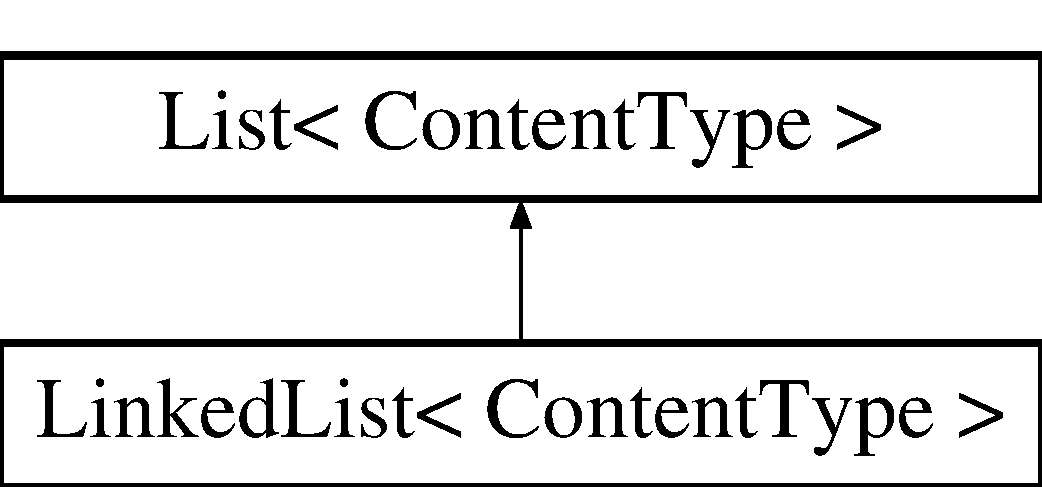
\includegraphics[height=2.000000cm]{class_list}
\end{center}
\end{figure}
\subsubsection*{Metody publiczne}
\begin{DoxyCompactItemize}
\item 
virtual int \& \hyperlink{class_list_a61bc4a0a8a2103d503f88b79d758f271}{size} ()=0
\begin{DoxyCompactList}\small\item\em Pobiera rozmiar listy. \end{DoxyCompactList}\item 
virtual Content\-Type \hyperlink{class_list_a3d0a41deda48ee401b45d4c74ad7f3fb}{pop\-\_\-back} ()=0
\begin{DoxyCompactList}\small\item\em Zwraca ostatni element z listy. \end{DoxyCompactList}\item 
virtual Content\-Type \hyperlink{class_list_abfc64c5f02d6aca4140e626c03ac8f7c}{pop\-\_\-front} ()=0
\begin{DoxyCompactList}\small\item\em Zwraca pierwszy element z listy. \end{DoxyCompactList}\item 
virtual void \hyperlink{class_list_ae9cd658323024b4fa3ce3be616d17f33}{print} ()=0
\begin{DoxyCompactList}\small\item\em Wyswietla liste. \end{DoxyCompactList}\item 
virtual void \hyperlink{class_list_aebfb58526e594d251d95d1a43bfa2edd}{push\-\_\-back} (Content\-Type \&arg)=0
\item 
virtual void \hyperlink{class_list_a2040f9141e0f48783aed547d7209904c}{push\-\_\-front} (Content\-Type \&arg)=0
\begin{DoxyCompactList}\small\item\em Wsadza Content\-Type do listy na poczatek. \end{DoxyCompactList}\item 
virtual Content\-Type \& \hyperlink{class_list_a85def545ed784186bc1cc8f47c80296e}{operator\mbox{[}$\,$\mbox{]}} (int number\-Of\-Element)=0
\begin{DoxyCompactList}\small\item\em Wsadza Content\-Type do listy na koniec. \end{DoxyCompactList}\item 
virtual void \hyperlink{class_list_ade0efb407e46f2f049e07159da017996}{insert\-After} (Content\-Type \&arg, int iterator\-I\-D)=0
\begin{DoxyCompactList}\small\item\em Wsadza Content\-Type po elemencie. \end{DoxyCompactList}\item 
virtual Content\-Type \& \hyperlink{class_list_a2c7a4d0c74230bbf7486026cc25952fb}{show\-\_\-front} ()=0
\begin{DoxyCompactList}\small\item\em Pokazue pierwszy element na liscie. \end{DoxyCompactList}\item 
virtual Content\-Type \& \hyperlink{class_list_ae6d8b6a4b0e8c18eca287821cbf3ee86}{show\-\_\-back} ()=0
\begin{DoxyCompactList}\small\item\em Pokazue ostatni element na liscie. \end{DoxyCompactList}\item 
virtual void \hyperlink{class_list_a8a1ebc7ce83d77b83f58bd8c2ce2d683}{clone\-From} (\hyperlink{class_list}{List}$<$ Content\-Type $>$ \&pattern\-List)
\begin{DoxyCompactList}\small\item\em Klonuje listy przydzielajac dla nowej nową pamięć dla każdego z jej elementu. \end{DoxyCompactList}\item 
virtual \hyperlink{class_list}{List}$<$ Content\-Type $>$ \& \hyperlink{class_list_a87870a63c8d7bb7530356d9278e766a9}{create\-Object\-From\-Abstract\-Reference} ()=0
\begin{DoxyCompactList}\small\item\em Wzorzec projektowy -\/ fabryki abstrakcyjnej. \end{DoxyCompactList}\item 
virtual void \hyperlink{class_list_a5c203187cbe44bdae313494542140a33}{free} ()
\begin{DoxyCompactList}\small\item\em Zwalnia zasoby listy. \end{DoxyCompactList}\item 
virtual \hyperlink{class_list_a93822e6461a4e3e084269edce851f7d3}{$\sim$\-List} ()
\end{DoxyCompactItemize}


\subsubsection{Opis szczegółowy}
\subsubsection*{template$<$class Content\-Type$>$class List$<$ Content\-Type $>$}

Interface dla klasy przedstawiających listy 

Definicja w linii \hyperlink{list_8h_source_l00016}{16} pliku \hyperlink{list_8h_source}{list.\-h}.



\subsubsection{Dokumentacja konstruktora i destruktora}
\hypertarget{class_list_a93822e6461a4e3e084269edce851f7d3}{\index{List@{List}!$\sim$\-List@{$\sim$\-List}}
\index{$\sim$\-List@{$\sim$\-List}!List@{List}}
\paragraph[{$\sim$\-List}]{\setlength{\rightskip}{0pt plus 5cm}template$<$class Content\-Type$>$ virtual {\bf List}$<$ Content\-Type $>$\-::$\sim${\bf List} (
\begin{DoxyParamCaption}
{}
\end{DoxyParamCaption}
)\hspace{0.3cm}{\ttfamily [inline]}, {\ttfamily [virtual]}}}\label{class_list_a93822e6461a4e3e084269edce851f7d3}


Definicja w linii \hyperlink{list_8h_source_l00083}{83} pliku \hyperlink{list_8h_source}{list.\-h}.


\begin{DoxyCode}
00083 \{\};
\end{DoxyCode}


\subsubsection{Dokumentacja funkcji składowych}
\hypertarget{class_list_a8a1ebc7ce83d77b83f58bd8c2ce2d683}{\index{List@{List}!clone\-From@{clone\-From}}
\index{clone\-From@{clone\-From}!List@{List}}
\paragraph[{clone\-From}]{\setlength{\rightskip}{0pt plus 5cm}template$<$class Content\-Type$>$ virtual void {\bf List}$<$ Content\-Type $>$\-::clone\-From (
\begin{DoxyParamCaption}
\item[{{\bf List}$<$ Content\-Type $>$ \&}]{pattern\-List}
\end{DoxyParamCaption}
)\hspace{0.3cm}{\ttfamily [inline]}, {\ttfamily [virtual]}}}\label{class_list_a8a1ebc7ce83d77b83f58bd8c2ce2d683}


Definicja w linii \hyperlink{list_8h_source_l00068}{68} pliku \hyperlink{list_8h_source}{list.\-h}.



Odwołania w \hyperlink{quicksorter_8h_source_l00028}{Quick\-Sorter$<$ Content\-Type $>$\-::\-Quick\-Sorter()}.


\begin{DoxyCode}
00069         \{
00070                 \textcolor{comment}{// release memory from main list}
00071                 \textcolor{keywordflow}{while}(this->\hyperlink{class_list_a61bc4a0a8a2103d503f88b79d758f271}{size}()) \hyperlink{class_list_a3d0a41deda48ee401b45d4c74ad7f3fb}{pop\_back}();
00072                 \textcolor{keywordflow}{for}(\textcolor{keywordtype}{int} i=0; i<patternList.\hyperlink{class_list_a61bc4a0a8a2103d503f88b79d758f271}{size}(); i++)
00073                         this->\hyperlink{class_list_aebfb58526e594d251d95d1a43bfa2edd}{push\_back}(patternList[i]);
00074         \}
\end{DoxyCode}
\hypertarget{class_list_a87870a63c8d7bb7530356d9278e766a9}{\index{List@{List}!create\-Object\-From\-Abstract\-Reference@{create\-Object\-From\-Abstract\-Reference}}
\index{create\-Object\-From\-Abstract\-Reference@{create\-Object\-From\-Abstract\-Reference}!List@{List}}
\paragraph[{create\-Object\-From\-Abstract\-Reference}]{\setlength{\rightskip}{0pt plus 5cm}template$<$class Content\-Type$>$ virtual {\bf List}$<$Content\-Type$>$\& {\bf List}$<$ Content\-Type $>$\-::create\-Object\-From\-Abstract\-Reference (
\begin{DoxyParamCaption}
{}
\end{DoxyParamCaption}
)\hspace{0.3cm}{\ttfamily [pure virtual]}}}\label{class_list_a87870a63c8d7bb7530356d9278e766a9}


Implementowany w \hyperlink{class_linked_list_aea53fafbbe620165ec3173ad3566785d}{Linked\-List$<$ Content\-Type $>$}, \hyperlink{class_linked_list_aea53fafbbe620165ec3173ad3566785d}{Linked\-List$<$ int $>$} i \hyperlink{class_linked_list_aea53fafbbe620165ec3173ad3566785d}{Linked\-List$<$ Observer $\ast$ $>$}.

\hypertarget{class_list_a5c203187cbe44bdae313494542140a33}{\index{List@{List}!free@{free}}
\index{free@{free}!List@{List}}
\paragraph[{free}]{\setlength{\rightskip}{0pt plus 5cm}template$<$class Content\-Type$>$ virtual void {\bf List}$<$ Content\-Type $>$\-::free (
\begin{DoxyParamCaption}
{}
\end{DoxyParamCaption}
)\hspace{0.3cm}{\ttfamily [inline]}, {\ttfamily [virtual]}}}\label{class_list_a5c203187cbe44bdae313494542140a33}


Definicja w linii \hyperlink{list_8h_source_l00082}{82} pliku \hyperlink{list_8h_source}{list.\-h}.


\begin{DoxyCode}
00082 \{ \textcolor{keywordflow}{while}(\hyperlink{class_list_a61bc4a0a8a2103d503f88b79d758f271}{size}()) \hyperlink{class_list_a3d0a41deda48ee401b45d4c74ad7f3fb}{pop\_back}(); \}
\end{DoxyCode}
\hypertarget{class_list_ade0efb407e46f2f049e07159da017996}{\index{List@{List}!insert\-After@{insert\-After}}
\index{insert\-After@{insert\-After}!List@{List}}
\paragraph[{insert\-After}]{\setlength{\rightskip}{0pt plus 5cm}template$<$class Content\-Type$>$ virtual void {\bf List}$<$ Content\-Type $>$\-::insert\-After (
\begin{DoxyParamCaption}
\item[{Content\-Type \&}]{arg, }
\item[{int}]{iterator\-I\-D}
\end{DoxyParamCaption}
)\hspace{0.3cm}{\ttfamily [pure virtual]}}}\label{class_list_ade0efb407e46f2f049e07159da017996}

\begin{DoxyParams}{Parametry}
{\em arg} & Element do wsadzenia \\
\hline
{\em iterator\-I\-D} & id elementu do wsadzenia \\
\hline
\end{DoxyParams}


Implementowany w \hyperlink{class_linked_list_aa882477023311c1400a724edd415e362}{Linked\-List$<$ Content\-Type $>$}, \hyperlink{class_linked_list_aa882477023311c1400a724edd415e362}{Linked\-List$<$ int $>$} i \hyperlink{class_linked_list_aa882477023311c1400a724edd415e362}{Linked\-List$<$ Observer $\ast$ $>$}.

\hypertarget{class_list_a85def545ed784186bc1cc8f47c80296e}{\index{List@{List}!operator\mbox{[}$\,$\mbox{]}@{operator[]}}
\index{operator\mbox{[}$\,$\mbox{]}@{operator[]}!List@{List}}
\paragraph[{operator[]}]{\setlength{\rightskip}{0pt plus 5cm}template$<$class Content\-Type$>$ virtual Content\-Type\& {\bf List}$<$ Content\-Type $>$\-::operator\mbox{[}$\,$\mbox{]} (
\begin{DoxyParamCaption}
\item[{int}]{number\-Of\-Element}
\end{DoxyParamCaption}
)\hspace{0.3cm}{\ttfamily [pure virtual]}}}\label{class_list_a85def545ed784186bc1cc8f47c80296e}


Implementowany w \hyperlink{class_linked_list_ad99e35cef5826d1cd456713ff8358a86}{Linked\-List$<$ Content\-Type $>$}, \hyperlink{class_linked_list_ad99e35cef5826d1cd456713ff8358a86}{Linked\-List$<$ int $>$} i \hyperlink{class_linked_list_ad99e35cef5826d1cd456713ff8358a86}{Linked\-List$<$ Observer $\ast$ $>$}.

\hypertarget{class_list_a3d0a41deda48ee401b45d4c74ad7f3fb}{\index{List@{List}!pop\-\_\-back@{pop\-\_\-back}}
\index{pop\-\_\-back@{pop\-\_\-back}!List@{List}}
\paragraph[{pop\-\_\-back}]{\setlength{\rightskip}{0pt plus 5cm}template$<$class Content\-Type$>$ virtual Content\-Type {\bf List}$<$ Content\-Type $>$\-::pop\-\_\-back (
\begin{DoxyParamCaption}
{}
\end{DoxyParamCaption}
)\hspace{0.3cm}{\ttfamily [pure virtual]}}}\label{class_list_a3d0a41deda48ee401b45d4c74ad7f3fb}
\begin{DoxyReturn}{Zwraca}
ostatni element z listy 
\end{DoxyReturn}


Implementowany w \hyperlink{class_linked_list_ad7634e21b0ccd370906c4f28baaffa38}{Linked\-List$<$ Content\-Type $>$}, \hyperlink{class_linked_list_ad7634e21b0ccd370906c4f28baaffa38}{Linked\-List$<$ int $>$} i \hyperlink{class_linked_list_ad7634e21b0ccd370906c4f28baaffa38}{Linked\-List$<$ Observer $\ast$ $>$}.



Odwołania w \hyperlink{list_8h_source_l00068}{List$<$ Observer $\ast$ $>$\-::clone\-From()} i \hyperlink{list_8h_source_l00082}{List$<$ Observer $\ast$ $>$\-::free()}.

\hypertarget{class_list_abfc64c5f02d6aca4140e626c03ac8f7c}{\index{List@{List}!pop\-\_\-front@{pop\-\_\-front}}
\index{pop\-\_\-front@{pop\-\_\-front}!List@{List}}
\paragraph[{pop\-\_\-front}]{\setlength{\rightskip}{0pt plus 5cm}template$<$class Content\-Type$>$ virtual Content\-Type {\bf List}$<$ Content\-Type $>$\-::pop\-\_\-front (
\begin{DoxyParamCaption}
{}
\end{DoxyParamCaption}
)\hspace{0.3cm}{\ttfamily [pure virtual]}}}\label{class_list_abfc64c5f02d6aca4140e626c03ac8f7c}
\begin{DoxyReturn}{Zwraca}
pierwszy element z listy 
\end{DoxyReturn}


Implementowany w \hyperlink{class_linked_list_a64abea886f0dadf69a3726d1880c514a}{Linked\-List$<$ Content\-Type $>$}, \hyperlink{class_linked_list_a64abea886f0dadf69a3726d1880c514a}{Linked\-List$<$ int $>$} i \hyperlink{class_linked_list_a64abea886f0dadf69a3726d1880c514a}{Linked\-List$<$ Observer $\ast$ $>$}.

\hypertarget{class_list_ae9cd658323024b4fa3ce3be616d17f33}{\index{List@{List}!print@{print}}
\index{print@{print}!List@{List}}
\paragraph[{print}]{\setlength{\rightskip}{0pt plus 5cm}template$<$class Content\-Type$>$ virtual void {\bf List}$<$ Content\-Type $>$\-::print (
\begin{DoxyParamCaption}
{}
\end{DoxyParamCaption}
)\hspace{0.3cm}{\ttfamily [pure virtual]}}}\label{class_list_ae9cd658323024b4fa3ce3be616d17f33}


Implementowany w \hyperlink{class_linked_list_a245ba50906c85c1765a5f611d3f3b6c0}{Linked\-List$<$ Content\-Type $>$}, \hyperlink{class_linked_list_a245ba50906c85c1765a5f611d3f3b6c0}{Linked\-List$<$ int $>$} i \hyperlink{class_linked_list_a245ba50906c85c1765a5f611d3f3b6c0}{Linked\-List$<$ Observer $\ast$ $>$}.

\hypertarget{class_list_aebfb58526e594d251d95d1a43bfa2edd}{\index{List@{List}!push\-\_\-back@{push\-\_\-back}}
\index{push\-\_\-back@{push\-\_\-back}!List@{List}}
\paragraph[{push\-\_\-back}]{\setlength{\rightskip}{0pt plus 5cm}template$<$class Content\-Type$>$ virtual void {\bf List}$<$ Content\-Type $>$\-::push\-\_\-back (
\begin{DoxyParamCaption}
\item[{Content\-Type \&}]{arg}
\end{DoxyParamCaption}
)\hspace{0.3cm}{\ttfamily [pure virtual]}}}\label{class_list_aebfb58526e594d251d95d1a43bfa2edd}


Implementowany w \hyperlink{class_linked_list_a719c7b47925171fd7a72a35d0a581619}{Linked\-List$<$ Content\-Type $>$}, \hyperlink{class_linked_list_a719c7b47925171fd7a72a35d0a581619}{Linked\-List$<$ int $>$} i \hyperlink{class_linked_list_a719c7b47925171fd7a72a35d0a581619}{Linked\-List$<$ Observer $\ast$ $>$}.



Odwołania w \hyperlink{list_8h_source_l00068}{List$<$ Observer $\ast$ $>$\-::clone\-From()}.

\hypertarget{class_list_a2040f9141e0f48783aed547d7209904c}{\index{List@{List}!push\-\_\-front@{push\-\_\-front}}
\index{push\-\_\-front@{push\-\_\-front}!List@{List}}
\paragraph[{push\-\_\-front}]{\setlength{\rightskip}{0pt plus 5cm}template$<$class Content\-Type$>$ virtual void {\bf List}$<$ Content\-Type $>$\-::push\-\_\-front (
\begin{DoxyParamCaption}
\item[{Content\-Type \&}]{arg}
\end{DoxyParamCaption}
)\hspace{0.3cm}{\ttfamily [pure virtual]}}}\label{class_list_a2040f9141e0f48783aed547d7209904c}


Implementowany w \hyperlink{class_linked_list_a9effa3698ad28e2f3401cd199f852e08}{Linked\-List$<$ Content\-Type $>$}, \hyperlink{class_linked_list_a9effa3698ad28e2f3401cd199f852e08}{Linked\-List$<$ int $>$} i \hyperlink{class_linked_list_a9effa3698ad28e2f3401cd199f852e08}{Linked\-List$<$ Observer $\ast$ $>$}.

\hypertarget{class_list_ae6d8b6a4b0e8c18eca287821cbf3ee86}{\index{List@{List}!show\-\_\-back@{show\-\_\-back}}
\index{show\-\_\-back@{show\-\_\-back}!List@{List}}
\paragraph[{show\-\_\-back}]{\setlength{\rightskip}{0pt plus 5cm}template$<$class Content\-Type$>$ virtual Content\-Type\& {\bf List}$<$ Content\-Type $>$\-::show\-\_\-back (
\begin{DoxyParamCaption}
{}
\end{DoxyParamCaption}
)\hspace{0.3cm}{\ttfamily [pure virtual]}}}\label{class_list_ae6d8b6a4b0e8c18eca287821cbf3ee86}


Implementowany w \hyperlink{class_linked_list_a437b5a0b96ab11f75e0391c76770186a}{Linked\-List$<$ Content\-Type $>$}, \hyperlink{class_linked_list_a437b5a0b96ab11f75e0391c76770186a}{Linked\-List$<$ int $>$} i \hyperlink{class_linked_list_a437b5a0b96ab11f75e0391c76770186a}{Linked\-List$<$ Observer $\ast$ $>$}.

\hypertarget{class_list_a2c7a4d0c74230bbf7486026cc25952fb}{\index{List@{List}!show\-\_\-front@{show\-\_\-front}}
\index{show\-\_\-front@{show\-\_\-front}!List@{List}}
\paragraph[{show\-\_\-front}]{\setlength{\rightskip}{0pt plus 5cm}template$<$class Content\-Type$>$ virtual Content\-Type\& {\bf List}$<$ Content\-Type $>$\-::show\-\_\-front (
\begin{DoxyParamCaption}
{}
\end{DoxyParamCaption}
)\hspace{0.3cm}{\ttfamily [pure virtual]}}}\label{class_list_a2c7a4d0c74230bbf7486026cc25952fb}


Implementowany w \hyperlink{class_linked_list_a2dcb9f488e5d179e89283a3f499acb76}{Linked\-List$<$ Content\-Type $>$}, \hyperlink{class_linked_list_a2dcb9f488e5d179e89283a3f499acb76}{Linked\-List$<$ int $>$} i \hyperlink{class_linked_list_a2dcb9f488e5d179e89283a3f499acb76}{Linked\-List$<$ Observer $\ast$ $>$}.

\hypertarget{class_list_a61bc4a0a8a2103d503f88b79d758f271}{\index{List@{List}!size@{size}}
\index{size@{size}!List@{List}}
\paragraph[{size}]{\setlength{\rightskip}{0pt plus 5cm}template$<$class Content\-Type$>$ virtual int\& {\bf List}$<$ Content\-Type $>$\-::size (
\begin{DoxyParamCaption}
{}
\end{DoxyParamCaption}
)\hspace{0.3cm}{\ttfamily [pure virtual]}}}\label{class_list_a61bc4a0a8a2103d503f88b79d758f271}
\begin{DoxyReturn}{Zwraca}
Rozmiar listy 
\end{DoxyReturn}


Implementowany w \hyperlink{class_linked_list_ab399f1dc929c705e9cba628ae1f29254}{Linked\-List$<$ Content\-Type $>$}, \hyperlink{class_linked_list_ab399f1dc929c705e9cba628ae1f29254}{Linked\-List$<$ int $>$} i \hyperlink{class_linked_list_ab399f1dc929c705e9cba628ae1f29254}{Linked\-List$<$ Observer $\ast$ $>$}.



Odwołania w \hyperlink{list_8h_source_l00068}{List$<$ Observer $\ast$ $>$\-::clone\-From()}, \hyperlink{list_8h_source_l00082}{List$<$ Observer $\ast$ $>$\-::free()} i \hyperlink{linkedlist_8h_source_l00047}{Linked\-List$<$ Observer $\ast$ $>$\-::\-Linked\-List()}.



Dokumentacja dla tej klasy została wygenerowana z pliku\-:\begin{DoxyCompactItemize}
\item 
\hyperlink{list_8h}{list.\-h}\end{DoxyCompactItemize}

\hypertarget{class_list_saver}{\subsection{Dokumentacja szablonu klasy List\-Saver$<$ Content\-Type $>$}
\label{class_list_saver}\index{List\-Saver$<$ Content\-Type $>$@{List\-Saver$<$ Content\-Type $>$}}
}


{\ttfamily \#include $<$listsaver.\-h$>$}

\subsubsection*{Metody prywatne}
\begin{DoxyCompactItemize}
\item 
\hyperlink{class_list_saver_ac4ad5223df78883a0301c3835a0eae55}{List\-Saver} (My\-List$<$ Content\-Type $>$ \&list\-Argument)
\begin{DoxyCompactList}\small\item\em Konstruktor pobierajacy referencje do listy do zapisu. \end{DoxyCompactList}\item 
void \hyperlink{class_list_saver_afd2e2fed3c727a4f025e3ec3ab3d3831}{save\-To\-File} (std\-::string nazwa\-Pliku)
\begin{DoxyCompactList}\small\item\em Zapisuje liste do pliku. \end{DoxyCompactList}\end{DoxyCompactItemize}
\subsubsection*{Atrybuty prywatne}
\begin{DoxyCompactItemize}
\item 
\hyperlink{class_list}{List}$<$ Content\-Type $>$ \& \hyperlink{class_list_saver_a6af039caf1e8895cf77097a942bd870d}{list}
\begin{DoxyCompactList}\small\item\em Klasa pozwalająca na zapis Listy do pliku. \end{DoxyCompactList}\end{DoxyCompactItemize}


\subsubsection{Opis szczegółowy}
\subsubsection*{template$<$class Content\-Type$>$class List\-Saver$<$ Content\-Type $>$}



Definicja w linii \hyperlink{listsaver_8h_source_l00015}{15} pliku \hyperlink{listsaver_8h_source}{listsaver.\-h}.



\subsubsection{Dokumentacja konstruktora i destruktora}
\hypertarget{class_list_saver_ac4ad5223df78883a0301c3835a0eae55}{\index{List\-Saver@{List\-Saver}!List\-Saver@{List\-Saver}}
\index{List\-Saver@{List\-Saver}!ListSaver@{List\-Saver}}
\paragraph[{List\-Saver}]{\setlength{\rightskip}{0pt plus 5cm}template$<$class Content\-Type $>$ {\bf List\-Saver}$<$ Content\-Type $>$\-::{\bf List\-Saver} (
\begin{DoxyParamCaption}
\item[{My\-List$<$ Content\-Type $>$ \&}]{list\-Argument}
\end{DoxyParamCaption}
)\hspace{0.3cm}{\ttfamily [inline]}, {\ttfamily [private]}}}\label{class_list_saver_ac4ad5223df78883a0301c3835a0eae55}

\begin{DoxyParams}{Parametry}
{\em list\-Argument} & lista do zapisu \\
\hline
\end{DoxyParams}


Definicja w linii \hyperlink{listsaver_8h_source_l00024}{24} pliku \hyperlink{listsaver_8h_source}{listsaver.\-h}.


\begin{DoxyCode}
00024                                                     :
00025                 \hyperlink{class_list_saver_a6af039caf1e8895cf77097a942bd870d}{list}(listArgument)
00026         \{\}
\end{DoxyCode}


\subsubsection{Dokumentacja funkcji składowych}
\hypertarget{class_list_saver_afd2e2fed3c727a4f025e3ec3ab3d3831}{\index{List\-Saver@{List\-Saver}!save\-To\-File@{save\-To\-File}}
\index{save\-To\-File@{save\-To\-File}!ListSaver@{List\-Saver}}
\paragraph[{save\-To\-File}]{\setlength{\rightskip}{0pt plus 5cm}template$<$class Content\-Type $>$ void {\bf List\-Saver}$<$ Content\-Type $>$\-::save\-To\-File (
\begin{DoxyParamCaption}
\item[{std\-::string}]{nazwa\-Pliku}
\end{DoxyParamCaption}
)\hspace{0.3cm}{\ttfamily [inline]}, {\ttfamily [private]}}}\label{class_list_saver_afd2e2fed3c727a4f025e3ec3ab3d3831}
\begin{DoxyReturn}{Zwraca}
Zwraca 0 gdy zapisywanie powiodlo sie 
\end{DoxyReturn}


Definicja w linii \hyperlink{listsaver_8h_source_l00032}{32} pliku \hyperlink{listsaver_8h_source}{listsaver.\-h}.



Odwołuje się do \hyperlink{listsaver_8h_source_l00019}{List\-Saver$<$ Content\-Type $>$\-::list}.


\begin{DoxyCode}
00033         \{
00034                 std::ofstream streamToFile;
00035                 streamToFile.open (nazwaPliku.c\_str(), std::ofstream::out);
00036                 \textcolor{keywordflow}{for}(\textcolor{keywordtype}{int} i=0; i<\hyperlink{class_list_saver_a6af039caf1e8895cf77097a942bd870d}{list}.size() ; i++)
00037                         streamToFile << \textcolor{charliteral}{'\{'}<<\hyperlink{class_list_saver_a6af039caf1e8895cf77097a942bd870d}{list}[i].content<<\textcolor{stringliteral}{"\} "};
00038                 streamToFile.close();
00039         \}
\end{DoxyCode}


\subsubsection{Dokumentacja atrybutów składowych}
\hypertarget{class_list_saver_a6af039caf1e8895cf77097a942bd870d}{\index{List\-Saver@{List\-Saver}!list@{list}}
\index{list@{list}!ListSaver@{List\-Saver}}
\paragraph[{list}]{\setlength{\rightskip}{0pt plus 5cm}template$<$class Content\-Type $>$ {\bf List}$<$Content\-Type$>$\& {\bf List\-Saver}$<$ Content\-Type $>$\-::list\hspace{0.3cm}{\ttfamily [private]}}}\label{class_list_saver_a6af039caf1e8895cf77097a942bd870d}


Definicja w linii \hyperlink{listsaver_8h_source_l00019}{19} pliku \hyperlink{listsaver_8h_source}{listsaver.\-h}.



Odwołania w \hyperlink{listsaver_8h_source_l00032}{List\-Saver$<$ Content\-Type $>$\-::save\-To\-File()}.



Dokumentacja dla tej klasy została wygenerowana z pliku\-:\begin{DoxyCompactItemize}
\item 
\hyperlink{listsaver_8h}{listsaver.\-h}\end{DoxyCompactItemize}

\hypertarget{class_merge_sorter}{\subsection{Dokumentacja szablonu klasy Merge\-Sorter$<$ My\-List\-Element\-Type $>$}
\label{class_merge_sorter}\index{Merge\-Sorter$<$ My\-List\-Element\-Type $>$@{Merge\-Sorter$<$ My\-List\-Element\-Type $>$}}
}


{\ttfamily \#include $<$mergesorter.\-h$>$}

Diagram dziedziczenia dla Merge\-Sorter$<$ My\-List\-Element\-Type $>$\begin{figure}[H]
\begin{center}
\leavevmode
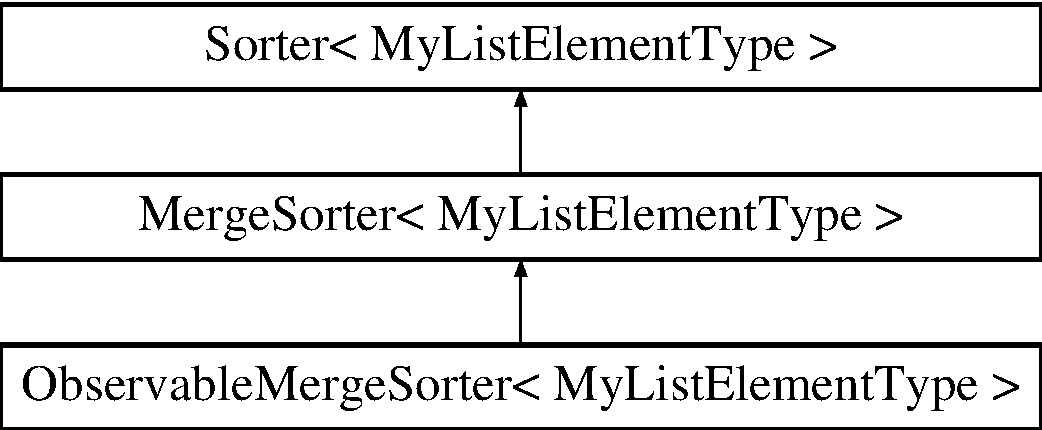
\includegraphics[height=3.000000cm]{class_merge_sorter}
\end{center}
\end{figure}
\subsubsection*{Metody publiczne}
\begin{DoxyCompactItemize}
\item 
\hyperlink{class_merge_sorter_a0ffb06429d7ebcb8bd007ca5db53429f}{Merge\-Sorter} (\hyperlink{class_my_list}{My\-List}$<$ My\-List\-Element\-Type $>$ \&list\-Arg)
\item 
virtual \hyperlink{class_merge_sorter_aa3e8fe75440511195aaf6dd7ef9dfcf1}{$\sim$\-Merge\-Sorter} ()
\item 
\hyperlink{class_my_list}{My\-List}$<$ My\-List\-Element\-Type $>$ \hyperlink{class_merge_sorter_a9cde12ce9803e379ab421bf377103ba0}{merge} (\hyperlink{class_my_list}{My\-List}$<$ My\-List\-Element\-Type $>$ left, \hyperlink{class_my_list}{My\-List}$<$ My\-List\-Element\-Type $>$ right)
\item 
\hyperlink{class_my_list}{My\-List}$<$ My\-List\-Element\-Type $>$ \hyperlink{class_merge_sorter_ab945fd9934a6f47a851b40b23d18ee71}{merge\-Sort} (\hyperlink{class_my_list}{My\-List}$<$ My\-List\-Element\-Type $>$ m)
\begin{DoxyCompactList}\small\item\em Sortuje liste przez scalanie. \end{DoxyCompactList}\item 
\hyperlink{class_list}{List}$<$ My\-List\-Element\-Type $>$ \& \hyperlink{class_merge_sorter_aaee4333eb37af6401eca60da3398e507}{sort} ()
\end{DoxyCompactItemize}
\subsubsection*{Atrybuty publiczne}
\begin{DoxyCompactItemize}
\item 
\hyperlink{class_my_list}{My\-List}$<$ My\-List\-Element\-Type $>$ \& \hyperlink{class_merge_sorter_a8ac3ee938414809d7da627cf918f1f87}{list}
\end{DoxyCompactItemize}


\subsubsection{Opis szczegółowy}
\subsubsection*{template$<$class My\-List\-Element\-Type$>$class Merge\-Sorter$<$ My\-List\-Element\-Type $>$}



Definicja w linii \hyperlink{mergesorter_8h_source_l00015}{15} pliku \hyperlink{mergesorter_8h_source}{mergesorter.\-h}.



\subsubsection{Dokumentacja konstruktora i destruktora}
\hypertarget{class_merge_sorter_a0ffb06429d7ebcb8bd007ca5db53429f}{\index{Merge\-Sorter@{Merge\-Sorter}!Merge\-Sorter@{Merge\-Sorter}}
\index{Merge\-Sorter@{Merge\-Sorter}!MergeSorter@{Merge\-Sorter}}
\paragraph[{Merge\-Sorter}]{\setlength{\rightskip}{0pt plus 5cm}template$<$class My\-List\-Element\-Type $>$ {\bf Merge\-Sorter}$<$ My\-List\-Element\-Type $>$\-::{\bf Merge\-Sorter} (
\begin{DoxyParamCaption}
\item[{{\bf My\-List}$<$ My\-List\-Element\-Type $>$ \&}]{list\-Arg}
\end{DoxyParamCaption}
)\hspace{0.3cm}{\ttfamily [inline]}}}\label{class_merge_sorter_a0ffb06429d7ebcb8bd007ca5db53429f}


Definicja w linii \hyperlink{mergesorter_8h_source_l00020}{20} pliku \hyperlink{mergesorter_8h_source}{mergesorter.\-h}.


\begin{DoxyCode}
00021         :\hyperlink{class_merge_sorter_a8ac3ee938414809d7da627cf918f1f87}{list}(listArg)      \{\}
\end{DoxyCode}
\hypertarget{class_merge_sorter_aa3e8fe75440511195aaf6dd7ef9dfcf1}{\index{Merge\-Sorter@{Merge\-Sorter}!$\sim$\-Merge\-Sorter@{$\sim$\-Merge\-Sorter}}
\index{$\sim$\-Merge\-Sorter@{$\sim$\-Merge\-Sorter}!MergeSorter@{Merge\-Sorter}}
\paragraph[{$\sim$\-Merge\-Sorter}]{\setlength{\rightskip}{0pt plus 5cm}template$<$class My\-List\-Element\-Type $>$ virtual {\bf Merge\-Sorter}$<$ My\-List\-Element\-Type $>$\-::$\sim${\bf Merge\-Sorter} (
\begin{DoxyParamCaption}
{}
\end{DoxyParamCaption}
)\hspace{0.3cm}{\ttfamily [inline]}, {\ttfamily [virtual]}}}\label{class_merge_sorter_aa3e8fe75440511195aaf6dd7ef9dfcf1}


Definicja w linii \hyperlink{mergesorter_8h_source_l00023}{23} pliku \hyperlink{mergesorter_8h_source}{mergesorter.\-h}.


\begin{DoxyCode}
00023 \{\}
\end{DoxyCode}


\subsubsection{Dokumentacja funkcji składowych}
\hypertarget{class_merge_sorter_a9cde12ce9803e379ab421bf377103ba0}{\index{Merge\-Sorter@{Merge\-Sorter}!merge@{merge}}
\index{merge@{merge}!MergeSorter@{Merge\-Sorter}}
\paragraph[{merge}]{\setlength{\rightskip}{0pt plus 5cm}template$<$class My\-List\-Element\-Type $>$ {\bf My\-List}$<$My\-List\-Element\-Type$>$ {\bf Merge\-Sorter}$<$ My\-List\-Element\-Type $>$\-::merge (
\begin{DoxyParamCaption}
\item[{{\bf My\-List}$<$ My\-List\-Element\-Type $>$}]{left, }
\item[{{\bf My\-List}$<$ My\-List\-Element\-Type $>$}]{right}
\end{DoxyParamCaption}
)\hspace{0.3cm}{\ttfamily [inline]}}}\label{class_merge_sorter_a9cde12ce9803e379ab421bf377103ba0}


Definicja w linii \hyperlink{mergesorter_8h_source_l00026}{26} pliku \hyperlink{mergesorter_8h_source}{mergesorter.\-h}.



Odwołuje się do \hyperlink{mylist_8h_source_l00098}{My\-List$<$ My\-List\-Element\-Type $>$\-::pop\-\_\-front()}, \hyperlink{mylist_8h_source_l00112}{My\-List$<$ My\-List\-Element\-Type $>$\-::push\-\_\-back()}, \hyperlink{mylist_8h_source_l00139}{My\-List$<$ My\-List\-Element\-Type $>$\-::show\-\_\-front()} i \hyperlink{mylist_8h_source_l00066}{My\-List$<$ My\-List\-Element\-Type $>$\-::size()}.



Odwołania w \hyperlink{mergesorter_8h_source_l00063}{Merge\-Sorter$<$ My\-List\-Element\-Type $>$\-::merge\-Sort()}.


\begin{DoxyCode}
00027         \{
00028                 \hyperlink{class_my_list}{MyList<MyListElementType>} result;
00029                 \textcolor{comment}{//Gdy jest jeszcze cos do sortowania}
00030                 \textcolor{keywordflow}{while} (left.\hyperlink{class_my_list_a267f669859ef3541333082cad6b28ab7}{size}() > 0 || right.\hyperlink{class_my_list_a267f669859ef3541333082cad6b28ab7}{size}() > 0)
00031                 \{
00032                         \textcolor{comment}{// Jak oba to zamieniamy}
00033                         \textcolor{keywordflow}{if} (left.\hyperlink{class_my_list_a267f669859ef3541333082cad6b28ab7}{size}() > 0 && right.\hyperlink{class_my_list_a267f669859ef3541333082cad6b28ab7}{size}() > 0)
00034                         \{
00035                                 \textcolor{comment}{// Sprawdzam czy zamieniac}
00036                                 \textcolor{keywordflow}{if} (left.\hyperlink{class_my_list_a2fe6cb1e5caf9f1d7d9df4b44faf8506}{show\_front}() <= right.
      \hyperlink{class_my_list_a2fe6cb1e5caf9f1d7d9df4b44faf8506}{show\_front}())
00037                                         \{
00038                                                 result.\hyperlink{class_my_list_a52dad29ecf7522b86df8daa3aa74702d}{push\_back}(left.
      \hyperlink{class_my_list_a2fe6cb1e5caf9f1d7d9df4b44faf8506}{show\_front}()); left.\hyperlink{class_my_list_a675af07472a5b7dde7ca602abb420efa}{pop\_front}();
00039                                         \}
00040                                 \textcolor{keywordflow}{else}
00041                                 \{
00042                                         result.\hyperlink{class_my_list_a52dad29ecf7522b86df8daa3aa74702d}{push\_back}(right.
      \hyperlink{class_my_list_a2fe6cb1e5caf9f1d7d9df4b44faf8506}{show\_front}()); right.\hyperlink{class_my_list_a675af07472a5b7dde7ca602abb420efa}{pop\_front}();
00043                                 \}
00044                         \}
00045                         \textcolor{comment}{// pojedyncze listy (nieparzyse)}
00046                         \textcolor{keywordflow}{else} \textcolor{keywordflow}{if} (left.\hyperlink{class_my_list_a267f669859ef3541333082cad6b28ab7}{size}() > 0)
00047                         \{
00048                                 \textcolor{keywordflow}{for} (\textcolor{keywordtype}{int} i = 0; i < left.\hyperlink{class_my_list_a267f669859ef3541333082cad6b28ab7}{size}(); i++) result.
      \hyperlink{class_my_list_a52dad29ecf7522b86df8daa3aa74702d}{push\_back}(left[i].content); \textcolor{keywordflow}{break};
00049                         \}
00050                         \textcolor{comment}{// pojedyncze listy (nieparzyse- taka sama sytuacja jak wyzej)}
00051                         \textcolor{keywordflow}{else} \textcolor{keywordflow}{if} ((\textcolor{keywordtype}{int})right.\hyperlink{class_my_list_a267f669859ef3541333082cad6b28ab7}{size}() > 0)
00052                         \{
00053                                 \textcolor{keywordflow}{for} (\textcolor{keywordtype}{int} i = 0; i < (int)right.\hyperlink{class_my_list_a267f669859ef3541333082cad6b28ab7}{size}(); i++) result.
      \hyperlink{class_my_list_a52dad29ecf7522b86df8daa3aa74702d}{push\_back}(right[i].content); \textcolor{keywordflow}{break};
00054                         \}
00055                 \}
00056                 \textcolor{keywordflow}{return} result;
00057         \}
\end{DoxyCode}
\hypertarget{class_merge_sorter_ab945fd9934a6f47a851b40b23d18ee71}{\index{Merge\-Sorter@{Merge\-Sorter}!merge\-Sort@{merge\-Sort}}
\index{merge\-Sort@{merge\-Sort}!MergeSorter@{Merge\-Sorter}}
\paragraph[{merge\-Sort}]{\setlength{\rightskip}{0pt plus 5cm}template$<$class My\-List\-Element\-Type $>$ {\bf My\-List}$<$My\-List\-Element\-Type$>$ {\bf Merge\-Sorter}$<$ My\-List\-Element\-Type $>$\-::merge\-Sort (
\begin{DoxyParamCaption}
\item[{{\bf My\-List}$<$ My\-List\-Element\-Type $>$}]{m}
\end{DoxyParamCaption}
)\hspace{0.3cm}{\ttfamily [inline]}}}\label{class_merge_sorter_ab945fd9934a6f47a851b40b23d18ee71}

\begin{DoxyParams}{Parametry}
{\em m} & Lista do posotrowania \\
\hline
\end{DoxyParams}
\begin{DoxyReturn}{Zwraca}
zwraca posotrowana liste 
\end{DoxyReturn}


Definicja w linii \hyperlink{mergesorter_8h_source_l00063}{63} pliku \hyperlink{mergesorter_8h_source}{mergesorter.\-h}.



Odwołuje się do \hyperlink{mergesorter_8h_source_l00026}{Merge\-Sorter$<$ My\-List\-Element\-Type $>$\-::merge()}, \hyperlink{mylist_8h_source_l00112}{My\-List$<$ My\-List\-Element\-Type $>$\-::push\-\_\-back()} i \hyperlink{mylist_8h_source_l00066}{My\-List$<$ My\-List\-Element\-Type $>$\-::size()}.



Odwołania w \hyperlink{mergesorter_8h_source_l00083}{Merge\-Sorter$<$ My\-List\-Element\-Type $>$\-::sort()}.


\begin{DoxyCode}
00064         \{
00065                 \textcolor{keywordflow}{if} (m.\hyperlink{class_my_list_a267f669859ef3541333082cad6b28ab7}{size}() <= 1) \textcolor{keywordflow}{return} m; \textcolor{comment}{// gdy juz nic nie ma do sotrowania}
00066                 \hyperlink{class_my_list}{MyList<MyListElementType>} left, right, result;
00067                 \textcolor{keywordtype}{int} middle = (m.\hyperlink{class_my_list_a267f669859ef3541333082cad6b28ab7}{size}()+ 1) / 2; \textcolor{comment}{// anty-nieparzyscie}
00068                 \textcolor{keywordflow}{for} (\textcolor{keywordtype}{int} i = 0; i < middle; i++)
00069                         \{
00070                                 left.\hyperlink{class_my_list_a52dad29ecf7522b86df8daa3aa74702d}{push\_back}(m[i].content);
00071                         \}
00072                 \textcolor{keywordflow}{for} (\textcolor{keywordtype}{int} i = middle; i < m.\hyperlink{class_my_list_a267f669859ef3541333082cad6b28ab7}{size}(); i++)
00073                         \{
00074                                 right.\hyperlink{class_my_list_a52dad29ecf7522b86df8daa3aa74702d}{push\_back}(m[i].content);
00075                         \}
00076                 left = \hyperlink{class_merge_sorter_ab945fd9934a6f47a851b40b23d18ee71}{mergeSort}(left);
00077                 right = \hyperlink{class_merge_sorter_ab945fd9934a6f47a851b40b23d18ee71}{mergeSort}(right);
00078                 result = \hyperlink{class_merge_sorter_a9cde12ce9803e379ab421bf377103ba0}{merge}(left, right);
00079                 \textcolor{keywordflow}{return} result;
00080         \}
\end{DoxyCode}
\hypertarget{class_merge_sorter_aaee4333eb37af6401eca60da3398e507}{\index{Merge\-Sorter@{Merge\-Sorter}!sort@{sort}}
\index{sort@{sort}!MergeSorter@{Merge\-Sorter}}
\paragraph[{sort}]{\setlength{\rightskip}{0pt plus 5cm}template$<$class My\-List\-Element\-Type $>$ {\bf List}$<$My\-List\-Element\-Type$>$\& {\bf Merge\-Sorter}$<$ My\-List\-Element\-Type $>$\-::sort (
\begin{DoxyParamCaption}
{}
\end{DoxyParamCaption}
)\hspace{0.3cm}{\ttfamily [inline]}, {\ttfamily [virtual]}}}\label{class_merge_sorter_aaee4333eb37af6401eca60da3398e507}


Implementuje \hyperlink{class_sorter_a4a82d8151d6172802d1e60cb30c7d7d3}{Sorter$<$ My\-List\-Element\-Type $>$}.



Reimplementowana w \hyperlink{class_observable_merge_sorter_ac845eed6758733f3935ffb5aa0b5f64a}{Observable\-Merge\-Sorter$<$ My\-List\-Element\-Type $>$}.



Definicja w linii \hyperlink{mergesorter_8h_source_l00083}{83} pliku \hyperlink{mergesorter_8h_source}{mergesorter.\-h}.



Odwołuje się do \hyperlink{mergesorter_8h_source_l00018}{Merge\-Sorter$<$ My\-List\-Element\-Type $>$\-::list} i \hyperlink{mergesorter_8h_source_l00063}{Merge\-Sorter$<$ My\-List\-Element\-Type $>$\-::merge\-Sort()}.



Odwołania w \hyperlink{observablemergesorter_8h_source_l00023}{Observable\-Merge\-Sorter$<$ My\-List\-Element\-Type $>$\-::sort()}.


\begin{DoxyCode}
00084         \{
00085                 this->\hyperlink{class_merge_sorter_a8ac3ee938414809d7da627cf918f1f87}{list}=\hyperlink{class_merge_sorter_ab945fd9934a6f47a851b40b23d18ee71}{mergeSort}(this->\hyperlink{class_merge_sorter_a8ac3ee938414809d7da627cf918f1f87}{list});
00086                 \textcolor{keywordflow}{return} this->\hyperlink{class_merge_sorter_a8ac3ee938414809d7da627cf918f1f87}{list};
00087         \}
\end{DoxyCode}


\subsubsection{Dokumentacja atrybutów składowych}
\hypertarget{class_merge_sorter_a8ac3ee938414809d7da627cf918f1f87}{\index{Merge\-Sorter@{Merge\-Sorter}!list@{list}}
\index{list@{list}!MergeSorter@{Merge\-Sorter}}
\paragraph[{list}]{\setlength{\rightskip}{0pt plus 5cm}template$<$class My\-List\-Element\-Type $>$ {\bf My\-List}$<$My\-List\-Element\-Type$>$\& {\bf Merge\-Sorter}$<$ My\-List\-Element\-Type $>$\-::list}}\label{class_merge_sorter_a8ac3ee938414809d7da627cf918f1f87}


Definicja w linii \hyperlink{mergesorter_8h_source_l00018}{18} pliku \hyperlink{mergesorter_8h_source}{mergesorter.\-h}.



Odwołania w \hyperlink{observablemergesorter_8h_source_l00023}{Observable\-Merge\-Sorter$<$ My\-List\-Element\-Type $>$\-::sort()} i \hyperlink{mergesorter_8h_source_l00083}{Merge\-Sorter$<$ My\-List\-Element\-Type $>$\-::sort()}.



Dokumentacja dla tej klasy została wygenerowana z pliku\-:\begin{DoxyCompactItemize}
\item 
\hyperlink{mergesorter_8h}{mergesorter.\-h}\end{DoxyCompactItemize}

\hypertarget{class_my_benchmark}{\subsection{Dokumentacja klasy My\-Benchmark}
\label{class_my_benchmark}\index{My\-Benchmark@{My\-Benchmark}}
}


Klasa bazowa/interface do testowania algorytmu.  




{\ttfamily \#include $<$mybenchmark.\-h$>$}

Diagram dziedziczenia dla My\-Benchmark\begin{figure}[H]
\begin{center}
\leavevmode
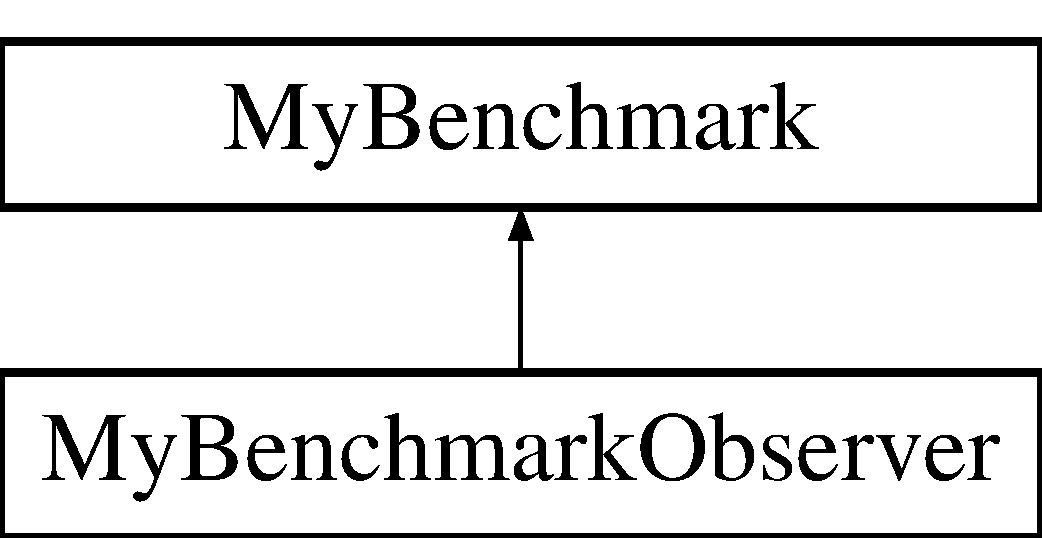
\includegraphics[height=2.000000cm]{class_my_benchmark}
\end{center}
\end{figure}
\subsubsection*{Metody publiczne}
\begin{DoxyCompactItemize}
\item 
\hyperlink{class_my_benchmark_a7f3739e8b61939627c0f63948a9975ca}{My\-Benchmark} ()
\item 
virtual \hyperlink{class_my_benchmark_a00de82c40680b41065eb402ac90f1736}{$\sim$\-My\-Benchmark} ()
\begin{DoxyCompactList}\small\item\em Usuwam obiekt test biorąc pod uwage jego prawdziwy typ. \end{DoxyCompactList}\end{DoxyCompactItemize}
\subsubsection*{Statyczne metody publiczne}
\begin{DoxyCompactItemize}
\item 
static void \hyperlink{class_my_benchmark_a802577db97fd440a3920add30c35a676}{timer\-Start} ()
\begin{DoxyCompactList}\small\item\em włączam stoper \end{DoxyCompactList}\item 
static double \hyperlink{class_my_benchmark_a7e3fa28fab999435bd4c51d915e42809}{timer\-Stop} ()
\begin{DoxyCompactList}\small\item\em wyłączam stoper \end{DoxyCompactList}\end{DoxyCompactItemize}
\subsubsection*{Atrybuty publiczne}
\begin{DoxyCompactItemize}
\item 
double \hyperlink{class_my_benchmark_a1cdab837ead670bd438f249ee82c8eff}{timer\-Value}
\begin{DoxyCompactList}\small\item\em Interface metody algorytmu glownego. \end{DoxyCompactList}\item 
std\-::ofstream \hyperlink{class_my_benchmark_a45b39f704800f8403789ff5c9bbb486b}{stream\-To\-File}
\end{DoxyCompactItemize}
\subsubsection*{Statyczne atrybuty publiczne}
\begin{DoxyCompactItemize}
\item 
static double \hyperlink{class_my_benchmark_aeca64d5b265e357ef879bf982dd4bb00}{timer\-Value\-Static} =0
\end{DoxyCompactItemize}


\subsubsection{Opis szczegółowy}
Używana jako interface dla wszystkich algorytmow aby testowac czas wykonywanego algorymtu. 

Definicja w linii \hyperlink{mybenchmark_8h_source_l00023}{23} pliku \hyperlink{mybenchmark_8h_source}{mybenchmark.\-h}.



\subsubsection{Dokumentacja konstruktora i destruktora}
\hypertarget{class_my_benchmark_a7f3739e8b61939627c0f63948a9975ca}{\index{My\-Benchmark@{My\-Benchmark}!My\-Benchmark@{My\-Benchmark}}
\index{My\-Benchmark@{My\-Benchmark}!MyBenchmark@{My\-Benchmark}}
\paragraph[{My\-Benchmark}]{\setlength{\rightskip}{0pt plus 5cm}My\-Benchmark\-::\-My\-Benchmark (
\begin{DoxyParamCaption}
{}
\end{DoxyParamCaption}
)\hspace{0.3cm}{\ttfamily [inline]}}}\label{class_my_benchmark_a7f3739e8b61939627c0f63948a9975ca}


Definicja w linii \hyperlink{mybenchmark_8h_source_l00043}{43} pliku \hyperlink{mybenchmark_8h_source}{mybenchmark.\-h}.



Odwołuje się do \hyperlink{mybenchmark_8h_source_l00041}{stream\-To\-File} i \hyperlink{mybenchmark_8h_source_l00040}{timer\-Value}.


\begin{DoxyCode}
00044         \{
00045                 \hyperlink{class_my_benchmark_a1cdab837ead670bd438f249ee82c8eff}{timerValue} = 0;
00046                 \hyperlink{class_my_benchmark_a45b39f704800f8403789ff5c9bbb486b}{streamToFile}.open (\textcolor{stringliteral}{"log.txt"}, std::ofstream::out  | std::ofstream::trunc);
00047                         \hyperlink{class_my_benchmark_a45b39f704800f8403789ff5c9bbb486b}{streamToFile}.close();
00048                 \hyperlink{class_my_benchmark_a45b39f704800f8403789ff5c9bbb486b}{streamToFile}.open (\textcolor{stringliteral}{"log.txt"}, std::ofstream::app);
00049                 \hyperlink{class_my_benchmark_a45b39f704800f8403789ff5c9bbb486b}{streamToFile} << std::fixed;
00050         \}
\end{DoxyCode}
\hypertarget{class_my_benchmark_a00de82c40680b41065eb402ac90f1736}{\index{My\-Benchmark@{My\-Benchmark}!$\sim$\-My\-Benchmark@{$\sim$\-My\-Benchmark}}
\index{$\sim$\-My\-Benchmark@{$\sim$\-My\-Benchmark}!MyBenchmark@{My\-Benchmark}}
\paragraph[{$\sim$\-My\-Benchmark}]{\setlength{\rightskip}{0pt plus 5cm}virtual My\-Benchmark\-::$\sim$\-My\-Benchmark (
\begin{DoxyParamCaption}
{}
\end{DoxyParamCaption}
)\hspace{0.3cm}{\ttfamily [inline]}, {\ttfamily [virtual]}}}\label{class_my_benchmark_a00de82c40680b41065eb402ac90f1736}


Definicja w linii \hyperlink{mybenchmark_8h_source_l00066}{66} pliku \hyperlink{mybenchmark_8h_source}{mybenchmark.\-h}.


\begin{DoxyCode}
00066 \{\};
\end{DoxyCode}


\subsubsection{Dokumentacja funkcji składowych}
\hypertarget{class_my_benchmark_a802577db97fd440a3920add30c35a676}{\index{My\-Benchmark@{My\-Benchmark}!timer\-Start@{timer\-Start}}
\index{timer\-Start@{timer\-Start}!MyBenchmark@{My\-Benchmark}}
\paragraph[{timer\-Start}]{\setlength{\rightskip}{0pt plus 5cm}void My\-Benchmark\-::timer\-Start (
\begin{DoxyParamCaption}
{}
\end{DoxyParamCaption}
)\hspace{0.3cm}{\ttfamily [static]}}}\label{class_my_benchmark_a802577db97fd440a3920add30c35a676}


Definicja w linii \hyperlink{mybenchmark_8cpp_source_l00012}{12} pliku \hyperlink{mybenchmark_8cpp_source}{mybenchmark.\-cpp}.



Odwołuje się do \hyperlink{mybenchmark_8h_source_l00042}{timer\-Value\-Static}.



Odwołania w \hyperlink{mybenchmark_8h_source_l00077}{My\-Benchmark\-Observer\-::received\-Start\-Update()}.


\begin{DoxyCode}
00013 \{
00014         \hyperlink{class_my_benchmark_aeca64d5b265e357ef879bf982dd4bb00}{MyBenchmark::timerValueStatic} = (( (double)clock() ) /CLOCKS\_PER\_SEC);
00015 \}
\end{DoxyCode}
\hypertarget{class_my_benchmark_a7e3fa28fab999435bd4c51d915e42809}{\index{My\-Benchmark@{My\-Benchmark}!timer\-Stop@{timer\-Stop}}
\index{timer\-Stop@{timer\-Stop}!MyBenchmark@{My\-Benchmark}}
\paragraph[{timer\-Stop}]{\setlength{\rightskip}{0pt plus 5cm}double My\-Benchmark\-::timer\-Stop (
\begin{DoxyParamCaption}
{}
\end{DoxyParamCaption}
)\hspace{0.3cm}{\ttfamily [static]}}}\label{class_my_benchmark_a7e3fa28fab999435bd4c51d915e42809}
\begin{DoxyReturn}{Zwraca}
Dlugosc dzialania stopera 
\end{DoxyReturn}


Definicja w linii \hyperlink{mybenchmark_8cpp_source_l00017}{17} pliku \hyperlink{mybenchmark_8cpp_source}{mybenchmark.\-cpp}.



Odwołuje się do \hyperlink{mybenchmark_8h_source_l00042}{timer\-Value\-Static}.



Odwołania w \hyperlink{mybenchmark_8h_source_l00082}{My\-Benchmark\-Observer\-::received\-Stop\-Update()} i \hyperlink{mybenchmark_8h_source_l00086}{My\-Benchmark\-Observer\-::received\-Stop\-Update\-And\-Save\-To\-File()}.


\begin{DoxyCode}
00018 \{
00019         \textcolor{keywordflow}{return} (( (\textcolor{keywordtype}{double})clock() ) /CLOCKS\_PER\_SEC) - 
      \hyperlink{class_my_benchmark_aeca64d5b265e357ef879bf982dd4bb00}{MyBenchmark::timerValueStatic};
00020 \}
\end{DoxyCode}


\subsubsection{Dokumentacja atrybutów składowych}
\hypertarget{class_my_benchmark_a45b39f704800f8403789ff5c9bbb486b}{\index{My\-Benchmark@{My\-Benchmark}!stream\-To\-File@{stream\-To\-File}}
\index{stream\-To\-File@{stream\-To\-File}!MyBenchmark@{My\-Benchmark}}
\paragraph[{stream\-To\-File}]{\setlength{\rightskip}{0pt plus 5cm}std\-::ofstream My\-Benchmark\-::stream\-To\-File}}\label{class_my_benchmark_a45b39f704800f8403789ff5c9bbb486b}


Definicja w linii \hyperlink{mybenchmark_8h_source_l00041}{41} pliku \hyperlink{mybenchmark_8h_source}{mybenchmark.\-h}.



Odwołania w \hyperlink{mybenchmark_8h_source_l00043}{My\-Benchmark()}, \hyperlink{mybenchmark_8h_source_l00086}{My\-Benchmark\-Observer\-::received\-Stop\-Update\-And\-Save\-To\-File()} i \hyperlink{mybenchmark_8h_source_l00092}{My\-Benchmark\-Observer\-::$\sim$\-My\-Benchmark\-Observer()}.

\hypertarget{class_my_benchmark_a1cdab837ead670bd438f249ee82c8eff}{\index{My\-Benchmark@{My\-Benchmark}!timer\-Value@{timer\-Value}}
\index{timer\-Value@{timer\-Value}!MyBenchmark@{My\-Benchmark}}
\paragraph[{timer\-Value}]{\setlength{\rightskip}{0pt plus 5cm}double My\-Benchmark\-::timer\-Value}}\label{class_my_benchmark_a1cdab837ead670bd438f249ee82c8eff}
Metoda abstrakcyjna, ktora jest interfacem do implementacji przez glowny algorytm. To znaczy, ze kazdy algorytm ma byc uruchamiany tą funkcja\-Czas stopera 

Definicja w linii \hyperlink{mybenchmark_8h_source_l00040}{40} pliku \hyperlink{mybenchmark_8h_source}{mybenchmark.\-h}.



Odwołania w \hyperlink{mybenchmark_8h_source_l00076}{My\-Benchmark\-Observer\-::get\-Timer\-Value()}, \hyperlink{mybenchmark_8h_source_l00043}{My\-Benchmark()} i \hyperlink{mybenchmark_8h_source_l00086}{My\-Benchmark\-Observer\-::received\-Stop\-Update\-And\-Save\-To\-File()}.

\hypertarget{class_my_benchmark_aeca64d5b265e357ef879bf982dd4bb00}{\index{My\-Benchmark@{My\-Benchmark}!timer\-Value\-Static@{timer\-Value\-Static}}
\index{timer\-Value\-Static@{timer\-Value\-Static}!MyBenchmark@{My\-Benchmark}}
\paragraph[{timer\-Value\-Static}]{\setlength{\rightskip}{0pt plus 5cm}double My\-Benchmark\-::timer\-Value\-Static =0\hspace{0.3cm}{\ttfamily [static]}}}\label{class_my_benchmark_aeca64d5b265e357ef879bf982dd4bb00}


Definicja w linii \hyperlink{mybenchmark_8h_source_l00042}{42} pliku \hyperlink{mybenchmark_8h_source}{mybenchmark.\-h}.



Odwołania w \hyperlink{mybenchmark_8cpp_source_l00012}{timer\-Start()} i \hyperlink{mybenchmark_8cpp_source_l00017}{timer\-Stop()}.



Dokumentacja dla tej klasy została wygenerowana z plików\-:\begin{DoxyCompactItemize}
\item 
\hyperlink{mybenchmark_8h}{mybenchmark.\-h}\item 
\hyperlink{mybenchmark_8cpp}{mybenchmark.\-cpp}\end{DoxyCompactItemize}

\hypertarget{class_my_benchmark_observer}{\subsection{Dokumentacja klasy My\-Benchmark\-Observer}
\label{class_my_benchmark_observer}\index{My\-Benchmark\-Observer@{My\-Benchmark\-Observer}}
}


{\ttfamily \#include $<$mybenchmark.\-h$>$}

Diagram dziedziczenia dla My\-Benchmark\-Observer\begin{figure}[H]
\begin{center}
\leavevmode
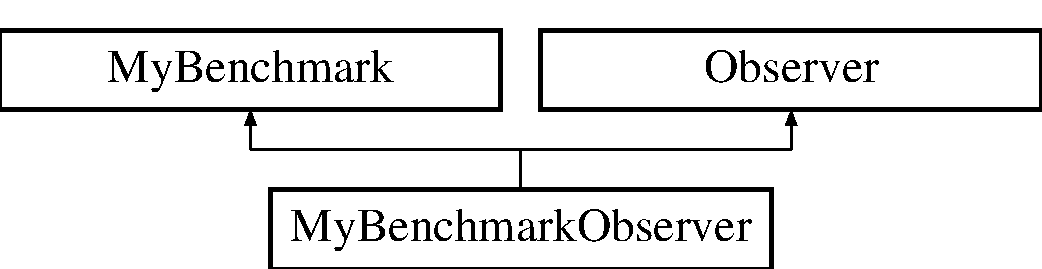
\includegraphics[height=2.000000cm]{class_my_benchmark_observer}
\end{center}
\end{figure}
\subsubsection*{Metody publiczne}
\begin{DoxyCompactItemize}
\item 
\hyperlink{class_my_benchmark_observer_ad65d0afb1ea49dbdebd1aef5f374aa9a}{My\-Benchmark\-Observer} ()
\item 
double \hyperlink{class_my_benchmark_observer_a33ea57a2d321f835f3af0d3bab76a931}{get\-Timer\-Value} ()
\item 
void \hyperlink{class_my_benchmark_observer_a50a758f459b683b82bbb32fa4c2f13df}{received\-Start\-Update} ()
\item 
void \hyperlink{class_my_benchmark_observer_aaf6a636ef6e8d8f8f8bc6d540e432246}{received\-Stop\-Update} ()
\item 
void \hyperlink{class_my_benchmark_observer_a2c12408a0f213a39d3419fd807f30968}{received\-Stop\-Update\-And\-Save\-To\-File} ()
\item 
virtual \hyperlink{class_my_benchmark_observer_addcc70a6c10af608874dc8613c84299f}{$\sim$\-My\-Benchmark\-Observer} ()
\end{DoxyCompactItemize}
\subsubsection*{Dodatkowe Dziedziczone Składowe}


\subsubsection{Opis szczegółowy}


Definicja w linii \hyperlink{mybenchmark_8h_source_l00072}{72} pliku \hyperlink{mybenchmark_8h_source}{mybenchmark.\-h}.



\subsubsection{Dokumentacja konstruktora i destruktora}
\hypertarget{class_my_benchmark_observer_ad65d0afb1ea49dbdebd1aef5f374aa9a}{\index{My\-Benchmark\-Observer@{My\-Benchmark\-Observer}!My\-Benchmark\-Observer@{My\-Benchmark\-Observer}}
\index{My\-Benchmark\-Observer@{My\-Benchmark\-Observer}!MyBenchmarkObserver@{My\-Benchmark\-Observer}}
\paragraph[{My\-Benchmark\-Observer}]{\setlength{\rightskip}{0pt plus 5cm}My\-Benchmark\-Observer\-::\-My\-Benchmark\-Observer (
\begin{DoxyParamCaption}
{}
\end{DoxyParamCaption}
)\hspace{0.3cm}{\ttfamily [inline]}}}\label{class_my_benchmark_observer_ad65d0afb1ea49dbdebd1aef5f374aa9a}


Definicja w linii \hyperlink{mybenchmark_8h_source_l00075}{75} pliku \hyperlink{mybenchmark_8h_source}{mybenchmark.\-h}.


\begin{DoxyCode}
00075 \{\};
\end{DoxyCode}
\hypertarget{class_my_benchmark_observer_addcc70a6c10af608874dc8613c84299f}{\index{My\-Benchmark\-Observer@{My\-Benchmark\-Observer}!$\sim$\-My\-Benchmark\-Observer@{$\sim$\-My\-Benchmark\-Observer}}
\index{$\sim$\-My\-Benchmark\-Observer@{$\sim$\-My\-Benchmark\-Observer}!MyBenchmarkObserver@{My\-Benchmark\-Observer}}
\paragraph[{$\sim$\-My\-Benchmark\-Observer}]{\setlength{\rightskip}{0pt plus 5cm}virtual My\-Benchmark\-Observer\-::$\sim$\-My\-Benchmark\-Observer (
\begin{DoxyParamCaption}
{}
\end{DoxyParamCaption}
)\hspace{0.3cm}{\ttfamily [inline]}, {\ttfamily [virtual]}}}\label{class_my_benchmark_observer_addcc70a6c10af608874dc8613c84299f}


Definicja w linii \hyperlink{mybenchmark_8h_source_l00092}{92} pliku \hyperlink{mybenchmark_8h_source}{mybenchmark.\-h}.



Odwołuje się do \hyperlink{mybenchmark_8h_source_l00041}{My\-Benchmark\-::stream\-To\-File}.


\begin{DoxyCode}
00092 \{\hyperlink{class_my_benchmark_a45b39f704800f8403789ff5c9bbb486b}{streamToFile}.close();\};
\end{DoxyCode}


\subsubsection{Dokumentacja funkcji składowych}
\hypertarget{class_my_benchmark_observer_a33ea57a2d321f835f3af0d3bab76a931}{\index{My\-Benchmark\-Observer@{My\-Benchmark\-Observer}!get\-Timer\-Value@{get\-Timer\-Value}}
\index{get\-Timer\-Value@{get\-Timer\-Value}!MyBenchmarkObserver@{My\-Benchmark\-Observer}}
\paragraph[{get\-Timer\-Value}]{\setlength{\rightskip}{0pt plus 5cm}double My\-Benchmark\-Observer\-::get\-Timer\-Value (
\begin{DoxyParamCaption}
{}
\end{DoxyParamCaption}
)\hspace{0.3cm}{\ttfamily [inline]}, {\ttfamily [virtual]}}}\label{class_my_benchmark_observer_a33ea57a2d321f835f3af0d3bab76a931}


Implementuje \hyperlink{class_observer_a5ea7b52632401a92b7ba0aca5bceceaa}{Observer}.



Definicja w linii \hyperlink{mybenchmark_8h_source_l00076}{76} pliku \hyperlink{mybenchmark_8h_source}{mybenchmark.\-h}.



Odwołuje się do \hyperlink{mybenchmark_8h_source_l00040}{My\-Benchmark\-::timer\-Value}.


\begin{DoxyCode}
00076 \{\textcolor{keywordflow}{return} this->\hyperlink{class_my_benchmark_a1cdab837ead670bd438f249ee82c8eff}{timerValue};\}
\end{DoxyCode}
\hypertarget{class_my_benchmark_observer_a50a758f459b683b82bbb32fa4c2f13df}{\index{My\-Benchmark\-Observer@{My\-Benchmark\-Observer}!received\-Start\-Update@{received\-Start\-Update}}
\index{received\-Start\-Update@{received\-Start\-Update}!MyBenchmarkObserver@{My\-Benchmark\-Observer}}
\paragraph[{received\-Start\-Update}]{\setlength{\rightskip}{0pt plus 5cm}void My\-Benchmark\-Observer\-::received\-Start\-Update (
\begin{DoxyParamCaption}
{}
\end{DoxyParamCaption}
)\hspace{0.3cm}{\ttfamily [inline]}, {\ttfamily [virtual]}}}\label{class_my_benchmark_observer_a50a758f459b683b82bbb32fa4c2f13df}


Implementuje \hyperlink{class_observer_a69ca89633f4624b79ec696a049793ba4}{Observer}.



Definicja w linii \hyperlink{mybenchmark_8h_source_l00077}{77} pliku \hyperlink{mybenchmark_8h_source}{mybenchmark.\-h}.



Odwołuje się do \hyperlink{mybenchmark_8cpp_source_l00012}{My\-Benchmark\-::timer\-Start()}.


\begin{DoxyCode}
00077                                     \{
00078                 \textcolor{comment}{//std::cout<<"\(\backslash\)nWlaczam stoper...";}
00079                 \hyperlink{class_my_benchmark_a802577db97fd440a3920add30c35a676}{timerStart}();
00080         \}
\end{DoxyCode}
\hypertarget{class_my_benchmark_observer_aaf6a636ef6e8d8f8f8bc6d540e432246}{\index{My\-Benchmark\-Observer@{My\-Benchmark\-Observer}!received\-Stop\-Update@{received\-Stop\-Update}}
\index{received\-Stop\-Update@{received\-Stop\-Update}!MyBenchmarkObserver@{My\-Benchmark\-Observer}}
\paragraph[{received\-Stop\-Update}]{\setlength{\rightskip}{0pt plus 5cm}void My\-Benchmark\-Observer\-::received\-Stop\-Update (
\begin{DoxyParamCaption}
{}
\end{DoxyParamCaption}
)\hspace{0.3cm}{\ttfamily [inline]}, {\ttfamily [virtual]}}}\label{class_my_benchmark_observer_aaf6a636ef6e8d8f8f8bc6d540e432246}


Implementuje \hyperlink{class_observer_a8eb646ac3407c4d24d01178a6ba74f7f}{Observer}.



Definicja w linii \hyperlink{mybenchmark_8h_source_l00082}{82} pliku \hyperlink{mybenchmark_8h_source}{mybenchmark.\-h}.



Odwołuje się do \hyperlink{mybenchmark_8cpp_source_l00017}{My\-Benchmark\-::timer\-Stop()}.


\begin{DoxyCode}
00082                                    \{
00083                 std::cout<<\textcolor{stringliteral}{"\(\backslash\)nCzas wykonywania operacji: "}<<\hyperlink{class_my_benchmark_a7e3fa28fab999435bd4c51d915e42809}{timerStop}();
00084         \}
\end{DoxyCode}
\hypertarget{class_my_benchmark_observer_a2c12408a0f213a39d3419fd807f30968}{\index{My\-Benchmark\-Observer@{My\-Benchmark\-Observer}!received\-Stop\-Update\-And\-Save\-To\-File@{received\-Stop\-Update\-And\-Save\-To\-File}}
\index{received\-Stop\-Update\-And\-Save\-To\-File@{received\-Stop\-Update\-And\-Save\-To\-File}!MyBenchmarkObserver@{My\-Benchmark\-Observer}}
\paragraph[{received\-Stop\-Update\-And\-Save\-To\-File}]{\setlength{\rightskip}{0pt plus 5cm}void My\-Benchmark\-Observer\-::received\-Stop\-Update\-And\-Save\-To\-File (
\begin{DoxyParamCaption}
{}
\end{DoxyParamCaption}
)\hspace{0.3cm}{\ttfamily [inline]}, {\ttfamily [virtual]}}}\label{class_my_benchmark_observer_a2c12408a0f213a39d3419fd807f30968}


Implementuje \hyperlink{class_observer_a764dd4568782b41271aa832edbe4455e}{Observer}.



Definicja w linii \hyperlink{mybenchmark_8h_source_l00086}{86} pliku \hyperlink{mybenchmark_8h_source}{mybenchmark.\-h}.



Odwołuje się do \hyperlink{mybenchmark_8h_source_l00041}{My\-Benchmark\-::stream\-To\-File}, \hyperlink{mybenchmark_8cpp_source_l00017}{My\-Benchmark\-::timer\-Stop()} i \hyperlink{mybenchmark_8h_source_l00040}{My\-Benchmark\-::timer\-Value}.


\begin{DoxyCode}
00086                                                 \{
00087                 \hyperlink{class_my_benchmark_a7e3fa28fab999435bd4c51d915e42809}{timerStop}();
00088                 \hyperlink{class_my_benchmark_a45b39f704800f8403789ff5c9bbb486b}{streamToFile}<<\hyperlink{class_my_benchmark_a1cdab837ead670bd438f249ee82c8eff}{timerValue}<<std::endl;
00089 
00090         \}
\end{DoxyCode}


Dokumentacja dla tej klasy została wygenerowana z pliku\-:\begin{DoxyCompactItemize}
\item 
\hyperlink{mybenchmark_8h}{mybenchmark.\-h}\end{DoxyCompactItemize}

\hypertarget{class_number_generator}{\subsection{Dokumentacja klasy Number\-Generator}
\label{class_number_generator}\index{Number\-Generator@{Number\-Generator}}
}


Klasa generujaca losowe liczby.  




{\ttfamily \#include $<$numbergenerator.\-h$>$}

\subsubsection*{Statyczne metody publiczne}
\begin{DoxyCompactItemize}
\item 
{\footnotesize template$<$typename Content\-Type $>$ }\\static \hyperlink{class_linked_list}{Linked\-List}$<$ Content\-Type $>$ \& \hyperlink{class_number_generator_a4a31ee39c34c77b01f19516fd5253389}{generate\-Numbers} (int range, int quantity)
\begin{DoxyCompactList}\small\item\em Generuje losowe liczby. \end{DoxyCompactList}\item 
static std\-::string $\ast$ \hyperlink{class_number_generator_afed5ae8efb72655770753790714b7643}{generate\-Strings} (int ile\-Stringow)
\begin{DoxyCompactList}\small\item\em Generuje losowe stringi. \end{DoxyCompactList}\end{DoxyCompactItemize}


\subsubsection{Opis szczegółowy}
Klasa generujaca losowe liczby na podstawie czasu maszyny na ktorym jest uruchomiona Wszystkie funkcje zapisu pliku dziedziczy z klasy Data\-Frame 

Definicja w linii \hyperlink{numbergenerator_8h_source_l00027}{27} pliku \hyperlink{numbergenerator_8h_source}{numbergenerator.\-h}.



\subsubsection{Dokumentacja funkcji składowych}
\hypertarget{class_number_generator_a4a31ee39c34c77b01f19516fd5253389}{\index{Number\-Generator@{Number\-Generator}!generate\-Numbers@{generate\-Numbers}}
\index{generate\-Numbers@{generate\-Numbers}!NumberGenerator@{Number\-Generator}}
\paragraph[{generate\-Numbers}]{\setlength{\rightskip}{0pt plus 5cm}template$<$typename Content\-Type $>$ static {\bf Linked\-List}$<$Content\-Type$>$\& Number\-Generator\-::generate\-Numbers (
\begin{DoxyParamCaption}
\item[{int}]{range, }
\item[{int}]{quantity}
\end{DoxyParamCaption}
)\hspace{0.3cm}{\ttfamily [inline]}, {\ttfamily [static]}}}\label{class_number_generator_a4a31ee39c34c77b01f19516fd5253389}


Definicja w linii \hyperlink{numbergenerator_8h_source_l00033}{33} pliku \hyperlink{numbergenerator_8h_source}{numbergenerator.\-h}.



Odwołuje się do \hyperlink{linkedlist_8h_source_l00100}{Linked\-List$<$ Content\-Type $>$\-::push\-\_\-back()}.


\begin{DoxyCode}
00034 \{
00035         \hyperlink{class_linked_list}{LinkedList<ContentType>} &myList = *\textcolor{keyword}{new} 
      \hyperlink{class_linked_list}{LinkedList<ContentType>}();
00036         time\_t randomTime = clock();
00037         \textcolor{keywordtype}{int} randomNumber;
00038         \textcolor{keywordflow}{for}(\textcolor{keywordtype}{int} i=0; i<quantity ; i++)
00039         \{
00040                 srand (randomTime = clock());
00041                 randomNumber = rand()%range;
00042                 myList.\hyperlink{class_linked_list_a719c7b47925171fd7a72a35d0a581619}{push\_back}(randomNumber);
00043                 randomTime = clock();
00044         \}
00045         \textcolor{keywordflow}{return} myList;
00046 \}
\end{DoxyCode}
\hypertarget{class_number_generator_afed5ae8efb72655770753790714b7643}{\index{Number\-Generator@{Number\-Generator}!generate\-Strings@{generate\-Strings}}
\index{generate\-Strings@{generate\-Strings}!NumberGenerator@{Number\-Generator}}
\paragraph[{generate\-Strings}]{\setlength{\rightskip}{0pt plus 5cm}static std\-::string$\ast$ Number\-Generator\-::generate\-Strings (
\begin{DoxyParamCaption}
\item[{int}]{ile\-Stringow}
\end{DoxyParamCaption}
)\hspace{0.3cm}{\ttfamily [static]}}}\label{class_number_generator_afed5ae8efb72655770753790714b7643}

\begin{DoxyParams}{Parametry}
{\em ile\-Stringow} & Ilosc stringow do stworzenia Generuje losowe stringi na podstawie czasu maszyny \\
\hline
\end{DoxyParams}


Dokumentacja dla tej klasy została wygenerowana z pliku\-:\begin{DoxyCompactItemize}
\item 
\hyperlink{numbergenerator_8h}{numbergenerator.\-h}\end{DoxyCompactItemize}

\hypertarget{class_observable}{\subsection{Dokumentacja klasy Observable}
\label{class_observable}\index{Observable@{Observable}}
}


Klasa abstrakcyjna-\/ bazowa dla objektow do obserowania.  




{\ttfamily \#include $<$observable.\-h$>$}

Diagram dziedziczenia dla Observable\begin{figure}[H]
\begin{center}
\leavevmode
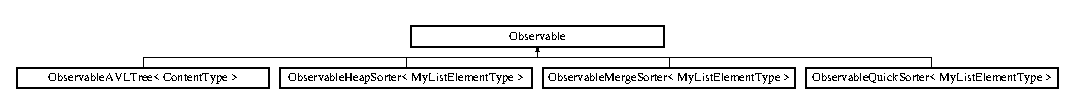
\includegraphics[height=1.282932cm]{class_observable}
\end{center}
\end{figure}
\subsubsection*{Metody publiczne}
\begin{DoxyCompactItemize}
\item 
void \hyperlink{class_observable_a18e7700c59126dbeb97d24844c6ed131}{add} (\hyperlink{class_observer}{Observer} $\ast$obserwator)
\begin{DoxyCompactList}\small\item\em Dodaje sie jako obiekt do obserowania dla danego obserwatora. \end{DoxyCompactList}\item 
void \hyperlink{class_observable_a78df64057f152342a43f27979186a6ba}{send\-Start\-Update\-To\-Observers} ()
\begin{DoxyCompactList}\small\item\em Wysyla powiadomienie do obserwatorow o rozpoczeciu algorytmu. \end{DoxyCompactList}\item 
void \hyperlink{class_observable_a16f75ed1514a0cb7526b5a5d2b7ca7c6}{send\-Stop\-Update\-To\-Observers} ()
\begin{DoxyCompactList}\small\item\em Wysyla powiadomienie do obserwatorow o zakonczeniu algorytmu. \end{DoxyCompactList}\item 
virtual \hyperlink{class_observable_a42f551d4d64ffa48a2ea8d7f0a4e42d4}{$\sim$\-Observable} ()
\end{DoxyCompactItemize}
\subsubsection*{Atrybuty publiczne}
\begin{DoxyCompactItemize}
\item 
\hyperlink{class_my_list}{My\-List}$<$ \hyperlink{class_observer}{Observer} $\ast$ $>$ \hyperlink{class_observable_a23f06cfbce27372d95fb556ca1f392ee}{observaters}
\begin{DoxyCompactList}\small\item\em Lista obserwatorow. \end{DoxyCompactList}\end{DoxyCompactItemize}


\subsubsection{Opis szczegółowy}


Definicja w linii \hyperlink{observable_8h_source_l00016}{16} pliku \hyperlink{observable_8h_source}{observable.\-h}.



\subsubsection{Dokumentacja konstruktora i destruktora}
\hypertarget{class_observable_a42f551d4d64ffa48a2ea8d7f0a4e42d4}{\index{Observable@{Observable}!$\sim$\-Observable@{$\sim$\-Observable}}
\index{$\sim$\-Observable@{$\sim$\-Observable}!Observable@{Observable}}
\paragraph[{$\sim$\-Observable}]{\setlength{\rightskip}{0pt plus 5cm}virtual Observable\-::$\sim$\-Observable (
\begin{DoxyParamCaption}
{}
\end{DoxyParamCaption}
)\hspace{0.3cm}{\ttfamily [inline]}, {\ttfamily [virtual]}}}\label{class_observable_a42f551d4d64ffa48a2ea8d7f0a4e42d4}


Definicja w linii \hyperlink{observable_8h_source_l00044}{44} pliku \hyperlink{observable_8h_source}{observable.\-h}.


\begin{DoxyCode}
00044 \{\}
\end{DoxyCode}


\subsubsection{Dokumentacja funkcji składowych}
\hypertarget{class_observable_a18e7700c59126dbeb97d24844c6ed131}{\index{Observable@{Observable}!add@{add}}
\index{add@{add}!Observable@{Observable}}
\paragraph[{add}]{\setlength{\rightskip}{0pt plus 5cm}void Observable\-::add (
\begin{DoxyParamCaption}
\item[{{\bf Observer} $\ast$}]{obserwator}
\end{DoxyParamCaption}
)\hspace{0.3cm}{\ttfamily [inline]}}}\label{class_observable_a18e7700c59126dbeb97d24844c6ed131}


Definicja w linii \hyperlink{observable_8h_source_l00023}{23} pliku \hyperlink{observable_8h_source}{observable.\-h}.



Odwołuje się do \hyperlink{observable_8h_source_l00019}{observaters} i \hyperlink{mylist_8h_source_l00112}{My\-List$<$ My\-List\-Element\-Type $>$\-::push\-\_\-back()}.



Odwołania w \hyperlink{main_8cpp_source_l00022}{main()}.


\begin{DoxyCode}
00023                                    \{
00024         \hyperlink{class_observable_a23f06cfbce27372d95fb556ca1f392ee}{observaters}.\hyperlink{class_my_list_a52dad29ecf7522b86df8daa3aa74702d}{push\_back}(obserwator);
00025     \}
\end{DoxyCode}
\hypertarget{class_observable_a78df64057f152342a43f27979186a6ba}{\index{Observable@{Observable}!send\-Start\-Update\-To\-Observers@{send\-Start\-Update\-To\-Observers}}
\index{send\-Start\-Update\-To\-Observers@{send\-Start\-Update\-To\-Observers}!Observable@{Observable}}
\paragraph[{send\-Start\-Update\-To\-Observers}]{\setlength{\rightskip}{0pt plus 5cm}void Observable\-::send\-Start\-Update\-To\-Observers (
\begin{DoxyParamCaption}
{}
\end{DoxyParamCaption}
)\hspace{0.3cm}{\ttfamily [inline]}}}\label{class_observable_a78df64057f152342a43f27979186a6ba}


Definicja w linii \hyperlink{observable_8h_source_l00029}{29} pliku \hyperlink{observable_8h_source}{observable.\-h}.



Odwołuje się do \hyperlink{observable_8h_source_l00019}{observaters} i \hyperlink{mylist_8h_source_l00066}{My\-List$<$ My\-List\-Element\-Type $>$\-::size()}.



Odwołania w \hyperlink{observableheapsorter_8h_source_l00026}{Observable\-Heap\-Sorter$<$ My\-List\-Element\-Type $>$\-::sort()}, \hyperlink{observablequicksorter_8h_source_l00026}{Observable\-Quick\-Sorter$<$ My\-List\-Element\-Type $>$\-::sort()} i \hyperlink{observablemergesorter_8h_source_l00026}{Observable\-Merge\-Sorter$<$ My\-List\-Element\-Type $>$\-::sort()}.


\begin{DoxyCode}
00029                                        \{
00030         \textcolor{keywordflow}{for}(\textcolor{keywordtype}{int} i=0; i<\hyperlink{class_observable_a23f06cfbce27372d95fb556ca1f392ee}{observaters}.\hyperlink{class_my_list_a267f669859ef3541333082cad6b28ab7}{size}(); i++)
00031         \{
00032                 \textcolor{comment}{//std::cout<<"Wysylam start update";}
00033                 \hyperlink{class_observable_a23f06cfbce27372d95fb556ca1f392ee}{observaters}[i].content->receivedStartUpdate();
00034         \}
00035     \}
\end{DoxyCode}
\hypertarget{class_observable_a16f75ed1514a0cb7526b5a5d2b7ca7c6}{\index{Observable@{Observable}!send\-Stop\-Update\-To\-Observers@{send\-Stop\-Update\-To\-Observers}}
\index{send\-Stop\-Update\-To\-Observers@{send\-Stop\-Update\-To\-Observers}!Observable@{Observable}}
\paragraph[{send\-Stop\-Update\-To\-Observers}]{\setlength{\rightskip}{0pt plus 5cm}void Observable\-::send\-Stop\-Update\-To\-Observers (
\begin{DoxyParamCaption}
{}
\end{DoxyParamCaption}
)\hspace{0.3cm}{\ttfamily [inline]}}}\label{class_observable_a16f75ed1514a0cb7526b5a5d2b7ca7c6}


Definicja w linii \hyperlink{observable_8h_source_l00039}{39} pliku \hyperlink{observable_8h_source}{observable.\-h}.



Odwołuje się do \hyperlink{observable_8h_source_l00019}{observaters} i \hyperlink{mylist_8h_source_l00066}{My\-List$<$ My\-List\-Element\-Type $>$\-::size()}.



Odwołania w \hyperlink{observableheapsorter_8h_source_l00026}{Observable\-Heap\-Sorter$<$ My\-List\-Element\-Type $>$\-::sort()}, \hyperlink{observablequicksorter_8h_source_l00026}{Observable\-Quick\-Sorter$<$ My\-List\-Element\-Type $>$\-::sort()} i \hyperlink{observablemergesorter_8h_source_l00026}{Observable\-Merge\-Sorter$<$ My\-List\-Element\-Type $>$\-::sort()}.


\begin{DoxyCode}
00039                                       \{
00040         \textcolor{keywordflow}{for}(\textcolor{keywordtype}{int} i=0; i<\hyperlink{class_observable_a23f06cfbce27372d95fb556ca1f392ee}{observaters}.\hyperlink{class_my_list_a267f669859ef3541333082cad6b28ab7}{size}(); i++)
00041                 \hyperlink{class_observable_a23f06cfbce27372d95fb556ca1f392ee}{observaters}[i].content->receivedStopUpdate();
00042     \}
\end{DoxyCode}


\subsubsection{Dokumentacja atrybutów składowych}
\hypertarget{class_observable_a23f06cfbce27372d95fb556ca1f392ee}{\index{Observable@{Observable}!observaters@{observaters}}
\index{observaters@{observaters}!Observable@{Observable}}
\paragraph[{observaters}]{\setlength{\rightskip}{0pt plus 5cm}{\bf My\-List}$<${\bf Observer}$\ast$$>$ Observable\-::observaters}}\label{class_observable_a23f06cfbce27372d95fb556ca1f392ee}


Definicja w linii \hyperlink{observable_8h_source_l00019}{19} pliku \hyperlink{observable_8h_source}{observable.\-h}.



Odwołania w \hyperlink{observable_8h_source_l00023}{add()}, \hyperlink{main_8cpp_source_l00022}{main()}, \hyperlink{observable_8h_source_l00029}{send\-Start\-Update\-To\-Observers()} i \hyperlink{observable_8h_source_l00039}{send\-Stop\-Update\-To\-Observers()}.



Dokumentacja dla tej klasy została wygenerowana z pliku\-:\begin{DoxyCompactItemize}
\item 
\hyperlink{observable_8h}{observable.\-h}\end{DoxyCompactItemize}

\hypertarget{class_observable_heap_sorter}{\subsection{Dokumentacja szablonu klasy Observable\-Heap\-Sorter$<$ Content\-Type $>$}
\label{class_observable_heap_sorter}\index{Observable\-Heap\-Sorter$<$ Content\-Type $>$@{Observable\-Heap\-Sorter$<$ Content\-Type $>$}}
}


Klasa sluzaca do obslugi sortowania przez kopcowanie z dodaniem obserwatora.  




{\ttfamily \#include $<$observableheapsorter.\-h$>$}

Diagram dziedziczenia dla Observable\-Heap\-Sorter$<$ Content\-Type $>$\begin{figure}[H]
\begin{center}
\leavevmode
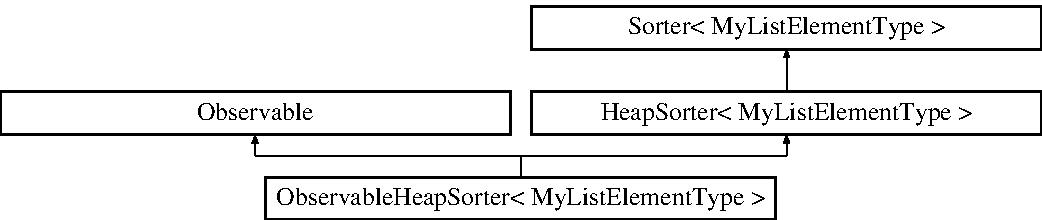
\includegraphics[height=3.000000cm]{class_observable_heap_sorter}
\end{center}
\end{figure}
\subsubsection*{Metody publiczne}
\begin{DoxyCompactItemize}
\item 
\hyperlink{class_observable_heap_sorter_afc6079c41bb8424c65d350d1287b5e0e}{Observable\-Heap\-Sorter} (\hyperlink{class_list}{List}$<$ Content\-Type $>$ \&my\-List)
\item 
\hyperlink{class_list}{List}$<$ Content\-Type $>$ \& \hyperlink{class_observable_heap_sorter_aa56ec2ca7bd6498f0a0085946c464f36}{sort} ()
\begin{DoxyCompactList}\small\item\em sortuje przez kopcowanie \end{DoxyCompactList}\item 
virtual \hyperlink{class_observable_heap_sorter_a048e01a7e09297b25dc2cb5b1996506b}{$\sim$\-Observable\-Heap\-Sorter} ()
\end{DoxyCompactItemize}
\subsubsection*{Dodatkowe Dziedziczone Składowe}


\subsubsection{Opis szczegółowy}
\subsubsection*{template$<$class Content\-Type$>$class Observable\-Heap\-Sorter$<$ Content\-Type $>$}



Definicja w linii \hyperlink{observableheapsorter_8h_source_l00018}{18} pliku \hyperlink{observableheapsorter_8h_source}{observableheapsorter.\-h}.



\subsubsection{Dokumentacja konstruktora i destruktora}
\hypertarget{class_observable_heap_sorter_afc6079c41bb8424c65d350d1287b5e0e}{\index{Observable\-Heap\-Sorter@{Observable\-Heap\-Sorter}!Observable\-Heap\-Sorter@{Observable\-Heap\-Sorter}}
\index{Observable\-Heap\-Sorter@{Observable\-Heap\-Sorter}!ObservableHeapSorter@{Observable\-Heap\-Sorter}}
\paragraph[{Observable\-Heap\-Sorter}]{\setlength{\rightskip}{0pt plus 5cm}template$<$class Content\-Type $>$ {\bf Observable\-Heap\-Sorter}$<$ Content\-Type $>$\-::{\bf Observable\-Heap\-Sorter} (
\begin{DoxyParamCaption}
\item[{{\bf List}$<$ Content\-Type $>$ \&}]{my\-List}
\end{DoxyParamCaption}
)\hspace{0.3cm}{\ttfamily [inline]}}}\label{class_observable_heap_sorter_afc6079c41bb8424c65d350d1287b5e0e}


Definicja w linii \hyperlink{observableheapsorter_8h_source_l00021}{21} pliku \hyperlink{observableheapsorter_8h_source}{observableheapsorter.\-h}.


\begin{DoxyCode}
00021                                                        :
00022                 \hyperlink{class_heap_sorter_a28b0447f09b338f37ab3413c2fb8a021}{HeapSorter<ContentType>::HeapSorter}(myList)\{\}
\end{DoxyCode}
\hypertarget{class_observable_heap_sorter_a048e01a7e09297b25dc2cb5b1996506b}{\index{Observable\-Heap\-Sorter@{Observable\-Heap\-Sorter}!$\sim$\-Observable\-Heap\-Sorter@{$\sim$\-Observable\-Heap\-Sorter}}
\index{$\sim$\-Observable\-Heap\-Sorter@{$\sim$\-Observable\-Heap\-Sorter}!ObservableHeapSorter@{Observable\-Heap\-Sorter}}
\paragraph[{$\sim$\-Observable\-Heap\-Sorter}]{\setlength{\rightskip}{0pt plus 5cm}template$<$class Content\-Type $>$ virtual {\bf Observable\-Heap\-Sorter}$<$ Content\-Type $>$\-::$\sim${\bf Observable\-Heap\-Sorter} (
\begin{DoxyParamCaption}
{}
\end{DoxyParamCaption}
)\hspace{0.3cm}{\ttfamily [inline]}, {\ttfamily [virtual]}}}\label{class_observable_heap_sorter_a048e01a7e09297b25dc2cb5b1996506b}


Definicja w linii \hyperlink{observableheapsorter_8h_source_l00033}{33} pliku \hyperlink{observableheapsorter_8h_source}{observableheapsorter.\-h}.


\begin{DoxyCode}
00033 \{\};
\end{DoxyCode}


\subsubsection{Dokumentacja funkcji składowych}
\hypertarget{class_observable_heap_sorter_aa56ec2ca7bd6498f0a0085946c464f36}{\index{Observable\-Heap\-Sorter@{Observable\-Heap\-Sorter}!sort@{sort}}
\index{sort@{sort}!ObservableHeapSorter@{Observable\-Heap\-Sorter}}
\paragraph[{sort}]{\setlength{\rightskip}{0pt plus 5cm}template$<$class Content\-Type $>$ {\bf List}$<$Content\-Type$>$\& {\bf Observable\-Heap\-Sorter}$<$ Content\-Type $>$\-::sort (
\begin{DoxyParamCaption}
{}
\end{DoxyParamCaption}
)\hspace{0.3cm}{\ttfamily [inline]}, {\ttfamily [virtual]}}}\label{class_observable_heap_sorter_aa56ec2ca7bd6498f0a0085946c464f36}


Reimplementowana z \hyperlink{class_heap_sorter_a0617d40d6d46a65535e7af76f2957898}{Heap\-Sorter$<$ Content\-Type $>$}.



Definicja w linii \hyperlink{observableheapsorter_8h_source_l00026}{26} pliku \hyperlink{observableheapsorter_8h_source}{observableheapsorter.\-h}.



Odwołuje się do \hyperlink{heapsorter_8h_source_l00021}{Heap\-Sorter$<$ Content\-Type $>$\-::list}, \hyperlink{observable_8h_source_l00029}{Observable\-::send\-Start\-Update\-To\-Observers()}, \hyperlink{observable_8h_source_l00039}{Observable\-::send\-Stop\-Update\-To\-Observers()} i \hyperlink{heapsorter_8h_source_l00042}{Heap\-Sorter$<$ Content\-Type $>$\-::sort()}.


\begin{DoxyCode}
00027         \{
00028                 \hyperlink{class_observable_a78df64057f152342a43f27979186a6ba}{sendStartUpdateToObservers}();
00029                 \hyperlink{class_heap_sorter_a0617d40d6d46a65535e7af76f2957898}{HeapSorter<ContentType>::sort}();
00030                 \hyperlink{class_observable_a16f75ed1514a0cb7526b5a5d2b7ca7c6}{sendStopUpdateToObservers}();
00031                 \textcolor{keywordflow}{return} this->\hyperlink{class_heap_sorter_ae5061b641a597893a2e7f747c9cc15f2}{list};
00032         \}
\end{DoxyCode}


Dokumentacja dla tej klasy została wygenerowana z pliku\-:\begin{DoxyCompactItemize}
\item 
\hyperlink{observableheapsorter_8h}{observableheapsorter.\-h}\end{DoxyCompactItemize}

\hypertarget{class_observable_merge_sorter}{\subsection{Dokumentacja szablonu klasy Observable\-Merge\-Sorter$<$ My\-List\-Element\-Type $>$}
\label{class_observable_merge_sorter}\index{Observable\-Merge\-Sorter$<$ My\-List\-Element\-Type $>$@{Observable\-Merge\-Sorter$<$ My\-List\-Element\-Type $>$}}
}


Klasa sluzaca do obslugi sortowania przez Scalanie z dodaniem obserwatora.  




{\ttfamily \#include $<$observablemergesorter.\-h$>$}

Diagram dziedziczenia dla Observable\-Merge\-Sorter$<$ My\-List\-Element\-Type $>$\begin{figure}[H]
\begin{center}
\leavevmode
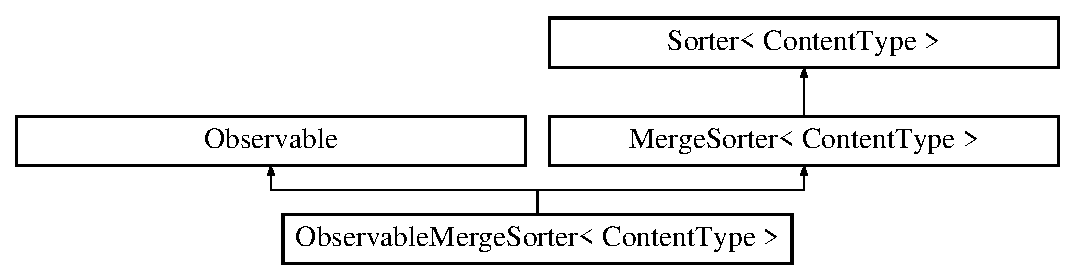
\includegraphics[height=2.886598cm]{class_observable_merge_sorter}
\end{center}
\end{figure}
\subsubsection*{Metody publiczne}
\begin{DoxyCompactItemize}
\item 
\hyperlink{class_observable_merge_sorter_af447c85bc1fcafd2d1e191968155023a}{Observable\-Merge\-Sorter} (\hyperlink{class_my_list}{My\-List}$<$ My\-List\-Element\-Type $>$ \&my\-List)
\item 
\hyperlink{class_list}{List}$<$ My\-List\-Element\-Type $>$ \& \hyperlink{class_observable_merge_sorter_ac845eed6758733f3935ffb5aa0b5f64a}{sort} ()
\begin{DoxyCompactList}\small\item\em sortuje przez scalanie \end{DoxyCompactList}\item 
virtual \hyperlink{class_observable_merge_sorter_a7d3a5f7257974ace9094cff9d499df99}{$\sim$\-Observable\-Merge\-Sorter} ()
\end{DoxyCompactItemize}
\subsubsection*{Dodatkowe Dziedziczone Składowe}


\subsubsection{Opis szczegółowy}
\subsubsection*{template$<$class My\-List\-Element\-Type$>$class Observable\-Merge\-Sorter$<$ My\-List\-Element\-Type $>$}



Definicja w linii \hyperlink{observablemergesorter_8h_source_l00018}{18} pliku \hyperlink{observablemergesorter_8h_source}{observablemergesorter.\-h}.



\subsubsection{Dokumentacja konstruktora i destruktora}
\hypertarget{class_observable_merge_sorter_af447c85bc1fcafd2d1e191968155023a}{\index{Observable\-Merge\-Sorter@{Observable\-Merge\-Sorter}!Observable\-Merge\-Sorter@{Observable\-Merge\-Sorter}}
\index{Observable\-Merge\-Sorter@{Observable\-Merge\-Sorter}!ObservableMergeSorter@{Observable\-Merge\-Sorter}}
\paragraph[{Observable\-Merge\-Sorter}]{\setlength{\rightskip}{0pt plus 5cm}template$<$class My\-List\-Element\-Type$>$ {\bf Observable\-Merge\-Sorter}$<$ My\-List\-Element\-Type $>$\-::{\bf Observable\-Merge\-Sorter} (
\begin{DoxyParamCaption}
\item[{{\bf My\-List}$<$ My\-List\-Element\-Type $>$ \&}]{my\-List}
\end{DoxyParamCaption}
)\hspace{0.3cm}{\ttfamily [inline]}}}\label{class_observable_merge_sorter_af447c85bc1fcafd2d1e191968155023a}


Definicja w linii \hyperlink{observablemergesorter_8h_source_l00021}{21} pliku \hyperlink{observablemergesorter_8h_source}{observablemergesorter.\-h}.


\begin{DoxyCode}
00021                                                                 :
00022                 \hyperlink{class_merge_sorter_a0ffb06429d7ebcb8bd007ca5db53429f}{MergeSorter<MyListElementType>::MergeSorter}(
      myList)\{\}
\end{DoxyCode}
\hypertarget{class_observable_merge_sorter_a7d3a5f7257974ace9094cff9d499df99}{\index{Observable\-Merge\-Sorter@{Observable\-Merge\-Sorter}!$\sim$\-Observable\-Merge\-Sorter@{$\sim$\-Observable\-Merge\-Sorter}}
\index{$\sim$\-Observable\-Merge\-Sorter@{$\sim$\-Observable\-Merge\-Sorter}!ObservableMergeSorter@{Observable\-Merge\-Sorter}}
\paragraph[{$\sim$\-Observable\-Merge\-Sorter}]{\setlength{\rightskip}{0pt plus 5cm}template$<$class My\-List\-Element\-Type$>$ virtual {\bf Observable\-Merge\-Sorter}$<$ My\-List\-Element\-Type $>$\-::$\sim${\bf Observable\-Merge\-Sorter} (
\begin{DoxyParamCaption}
{}
\end{DoxyParamCaption}
)\hspace{0.3cm}{\ttfamily [inline]}, {\ttfamily [virtual]}}}\label{class_observable_merge_sorter_a7d3a5f7257974ace9094cff9d499df99}


Definicja w linii \hyperlink{observablemergesorter_8h_source_l00033}{33} pliku \hyperlink{observablemergesorter_8h_source}{observablemergesorter.\-h}.


\begin{DoxyCode}
00033 \{\};
\end{DoxyCode}


\subsubsection{Dokumentacja funkcji składowych}
\hypertarget{class_observable_merge_sorter_ac845eed6758733f3935ffb5aa0b5f64a}{\index{Observable\-Merge\-Sorter@{Observable\-Merge\-Sorter}!sort@{sort}}
\index{sort@{sort}!ObservableMergeSorter@{Observable\-Merge\-Sorter}}
\paragraph[{sort}]{\setlength{\rightskip}{0pt plus 5cm}template$<$class My\-List\-Element\-Type$>$ {\bf List}$<$My\-List\-Element\-Type$>$\& {\bf Observable\-Merge\-Sorter}$<$ My\-List\-Element\-Type $>$\-::sort (
\begin{DoxyParamCaption}
{}
\end{DoxyParamCaption}
)\hspace{0.3cm}{\ttfamily [inline]}, {\ttfamily [virtual]}}}\label{class_observable_merge_sorter_ac845eed6758733f3935ffb5aa0b5f64a}


Reimplementowana z \hyperlink{class_merge_sorter_aaee4333eb37af6401eca60da3398e507}{Merge\-Sorter$<$ My\-List\-Element\-Type $>$}.



Definicja w linii \hyperlink{observablemergesorter_8h_source_l00026}{26} pliku \hyperlink{observablemergesorter_8h_source}{observablemergesorter.\-h}.



Odwołuje się do \hyperlink{mergesorter_8h_source_l00020}{Merge\-Sorter$<$ My\-List\-Element\-Type $>$\-::list}, \hyperlink{observable_8h_source_l00029}{Observable\-::send\-Start\-Update\-To\-Observers()}, \hyperlink{observable_8h_source_l00039}{Observable\-::send\-Stop\-Update\-To\-Observers()} i \hyperlink{mergesorter_8h_source_l00095}{Merge\-Sorter$<$ My\-List\-Element\-Type $>$\-::sort()}.



Odwołania w \hyperlink{main_8cpp_source_l00022}{main()}.


\begin{DoxyCode}
00027         \{
00028                 \hyperlink{class_observable_a78df64057f152342a43f27979186a6ba}{sendStartUpdateToObservers}();
00029                 \hyperlink{class_merge_sorter_aaee4333eb37af6401eca60da3398e507}{MergeSorter<MyListElementType>::sort}();
00030                 \hyperlink{class_observable_a16f75ed1514a0cb7526b5a5d2b7ca7c6}{sendStopUpdateToObservers}();
00031                 \textcolor{keywordflow}{return} this->\hyperlink{class_merge_sorter_a8ac3ee938414809d7da627cf918f1f87}{list};
00032         \}
\end{DoxyCode}


Dokumentacja dla tej klasy została wygenerowana z pliku\-:\begin{DoxyCompactItemize}
\item 
\hyperlink{observablemergesorter_8h}{observablemergesorter.\-h}\end{DoxyCompactItemize}

\hypertarget{class_observable_quick_sorter}{\subsection{Dokumentacja szablonu klasy Observable\-Quick\-Sorter$<$ My\-List\-Element\-Type $>$}
\label{class_observable_quick_sorter}\index{Observable\-Quick\-Sorter$<$ My\-List\-Element\-Type $>$@{Observable\-Quick\-Sorter$<$ My\-List\-Element\-Type $>$}}
}


Klasa sluzaca do obslugi sortowania przez Sortowanie szybkie z dodaniem obserwatora.  




{\ttfamily \#include $<$observablequicksorter.\-h$>$}

Diagram dziedziczenia dla Observable\-Quick\-Sorter$<$ My\-List\-Element\-Type $>$\begin{figure}[H]
\begin{center}
\leavevmode
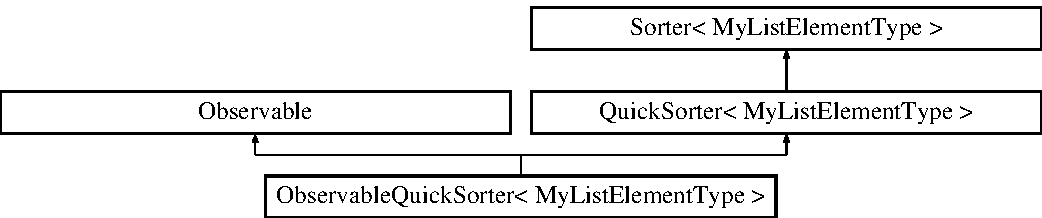
\includegraphics[height=2.926829cm]{class_observable_quick_sorter}
\end{center}
\end{figure}
\subsubsection*{Metody publiczne}
\begin{DoxyCompactItemize}
\item 
\hyperlink{class_observable_quick_sorter_a217751e25c07354b33d9e417bcc4f0c4}{Observable\-Quick\-Sorter} (\hyperlink{class_list}{List}$<$ My\-List\-Element\-Type $>$ \&\hyperlink{class_quick_sorter_a60a7a4772c958f256962294418e83fe4}{list})
\item 
\hyperlink{class_list}{List}$<$ My\-List\-Element\-Type $>$ \& \hyperlink{class_observable_quick_sorter_aa32fd1f6c024b3993c4d43302d0702f3}{sort} ()
\begin{DoxyCompactList}\small\item\em sortuje przez scalanie \end{DoxyCompactList}\item 
virtual \hyperlink{class_observable_quick_sorter_a346874659e31256462d9cf8caab53a6e}{$\sim$\-Observable\-Quick\-Sorter} ()
\end{DoxyCompactItemize}
\subsubsection*{Dodatkowe Dziedziczone Składowe}


\subsubsection{Opis szczegółowy}
\subsubsection*{template$<$class My\-List\-Element\-Type$>$class Observable\-Quick\-Sorter$<$ My\-List\-Element\-Type $>$}



Definicja w linii \hyperlink{observablequicksorter_8h_source_l00018}{18} pliku \hyperlink{observablequicksorter_8h_source}{observablequicksorter.\-h}.



\subsubsection{Dokumentacja konstruktora i destruktora}
\hypertarget{class_observable_quick_sorter_a217751e25c07354b33d9e417bcc4f0c4}{\index{Observable\-Quick\-Sorter@{Observable\-Quick\-Sorter}!Observable\-Quick\-Sorter@{Observable\-Quick\-Sorter}}
\index{Observable\-Quick\-Sorter@{Observable\-Quick\-Sorter}!ObservableQuickSorter@{Observable\-Quick\-Sorter}}
\paragraph[{Observable\-Quick\-Sorter}]{\setlength{\rightskip}{0pt plus 5cm}template$<$class My\-List\-Element\-Type$>$ {\bf Observable\-Quick\-Sorter}$<$ My\-List\-Element\-Type $>$\-::{\bf Observable\-Quick\-Sorter} (
\begin{DoxyParamCaption}
\item[{{\bf List}$<$ My\-List\-Element\-Type $>$ \&}]{list}
\end{DoxyParamCaption}
)\hspace{0.3cm}{\ttfamily [inline]}}}\label{class_observable_quick_sorter_a217751e25c07354b33d9e417bcc4f0c4}


Definicja w linii \hyperlink{observablequicksorter_8h_source_l00021}{21} pliku \hyperlink{observablequicksorter_8h_source}{observablequicksorter.\-h}.


\begin{DoxyCode}
00021                                                             :
00022                 \hyperlink{class_quick_sorter_a48497adf59b538717b4820721fd5d195}{QuickSorter<MyListElementType>::QuickSorter}(list
      )\{\}
\end{DoxyCode}
\hypertarget{class_observable_quick_sorter_a346874659e31256462d9cf8caab53a6e}{\index{Observable\-Quick\-Sorter@{Observable\-Quick\-Sorter}!$\sim$\-Observable\-Quick\-Sorter@{$\sim$\-Observable\-Quick\-Sorter}}
\index{$\sim$\-Observable\-Quick\-Sorter@{$\sim$\-Observable\-Quick\-Sorter}!ObservableQuickSorter@{Observable\-Quick\-Sorter}}
\paragraph[{$\sim$\-Observable\-Quick\-Sorter}]{\setlength{\rightskip}{0pt plus 5cm}template$<$class My\-List\-Element\-Type$>$ virtual {\bf Observable\-Quick\-Sorter}$<$ My\-List\-Element\-Type $>$\-::$\sim${\bf Observable\-Quick\-Sorter} (
\begin{DoxyParamCaption}
{}
\end{DoxyParamCaption}
)\hspace{0.3cm}{\ttfamily [inline]}, {\ttfamily [virtual]}}}\label{class_observable_quick_sorter_a346874659e31256462d9cf8caab53a6e}


Definicja w linii \hyperlink{observablequicksorter_8h_source_l00033}{33} pliku \hyperlink{observablequicksorter_8h_source}{observablequicksorter.\-h}.


\begin{DoxyCode}
00033 \{\};
\end{DoxyCode}


\subsubsection{Dokumentacja funkcji składowych}
\hypertarget{class_observable_quick_sorter_aa32fd1f6c024b3993c4d43302d0702f3}{\index{Observable\-Quick\-Sorter@{Observable\-Quick\-Sorter}!sort@{sort}}
\index{sort@{sort}!ObservableQuickSorter@{Observable\-Quick\-Sorter}}
\paragraph[{sort}]{\setlength{\rightskip}{0pt plus 5cm}template$<$class My\-List\-Element\-Type$>$ {\bf List}$<$My\-List\-Element\-Type$>$\& {\bf Observable\-Quick\-Sorter}$<$ My\-List\-Element\-Type $>$\-::sort (
\begin{DoxyParamCaption}
{}
\end{DoxyParamCaption}
)\hspace{0.3cm}{\ttfamily [inline]}, {\ttfamily [virtual]}}}\label{class_observable_quick_sorter_aa32fd1f6c024b3993c4d43302d0702f3}


Implementuje \hyperlink{class_sorter_a4a82d8151d6172802d1e60cb30c7d7d3}{Sorter$<$ My\-List\-Element\-Type $>$}.



Definicja w linii \hyperlink{observablequicksorter_8h_source_l00026}{26} pliku \hyperlink{observablequicksorter_8h_source}{observablequicksorter.\-h}.



Odwołuje się do \hyperlink{quicksorter_8h_source_l00023}{Quick\-Sorter$<$ My\-List\-Element\-Type $>$\-::list}, \hyperlink{observable_8h_source_l00029}{Observable\-::send\-Start\-Update\-To\-Observers()}, \hyperlink{observable_8h_source_l00039}{Observable\-::send\-Stop\-Update\-To\-Observers()} i \hyperlink{quicksorter_8h_source_l00069}{Quick\-Sorter$<$ My\-List\-Element\-Type $>$\-::sort()}.



Odwołania w \hyperlink{main_8cpp_source_l00022}{main()}.


\begin{DoxyCode}
00027         \{
00028                 \hyperlink{class_observable_a78df64057f152342a43f27979186a6ba}{sendStartUpdateToObservers}();
00029                 \hyperlink{class_quick_sorter_ae2b74900a972d05c06df3c9a06123c00}{QuickSorter<MyListElementType>::sort}();
00030                 \hyperlink{class_observable_a16f75ed1514a0cb7526b5a5d2b7ca7c6}{sendStopUpdateToObservers}();
00031                 \textcolor{keywordflow}{return} this->\hyperlink{class_quick_sorter_a60a7a4772c958f256962294418e83fe4}{list};
00032         \}
\end{DoxyCode}


Dokumentacja dla tej klasy została wygenerowana z pliku\-:\begin{DoxyCompactItemize}
\item 
\hyperlink{observablequicksorter_8h}{observablequicksorter.\-h}\end{DoxyCompactItemize}

\hypertarget{class_observer}{\subsection{Dokumentacja klasy Observer}
\label{class_observer}\index{Observer@{Observer}}
}


{\ttfamily \#include $<$observer.\-h$>$}

Diagram dziedziczenia dla Observer\begin{figure}[H]
\begin{center}
\leavevmode
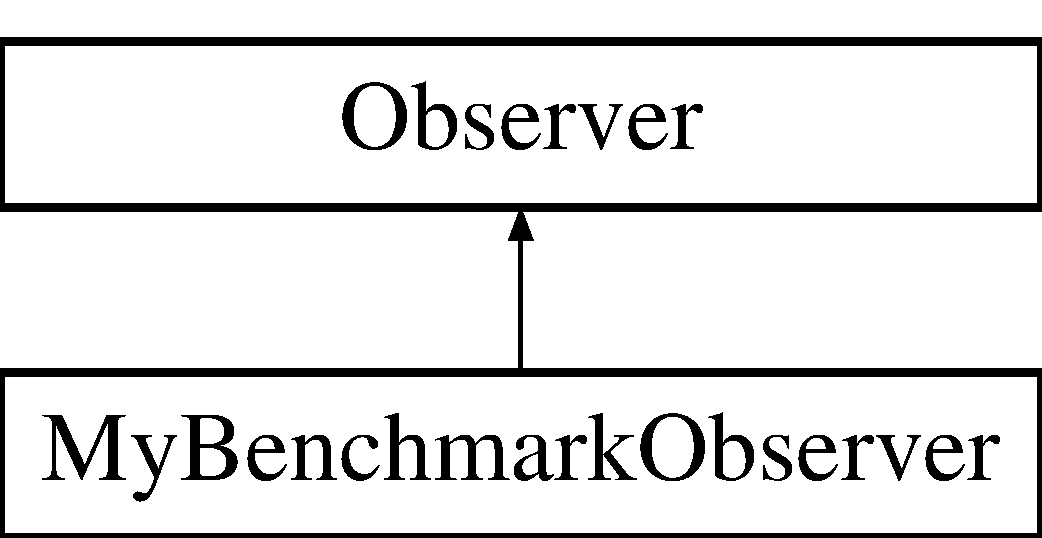
\includegraphics[height=2.000000cm]{class_observer}
\end{center}
\end{figure}
\subsubsection*{Metody publiczne}
\begin{DoxyCompactItemize}
\item 
virtual double \hyperlink{class_observer_a5ea7b52632401a92b7ba0aca5bceceaa}{get\-Timer\-Value} ()=0
\item 
virtual void \hyperlink{class_observer_a69ca89633f4624b79ec696a049793ba4}{received\-Start\-Update} ()=0
\item 
virtual void \hyperlink{class_observer_a8eb646ac3407c4d24d01178a6ba74f7f}{received\-Stop\-Update} ()=0
\item 
virtual void \hyperlink{class_observer_a764dd4568782b41271aa832edbe4455e}{received\-Stop\-Update\-And\-Save\-To\-File} ()=0
\item 
virtual \hyperlink{class_observer_afcc6b67be6c386f2f3d2c363aa59cb47}{$\sim$\-Observer} ()
\end{DoxyCompactItemize}


\subsubsection{Opis szczegółowy}


Definicja w linii \hyperlink{observer_8h_source_l00016}{16} pliku \hyperlink{observer_8h_source}{observer.\-h}.



\subsubsection{Dokumentacja konstruktora i destruktora}
\hypertarget{class_observer_afcc6b67be6c386f2f3d2c363aa59cb47}{\index{Observer@{Observer}!$\sim$\-Observer@{$\sim$\-Observer}}
\index{$\sim$\-Observer@{$\sim$\-Observer}!Observer@{Observer}}
\paragraph[{$\sim$\-Observer}]{\setlength{\rightskip}{0pt plus 5cm}virtual Observer\-::$\sim$\-Observer (
\begin{DoxyParamCaption}
{}
\end{DoxyParamCaption}
)\hspace{0.3cm}{\ttfamily [inline]}, {\ttfamily [virtual]}}}\label{class_observer_afcc6b67be6c386f2f3d2c363aa59cb47}


Definicja w linii \hyperlink{observer_8h_source_l00022}{22} pliku \hyperlink{observer_8h_source}{observer.\-h}.


\begin{DoxyCode}
00022 \{\};
\end{DoxyCode}


\subsubsection{Dokumentacja funkcji składowych}
\hypertarget{class_observer_a5ea7b52632401a92b7ba0aca5bceceaa}{\index{Observer@{Observer}!get\-Timer\-Value@{get\-Timer\-Value}}
\index{get\-Timer\-Value@{get\-Timer\-Value}!Observer@{Observer}}
\paragraph[{get\-Timer\-Value}]{\setlength{\rightskip}{0pt plus 5cm}virtual double Observer\-::get\-Timer\-Value (
\begin{DoxyParamCaption}
{}
\end{DoxyParamCaption}
)\hspace{0.3cm}{\ttfamily [pure virtual]}}}\label{class_observer_a5ea7b52632401a92b7ba0aca5bceceaa}


Implementowany w \hyperlink{class_my_benchmark_observer_a33ea57a2d321f835f3af0d3bab76a931}{My\-Benchmark\-Observer}.

\hypertarget{class_observer_a69ca89633f4624b79ec696a049793ba4}{\index{Observer@{Observer}!received\-Start\-Update@{received\-Start\-Update}}
\index{received\-Start\-Update@{received\-Start\-Update}!Observer@{Observer}}
\paragraph[{received\-Start\-Update}]{\setlength{\rightskip}{0pt plus 5cm}virtual void Observer\-::received\-Start\-Update (
\begin{DoxyParamCaption}
{}
\end{DoxyParamCaption}
)\hspace{0.3cm}{\ttfamily [pure virtual]}}}\label{class_observer_a69ca89633f4624b79ec696a049793ba4}


Implementowany w \hyperlink{class_my_benchmark_observer_a50a758f459b683b82bbb32fa4c2f13df}{My\-Benchmark\-Observer}.

\hypertarget{class_observer_a8eb646ac3407c4d24d01178a6ba74f7f}{\index{Observer@{Observer}!received\-Stop\-Update@{received\-Stop\-Update}}
\index{received\-Stop\-Update@{received\-Stop\-Update}!Observer@{Observer}}
\paragraph[{received\-Stop\-Update}]{\setlength{\rightskip}{0pt plus 5cm}virtual void Observer\-::received\-Stop\-Update (
\begin{DoxyParamCaption}
{}
\end{DoxyParamCaption}
)\hspace{0.3cm}{\ttfamily [pure virtual]}}}\label{class_observer_a8eb646ac3407c4d24d01178a6ba74f7f}


Implementowany w \hyperlink{class_my_benchmark_observer_aaf6a636ef6e8d8f8f8bc6d540e432246}{My\-Benchmark\-Observer}.

\hypertarget{class_observer_a764dd4568782b41271aa832edbe4455e}{\index{Observer@{Observer}!received\-Stop\-Update\-And\-Save\-To\-File@{received\-Stop\-Update\-And\-Save\-To\-File}}
\index{received\-Stop\-Update\-And\-Save\-To\-File@{received\-Stop\-Update\-And\-Save\-To\-File}!Observer@{Observer}}
\paragraph[{received\-Stop\-Update\-And\-Save\-To\-File}]{\setlength{\rightskip}{0pt plus 5cm}virtual void Observer\-::received\-Stop\-Update\-And\-Save\-To\-File (
\begin{DoxyParamCaption}
{}
\end{DoxyParamCaption}
)\hspace{0.3cm}{\ttfamily [pure virtual]}}}\label{class_observer_a764dd4568782b41271aa832edbe4455e}


Implementowany w \hyperlink{class_my_benchmark_observer_a2c12408a0f213a39d3419fd807f30968}{My\-Benchmark\-Observer}.



Dokumentacja dla tej klasy została wygenerowana z pliku\-:\begin{DoxyCompactItemize}
\item 
\hyperlink{observer_8h}{observer.\-h}\end{DoxyCompactItemize}

\hypertarget{class_quick_sorter}{\subsection{Dokumentacja szablonu klasy Quick\-Sorter$<$ Content\-Type $>$}
\label{class_quick_sorter}\index{Quick\-Sorter$<$ Content\-Type $>$@{Quick\-Sorter$<$ Content\-Type $>$}}
}


Klasa sluzaca do obslugi sortowania przez Scalanie.  




{\ttfamily \#include $<$quicksorter.\-h$>$}

Diagram dziedziczenia dla Quick\-Sorter$<$ Content\-Type $>$\begin{figure}[H]
\begin{center}
\leavevmode
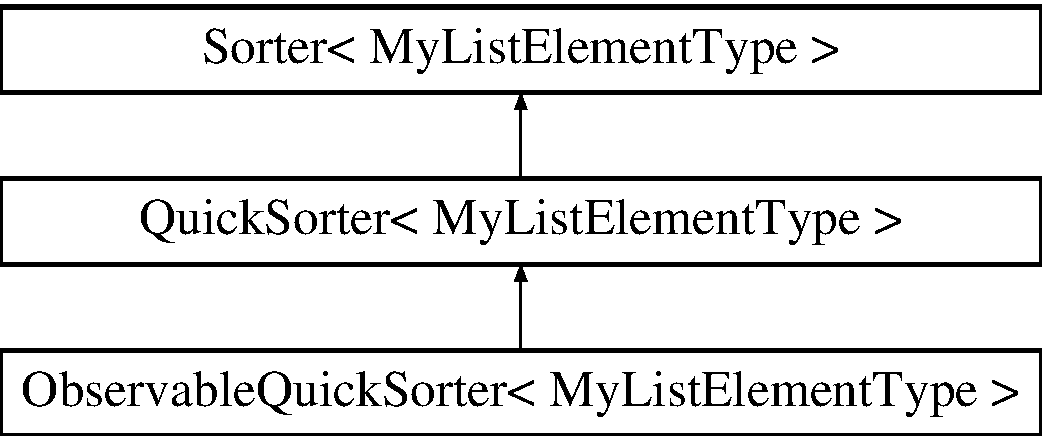
\includegraphics[height=3.000000cm]{class_quick_sorter}
\end{center}
\end{figure}
\subsubsection*{Metody publiczne}
\begin{DoxyCompactItemize}
\item 
\hyperlink{class_quick_sorter_a7a51572ed79a0c8e17bb4eb3f49a5a28}{Quick\-Sorter} (\hyperlink{class_list}{List}$<$ Content\-Type $>$ \&\hyperlink{class_quick_sorter_a66cd768b6d8a77952f004be7aad87a0e}{list})
\begin{DoxyCompactList}\small\item\em Konstruktor. \end{DoxyCompactList}\item 
virtual \hyperlink{class_quick_sorter_a485f3a798961c95288d6ca911615042e}{$\sim$\-Quick\-Sorter} ()
\item 
void \hyperlink{class_quick_sorter_a99641193667f65f8a203b65fdc0b4d92}{quicksort} (int lewy, int prawy)
\begin{DoxyCompactList}\small\item\em Szuka liczb do porownaia z pivotem. \end{DoxyCompactList}\item 
\hyperlink{class_list}{List}$<$ Content\-Type $>$ \& \hyperlink{class_quick_sorter_a86cadfe5f5b9fbdf6e9eacb0b7dbc83d}{sort} ()
\begin{DoxyCompactList}\small\item\em Sortuje przez Sortowanie szybkie. \end{DoxyCompactList}\end{DoxyCompactItemize}
\subsubsection*{Atrybuty publiczne}
\begin{DoxyCompactItemize}
\item 
int \hyperlink{class_quick_sorter_a8c3f6118075353547d6fc5da57e2267e}{enable\-Pivot}
\item 
\hyperlink{class_list}{List}$<$ Content\-Type $>$ \& \hyperlink{class_quick_sorter_a66cd768b6d8a77952f004be7aad87a0e}{list}
\begin{DoxyCompactList}\small\item\em Skopiowana lista do przeprowadzania sortowania. \end{DoxyCompactList}\end{DoxyCompactItemize}


\subsubsection{Opis szczegółowy}
\subsubsection*{template$<$class Content\-Type$>$class Quick\-Sorter$<$ Content\-Type $>$}



Definicja w linii \hyperlink{quicksorter_8h_source_l00018}{18} pliku \hyperlink{quicksorter_8h_source}{quicksorter.\-h}.



\subsubsection{Dokumentacja konstruktora i destruktora}
\hypertarget{class_quick_sorter_a7a51572ed79a0c8e17bb4eb3f49a5a28}{\index{Quick\-Sorter@{Quick\-Sorter}!Quick\-Sorter@{Quick\-Sorter}}
\index{Quick\-Sorter@{Quick\-Sorter}!QuickSorter@{Quick\-Sorter}}
\paragraph[{Quick\-Sorter}]{\setlength{\rightskip}{0pt plus 5cm}template$<$class Content\-Type $>$ {\bf Quick\-Sorter}$<$ Content\-Type $>$\-::{\bf Quick\-Sorter} (
\begin{DoxyParamCaption}
\item[{{\bf List}$<$ Content\-Type $>$ \&}]{list}
\end{DoxyParamCaption}
)\hspace{0.3cm}{\ttfamily [inline]}}}\label{class_quick_sorter_a7a51572ed79a0c8e17bb4eb3f49a5a28}

\begin{DoxyParams}{Parametry}
{\em \&list} & lista, która konstruktor kopiuje aby nie naruszać podanej przez uzytkownika \\
\hline
\end{DoxyParams}


Definicja w linii \hyperlink{quicksorter_8h_source_l00028}{28} pliku \hyperlink{quicksorter_8h_source}{quicksorter.\-h}.



Odwołuje się do \hyperlink{list_8h_source_l00068}{List$<$ Content\-Type $>$\-::clone\-From()} i \hyperlink{quicksorter_8h_source_l00021}{Quick\-Sorter$<$ Content\-Type $>$\-::enable\-Pivot}.


\begin{DoxyCode}
00029         :\hyperlink{class_quick_sorter_a66cd768b6d8a77952f004be7aad87a0e}{list}(list.\hyperlink{class_list_a87870a63c8d7bb7530356d9278e766a9}{createObjectFromAbstractReference}())
00030         \{
00031                 this->list.\hyperlink{class_list_a8a1ebc7ce83d77b83f58bd8c2ce2d683}{cloneFrom}(list);
00032                 this->\hyperlink{class_quick_sorter_a8c3f6118075353547d6fc5da57e2267e}{enablePivot}=1;
00033         \}
\end{DoxyCode}
\hypertarget{class_quick_sorter_a485f3a798961c95288d6ca911615042e}{\index{Quick\-Sorter@{Quick\-Sorter}!$\sim$\-Quick\-Sorter@{$\sim$\-Quick\-Sorter}}
\index{$\sim$\-Quick\-Sorter@{$\sim$\-Quick\-Sorter}!QuickSorter@{Quick\-Sorter}}
\paragraph[{$\sim$\-Quick\-Sorter}]{\setlength{\rightskip}{0pt plus 5cm}template$<$class Content\-Type $>$ virtual {\bf Quick\-Sorter}$<$ Content\-Type $>$\-::$\sim${\bf Quick\-Sorter} (
\begin{DoxyParamCaption}
{}
\end{DoxyParamCaption}
)\hspace{0.3cm}{\ttfamily [inline]}, {\ttfamily [virtual]}}}\label{class_quick_sorter_a485f3a798961c95288d6ca911615042e}


Definicja w linii \hyperlink{quicksorter_8h_source_l00035}{35} pliku \hyperlink{quicksorter_8h_source}{quicksorter.\-h}.


\begin{DoxyCode}
00035 \{\};
\end{DoxyCode}


\subsubsection{Dokumentacja funkcji składowych}
\hypertarget{class_quick_sorter_a99641193667f65f8a203b65fdc0b4d92}{\index{Quick\-Sorter@{Quick\-Sorter}!quicksort@{quicksort}}
\index{quicksort@{quicksort}!QuickSorter@{Quick\-Sorter}}
\paragraph[{quicksort}]{\setlength{\rightskip}{0pt plus 5cm}template$<$class Content\-Type $>$ void {\bf Quick\-Sorter}$<$ Content\-Type $>$\-::quicksort (
\begin{DoxyParamCaption}
\item[{int}]{lewy, }
\item[{int}]{prawy}
\end{DoxyParamCaption}
)\hspace{0.3cm}{\ttfamily [inline]}}}\label{class_quick_sorter_a99641193667f65f8a203b65fdc0b4d92}

\begin{DoxyParams}{Parametry}
{\em lewy} & brzeg poszukiwan \\
\hline
{\em prawy} & brzeg poszukiwan \\
\hline
\end{DoxyParams}


Definicja w linii \hyperlink{quicksorter_8h_source_l00042}{42} pliku \hyperlink{quicksorter_8h_source}{quicksorter.\-h}.



Odwołuje się do \hyperlink{quicksorter_8h_source_l00021}{Quick\-Sorter$<$ Content\-Type $>$\-::enable\-Pivot} i \hyperlink{quicksorter_8h_source_l00023}{Quick\-Sorter$<$ Content\-Type $>$\-::list}.



Odwołania w \hyperlink{quicksorter_8h_source_l00067}{Quick\-Sorter$<$ Content\-Type $>$\-::sort()}.


\begin{DoxyCode}
00043         \{
00044             \textcolor{keywordtype}{int} pivot=\hyperlink{class_quick_sorter_a66cd768b6d8a77952f004be7aad87a0e}{list}[(int)(lewy+prawy)/2];
00045             \textcolor{keywordtype}{int} i=lewy,j=prawy, x;
00046             \textcolor{keywordflow}{if}(\hyperlink{class_quick_sorter_a8c3f6118075353547d6fc5da57e2267e}{enablePivot}) pivot=(\hyperlink{class_quick_sorter_a66cd768b6d8a77952f004be7aad87a0e}{list}[(int)(lewy+prawy)/2] + 
      \hyperlink{class_quick_sorter_a66cd768b6d8a77952f004be7aad87a0e}{list}[lewy] + \hyperlink{class_quick_sorter_a66cd768b6d8a77952f004be7aad87a0e}{list}[prawy])/3;
00047             \textcolor{keywordflow}{do}
00048             \{
00049                 \textcolor{keywordflow}{while}(\hyperlink{class_quick_sorter_a66cd768b6d8a77952f004be7aad87a0e}{list}[i]<pivot) \{i++; \}
00050                 \textcolor{keywordflow}{while}(\hyperlink{class_quick_sorter_a66cd768b6d8a77952f004be7aad87a0e}{list}[j]>pivot) \{j--; \}
00051                 \textcolor{keywordflow}{if}(i<=j)
00052                 \{
00053                         x =\hyperlink{class_quick_sorter_a66cd768b6d8a77952f004be7aad87a0e}{list}[i];
00054                     \hyperlink{class_quick_sorter_a66cd768b6d8a77952f004be7aad87a0e}{list}[i]=\hyperlink{class_quick_sorter_a66cd768b6d8a77952f004be7aad87a0e}{list}[j];
00055                     \hyperlink{class_quick_sorter_a66cd768b6d8a77952f004be7aad87a0e}{list}[j]=x;
00056                     i++;
00057                     j--;
00058                 \}
00059             \}
00060             \textcolor{keywordflow}{while}(i<=j);
00061             \textcolor{keywordflow}{if}(j>lewy) \hyperlink{class_quick_sorter_a99641193667f65f8a203b65fdc0b4d92}{quicksort}(lewy, j);
00062             \textcolor{keywordflow}{if}(i<prawy) \hyperlink{class_quick_sorter_a99641193667f65f8a203b65fdc0b4d92}{quicksort}(i, prawy);
00063         \}
\end{DoxyCode}
\hypertarget{class_quick_sorter_a86cadfe5f5b9fbdf6e9eacb0b7dbc83d}{\index{Quick\-Sorter@{Quick\-Sorter}!sort@{sort}}
\index{sort@{sort}!QuickSorter@{Quick\-Sorter}}
\paragraph[{sort}]{\setlength{\rightskip}{0pt plus 5cm}template$<$class Content\-Type $>$ {\bf List}$<$Content\-Type$>$\& {\bf Quick\-Sorter}$<$ Content\-Type $>$\-::sort (
\begin{DoxyParamCaption}
{}
\end{DoxyParamCaption}
)\hspace{0.3cm}{\ttfamily [inline]}, {\ttfamily [virtual]}}}\label{class_quick_sorter_a86cadfe5f5b9fbdf6e9eacb0b7dbc83d}


Implementuje \hyperlink{class_sorter_a880cfd8969b78557ed207ad6f2bd4819}{Sorter$<$ Content\-Type $>$}.



Definicja w linii \hyperlink{quicksorter_8h_source_l00067}{67} pliku \hyperlink{quicksorter_8h_source}{quicksorter.\-h}.



Odwołuje się do \hyperlink{quicksorter_8h_source_l00023}{Quick\-Sorter$<$ Content\-Type $>$\-::list} i \hyperlink{quicksorter_8h_source_l00042}{Quick\-Sorter$<$ Content\-Type $>$\-::quicksort()}.



Odwołania w \hyperlink{observablequicksorter_8h_source_l00026}{Observable\-Quick\-Sorter$<$ Content\-Type $>$\-::sort()}.


\begin{DoxyCode}
00068         \{
00069                 \textcolor{comment}{//std::cout<<"(QuickSort)";}
00070                 \hyperlink{class_quick_sorter_a99641193667f65f8a203b65fdc0b4d92}{quicksort}(0, \hyperlink{class_quick_sorter_a66cd768b6d8a77952f004be7aad87a0e}{list}.size()-1);
00071                 \textcolor{keywordflow}{return} \hyperlink{class_quick_sorter_a66cd768b6d8a77952f004be7aad87a0e}{list};
00072         \}
\end{DoxyCode}


\subsubsection{Dokumentacja atrybutów składowych}
\hypertarget{class_quick_sorter_a8c3f6118075353547d6fc5da57e2267e}{\index{Quick\-Sorter@{Quick\-Sorter}!enable\-Pivot@{enable\-Pivot}}
\index{enable\-Pivot@{enable\-Pivot}!QuickSorter@{Quick\-Sorter}}
\paragraph[{enable\-Pivot}]{\setlength{\rightskip}{0pt plus 5cm}template$<$class Content\-Type $>$ int {\bf Quick\-Sorter}$<$ Content\-Type $>$\-::enable\-Pivot}}\label{class_quick_sorter_a8c3f6118075353547d6fc5da57e2267e}


Definicja w linii \hyperlink{quicksorter_8h_source_l00021}{21} pliku \hyperlink{quicksorter_8h_source}{quicksorter.\-h}.



Odwołania w \hyperlink{quicksorter_8h_source_l00042}{Quick\-Sorter$<$ Content\-Type $>$\-::quicksort()} i \hyperlink{quicksorter_8h_source_l00028}{Quick\-Sorter$<$ Content\-Type $>$\-::\-Quick\-Sorter()}.

\hypertarget{class_quick_sorter_a66cd768b6d8a77952f004be7aad87a0e}{\index{Quick\-Sorter@{Quick\-Sorter}!list@{list}}
\index{list@{list}!QuickSorter@{Quick\-Sorter}}
\paragraph[{list}]{\setlength{\rightskip}{0pt plus 5cm}template$<$class Content\-Type $>$ {\bf List}$<$Content\-Type$>$\& {\bf Quick\-Sorter}$<$ Content\-Type $>$\-::list}}\label{class_quick_sorter_a66cd768b6d8a77952f004be7aad87a0e}


Definicja w linii \hyperlink{quicksorter_8h_source_l00023}{23} pliku \hyperlink{quicksorter_8h_source}{quicksorter.\-h}.



Odwołania w \hyperlink{main_8cpp_source_l00022}{main()}, \hyperlink{quicksorter_8h_source_l00042}{Quick\-Sorter$<$ Content\-Type $>$\-::quicksort()}, \hyperlink{observablequicksorter_8h_source_l00026}{Observable\-Quick\-Sorter$<$ Content\-Type $>$\-::sort()} i \hyperlink{quicksorter_8h_source_l00067}{Quick\-Sorter$<$ Content\-Type $>$\-::sort()}.



Dokumentacja dla tej klasy została wygenerowana z pliku\-:\begin{DoxyCompactItemize}
\item 
\hyperlink{quicksorter_8h}{quicksorter.\-h}\end{DoxyCompactItemize}

\hypertarget{class_sorter}{\subsection{Dokumentacja szablonu klasy Sorter$<$ My\-List\-Element\-Type $>$}
\label{class_sorter}\index{Sorter$<$ My\-List\-Element\-Type $>$@{Sorter$<$ My\-List\-Element\-Type $>$}}
}


{\ttfamily \#include $<$sorter.\-h$>$}

Diagram dziedziczenia dla Sorter$<$ My\-List\-Element\-Type $>$\begin{figure}[H]
\begin{center}
\leavevmode
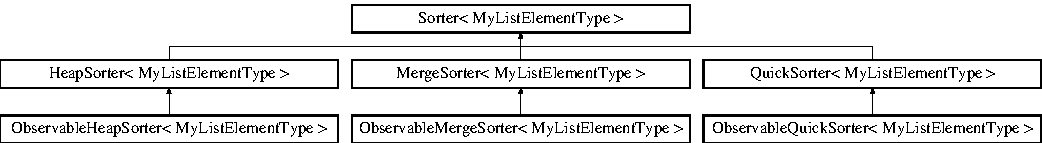
\includegraphics[height=1.924399cm]{class_sorter}
\end{center}
\end{figure}
\subsubsection*{Metody publiczne}
\begin{DoxyCompactItemize}
\item 
virtual \hyperlink{class_list}{List}$<$ My\-List\-Element\-Type $>$ \& \hyperlink{class_sorter_a4a82d8151d6172802d1e60cb30c7d7d3}{sort} ()=0
\item 
virtual \hyperlink{class_sorter_ac71eebbce06b3fa6a3280c5733d999a5}{$\sim$\-Sorter} ()
\end{DoxyCompactItemize}


\subsubsection{Opis szczegółowy}
\subsubsection*{template$<$class My\-List\-Element\-Type$>$class Sorter$<$ My\-List\-Element\-Type $>$}



Definicja w linii \hyperlink{sorter_8h_source_l00015}{15} pliku \hyperlink{sorter_8h_source}{sorter.\-h}.



\subsubsection{Dokumentacja konstruktora i destruktora}
\hypertarget{class_sorter_ac71eebbce06b3fa6a3280c5733d999a5}{\index{Sorter@{Sorter}!$\sim$\-Sorter@{$\sim$\-Sorter}}
\index{$\sim$\-Sorter@{$\sim$\-Sorter}!Sorter@{Sorter}}
\paragraph[{$\sim$\-Sorter}]{\setlength{\rightskip}{0pt plus 5cm}template$<$class My\-List\-Element\-Type $>$ virtual {\bf Sorter}$<$ My\-List\-Element\-Type $>$\-::$\sim${\bf Sorter} (
\begin{DoxyParamCaption}
{}
\end{DoxyParamCaption}
)\hspace{0.3cm}{\ttfamily [inline]}, {\ttfamily [virtual]}}}\label{class_sorter_ac71eebbce06b3fa6a3280c5733d999a5}


Definicja w linii \hyperlink{sorter_8h_source_l00020}{20} pliku \hyperlink{sorter_8h_source}{sorter.\-h}.


\begin{DoxyCode}
00020 \{\};
\end{DoxyCode}


\subsubsection{Dokumentacja funkcji składowych}
\hypertarget{class_sorter_a4a82d8151d6172802d1e60cb30c7d7d3}{\index{Sorter@{Sorter}!sort@{sort}}
\index{sort@{sort}!Sorter@{Sorter}}
\paragraph[{sort}]{\setlength{\rightskip}{0pt plus 5cm}template$<$class My\-List\-Element\-Type $>$ virtual {\bf List}$<$My\-List\-Element\-Type$>$\& {\bf Sorter}$<$ My\-List\-Element\-Type $>$\-::sort (
\begin{DoxyParamCaption}
{}
\end{DoxyParamCaption}
)\hspace{0.3cm}{\ttfamily [pure virtual]}}}\label{class_sorter_a4a82d8151d6172802d1e60cb30c7d7d3}


Implementowany w \hyperlink{class_merge_sorter_aaee4333eb37af6401eca60da3398e507}{Merge\-Sorter$<$ My\-List\-Element\-Type $>$}, \hyperlink{class_quick_sorter_ae2b74900a972d05c06df3c9a06123c00}{Quick\-Sorter$<$ My\-List\-Element\-Type $>$}, \hyperlink{class_heap_sorter_a31220ba55d4478c50578c3a94dcbf26c}{Heap\-Sorter$<$ My\-List\-Element\-Type $>$}, \hyperlink{class_observable_heap_sorter_a5e92d70e5a769ba7249f974a48b94bd0}{Observable\-Heap\-Sorter$<$ My\-List\-Element\-Type $>$}, \hyperlink{class_observable_merge_sorter_ac845eed6758733f3935ffb5aa0b5f64a}{Observable\-Merge\-Sorter$<$ My\-List\-Element\-Type $>$} i \hyperlink{class_observable_quick_sorter_aa32fd1f6c024b3993c4d43302d0702f3}{Observable\-Quick\-Sorter$<$ My\-List\-Element\-Type $>$}.



Dokumentacja dla tej klasy została wygenerowana z pliku\-:\begin{DoxyCompactItemize}
\item 
\hyperlink{sorter_8h}{sorter.\-h}\end{DoxyCompactItemize}

\section{Dokumentacja plików}
\hypertarget{bfs_8h}{\subsection{Dokumentacja pliku bfs.\-h}
\label{bfs_8h}\index{bfs.\-h@{bfs.\-h}}
}
{\ttfamily \#include $<$iostream$>$}\\*
{\ttfamily \#include \char`\"{}linkedlist.\-h\char`\"{}}\\*
{\ttfamily \#include \char`\"{}graph.\-h\char`\"{}}\\*
\subsubsection*{Komponenty}
\begin{DoxyCompactItemize}
\item 
class \hyperlink{class_b_f_s}{B\-F\-S}
\end{DoxyCompactItemize}
\subsubsection*{Definicje}
\begin{DoxyCompactItemize}
\item 
\#define \hyperlink{bfs_8h_a392fb874e547e582e9c66a08a1f23326}{M\-A\-X}~128
\end{DoxyCompactItemize}


\subsubsection{Dokumentacja definicji}
\hypertarget{bfs_8h_a392fb874e547e582e9c66a08a1f23326}{\index{bfs.\-h@{bfs.\-h}!M\-A\-X@{M\-A\-X}}
\index{M\-A\-X@{M\-A\-X}!bfs.h@{bfs.\-h}}
\paragraph[{M\-A\-X}]{\setlength{\rightskip}{0pt plus 5cm}\#define M\-A\-X~128}}\label{bfs_8h_a392fb874e547e582e9c66a08a1f23326}


Definicja w linii \hyperlink{bfs_8h_source_l00014}{14} pliku \hyperlink{bfs_8h_source}{bfs.\-h}.



Odwołania w \hyperlink{bfs_8h_source_l00068}{B\-F\-S\-::clean()}.


\hypertarget{bfs_8h}{\subsection{bfs.\-h}
\label{bfs_8h}\index{bfs.\-h@{bfs.\-h}}
}

\begin{DoxyCode}
00001 \textcolor{comment}{/*}
00002 \textcolor{comment}{ * bsf.h}
00003 \textcolor{comment}{ *}
00004 \textcolor{comment}{ *  Created on: May 28, 2015}
00005 \textcolor{comment}{ *      Author: serek8}
00006 \textcolor{comment}{ */}
00007 
00008 \textcolor{preprocessor}{#ifndef BSF\_H\_}
00009 \textcolor{preprocessor}{}\textcolor{preprocessor}{#define BSF\_H\_}
00010 \textcolor{preprocessor}{}
00011 \textcolor{preprocessor}{#include <iostream>}
00012 \textcolor{preprocessor}{#include "\hyperlink{linkedlist_8h}{linkedlist.h}"}
00013 \textcolor{preprocessor}{#include "\hyperlink{graph_8h}{graph.h}"}
\hypertarget{bfs_8h_source_l00014}{}\hyperlink{bfs_8h_a392fb874e547e582e9c66a08a1f23326}{00014} \textcolor{preprocessor}{#define MAX 128}
00015 \textcolor{preprocessor}{}
00016 \textcolor{keyword}{using namespace }std;
00017 
\hypertarget{bfs_8h_source_l00018}{}\hyperlink{class_b_f_s}{00018} \textcolor{keyword}{class }\hyperlink{class_b_f_s}{BFS} : \textcolor{keyword}{public} \hyperlink{class_graph}{Graph}
00019 \{
00020 \textcolor{keyword}{public}:
\hypertarget{bfs_8h_source_l00021}{}\hyperlink{class_b_f_s_a1191eb3076bf8f3f412cc68563c0b46f}{00021}         \textcolor{keywordtype}{int} pi[\hyperlink{bfs_8h_a392fb874e547e582e9c66a08a1f23326}{MAX}];       
\hypertarget{bfs_8h_source_l00022}{}\hyperlink{class_b_f_s_a317da6453a9b8e73f62e2bc60e9894fa}{00022}     \hyperlink{class_linked_list}{LinkedList<int>} \hyperlink{class_b_f_s_a317da6453a9b8e73f62e2bc60e9894fa}{q};  
00023 
\hypertarget{bfs_8h_source_l00024}{}\hyperlink{class_b_f_s_ae2f1a5dc47c9791ad2d90e40e812d229}{00024}     \hyperlink{class_b_f_s_ae2f1a5dc47c9791ad2d90e40e812d229}{BFS}()
00025     \{
00026                 clean();
00027     \}
\hypertarget{bfs_8h_source_l00028}{}\hyperlink{class_b_f_s_af70cee98b79886431c5d3f451d78f712}{00028}     \textcolor{keyword}{virtual} \hyperlink{class_b_f_s_af70cee98b79886431c5d3f451d78f712}{~BFS}()   \{        \}
00029 
\hypertarget{bfs_8h_source_l00030}{}\hyperlink{class_b_f_s_a392b91df16399ab3be7e3745379d9dc0}{00030}     \textcolor{keywordtype}{void} \hyperlink{class_b_f_s_a392b91df16399ab3be7e3745379d9dc0}{bfs}(\textcolor{keywordtype}{int} fromNumber, \textcolor{keywordtype}{int} toNumber)
00031     \{
00032         colour[fromNumber] = 1;
00033         pi[fromNumber]     = 1; \textcolor{comment}{// czyli brak rodzica}
00034         q.push\_back( fromNumber );
00035         \textcolor{keywordflow}{while} ( q.size() ) \{
00036                 \textcolor{keywordtype}{int} u = q[0];
00037                 q.pop\_front();
00038                 \textcolor{keywordflow}{for}( \textcolor{keywordtype}{int} v = 0; v < biggestValue; v++ ) \{
00039                         \textcolor{comment}{//cout<<"(test) colour:"<<colour[v]<<"\(\backslash\)t"<<M[u][v]<<endl;}
00040                         \textcolor{keywordflow}{if}( colour[v] == 0 && M[u][v] ) \{
00041                                 colour[v] = 1;
00042                                 pi[v] = u;         \textcolor{comment}{// zapisuje gdzie znajduje sie rodzic danej liczby}
00043                                 \textcolor{keywordflow}{if}(toNumber == v) \textcolor{keywordflow}{return};
00044                                 q.push\_back( v );
00045                         \}
00046                 \}
00047                 colour[u] = 2;
00048         \}
00049     \}
00050 
\hypertarget{bfs_8h_source_l00051}{}\hyperlink{class_b_f_s_a42789813e256a0225a26cf418c7754a2}{00051}     \textcolor{keywordtype}{void} \hyperlink{class_b_f_s_a42789813e256a0225a26cf418c7754a2}{findShortestPath}(\textcolor{keywordtype}{int} fromNumber, \textcolor{keywordtype}{int} toNumber)
00052     \{
00053         \hyperlink{class_linked_list}{LinkedList<int>} listaDoZmianyKolejnosci;
00054         \textcolor{keywordtype}{int} tmp=toNumber;
00055         bfs(fromNumber, toNumber);
00056         listaDoZmianyKolejnosci.\hyperlink{class_linked_list_a9effa3698ad28e2f3401cd199f852e08}{push\_front}(toNumber);
00057         \textcolor{keywordflow}{while}(1)
00058         \{
00059                 listaDoZmianyKolejnosci.\hyperlink{class_linked_list_a9effa3698ad28e2f3401cd199f852e08}{push\_front}(pi[tmp]);
00060                 tmp = pi[tmp];
00061                 \textcolor{keywordflow}{if}(tmp == fromNumber) \textcolor{keywordflow}{break};
00062         \}
00063         listaDoZmianyKolejnosci.\hyperlink{class_linked_list_a245ba50906c85c1765a5f611d3f3b6c0}{print}();
00064     \}
00065 
00066 
00067 
\hypertarget{bfs_8h_source_l00068}{}\hyperlink{class_b_f_s_a5d7b36488122996dc5877cd611afcaef}{00068}     \textcolor{keywordtype}{void} \hyperlink{class_b_f_s_a5d7b36488122996dc5877cd611afcaef}{clean}()
00069     \{
00070         num = 0;
00071         biggestValue = 0;
00072         \textcolor{keywordflow}{for} (\textcolor{keywordtype}{int} i = 0; i < \hyperlink{bfs_8h_a392fb874e547e582e9c66a08a1f23326}{MAX}; i++)
00073         \{
00074                 \textcolor{keywordflow}{for} (\textcolor{keywordtype}{int} j = 0; j < \hyperlink{bfs_8h_a392fb874e547e582e9c66a08a1f23326}{MAX}; j++)        M[i][j] = 0;
00075 
00076                 colour[i] = 0;    \textcolor{comment}{// ustawia numery jako biale}
00077                 pi[i] = 1;   \textcolor{comment}{// ustawia rodzicow na 1}
00078 
00079         \}
00080     \}
00081 \};
00082 
00083 \textcolor{preprocessor}{#endif }\textcolor{comment}{/* BSF\_H\_ */}\textcolor{preprocessor}{}
\end{DoxyCode}

\hypertarget{dfs_8h}{\subsection{Dokumentacja pliku dfs.\-h}
\label{dfs_8h}\index{dfs.\-h@{dfs.\-h}}
}
{\ttfamily \#include $<$iostream$>$}\\*
{\ttfamily \#include \char`\"{}linkedlist.\-h\char`\"{}}\\*
{\ttfamily \#include \char`\"{}graph.\-h\char`\"{}}\\*
\subsubsection*{Komponenty}
\begin{DoxyCompactItemize}
\item 
class \hyperlink{class_d_f_s}{D\-F\-S}
\begin{DoxyCompactList}\small\item\em Klasa przedstawia przeszukiwanie grafu za pomocą \hyperlink{class_d_f_s}{D\-F\-S} Umożliwia wyszukanie najkrótszej trasy do numeru. \end{DoxyCompactList}\end{DoxyCompactItemize}
\subsubsection*{Definicje}
\begin{DoxyCompactItemize}
\item 
\#define \hyperlink{dfs_8h_a392fb874e547e582e9c66a08a1f23326}{M\-A\-X}~128
\end{DoxyCompactItemize}


\subsubsection{Dokumentacja definicji}
\hypertarget{dfs_8h_a392fb874e547e582e9c66a08a1f23326}{\index{dfs.\-h@{dfs.\-h}!M\-A\-X@{M\-A\-X}}
\index{M\-A\-X@{M\-A\-X}!dfs.h@{dfs.\-h}}
\paragraph[{M\-A\-X}]{\setlength{\rightskip}{0pt plus 5cm}\#define M\-A\-X~128}}\label{dfs_8h_a392fb874e547e582e9c66a08a1f23326}


Definicja w linii \hyperlink{dfs_8h_source_l00014}{14} pliku \hyperlink{dfs_8h_source}{dfs.\-h}.



Odwołania w \hyperlink{dfs_8h_source_l00096}{D\-F\-S\-::clean()}.


\hypertarget{dfs_8h}{\subsection{dfs.\-h}
\label{dfs_8h}\index{dfs.\-h@{dfs.\-h}}
}

\begin{DoxyCode}
00001 \textcolor{comment}{/*}
00002 \textcolor{comment}{ * dfs.h}
00003 \textcolor{comment}{ *}
00004 \textcolor{comment}{ *  Created on: May 28, 2015}
00005 \textcolor{comment}{ *      Author: serek8}
00006 \textcolor{comment}{ */}
00007 
00008 \textcolor{preprocessor}{#ifndef DFS\_H\_}
00009 \textcolor{preprocessor}{}\textcolor{preprocessor}{#define DFS\_H\_}
00010 \textcolor{preprocessor}{}
00011 \textcolor{preprocessor}{#include <iostream>}
00012 \textcolor{preprocessor}{#include "\hyperlink{linkedlist_8h}{linkedlist.h}"}
00013 \textcolor{preprocessor}{#include "\hyperlink{graph_8h}{graph.h}"}
\hypertarget{dfs_8h_source_l00014}{}\hyperlink{dfs_8h_a392fb874e547e582e9c66a08a1f23326}{00014} \textcolor{preprocessor}{#define MAX 128}
00015 \textcolor{preprocessor}{}
00016 \textcolor{keyword}{using namespace }std;
00017 
\hypertarget{dfs_8h_source_l00022}{}\hyperlink{class_d_f_s}{00022} \textcolor{keyword}{class }\hyperlink{class_d_f_s}{DFS}:\textcolor{keyword}{public} \hyperlink{class_graph}{Graph}
00023 \{
00024 \textcolor{keyword}{public}:
\hypertarget{dfs_8h_source_l00025}{}\hyperlink{class_d_f_s_aa3bf5c11cd2d66fc893e232eb1e42c76}{00025}   \hyperlink{class_linked_list}{LinkedList<int>} \hyperlink{class_d_f_s_aa3bf5c11cd2d66fc893e232eb1e42c76}{currentPath};        
\hypertarget{dfs_8h_source_l00026}{}\hyperlink{class_d_f_s_a48dd546aaa57234bcd6e54a0f01b3f48}{00026}   \hyperlink{class_linked_list}{LinkedList<int>} allPaths[\hyperlink{dfs_8h_a392fb874e547e582e9c66a08a1f23326}{MAX}]; 
\hypertarget{dfs_8h_source_l00027}{}\hyperlink{class_d_f_s_a53269340075995e432c355638ce30554}{00027}   \textcolor{keywordtype}{int} \hyperlink{class_d_f_s_a53269340075995e432c355638ce30554}{allPathsAmount};     
00028 
\hypertarget{dfs_8h_source_l00029}{}\hyperlink{class_d_f_s_a75b2f0e0042913c0a0a800e3d6c34f37}{00029}   \hyperlink{class_d_f_s_a75b2f0e0042913c0a0a800e3d6c34f37}{DFS}()
00030   \{
00031                 clean();
00032   \}
\hypertarget{dfs_8h_source_l00033}{}\hyperlink{class_d_f_s_aa013205788e77bad8ea56e138420c1ea}{00033}   \hyperlink{class_d_f_s_aa013205788e77bad8ea56e138420c1ea}{~DFS}()   \{        \}
00034 
\hypertarget{dfs_8h_source_l00039}{}\hyperlink{class_d_f_s_a1d8f16ae45bf27ea6681236f5a4ba7f9}{00039}   \textcolor{keywordtype}{void} \hyperlink{class_d_f_s_a1d8f16ae45bf27ea6681236f5a4ba7f9}{findPath}( \textcolor{keywordtype}{int} u, \textcolor{keywordtype}{int} p , \textcolor{keywordtype}{int} searchingValue) \{
00040          colour[u] = 1;
00041          \textcolor{comment}{//cout<<u<<" zmieniam flage na szara\(\backslash\)n";}
00042          currentPath.push\_back(u);
00043          \textcolor{keywordflow}{if}(u == searchingValue)
00044                  \{
00045                          \textcolor{comment}{// Znalazlem TĄ LICZBE !!!}
00046                          \textcolor{comment}{// Dodaje teraz te liste do tablicy list wygranych allPaths}
00047                          allPaths[allPathsAmount++].cloneFrom(currentPath);
00048                         colour[u] = 0;
00049                          \textcolor{keywordflow}{return};
00050                  \}
00051 
00052          num++;
00053          \textcolor{keywordflow}{for}( \textcolor{keywordtype}{int} v = 0; v < biggestValue; v++ ) \textcolor{keywordflow}{if}( M[u][v] && v != p )
00054          \{
00055              \textcolor{keywordflow}{if}( colour[v] == 0 ) \{
00056                  \textcolor{comment}{//cout<<u<<" -> "<<v<<"\(\backslash\)n";}
00057                  findPath( v, u , searchingValue);
00058              \}
00059              \textcolor{keywordflow}{else} \textcolor{keywordflow}{if}( colour[v] == 1 )
00060              \{
00061                  cout<<u<<\textcolor{stringliteral}{" znalazlem szare wiec sie cofam\(\backslash\)n"};
00062 
00063              \}
00064              \textcolor{keywordflow}{else}
00065              \{
00066                  cout<<u<<\textcolor{stringliteral}{" znalazlem czarne wiec sie cofam\(\backslash\)n"};
00067 
00068              \}
00069              currentPath.pop\_back();
00070          \}
00071          \textcolor{comment}{//zmieniam flage na czarna;}
00072          colour[u] = 0;
00073 
00074      \}
00075 
\hypertarget{dfs_8h_source_l00080}{}\hyperlink{class_d_f_s_a7243745e5d6162b7106803ac1cd70d91}{00080} \textcolor{keywordtype}{void} \hyperlink{class_d_f_s_a7243745e5d6162b7106803ac1cd70d91}{findShortestPath}(\textcolor{keywordtype}{int} fromNumber, \textcolor{keywordtype}{int} toNumber)
00081 \{
00082         findPath( fromNumber, -1 , toNumber);
00083         \textcolor{keywordtype}{int} indexOfSmallestList = 0;
00084 
00085         \textcolor{keywordflow}{for}(\textcolor{keywordtype}{int} i=0; i<allPathsAmount; i++)
00086         \{
00087                 \textcolor{keywordflow}{if}( allPaths[indexOfSmallestList].size() >= allPaths[i].size() )
00088                 \{
00089                         indexOfSmallestList = i;
00090                 \}
00091         \}
00092         allPaths[indexOfSmallestList].print();
00093 \}
00094 
00095 
\hypertarget{dfs_8h_source_l00096}{}\hyperlink{class_d_f_s_ac335b86dce7cfab6655ca7eeaf2f9e10}{00096}         \textcolor{keywordtype}{void} \hyperlink{class_d_f_s_ac335b86dce7cfab6655ca7eeaf2f9e10}{clean}() \{
00097                 \textcolor{comment}{//n =0;}
00098                 biggestValue = 0;
00099                 \textcolor{keywordflow}{for} (\textcolor{keywordtype}{int} i = 0; i < \hyperlink{dfs_8h_a392fb874e547e582e9c66a08a1f23326}{MAX}; i++)
00100                         \textcolor{keywordflow}{for} (\textcolor{keywordtype}{int} j = 0; j < \hyperlink{dfs_8h_a392fb874e547e582e9c66a08a1f23326}{MAX}; j++)
00101                                 M[i][j] = 0;
00102                 \textcolor{keywordflow}{for} (\textcolor{keywordtype}{int} i = 0; i < \hyperlink{dfs_8h_a392fb874e547e582e9c66a08a1f23326}{MAX}; i++) \{
00103                         colour[i] = 0;
00104                 \}
00105                 num = 0;
00106                 allPathsAmount = 0;
00107         \}
00108 \};
00109 
00110 \textcolor{preprocessor}{#endif }\textcolor{comment}{/* DFS\_H\_ */}\textcolor{preprocessor}{}
\end{DoxyCode}

\hypertarget{filestreamer_8h}{\subsection{Dokumentacja pliku filestreamer.\-h}
\label{filestreamer_8h}\index{filestreamer.\-h@{filestreamer.\-h}}
}
{\ttfamily \#include $<$string$>$}\\*
{\ttfamily \#include $<$fstream$>$}\\*
{\ttfamily \#include $<$iomanip$>$}\\*
\subsubsection*{Funkcje}
\begin{DoxyCompactItemize}
\item 
void \hyperlink{filestreamer_8h_a9248cc95aad144b02df432a53efa18a6}{write\-String1\-To\-File} (std\-::string file\-Name, std\-::string text\-To\-Save)
\item 
void \hyperlink{filestreamer_8h_aabcaaf6520418b2d25a36165feab30b2}{write\-String2\-To\-File} (std\-::string file\-Name, double text\-To\-Save)
\item 
void \hyperlink{filestreamer_8h_a95ecd1a8157e824fcd5ff7a079794c46}{write\-String3\-To\-File} (std\-::string file\-Name, int text\-To\-Save)
\item 
void \hyperlink{filestreamer_8h_ac9fbd480fa2b14ca0bab9d162bb2b0a0}{clear\-File} (std\-::string file\-Name)
\end{DoxyCompactItemize}


\subsubsection{Dokumentacja funkcji}
\hypertarget{filestreamer_8h_ac9fbd480fa2b14ca0bab9d162bb2b0a0}{\index{filestreamer.\-h@{filestreamer.\-h}!clear\-File@{clear\-File}}
\index{clear\-File@{clear\-File}!filestreamer.h@{filestreamer.\-h}}
\paragraph[{clear\-File}]{\setlength{\rightskip}{0pt plus 5cm}void clear\-File (
\begin{DoxyParamCaption}
\item[{std\-::string}]{file\-Name}
\end{DoxyParamCaption}
)}}\label{filestreamer_8h_ac9fbd480fa2b14ca0bab9d162bb2b0a0}


Definicja w linii \hyperlink{filestreamer_8h_source_l00041}{41} pliku \hyperlink{filestreamer_8h_source}{filestreamer.\-h}.


\begin{DoxyCode}
00042 \{
00043         std::ofstream streamToFile;
00044         streamToFile.open (fileName.c\_str(), std::ofstream::out  | std::ofstream::trunc);
00045         streamToFile.close();
00046 \}
\end{DoxyCode}
\hypertarget{filestreamer_8h_a9248cc95aad144b02df432a53efa18a6}{\index{filestreamer.\-h@{filestreamer.\-h}!write\-String1\-To\-File@{write\-String1\-To\-File}}
\index{write\-String1\-To\-File@{write\-String1\-To\-File}!filestreamer.h@{filestreamer.\-h}}
\paragraph[{write\-String1\-To\-File}]{\setlength{\rightskip}{0pt plus 5cm}void write\-String1\-To\-File (
\begin{DoxyParamCaption}
\item[{std\-::string}]{file\-Name, }
\item[{std\-::string}]{text\-To\-Save}
\end{DoxyParamCaption}
)}}\label{filestreamer_8h_a9248cc95aad144b02df432a53efa18a6}


Definicja w linii \hyperlink{filestreamer_8h_source_l00015}{15} pliku \hyperlink{filestreamer_8h_source}{filestreamer.\-h}.


\begin{DoxyCode}
00016 \{
00017         std::ofstream streamToFile;
00018         streamToFile.open (fileName.c\_str(), std::ofstream::app);
00019         streamToFile << std::fixed;
00020         streamToFile << std::setprecision(5) <<textToSave;
00021         streamToFile.close();
00022 \}
\end{DoxyCode}
\hypertarget{filestreamer_8h_aabcaaf6520418b2d25a36165feab30b2}{\index{filestreamer.\-h@{filestreamer.\-h}!write\-String2\-To\-File@{write\-String2\-To\-File}}
\index{write\-String2\-To\-File@{write\-String2\-To\-File}!filestreamer.h@{filestreamer.\-h}}
\paragraph[{write\-String2\-To\-File}]{\setlength{\rightskip}{0pt plus 5cm}void write\-String2\-To\-File (
\begin{DoxyParamCaption}
\item[{std\-::string}]{file\-Name, }
\item[{double}]{text\-To\-Save}
\end{DoxyParamCaption}
)}}\label{filestreamer_8h_aabcaaf6520418b2d25a36165feab30b2}


Definicja w linii \hyperlink{filestreamer_8h_source_l00023}{23} pliku \hyperlink{filestreamer_8h_source}{filestreamer.\-h}.


\begin{DoxyCode}
00024 \{
00025         std::ofstream streamToFile;
00026         streamToFile.open (fileName.c\_str(), std::ofstream::app);
00027         streamToFile << std::fixed;
00028         streamToFile<<std::setprecision(5)  << textToSave;
00029         streamToFile.close();
00030 \}
\end{DoxyCode}
\hypertarget{filestreamer_8h_a95ecd1a8157e824fcd5ff7a079794c46}{\index{filestreamer.\-h@{filestreamer.\-h}!write\-String3\-To\-File@{write\-String3\-To\-File}}
\index{write\-String3\-To\-File@{write\-String3\-To\-File}!filestreamer.h@{filestreamer.\-h}}
\paragraph[{write\-String3\-To\-File}]{\setlength{\rightskip}{0pt plus 5cm}void write\-String3\-To\-File (
\begin{DoxyParamCaption}
\item[{std\-::string}]{file\-Name, }
\item[{int}]{text\-To\-Save}
\end{DoxyParamCaption}
)}}\label{filestreamer_8h_a95ecd1a8157e824fcd5ff7a079794c46}


Definicja w linii \hyperlink{filestreamer_8h_source_l00032}{32} pliku \hyperlink{filestreamer_8h_source}{filestreamer.\-h}.


\begin{DoxyCode}
00033 \{
00034         std::ofstream streamToFile;
00035         streamToFile.open (fileName.c\_str(), std::ofstream::app);
00036         streamToFile << std::fixed;
00037         streamToFile <<std::setprecision(5) << textToSave;
00038         streamToFile.close();
00039 \}
\end{DoxyCode}

\hypertarget{filestreamer_8h}{\subsection{filestreamer.\-h}
\label{filestreamer_8h}\index{filestreamer.\-h@{filestreamer.\-h}}
}

\begin{DoxyCode}
00001 \textcolor{comment}{/*}
00002 \textcolor{comment}{ * filestreamer.h}
00003 \textcolor{comment}{ *}
00004 \textcolor{comment}{ *  Created on: May 14, 2015}
00005 \textcolor{comment}{ *      Author: serek8}
00006 \textcolor{comment}{ */}
00007 
00008 \textcolor{preprocessor}{#ifndef FILESTREAMER\_H\_}
00009 \textcolor{preprocessor}{}\textcolor{preprocessor}{#define FILESTREAMER\_H\_}
00010 \textcolor{preprocessor}{}
00011 \textcolor{preprocessor}{#include <string>}
00012 \textcolor{preprocessor}{#include <fstream>}
00013 \textcolor{preprocessor}{#include <iomanip>}
00014 
\hypertarget{filestreamer_8h_source_l00015}{}\hyperlink{filestreamer_8h_a4b207a639eee81d20e9f96624a9a6c0a}{00015} \textcolor{keywordtype}{void} \hyperlink{filestreamer_8h_a4b207a639eee81d20e9f96624a9a6c0a}{writeStringToFile}(std::string fileName, std::string textToSave)
00016 \{
00017         std::ofstream streamToFile;
00018         streamToFile.open (fileName.c\_str(), std::ofstream::app);
00019         streamToFile << std::fixed;
00020         streamToFile << std::setprecision(5) <<textToSave;
00021         streamToFile.close();
00022 \}
\hypertarget{filestreamer_8h_source_l00023}{}\hyperlink{filestreamer_8h_a1139a02d3634edec47a91463d37d957e}{00023} \textcolor{keywordtype}{void} \hyperlink{filestreamer_8h_a4b207a639eee81d20e9f96624a9a6c0a}{writeStringToFile}(std::string fileName, \textcolor{keywordtype}{double} textToSave)
00024 \{
00025         std::ofstream streamToFile;
00026         streamToFile.open (fileName.c\_str(), std::ofstream::app);
00027         streamToFile << std::fixed;
00028         streamToFile<<std::setprecision(5)  << textToSave;
00029         streamToFile.close();
00030 \}
00031 
\hypertarget{filestreamer_8h_source_l00032}{}\hyperlink{filestreamer_8h_a75b0b6ed6a4f106dd8101a8c38ace0e6}{00032} \textcolor{keywordtype}{void} \hyperlink{filestreamer_8h_a4b207a639eee81d20e9f96624a9a6c0a}{writeStringToFile}(std::string fileName, \textcolor{keywordtype}{int} textToSave)
00033 \{
00034         std::ofstream streamToFile;
00035         streamToFile.open (fileName.c\_str(), std::ofstream::app);
00036         streamToFile << std::fixed;
00037         streamToFile <<std::setprecision(5) << textToSave;
00038         streamToFile.close();
00039 \}
00040 
\hypertarget{filestreamer_8h_source_l00041}{}\hyperlink{filestreamer_8h_ac9fbd480fa2b14ca0bab9d162bb2b0a0}{00041} \textcolor{keywordtype}{void} \hyperlink{filestreamer_8h_ac9fbd480fa2b14ca0bab9d162bb2b0a0}{clearFile}(std::string fileName)
00042 \{
00043         std::ofstream streamToFile;
00044         streamToFile.open (fileName.c\_str(), std::ofstream::out  | std::ofstream::trunc);
00045         streamToFile.close();
00046 \}
00047 
00048 \textcolor{preprocessor}{#endif }\textcolor{comment}{/* FILESTREAMER\_H\_ */}\textcolor{preprocessor}{}
\end{DoxyCode}

\hypertarget{graph_8h}{\subsection{Dokumentacja pliku graph.\-h}
\label{graph_8h}\index{graph.\-h@{graph.\-h}}
}
{\ttfamily \#include $<$iostream$>$}\\*
\subsubsection*{Komponenty}
\begin{DoxyCompactItemize}
\item 
class \hyperlink{class_graph}{Graph}
\end{DoxyCompactItemize}
\subsubsection*{Definicje}
\begin{DoxyCompactItemize}
\item 
\#define \hyperlink{graph_8h_a392fb874e547e582e9c66a08a1f23326}{M\-A\-X}~128
\end{DoxyCompactItemize}


\subsubsection{Dokumentacja definicji}
\hypertarget{graph_8h_a392fb874e547e582e9c66a08a1f23326}{\index{graph.\-h@{graph.\-h}!M\-A\-X@{M\-A\-X}}
\index{M\-A\-X@{M\-A\-X}!graph.h@{graph.\-h}}
\paragraph[{M\-A\-X}]{\setlength{\rightskip}{0pt plus 5cm}\#define M\-A\-X~128}}\label{graph_8h_a392fb874e547e582e9c66a08a1f23326}


Definicja w linii \hyperlink{graph_8h_source_l00011}{11} pliku \hyperlink{graph_8h_source}{graph.\-h}.


\hypertarget{graph_8h}{\subsection{graph.\-h}
\label{graph_8h}\index{graph.\-h@{graph.\-h}}
}

\begin{DoxyCode}
00001 \textcolor{comment}{/*}
00002 \textcolor{comment}{ * graph.h}
00003 \textcolor{comment}{ *}
00004 \textcolor{comment}{ *  Created on: May 30, 2015}
00005 \textcolor{comment}{ *      Author: serek8}
00006 \textcolor{comment}{ */}
00007 
00008 \textcolor{preprocessor}{#ifndef GRAPH\_H\_}
00009 \textcolor{preprocessor}{}\textcolor{preprocessor}{#define GRAPH\_H\_}
00010 \textcolor{preprocessor}{}\textcolor{preprocessor}{#include <iostream>}
\hypertarget{graph_8h_source_l00011}{}\hyperlink{graph_8h_a392fb874e547e582e9c66a08a1f23326}{00011} \textcolor{preprocessor}{#define MAX 128}
00012 \textcolor{preprocessor}{}\textcolor{keyword}{using namespace }std;
00013 
\hypertarget{graph_8h_source_l00014}{}\hyperlink{class_graph}{00014} \textcolor{keyword}{class }\hyperlink{class_graph}{Graph}
00015 \{
00016 \textcolor{keyword}{public}:
\hypertarget{graph_8h_source_l00017}{}\hyperlink{class_graph_ae948381c05ffc60825e5810328c0451c}{00017}          \textcolor{keywordtype}{bool} M[\hyperlink{graph_8h_a392fb874e547e582e9c66a08a1f23326}{MAX}][\hyperlink{graph_8h_a392fb874e547e582e9c66a08a1f23326}{MAX}];  
\hypertarget{graph_8h_source_l00018}{}\hyperlink{class_graph_aa13a7c7c066a77cc6dd21e4380deb649}{00018}          \textcolor{keywordtype}{int} colour[\hyperlink{graph_8h_a392fb874e547e582e9c66a08a1f23326}{MAX}];    
\hypertarget{graph_8h_source_l00019}{}\hyperlink{class_graph_a73d1b5ba16c84f8eb1f6cf009b8ea532}{00019}          \textcolor{keywordtype}{int} \hyperlink{class_graph_a73d1b5ba16c84f8eb1f6cf009b8ea532}{biggestValue};    \textcolor{comment}{//  @najwieksza liczba jaka zostala uzyta - optymalizacja}
\hypertarget{graph_8h_source_l00020}{}\hyperlink{class_graph_a895fee5bcf86093c8f57de9ed2304d8e}{00020}          \textcolor{keywordtype}{int} \hyperlink{class_graph_a895fee5bcf86093c8f57de9ed2304d8e}{num}; \textcolor{comment}{// po tylku krokach znajdujemy wszystkie sciezki}
00021 
00026          \textcolor{keywordtype}{void} \textcolor{keyword}{virtual} findShortestPath(\textcolor{keywordtype}{int} fromNumber, \textcolor{keywordtype}{int} toNumber) = 0;
00027 
\hypertarget{graph_8h_source_l00028}{}\hyperlink{class_graph_a1621cd1ffcf6a135cbc7e039c305627b}{00028}          \textcolor{keyword}{virtual} \hyperlink{class_graph_a1621cd1ffcf6a135cbc7e039c305627b}{~Graph}() \{\}
00029 
\hypertarget{graph_8h_source_l00036}{}\hyperlink{class_graph_aca8b8f4b419f1495b6fe881e53811098}{00036}          \textcolor{keywordtype}{void} \hyperlink{class_graph_aca8b8f4b419f1495b6fe881e53811098}{addEdge}(\textcolor{keywordtype}{int} a, \textcolor{keywordtype}{int} b)
00037          \{
00038                   M[a][b] = 1;
00039                   M[b][a] = 1;
00040                   \textcolor{comment}{//n++;}
00041                   \textcolor{keywordflow}{if}(a>=biggestValue) biggestValue=a+1;
00042                   \textcolor{keywordflow}{if}(b>=biggestValue) biggestValue=b+1;
00043          \}
00044 
\hypertarget{graph_8h_source_l00048}{}\hyperlink{class_graph_a2ecf3dd3c4897aa924da8e5c221a8509}{00048}           \textcolor{keywordtype}{void} \hyperlink{class_graph_a2ecf3dd3c4897aa924da8e5c221a8509}{print}()
00049           \{
00050                   cout<<\textcolor{stringliteral}{"\(\backslash\)t"};
00051                   \textcolor{keywordflow}{for}(\textcolor{keywordtype}{int} i=0; i<biggestValue; i++)     cout<<i<<\textcolor{stringliteral}{"\(\backslash\)t"};
00052                   cout<<\textcolor{stringliteral}{"\(\backslash\)n"};
00053                   \textcolor{keywordflow}{for}(\textcolor{keywordtype}{int} i=0; i<biggestValue; i++)
00054                   \{
00055                           cout<<i<<\textcolor{stringliteral}{"\(\backslash\)t"};
00056                           \textcolor{keywordflow}{for}(\textcolor{keywordtype}{int} j=0; j<biggestValue; j++)
00057                           \{
00058                                   cout<<M[i][j]<<\textcolor{stringliteral}{"\(\backslash\)t"};
00059                           \}
00060                           cout<<\textcolor{stringliteral}{"\(\backslash\)n"};
00061                   \}
00062           \}
00066           \textcolor{keywordtype}{void} \textcolor{keyword}{virtual} clean() = 0 ;
00067 \};
00068 
00069 
00070 \textcolor{preprocessor}{#endif }\textcolor{comment}{/* GRAPH\_H\_ */}\textcolor{preprocessor}{}
\end{DoxyCode}

\hypertarget{heapsorter_8h}{\subsection{Dokumentacja pliku heapsorter.\-h}
\label{heapsorter_8h}\index{heapsorter.\-h@{heapsorter.\-h}}
}
{\ttfamily \#include \char`\"{}sorter.\-h\char`\"{}}\\*
{\ttfamily \#include \char`\"{}list.\-h\char`\"{}}\\*
\subsubsection*{Komponenty}
\begin{DoxyCompactItemize}
\item 
class \hyperlink{class_heap_sorter}{Heap\-Sorter$<$ Content\-Type $>$}
\begin{DoxyCompactList}\small\item\em Klasa sluzaca do obslugi sortowania przez kopcowanie. \end{DoxyCompactList}\end{DoxyCompactItemize}

\hypertarget{heapsorter_8h}{\subsection{heapsorter.\-h}
\label{heapsorter_8h}\index{heapsorter.\-h@{heapsorter.\-h}}
}

\begin{DoxyCode}
00001 \textcolor{comment}{/*}
00002 \textcolor{comment}{ * heapsorter.h}
00003 \textcolor{comment}{ *}
00004 \textcolor{comment}{ *  Created on: May 12, 2015}
00005 \textcolor{comment}{ *      Author: serek8}
00006 \textcolor{comment}{ */}
00007 
00008 \textcolor{preprocessor}{#ifndef HEAPSORTER\_H\_}
00009 \textcolor{preprocessor}{}\textcolor{preprocessor}{#define HEAPSORTER\_H\_}
00010 \textcolor{preprocessor}{}
00011 
00012 \textcolor{preprocessor}{#include "\hyperlink{sorter_8h}{sorter.h}"}
00013 \textcolor{preprocessor}{#include "\hyperlink{list_8h}{list.h}"}
00014 
00016 \textcolor{keyword}{template} <\textcolor{keyword}{class} ContentType>
\hypertarget{heapsorter_8h_source_l00017}{}\hyperlink{class_heap_sorter}{00017} \textcolor{keyword}{class }\hyperlink{class_heap_sorter}{HeapSorter}: \textcolor{keyword}{public} \hyperlink{class_sorter}{Sorter}<ContentType>
00018 \{
00019 \textcolor{keyword}{public}:
\hypertarget{heapsorter_8h_source_l00021}{}\hyperlink{class_heap_sorter_ae5061b641a597893a2e7f747c9cc15f2}{00021}         \hyperlink{class_list}{List<ContentType>} &\hyperlink{class_heap_sorter_ae5061b641a597893a2e7f747c9cc15f2}{list};
00022 
\hypertarget{heapsorter_8h_source_l00026}{}\hyperlink{class_heap_sorter_a28b0447f09b338f37ab3413c2fb8a021}{00026}         \hyperlink{class_heap_sorter_a28b0447f09b338f37ab3413c2fb8a021}{HeapSorter}(\hyperlink{class_list}{List<ContentType>} &myList)
00027         :\hyperlink{class_heap_sorter_ae5061b641a597893a2e7f747c9cc15f2}{list}(myList.createObjectFromAbstractReference())
00028 
00029         \{
00030                 this->\hyperlink{class_heap_sorter_ae5061b641a597893a2e7f747c9cc15f2}{list}.cloneFrom(myList);
00031                 \textcolor{comment}{/*this->sizeOfList = myList.sizeOfList;}
00032 \textcolor{comment}{                this->firstElement = myList.firstElement;}
00033 \textcolor{comment}{                this->lastElement = myList.lastElement;}
00034 \textcolor{comment}{                this->iterator=myList.iterator;}
00035 \textcolor{comment}{                this->isIteratorAfterPop = myList.isIteratorAfterPop;*/}
00036         \}
00037 
\hypertarget{heapsorter_8h_source_l00038}{}\hyperlink{class_heap_sorter_acc8436675592eade1a5dfda90ecb9947}{00038}         \textcolor{keyword}{virtual} \hyperlink{class_heap_sorter_acc8436675592eade1a5dfda90ecb9947}{~HeapSorter}()\{\};
00039 
\hypertarget{heapsorter_8h_source_l00042}{}\hyperlink{class_heap_sorter_a0617d40d6d46a65535e7af76f2957898}{00042}         \hyperlink{class_list}{List<ContentType>} &\hyperlink{class_heap_sorter_a0617d40d6d46a65535e7af76f2957898}{sort}()
00043         \{
00044                 \textcolor{keywordtype}{int} n = this->\hyperlink{class_heap_sorter_ae5061b641a597893a2e7f747c9cc15f2}{list}.size();
00045             \textcolor{keywordtype}{int} parent = n/2, index, child, tmp; \textcolor{comment}{/* heap indexes */}
00046             \textcolor{comment}{/* czekam az sie posortuje */}
00047             \textcolor{keywordflow}{while} (1) \{
00048                 \textcolor{keywordflow}{if} (parent > 0)
00049                 \{
00050                     tmp = (this->\hyperlink{class_heap_sorter_ae5061b641a597893a2e7f747c9cc15f2}{list})[--parent];  \textcolor{comment}{/* kobie kopie do tmp */}
00051                 \}
00052                 \textcolor{keywordflow}{else} \{
00053                     n--;
00054                     \textcolor{keywordflow}{if} (n == 0)
00055                     \{
00056                         \textcolor{keywordflow}{return} this->\hyperlink{class_heap_sorter_ae5061b641a597893a2e7f747c9cc15f2}{list}; \textcolor{comment}{/* Zwraca posortowane */}
00057                     \}
00058                     tmp = this->\hyperlink{class_heap_sorter_ae5061b641a597893a2e7f747c9cc15f2}{list}[n];
00059                     \textcolor{comment}{//int tmp = this->list[0];}
00060                     this->\hyperlink{class_heap_sorter_ae5061b641a597893a2e7f747c9cc15f2}{list}[n] = this->\hyperlink{class_heap_sorter_ae5061b641a597893a2e7f747c9cc15f2}{list}[0];
00061                 \}
00062                 index = parent;
00063                 child = index * 2 + 1;
00064                 \textcolor{keywordflow}{while} (child < n) \{
00065                     \textcolor{keywordflow}{if} (child + 1 < n  &&  this->\hyperlink{class_heap_sorter_ae5061b641a597893a2e7f747c9cc15f2}{list}[child + 1] > this->
      \hyperlink{class_heap_sorter_ae5061b641a597893a2e7f747c9cc15f2}{list}[child]) \{
00066                         child++;
00067                     \}
00068                     \textcolor{keywordflow}{if} (this->\hyperlink{class_heap_sorter_ae5061b641a597893a2e7f747c9cc15f2}{list}[child] > tmp) \{
00069                         this->\hyperlink{class_heap_sorter_ae5061b641a597893a2e7f747c9cc15f2}{list}[index] = this->\hyperlink{class_heap_sorter_ae5061b641a597893a2e7f747c9cc15f2}{list}[child];
00070                         index = child;
00071                         child = index * 2 + 1;
00072                     \} \textcolor{keywordflow}{else} \{
00073                         \textcolor{keywordflow}{break};
00074                     \}
00075                 \}
00076                 this->\hyperlink{class_heap_sorter_ae5061b641a597893a2e7f747c9cc15f2}{list}[index] = tmp;
00077             \}
00078             \textcolor{keywordflow}{return} this->\hyperlink{class_heap_sorter_ae5061b641a597893a2e7f747c9cc15f2}{list};
00079         \}
00080 
00081 
00082 
00083 \};
00084 
00085 
00086 \textcolor{preprocessor}{#endif }\textcolor{comment}{/* HEAPSORTER\_H\_ */}\textcolor{preprocessor}{}
\end{DoxyCode}

\hypertarget{linkedlist_8h}{\subsection{Dokumentacja pliku linkedlist.\-h}
\label{linkedlist_8h}\index{linkedlist.\-h@{linkedlist.\-h}}
}
{\ttfamily \#include $<$iostream$>$}\\*
{\ttfamily \#include $<$string$>$}\\*
{\ttfamily \#include \char`\"{}linkedlistelement.\-h\char`\"{}}\\*
{\ttfamily \#include \char`\"{}observer.\-h\char`\"{}}\\*
{\ttfamily \#include \char`\"{}list.\-h\char`\"{}}\\*
\subsubsection*{Komponenty}
\begin{DoxyCompactItemize}
\item 
class \hyperlink{class_linked_list}{Linked\-List$<$ Content\-Type $>$}
\begin{DoxyCompactList}\small\item\em Lista dwukierunkowa. \end{DoxyCompactList}\end{DoxyCompactItemize}

\hypertarget{linkedlist_8h}{\subsection{linkedlist.\-h}
\label{linkedlist_8h}\index{linkedlist.\-h@{linkedlist.\-h}}
}

\begin{DoxyCode}
00001 \textcolor{comment}{/*}
00002 \textcolor{comment}{ * mylist.h}
00003 \textcolor{comment}{ *}
00004 \textcolor{comment}{ *  Created on: Mar 12, 2015}
00005 \textcolor{comment}{ *      Author: serek8}
00006 \textcolor{comment}{ */}
00007 
00008 \textcolor{preprocessor}{#ifndef LINKEDLIST\_H\_}
00009 \textcolor{preprocessor}{}\textcolor{preprocessor}{#define LINKEDLIST\_H\_}
00010 \textcolor{preprocessor}{}
00011 \textcolor{preprocessor}{#include <iostream>}
00012 \textcolor{preprocessor}{#include <string>}
00013 \textcolor{preprocessor}{#include "\hyperlink{linkedlistelement_8h}{linkedlistelement.h}"}
00014 \textcolor{preprocessor}{#include "\hyperlink{observer_8h}{observer.h}"}
00015 \textcolor{preprocessor}{#include "\hyperlink{list_8h}{list.h}"}
00021 \textcolor{keyword}{template} <\textcolor{keyword}{class} ContentType>
\hypertarget{linkedlist_8h_source_l00022}{}\hyperlink{class_linked_list}{00022} \textcolor{keyword}{class }\hyperlink{class_linked_list}{LinkedList} : \textcolor{keyword}{public} \hyperlink{class_list}{List}<ContentType>\{
00023 
00024 \textcolor{keyword}{public}:
\hypertarget{linkedlist_8h_source_l00026}{}\hyperlink{class_linked_list_acfd83fe531d962d6260a633dfca98a9f}{00026}         \textcolor{keywordtype}{int} \hyperlink{class_linked_list_acfd83fe531d962d6260a633dfca98a9f}{sizeOfList};
00027 
00028 
\hypertarget{linkedlist_8h_source_l00030}{}\hyperlink{class_linked_list_a51c0816c49528a63eea2adae2d503ada}{00030}         \hyperlink{class_linked_list_element}{LinkedListElement<ContentType>} *
      \hyperlink{class_linked_list_a51c0816c49528a63eea2adae2d503ada}{firstElement};
\hypertarget{linkedlist_8h_source_l00032}{}\hyperlink{class_linked_list_a8ca0cc6c38131c17f1626bb04a472fc9}{00032}         \hyperlink{class_linked_list_element}{LinkedListElement<ContentType>} *
      \hyperlink{class_linked_list_a8ca0cc6c38131c17f1626bb04a472fc9}{lastElement};
\hypertarget{linkedlist_8h_source_l00033}{}\hyperlink{class_linked_list_a6f117a991b3e2e020f43807500b45f5f}{00033}         \hyperlink{class_linked_list_element}{LinkedListElement<ContentType>} *\hyperlink{class_linked_list_a6f117a991b3e2e020f43807500b45f5f}{iterator};
\hypertarget{linkedlist_8h_source_l00034}{}\hyperlink{class_linked_list_a6398cec56a986426925e4e651bc4725c}{00034}         \textcolor{keywordtype}{int} \hyperlink{class_linked_list_a6398cec56a986426925e4e651bc4725c}{iteratorElementId}; \textcolor{comment}{// nie ruszac !}
\hypertarget{linkedlist_8h_source_l00035}{}\hyperlink{class_linked_list_a8d354ba516e8270027bf617b121b49fe}{00035}         \textcolor{keywordtype}{int} \hyperlink{class_linked_list_a8d354ba516e8270027bf617b121b49fe}{isIteratorAfterPop};
00037 
\hypertarget{linkedlist_8h_source_l00038}{}\hyperlink{class_linked_list_a7528caae708f987831abf7ae722b5f18}{00038}         \hyperlink{class_linked_list_a7528caae708f987831abf7ae722b5f18}{LinkedList}()
00039         \{
00040                 \hyperlink{class_linked_list_a51c0816c49528a63eea2adae2d503ada}{firstElement} = \hyperlink{class_linked_list_a8ca0cc6c38131c17f1626bb04a472fc9}{lastElement} = \textcolor{keyword}{new} 
      \hyperlink{class_linked_list_element}{LinkedListElement<ContentType>};
00041                 \hyperlink{class_linked_list_acfd83fe531d962d6260a633dfca98a9f}{sizeOfList} = 0;
00042                 \hyperlink{class_linked_list_a6398cec56a986426925e4e651bc4725c}{iteratorElementId} =0;
00043                 \hyperlink{class_linked_list_a6f117a991b3e2e020f43807500b45f5f}{iterator}=NULL;
00044                 \hyperlink{class_linked_list_a8d354ba516e8270027bf617b121b49fe}{isIteratorAfterPop} = 1; \textcolor{comment}{//to znaczy ze jeszcze raz trzeba bedzie
       sprawdzic pozycje iteratora 1- znaczy ze trzeba sprawdzic}
00045         \}
00046 
\hypertarget{linkedlist_8h_source_l00047}{}\hyperlink{class_linked_list_a9819b4a94bea2ee29f424ae3192a0078}{00047}         \hyperlink{class_linked_list_a9819b4a94bea2ee29f424ae3192a0078}{LinkedList}(\hyperlink{class_list}{List<ContentType>} &list)
00048         \{
00049                 \hyperlink{class_linked_list_a51c0816c49528a63eea2adae2d503ada}{firstElement} = \hyperlink{class_linked_list_a8ca0cc6c38131c17f1626bb04a472fc9}{lastElement} = \textcolor{keyword}{new} 
      \hyperlink{class_linked_list_element}{LinkedListElement<ContentType>};
00050                 \hyperlink{class_linked_list_acfd83fe531d962d6260a633dfca98a9f}{sizeOfList} = 0;
00051                 \hyperlink{class_linked_list_a6398cec56a986426925e4e651bc4725c}{iteratorElementId} =0;
00052                 \hyperlink{class_linked_list_a6f117a991b3e2e020f43807500b45f5f}{iterator}=NULL;
00053                 \hyperlink{class_linked_list_a8d354ba516e8270027bf617b121b49fe}{isIteratorAfterPop} = 1; \textcolor{comment}{//to znaczy ze jeszcze raz trzeba bedzie
       sprawdzic pozycje iteratora 1- znaczy ze trzeba sprawdzic}
00054                 \textcolor{keywordflow}{for}(\textcolor{keywordtype}{int} i=0; i<list.\hyperlink{class_list_a61bc4a0a8a2103d503f88b79d758f271}{size}(); i++)
00055                 \{
00056                         this->\hyperlink{class_linked_list_a719c7b47925171fd7a72a35d0a581619}{push\_back}(list[i]);
00057                 \}
00058         \}
\hypertarget{linkedlist_8h_source_l00059}{}\hyperlink{class_linked_list_ae0e04b65a2b2327a53db60fe2957063b}{00059}         \textcolor{keyword}{virtual} \hyperlink{class_linked_list_ae0e04b65a2b2327a53db60fe2957063b}{~LinkedList}()\{\};
00060 
\hypertarget{linkedlist_8h_source_l00065}{}\hyperlink{class_linked_list_ab399f1dc929c705e9cba628ae1f29254}{00065}         \textcolor{keywordtype}{int} &\hyperlink{class_linked_list_ab399f1dc929c705e9cba628ae1f29254}{size}()
00066         \{
00067                 \textcolor{keywordflow}{return} \hyperlink{class_linked_list_acfd83fe531d962d6260a633dfca98a9f}{sizeOfList};
00068         \}
\hypertarget{linkedlist_8h_source_l00073}{}\hyperlink{class_linked_list_ad7634e21b0ccd370906c4f28baaffa38}{00073}         ContentType \hyperlink{class_linked_list_ad7634e21b0ccd370906c4f28baaffa38}{pop\_back}()
00074         \{
00075                 \textcolor{keywordflow}{if}(!(\hyperlink{class_linked_list_acfd83fe531d962d6260a633dfca98a9f}{sizeOfList}--)) \{ \hyperlink{class_linked_list_acfd83fe531d962d6260a633dfca98a9f}{sizeOfList}=0; std::cerr<<\textcolor{stringliteral}{"Nie ma takiego elementu
      \(\backslash\)n"}; \textcolor{keywordflow}{return} 0; \}
00076                 ContentType tmpNumber = (*(\textcolor{keyword}{this} -> \hyperlink{class_linked_list_a8ca0cc6c38131c17f1626bb04a472fc9}{lastElement})).content;
00077                 \hyperlink{class_linked_list_element}{LinkedListElement<ContentType>} *originLinkedListElement = \textcolor{keyword}{
      this} -> \hyperlink{class_linked_list_a8ca0cc6c38131c17f1626bb04a472fc9}{lastElement};
00078                 \textcolor{keyword}{this} -> \hyperlink{class_linked_list_a8ca0cc6c38131c17f1626bb04a472fc9}{lastElement} = \textcolor{keyword}{this} -> \hyperlink{class_linked_list_a8ca0cc6c38131c17f1626bb04a472fc9}{lastElement} -> previousElement;
00079                 \textcolor{keyword}{delete} originLinkedListElement;
00080                 \hyperlink{class_linked_list_a8d354ba516e8270027bf617b121b49fe}{isIteratorAfterPop}=1;
00081                 \textcolor{keywordflow}{return} tmpNumber;
00082         \}
\hypertarget{linkedlist_8h_source_l00087}{}\hyperlink{class_linked_list_a64abea886f0dadf69a3726d1880c514a}{00087}         ContentType \hyperlink{class_linked_list_a64abea886f0dadf69a3726d1880c514a}{pop\_front}()
00088         \{
00089                 \textcolor{keywordflow}{if}(!(\hyperlink{class_linked_list_acfd83fe531d962d6260a633dfca98a9f}{sizeOfList}--)) \{ \hyperlink{class_linked_list_acfd83fe531d962d6260a633dfca98a9f}{sizeOfList}=0; std::cerr<<\textcolor{stringliteral}{"Nie ma takiego elementu
      \(\backslash\)n"}; \textcolor{keywordflow}{return} 0; \}
00090                 ContentType tmpNumber = (*(\textcolor{keyword}{this} -> \hyperlink{class_linked_list_a51c0816c49528a63eea2adae2d503ada}{firstElement})).content;
00091                 \hyperlink{class_linked_list_element}{LinkedListElement<ContentType>} *originLinkedListElement = \textcolor{keyword}{
      this} -> \hyperlink{class_linked_list_a51c0816c49528a63eea2adae2d503ada}{firstElement};
00092                 \textcolor{keyword}{this} -> \hyperlink{class_linked_list_a51c0816c49528a63eea2adae2d503ada}{firstElement} = \textcolor{keyword}{this} -> \hyperlink{class_linked_list_a51c0816c49528a63eea2adae2d503ada}{firstElement} -> nextElement;
00093                 \textcolor{keyword}{delete} originLinkedListElement;
00094                 \hyperlink{class_linked_list_a8d354ba516e8270027bf617b121b49fe}{isIteratorAfterPop}=1;
00095                 \textcolor{keywordflow}{return} tmpNumber;
00096         \}
\hypertarget{linkedlist_8h_source_l00100}{}\hyperlink{class_linked_list_a719c7b47925171fd7a72a35d0a581619}{00100}         \textcolor{keywordtype}{void} \hyperlink{class_linked_list_a719c7b47925171fd7a72a35d0a581619}{push\_back}(ContentType &arg)
00101         \{
00102                 \textcolor{comment}{//std::cerr<<"\(\backslash\)n(push\_back): arg.content="<<arg.content;}
00103                 \hyperlink{class_linked_list_element}{LinkedListElement<ContentType>} *newLinkedListElement = \textcolor{keyword}{new} 
      \hyperlink{class_linked_list_element}{LinkedListElement<ContentType>}(arg);
00104                 \textcolor{keywordflow}{if}(!\hyperlink{class_linked_list_acfd83fe531d962d6260a633dfca98a9f}{sizeOfList}++) \{\hyperlink{class_linked_list_a51c0816c49528a63eea2adae2d503ada}{firstElement} = 
      \hyperlink{class_linked_list_a8ca0cc6c38131c17f1626bb04a472fc9}{lastElement} = newLinkedListElement;\}
00105                 \textcolor{comment}{//newLinkedListElement -> nextElement = 0;}
00106                 newLinkedListElement -> previousElement = \textcolor{keyword}{this} -> \hyperlink{class_linked_list_a8ca0cc6c38131c17f1626bb04a472fc9}{lastElement};
00107                 \textcolor{keyword}{this} -> \hyperlink{class_linked_list_a8ca0cc6c38131c17f1626bb04a472fc9}{lastElement} -> nextElement = newLinkedListElement;
00108                 this->\hyperlink{class_linked_list_a8ca0cc6c38131c17f1626bb04a472fc9}{lastElement} = newLinkedListElement;
00109         \}
\hypertarget{linkedlist_8h_source_l00113}{}\hyperlink{class_linked_list_a9effa3698ad28e2f3401cd199f852e08}{00113}         \textcolor{keywordtype}{void} \hyperlink{class_linked_list_a9effa3698ad28e2f3401cd199f852e08}{push\_front}(ContentType &arg)
00114         \{
00115                 \hyperlink{class_linked_list_element}{LinkedListElement<ContentType>} *newLinkedListElement = \textcolor{keyword}{new} 
      \hyperlink{class_linked_list_element}{LinkedListElement<ContentType>}(arg);
00116                 \textcolor{keywordflow}{if}(!\hyperlink{class_linked_list_acfd83fe531d962d6260a633dfca98a9f}{sizeOfList}++) \{\hyperlink{class_linked_list_a51c0816c49528a63eea2adae2d503ada}{firstElement} = 
      \hyperlink{class_linked_list_a8ca0cc6c38131c17f1626bb04a472fc9}{lastElement} = newLinkedListElement;\}
00117                 \textcolor{comment}{//newLinkedListElement -> previousElement =  0;}
00118                 newLinkedListElement -> nextElement = \textcolor{keyword}{this} -> \hyperlink{class_linked_list_a51c0816c49528a63eea2adae2d503ada}{firstElement};
00119                 \textcolor{keyword}{this} -> \hyperlink{class_linked_list_a51c0816c49528a63eea2adae2d503ada}{firstElement} -> previousElement = newLinkedListElement;
00120                 this->\hyperlink{class_linked_list_a51c0816c49528a63eea2adae2d503ada}{firstElement} = newLinkedListElement;
00121                 ++\hyperlink{class_linked_list_a6398cec56a986426925e4e651bc4725c}{iteratorElementId};
00122         \}
\hypertarget{linkedlist_8h_source_l00127}{}\hyperlink{class_linked_list_a2dcb9f488e5d179e89283a3f499acb76}{00127}         ContentType &\hyperlink{class_linked_list_a2dcb9f488e5d179e89283a3f499acb76}{show\_front}()
00128         \{
00129                 \textcolor{keywordflow}{return} \hyperlink{class_linked_list_a51c0816c49528a63eea2adae2d503ada}{firstElement}->content;
00130         \}
\hypertarget{linkedlist_8h_source_l00135}{}\hyperlink{class_linked_list_a437b5a0b96ab11f75e0391c76770186a}{00135}         ContentType &\hyperlink{class_linked_list_a437b5a0b96ab11f75e0391c76770186a}{show\_back}()
00136         \{
00137                 \textcolor{keywordflow}{return} \hyperlink{class_linked_list_a8ca0cc6c38131c17f1626bb04a472fc9}{lastElement}->content;
00138         \}
00139 
00140 
\hypertarget{linkedlist_8h_source_l00144}{}\hyperlink{class_linked_list_a245ba50906c85c1765a5f611d3f3b6c0}{00144}         \textcolor{keywordtype}{void}  \hyperlink{class_linked_list_a245ba50906c85c1765a5f611d3f3b6c0}{print}()
00145         \{
00146                 \hyperlink{class_linked_list_element}{LinkedListElement<ContentType>} *elem = (this->
      \hyperlink{class_linked_list_a51c0816c49528a63eea2adae2d503ada}{firstElement});
00147                 std::cout<<\textcolor{stringliteral}{"\(\backslash\)nWyswietlam liste (size:"}<<this->\hyperlink{class_linked_list_acfd83fe531d962d6260a633dfca98a9f}{sizeOfList}<<\textcolor{stringliteral}{"): "};
00148                 \textcolor{keywordflow}{for}(\textcolor{keywordtype}{int} i=0; i< this->\hyperlink{class_linked_list_acfd83fe531d962d6260a633dfca98a9f}{sizeOfList}; i++)
00149                 \{
00150                         std::cout<<\textcolor{stringliteral}{" "}<<elem->\hyperlink{class_linked_list_element_a5df2cf5e9bdc5e2849a93114915f9702}{content};
00151                         elem = elem->\hyperlink{class_linked_list_element_a9bc684b1abc227f3a64a2836193e67c6}{nextElement};
00152                 \}
00153         \}
00154 
\hypertarget{linkedlist_8h_source_l00159}{}\hyperlink{class_linked_list_ad99e35cef5826d1cd456713ff8358a86}{00159}         ContentType &\hyperlink{class_linked_list_ad99e35cef5826d1cd456713ff8358a86}{operator[]}(\textcolor{keywordtype}{int} numberOfElement)
00160         \{
00161                 \textcolor{comment}{//std::cerr<<"\(\backslash\)nJestem w ["<<numberOfElement<<"] iterator="<<iteratorElementId;}
00162                 \textcolor{keywordflow}{if}(numberOfElement > (\hyperlink{class_linked_list_acfd83fe531d962d6260a633dfca98a9f}{sizeOfList}-1)) \textcolor{comment}{// jezeli wyszedlem poza liste}
00163                         \{
00164                                 std::cerr<<\textcolor{stringliteral}{"\(\backslash\)n! Error indeks o numerze: "}<<numberOfElement<<\textcolor{stringliteral}{" nie istnieje
       !"};
00165                                 \textcolor{keywordflow}{return} (*iterator).content;
00166                         \}
00167                 \textcolor{keywordflow}{if}(\hyperlink{class_linked_list_a8d354ba516e8270027bf617b121b49fe}{isIteratorAfterPop})
00168                         \{
00169                                 \hyperlink{class_linked_list_a6398cec56a986426925e4e651bc4725c}{iteratorElementId}=0;  \textcolor{comment}{// czyli iterator byl zpopowany}
00170                                 \hyperlink{class_linked_list_a6f117a991b3e2e020f43807500b45f5f}{iterator} = \hyperlink{class_linked_list_a51c0816c49528a63eea2adae2d503ada}{firstElement};
00171                                 \hyperlink{class_linked_list_a8d354ba516e8270027bf617b121b49fe}{isIteratorAfterPop}=0;
00172                         \}
00173                 \textcolor{comment}{//std::cerr<<"\(\backslash\)nsprawdzam w ["<<numberOfElement<<"] iterator="<<iteratorElementId;}
00174                 \textcolor{keywordflow}{if}((numberOfElement <= \hyperlink{class_linked_list_a6398cec56a986426925e4e651bc4725c}{iteratorElementId}-numberOfElement) &&(
      \hyperlink{class_linked_list_a6398cec56a986426925e4e651bc4725c}{iteratorElementId}-numberOfElement>=0))
00175                 \{
00176                         \textcolor{comment}{//std::cerr<<"\(\backslash\)nJestem w if\_1";}
00177                         \hyperlink{class_linked_list_a6f117a991b3e2e020f43807500b45f5f}{iterator} = (this->\hyperlink{class_linked_list_a51c0816c49528a63eea2adae2d503ada}{firstElement});
00178                         \hyperlink{class_linked_list_a6398cec56a986426925e4e651bc4725c}{iteratorElementId} = 0;
00179                         \textcolor{keywordflow}{for} (; \hyperlink{class_linked_list_a6398cec56a986426925e4e651bc4725c}{iteratorElementId}< numberOfElement ; 
      \hyperlink{class_linked_list_a6398cec56a986426925e4e651bc4725c}{iteratorElementId}++)
00180                                 \hyperlink{class_linked_list_a6f117a991b3e2e020f43807500b45f5f}{iterator} = (\hyperlink{class_linked_list_a6f117a991b3e2e020f43807500b45f5f}{iterator}->nextElement);
00181                 \}
00182                 \textcolor{keywordflow}{else} \textcolor{keywordflow}{if}(numberOfElement > \hyperlink{class_linked_list_a6398cec56a986426925e4e651bc4725c}{iteratorElementId})
00183                 \{
00184                         \textcolor{comment}{//std::cerr<<"\(\backslash\)nJestem w if\_2";}
00185                         \textcolor{keywordflow}{for} (; \hyperlink{class_linked_list_a6398cec56a986426925e4e651bc4725c}{iteratorElementId}< numberOfElement ; 
      \hyperlink{class_linked_list_a6398cec56a986426925e4e651bc4725c}{iteratorElementId}++)
00186                                                 \hyperlink{class_linked_list_a6f117a991b3e2e020f43807500b45f5f}{iterator} = (\hyperlink{class_linked_list_a6f117a991b3e2e020f43807500b45f5f}{iterator}->nextElement);
00187                 \}
00188                 \textcolor{keywordflow}{else} \textcolor{keywordflow}{if}( numberOfElement < \hyperlink{class_linked_list_a6398cec56a986426925e4e651bc4725c}{iteratorElementId})
00189                 \{
00190                         \textcolor{comment}{//std::cerr<<"\(\backslash\)nJestem w if\_3";}
00191                         \textcolor{keywordflow}{for} (; \hyperlink{class_linked_list_a6398cec56a986426925e4e651bc4725c}{iteratorElementId}> numberOfElement ; 
      \hyperlink{class_linked_list_a6398cec56a986426925e4e651bc4725c}{iteratorElementId}--)
00192                                                 \hyperlink{class_linked_list_a6f117a991b3e2e020f43807500b45f5f}{iterator} = (\hyperlink{class_linked_list_a6f117a991b3e2e020f43807500b45f5f}{iterator}->previousElement);
00193                 \}
00194                 \textcolor{keywordflow}{return} (*iterator).content;
00195         \}
00196 
\hypertarget{linkedlist_8h_source_l00197}{}\hyperlink{class_linked_list_a32febc46a989c7af9bf8043da069e7df}{00197}         \hyperlink{class_linked_list_element}{LinkedListElement<ContentType>} &
      \hyperlink{class_linked_list_a32febc46a989c7af9bf8043da069e7df}{getLinkedListElementById}(\textcolor{keywordtype}{int} numberOfElement)
00198         \{
00199                 \textcolor{comment}{//std::cerr<<"\(\backslash\)nJestem w ["<<numberOfElement<<"] iterator="<<iteratorElementId;}
00200                 \textcolor{keywordflow}{if}(numberOfElement > (\hyperlink{class_linked_list_acfd83fe531d962d6260a633dfca98a9f}{sizeOfList}-1)) \textcolor{comment}{// jezeli wyszedlem poza liste}
00201                         \{
00202                                 std::cerr<<\textcolor{stringliteral}{"\(\backslash\)n! Error indeks o numerze: "}<<numberOfElement<<\textcolor{stringliteral}{" nie istnieje
       !"};
00203                                 \textcolor{keywordflow}{return} *\hyperlink{class_linked_list_a6f117a991b3e2e020f43807500b45f5f}{iterator};
00204                         \}
00205                 \textcolor{keywordflow}{if}(\hyperlink{class_linked_list_a8d354ba516e8270027bf617b121b49fe}{isIteratorAfterPop})
00206                         \{
00207                                 \hyperlink{class_linked_list_a6398cec56a986426925e4e651bc4725c}{iteratorElementId}=0;  \textcolor{comment}{// czyli iterator byl zpopowany}
00208                                 \hyperlink{class_linked_list_a6f117a991b3e2e020f43807500b45f5f}{iterator} = \hyperlink{class_linked_list_a51c0816c49528a63eea2adae2d503ada}{firstElement};
00209                                 \hyperlink{class_linked_list_a8d354ba516e8270027bf617b121b49fe}{isIteratorAfterPop}=0;
00210                         \}
00211                 \textcolor{comment}{//std::cerr<<"\(\backslash\)nsprawdzam w ["<<numberOfElement<<"] iterator="<<iteratorElementId;}
00212                 \textcolor{keywordflow}{if}((numberOfElement <= \hyperlink{class_linked_list_a6398cec56a986426925e4e651bc4725c}{iteratorElementId}-numberOfElement) &&(
      \hyperlink{class_linked_list_a6398cec56a986426925e4e651bc4725c}{iteratorElementId}-numberOfElement>=0))
00213                 \{
00214                         \textcolor{comment}{//std::cerr<<"\(\backslash\)nJestem w if\_1";}
00215                         \hyperlink{class_linked_list_a6f117a991b3e2e020f43807500b45f5f}{iterator} = (this->\hyperlink{class_linked_list_a51c0816c49528a63eea2adae2d503ada}{firstElement});
00216                         \hyperlink{class_linked_list_a6398cec56a986426925e4e651bc4725c}{iteratorElementId} = 0;
00217                         \textcolor{keywordflow}{for} (; \hyperlink{class_linked_list_a6398cec56a986426925e4e651bc4725c}{iteratorElementId}< numberOfElement ; 
      \hyperlink{class_linked_list_a6398cec56a986426925e4e651bc4725c}{iteratorElementId}++)
00218                                 \hyperlink{class_linked_list_a6f117a991b3e2e020f43807500b45f5f}{iterator} = (\hyperlink{class_linked_list_a6f117a991b3e2e020f43807500b45f5f}{iterator}->nextElement);
00219                 \}
00220                 \textcolor{keywordflow}{else} \textcolor{keywordflow}{if}(numberOfElement > \hyperlink{class_linked_list_a6398cec56a986426925e4e651bc4725c}{iteratorElementId})
00221                 \{
00222                         \textcolor{comment}{//std::cerr<<"\(\backslash\)nJestem w if\_2";}
00223                         \textcolor{keywordflow}{for} (; \hyperlink{class_linked_list_a6398cec56a986426925e4e651bc4725c}{iteratorElementId}< numberOfElement ; 
      \hyperlink{class_linked_list_a6398cec56a986426925e4e651bc4725c}{iteratorElementId}++)
00224                                                 \hyperlink{class_linked_list_a6f117a991b3e2e020f43807500b45f5f}{iterator} = (\hyperlink{class_linked_list_a6f117a991b3e2e020f43807500b45f5f}{iterator}->nextElement);
00225                 \}
00226                 \textcolor{keywordflow}{else} \textcolor{keywordflow}{if}( numberOfElement < \hyperlink{class_linked_list_a6398cec56a986426925e4e651bc4725c}{iteratorElementId})
00227                 \{
00228                         \textcolor{comment}{//std::cerr<<"\(\backslash\)nJestem w if\_3";}
00229                         \textcolor{keywordflow}{for} (; \hyperlink{class_linked_list_a6398cec56a986426925e4e651bc4725c}{iteratorElementId}> numberOfElement ; 
      \hyperlink{class_linked_list_a6398cec56a986426925e4e651bc4725c}{iteratorElementId}--)
00230                                                 \hyperlink{class_linked_list_a6f117a991b3e2e020f43807500b45f5f}{iterator} = (\hyperlink{class_linked_list_a6f117a991b3e2e020f43807500b45f5f}{iterator}->previousElement);
00231                 \}
00232                 \textcolor{keywordflow}{return} *\hyperlink{class_linked_list_a6f117a991b3e2e020f43807500b45f5f}{iterator};
00233         \}
00234 
\hypertarget{linkedlist_8h_source_l00238}{}\hyperlink{class_linked_list_aa882477023311c1400a724edd415e362}{00238}         \textcolor{keywordtype}{void} \hyperlink{class_linked_list_aa882477023311c1400a724edd415e362}{insertAfter}(ContentType &arg, \textcolor{keywordtype}{int} iteratorID)
00239         \{
00240                 \textcolor{keywordflow}{if}(iteratorID==0 && this->\hyperlink{class_linked_list_acfd83fe531d962d6260a633dfca98a9f}{sizeOfList}==0)  \{\hyperlink{class_linked_list_a9effa3698ad28e2f3401cd199f852e08}{push\_front}(arg); \textcolor{keywordflow}{return};\}
00241                 \textcolor{keywordflow}{if}(iteratorID==this->\hyperlink{class_linked_list_acfd83fe531d962d6260a633dfca98a9f}{sizeOfList}-1)  \{\hyperlink{class_linked_list_a719c7b47925171fd7a72a35d0a581619}{push\_back}(arg); \textcolor{keywordflow}{return};\}
00242                 \hyperlink{class_linked_list_element}{LinkedListElement<ContentType>} *newLinkedListElement = \textcolor{keyword}{new} 
      \hyperlink{class_linked_list_element}{LinkedListElement<ContentType>}(arg);
00243                 \hyperlink{class_linked_list_element}{LinkedListElement<ContentType>}
00244                         &tmpThis=(*this).getLinkedListElementById(iteratorID),
00245                         &tmpNext=(*this).getLinkedListElementById(iteratorID+1);
00246                 \textcolor{keywordflow}{if}(!\hyperlink{class_linked_list_acfd83fe531d962d6260a633dfca98a9f}{sizeOfList}++) \{\hyperlink{class_linked_list_a51c0816c49528a63eea2adae2d503ada}{firstElement} = 
      \hyperlink{class_linked_list_a8ca0cc6c38131c17f1626bb04a472fc9}{lastElement} = newLinkedListElement;\}
00247                 newLinkedListElement -> nextElement = tmpThis.\hyperlink{class_linked_list_element_a9bc684b1abc227f3a64a2836193e67c6}{nextElement};
00248                 newLinkedListElement -> previousElement = &tmpThis;
00249                 tmpThis.\hyperlink{class_linked_list_element_a9bc684b1abc227f3a64a2836193e67c6}{nextElement} = newLinkedListElement;
00250                 tmpNext.\hyperlink{class_linked_list_element_a7961cbdbfbb9fadf636d1a47ad049b0c}{previousElement} = newLinkedListElement;
00251                 \hyperlink{class_linked_list_a8d354ba516e8270027bf617b121b49fe}{isIteratorAfterPop}=1;
00252         \}
00253 
00254 
00255         \textcolor{comment}{//LinkedListElement operator[](int numberOfElement);}
00256         \textcolor{comment}{//virtual LinkedList<ContentType> sort()}
00257         \textcolor{comment}{//\{}
00258         \textcolor{comment}{//      std::cerr<<"\(\backslash\)nError: Sortowanie z klasy LinkedList !!!";}
00259         \textcolor{comment}{//      //return m;}
00260         \textcolor{comment}{//\}}
00261 
\hypertarget{linkedlist_8h_source_l00262}{}\hyperlink{class_linked_list_a0dc224aa9930d4cbd80ecbd15c12b6d3}{00262}         \hyperlink{class_linked_list}{LinkedList<ContentType>} &\hyperlink{class_linked_list_a0dc224aa9930d4cbd80ecbd15c12b6d3}{operator=}(\textcolor{keyword}{const} 
      \hyperlink{class_linked_list}{LinkedList<ContentType>} &pattern)
00263         \{
00264                 \textcolor{comment}{//std::cerr<<" @@@";}
00265                 this->\hyperlink{class_linked_list_acfd83fe531d962d6260a633dfca98a9f}{sizeOfList} = pattern.\hyperlink{class_linked_list_acfd83fe531d962d6260a633dfca98a9f}{sizeOfList};
00266                 this->\hyperlink{class_linked_list_a51c0816c49528a63eea2adae2d503ada}{firstElement} = pattern.\hyperlink{class_linked_list_a51c0816c49528a63eea2adae2d503ada}{firstElement};
00267                 this->\hyperlink{class_linked_list_a8ca0cc6c38131c17f1626bb04a472fc9}{lastElement} = pattern.\hyperlink{class_linked_list_a8ca0cc6c38131c17f1626bb04a472fc9}{lastElement};
00268                 this->\hyperlink{class_linked_list_a6f117a991b3e2e020f43807500b45f5f}{iterator}=pattern.\hyperlink{class_linked_list_a6f117a991b3e2e020f43807500b45f5f}{iterator};
00269                 this->\hyperlink{class_linked_list_a8d354ba516e8270027bf617b121b49fe}{isIteratorAfterPop} = pattern.
      \hyperlink{class_linked_list_a8d354ba516e8270027bf617b121b49fe}{isIteratorAfterPop};
00270                 \textcolor{keywordflow}{return} *\textcolor{keyword}{this};
00271         \}
00272 \textcolor{comment}{//      List<ContentType> &operator=(const List<ContentType> &pattern)}
00273 \textcolor{comment}{//      \{}
00274 \textcolor{comment}{//              std::cerr<<" ###";}
00280 \textcolor{comment}{}\textcolor{comment}{//              //this->cloneFrom(pattern);}
00281 \textcolor{comment}{//              return *this;}
00282 \textcolor{comment}{//      \}}
00283 
00284 \textcolor{comment}{/*      void cloneFrom(LinkedList<ContentType> patternList)}
00285 \textcolor{comment}{        \{}
00286 \textcolor{comment}{                LinkedList<ContentType> &clonedList = *new LinkedList<ContentType>;}
00287 \textcolor{comment}{                // release memory from main list}
00288 \textcolor{comment}{                while(this->size()) pop\_back();}
00289 \textcolor{comment}{                for(int i=0; i<patternList.size(); i++)}
00290 \textcolor{comment}{                        clonedList.push\_back(patternList[i]);}
00291 \textcolor{comment}{                *this = clonedList;}
00292 \textcolor{comment}{        \}}
00293 \textcolor{comment}{*/}
00294 
\hypertarget{linkedlist_8h_source_l00295}{}\hyperlink{class_linked_list_aea53fafbbe620165ec3173ad3566785d}{00295}         \hyperlink{class_list}{List<ContentType>} &\hyperlink{class_linked_list_aea53fafbbe620165ec3173ad3566785d}{createObjectFromAbstractReference}
      (\textcolor{comment}{/*LinkedList<ContentType> abstractPattern*/})
00296         \{
00297                 \textcolor{keywordflow}{return} *\textcolor{keyword}{new} \hyperlink{class_linked_list}{LinkedList<ContentType>};
00298         \}
00299 
00300 
00301 
00302 \};
00304 
00306 
00307 
00308 
00309 \textcolor{comment}{/*class LinkedListObserved : public LinkedList, public Observed}
00310 \textcolor{comment}{\{}
00311 \textcolor{comment}{public:}
00312 \textcolor{comment}{        void mergeSort(LinkedList m)}
00313 \textcolor{comment}{        \{}
00314 \textcolor{comment}{        LinkedList::mergeSort(m);}
00315 \textcolor{comment}{        powiadom();}
00316 \textcolor{comment}{}
00317 \textcolor{comment}{        \}}
00318 \textcolor{comment}{        LinkedListObserved()\{\};}
00319 \textcolor{comment}{        ~LinkedListObserved()\{\};}
00320 \textcolor{comment}{}
00321 \textcolor{comment}{}
00322 \textcolor{comment}{\};*/}
00323 
00324 \textcolor{preprocessor}{#endif }\textcolor{comment}{/* MYLIST\_H\_ */}\textcolor{preprocessor}{}
\end{DoxyCode}

\hypertarget{linkedlistelement_8h}{\subsection{Dokumentacja pliku linkedlistelement.\-h}
\label{linkedlistelement_8h}\index{linkedlistelement.\-h@{linkedlistelement.\-h}}
}
{\ttfamily \#include \char`\"{}linkedlist.\-h\char`\"{}}\\*
\subsubsection*{Komponenty}
\begin{DoxyCompactItemize}
\item 
class \hyperlink{class_linked_list_element}{Linked\-List\-Element$<$ Content\-Type $>$}
\begin{DoxyCompactList}\small\item\em Klasa 'malych struktur' gdzie jest numer i wskaznik do nas elementu. \end{DoxyCompactList}\end{DoxyCompactItemize}

\hypertarget{linkedlistelement_8h}{\subsection{linkedlistelement.\-h}
\label{linkedlistelement_8h}\index{linkedlistelement.\-h@{linkedlistelement.\-h}}
}

\begin{DoxyCode}
00001 \textcolor{comment}{/*}
00002 \textcolor{comment}{ * mylistelement.h}
00003 \textcolor{comment}{ *}
00004 \textcolor{comment}{ *  Created on: May 11, 2015}
00005 \textcolor{comment}{ *      Author: serek8}
00006 \textcolor{comment}{ */}
00007 
00008 \textcolor{preprocessor}{#ifndef LINKEDLISTELEMENT\_H\_}
00009 \textcolor{preprocessor}{}\textcolor{preprocessor}{#define LINKEDLISTELEMENT\_H\_}
00010 \textcolor{preprocessor}{}
00011 \textcolor{preprocessor}{#include "\hyperlink{linkedlist_8h}{linkedlist.h}"}
00012 
00014 \textcolor{keyword}{template} <\textcolor{keyword}{class} ContentType>
\hypertarget{linkedlistelement_8h_source_l00015}{}\hyperlink{class_linked_list_element}{00015} \textcolor{keyword}{class }\hyperlink{class_linked_list_element}{LinkedListElement}\{
00017 \textcolor{keyword}{public}:
00018         \textcolor{comment}{//ContentType content;}
\hypertarget{linkedlistelement_8h_source_l00020}{}\hyperlink{class_linked_list_element_a9bc684b1abc227f3a64a2836193e67c6}{00020} \textcolor{comment}{}        \hyperlink{class_linked_list_element}{LinkedListElement} *\hyperlink{class_linked_list_element_a9bc684b1abc227f3a64a2836193e67c6}{nextElement};
\hypertarget{linkedlistelement_8h_source_l00022}{}\hyperlink{class_linked_list_element_a7961cbdbfbb9fadf636d1a47ad049b0c}{00022}         \hyperlink{class_linked_list_element}{LinkedListElement} *\hyperlink{class_linked_list_element_a7961cbdbfbb9fadf636d1a47ad049b0c}{previousElement};
\hypertarget{linkedlistelement_8h_source_l00023}{}\hyperlink{class_linked_list_element_a5df2cf5e9bdc5e2849a93114915f9702}{00023}         ContentType \hyperlink{class_linked_list_element_a5df2cf5e9bdc5e2849a93114915f9702}{content};
\hypertarget{linkedlistelement_8h_source_l00027}{}\hyperlink{class_linked_list_element_af4a4f7bb0adbf66e8147058911e802fc}{00027}         \hyperlink{class_linked_list_element_af4a4f7bb0adbf66e8147058911e802fc}{LinkedListElement}()
00028         \{
00029                 \textcolor{keyword}{this} -> \hyperlink{class_linked_list_element_a9bc684b1abc227f3a64a2836193e67c6}{nextElement} =0;
00030                 \textcolor{keyword}{this} -> \hyperlink{class_linked_list_element_a7961cbdbfbb9fadf636d1a47ad049b0c}{previousElement} =0;
00031         \}
\hypertarget{linkedlistelement_8h_source_l00036}{}\hyperlink{class_linked_list_element_acadbc2a5c35fb0fcdae522019c7bd06d}{00036}         \hyperlink{class_linked_list_element_acadbc2a5c35fb0fcdae522019c7bd06d}{LinkedListElement}(ContentType &arg)
00037         \{
00038                 \textcolor{keyword}{this} -> \hyperlink{class_linked_list_element_a5df2cf5e9bdc5e2849a93114915f9702}{content} = arg;
00039                 \textcolor{keyword}{this} -> \hyperlink{class_linked_list_element_a9bc684b1abc227f3a64a2836193e67c6}{nextElement} =0;
00040                 \textcolor{keyword}{this} -> \hyperlink{class_linked_list_element_a7961cbdbfbb9fadf636d1a47ad049b0c}{previousElement} =0;
00041                 \textcolor{comment}{//std::cerr<<"\(\backslash\)n(konstruktor LinkedListElement): content="<<arg;}
00042         \}
\hypertarget{linkedlistelement_8h_source_l00047}{}\hyperlink{class_linked_list_element_a0bcba8520cd0e8b80cdf365ef5b7907b}{00047}         \hyperlink{class_linked_list_element_a0bcba8520cd0e8b80cdf365ef5b7907b}{LinkedListElement}(\textcolor{keyword}{const} \hyperlink{class_linked_list_element}{LinkedListElement} &linkedListElement)
00048         \{
00049                 this->\hyperlink{class_linked_list_element_a5df2cf5e9bdc5e2849a93114915f9702}{content} = linkedListElement.\hyperlink{class_linked_list_element_a5df2cf5e9bdc5e2849a93114915f9702}{content};
00050                 this->\hyperlink{class_linked_list_element_a9bc684b1abc227f3a64a2836193e67c6}{nextElement} = linkedListElement.\hyperlink{class_linked_list_element_a9bc684b1abc227f3a64a2836193e67c6}{nextElement};
00051                 this->\hyperlink{class_linked_list_element_a7961cbdbfbb9fadf636d1a47ad049b0c}{previousElement} = linkedListElement.
      \hyperlink{class_linked_list_element_a7961cbdbfbb9fadf636d1a47ad049b0c}{previousElement};
00052                 \textcolor{comment}{//std::cerr<<"\(\backslash\)n(konstruktor kopiujacy LinkedListElement): content="<<content;}
00053         \}
\hypertarget{linkedlistelement_8h_source_l00057}{}\hyperlink{class_linked_list_element_a715e61c00463afad2486a0b8cb5c7325}{00057}         \textcolor{keywordtype}{void} \hyperlink{class_linked_list_element_a715e61c00463afad2486a0b8cb5c7325}{set}(ContentType arg)
00058         \{
00059                 \textcolor{keyword}{this} -> \hyperlink{class_linked_list_element_a5df2cf5e9bdc5e2849a93114915f9702}{content} = arg;
00060         \}
00061         \textcolor{comment}{//friend class LinkedList;}
00062 \};
00063 \textcolor{preprocessor}{#endif }\textcolor{comment}{/* LINKEDLISTELEMENT\_H\_ */}\textcolor{preprocessor}{}
\end{DoxyCode}

\hypertarget{list_8h}{\subsection{Dokumentacja pliku list.\-h}
\label{list_8h}\index{list.\-h@{list.\-h}}
}
{\ttfamily \#include \char`\"{}list.\-h\char`\"{}}\\*
\subsubsection*{Komponenty}
\begin{DoxyCompactItemize}
\item 
class \hyperlink{class_list}{List$<$ Content\-Type $>$}
\end{DoxyCompactItemize}

\hypertarget{list_8h}{\subsection{list.\-h}
\label{list_8h}\index{list.\-h@{list.\-h}}
}

\begin{DoxyCode}
00001 \textcolor{comment}{/*}
00002 \textcolor{comment}{ * list.h}
00003 \textcolor{comment}{ *}
00004 \textcolor{comment}{ *  Created on: May 13, 2015}
00005 \textcolor{comment}{ *      Author: serek8}
00006 \textcolor{comment}{ */}
00007 
00008 \textcolor{preprocessor}{#ifndef LIST\_H\_}
00009 \textcolor{preprocessor}{}\textcolor{preprocessor}{#define LIST\_H\_}
00010 \textcolor{preprocessor}{}
00011 \textcolor{preprocessor}{#include "\hyperlink{listelement_8h}{listelement.h}"}
00012 \textcolor{preprocessor}{#include "\hyperlink{list_8h}{list.h}"}
00013 
00014 \textcolor{keyword}{template} <\textcolor{keyword}{class} MyListElementType>
\hypertarget{list_8h_source_l00015}{}\hyperlink{class_list}{00015} \textcolor{keyword}{class }\hyperlink{class_list}{List}
00016 \{
00017 \textcolor{keyword}{public}:
00018 
00019         \textcolor{keywordtype}{int} \textcolor{keyword}{virtual} &\hyperlink{class_list_ac769a9bcdfa13a032783bac75d8957bd}{size}() = 0;
00020         \hyperlink{class_list_element}{ListElement<MyListElementType>} \textcolor{keyword}{virtual} 
      \hyperlink{class_list_a2e7dc3322b64d7fd29850efdd7c2697e}{pop\_back}()      =       0;
00021         \hyperlink{class_list_element}{ListElement<MyListElementType>} \textcolor{keyword}{virtual} 
      \hyperlink{class_list_ae8ae20b4a199d5d44a8119e49d6f50a4}{pop\_front}()            =       0;
00022         \textcolor{keywordtype}{void} \textcolor{keyword}{virtual} \hyperlink{class_list_acfa94dc35be53ea0d7e5d4671e40dabc}{printList}()       =       0;
00023         \textcolor{keywordtype}{void} \textcolor{keyword}{virtual} \hyperlink{class_list_a54af4864ee34e03aefac902744d5831f}{push\_back}(MyListElementType arg)  =       0;
00024         \textcolor{keywordtype}{void} \textcolor{keyword}{virtual} \hyperlink{class_list_ab87c08aded4d34550abc5df48afef599}{push\_front}(MyListElementType arg)        =       0;
00025         \hyperlink{class_my_list_element}{MyListElement<MyListElementType>} \textcolor{keyword}{virtual} &
      \hyperlink{class_list_aa1c32f16b6e5a7936364f5640dccfd44}{operator[]}(\textcolor{keywordtype}{int} numberOfElement)               =       0;
00026         \textcolor{keywordtype}{void} \textcolor{keyword}{virtual} \hyperlink{class_list_a255ccc6785bf098a06f7a7f17aee134b}{insertAfter}(\hyperlink{class_my_list_element}{MyListElement<MyListElementType>}
       arg, \textcolor{keywordtype}{int} iteratorID)    =       0;
00027         MyListElementType \textcolor{keyword}{virtual} &\hyperlink{class_list_acbb16d4f43592aa83d8c02c1ffcf9c31}{show\_front}()       =       0;
00028         MyListElementType \textcolor{keyword}{virtual} &\hyperlink{class_list_a5dc677b4022477232d48887dde6fb28f}{show\_back}() =       0;
00029         \textcolor{comment}{//List<MyListElementType> virtual &operator=(const List<MyListElementType> &pattern)    =       0;}
00030 
\hypertarget{list_8h_source_l00031}{}\hyperlink{class_list_a40a3d94c7f3aa49470625d47e6485570}{00031}         \textcolor{keywordtype}{void} \textcolor{keyword}{virtual} \hyperlink{class_list_a40a3d94c7f3aa49470625d47e6485570}{cloneFrom}(\hyperlink{class_list}{List<MyListElementType>} &patternList)
00032         \{
00033                 \textcolor{comment}{// release memory from main list}
00034                 \textcolor{keywordflow}{while}(this->\hyperlink{class_list_ac769a9bcdfa13a032783bac75d8957bd}{size}()) \hyperlink{class_list_a2e7dc3322b64d7fd29850efdd7c2697e}{pop\_back}();
00035                 \textcolor{keywordflow}{for}(\textcolor{keywordtype}{int} i=0; i<patternList.\hyperlink{class_list_ac769a9bcdfa13a032783bac75d8957bd}{size}(); i++)
00036                         this->\hyperlink{class_list_a54af4864ee34e03aefac902744d5831f}{push\_back}(patternList[i].content);
00037         \}
00038         \hyperlink{class_list}{List<MyListElementType>} \textcolor{keyword}{virtual} &
      \hyperlink{class_list_a37f6551e13258a321c806fffb7e2f068}{createObjectFromAbstractReference}() = 0;
00039 
\hypertarget{list_8h_source_l00040}{}\hyperlink{class_list_a5406b275bb8650707a1d2bd38f661095}{00040}         \textcolor{keywordtype}{void} \textcolor{keyword}{virtual} \hyperlink{class_list_a5406b275bb8650707a1d2bd38f661095}{free}()\{ \textcolor{keywordflow}{while}(\hyperlink{class_list_ac769a9bcdfa13a032783bac75d8957bd}{size}()) \hyperlink{class_list_a2e7dc3322b64d7fd29850efdd7c2697e}{pop\_back}(); \}
\hypertarget{list_8h_source_l00041}{}\hyperlink{class_list_a94653beeb9216aab0f06665bfa5694ab}{00041}         \textcolor{keyword}{virtual} \hyperlink{class_list_a94653beeb9216aab0f06665bfa5694ab}{~List}()\{\};
00042 \};
00043 
00044 
00045 
00046 \textcolor{preprocessor}{#endif }\textcolor{comment}{/* LIST\_H\_ */}\textcolor{preprocessor}{}
\end{DoxyCode}

\hypertarget{listsaver_8h}{\subsection{Dokumentacja pliku listsaver.\-h}
\label{listsaver_8h}\index{listsaver.\-h@{listsaver.\-h}}
}
{\ttfamily \#include $<$string$>$}\\*
{\ttfamily \#include $<$fstream$>$}\\*
\subsubsection*{Komponenty}
\begin{DoxyCompactItemize}
\item 
class \hyperlink{class_list_saver}{List\-Saver$<$ Content\-Type $>$}
\end{DoxyCompactItemize}

\hypertarget{listsaver_8h}{\subsection{listsaver.\-h}
\label{listsaver_8h}\index{listsaver.\-h@{listsaver.\-h}}
}

\begin{DoxyCode}
00001 \textcolor{comment}{/*}
00002 \textcolor{comment}{ * ListIO.h}
00003 \textcolor{comment}{ *}
00004 \textcolor{comment}{ *  Created on: May 14, 2015}
00005 \textcolor{comment}{ *      Author: serek8}
00006 \textcolor{comment}{ */}
00007 
00008 \textcolor{preprocessor}{#ifndef LISTSAVER\_H\_}
00009 \textcolor{preprocessor}{}\textcolor{preprocessor}{#define LISTSAVER\_H\_}
00010 \textcolor{preprocessor}{}
00011 \textcolor{preprocessor}{#include <string>}
00012 \textcolor{preprocessor}{#include <fstream>}
00013 
00014 \textcolor{keyword}{template} <\textcolor{keyword}{class} MyListElementType>
\hypertarget{listsaver_8h_source_l00015}{}\hyperlink{class_list_saver}{00015} \textcolor{keyword}{class }\hyperlink{class_list_saver}{ListSaver}
00016 \{
\hypertarget{listsaver_8h_source_l00019}{}\hyperlink{class_list_saver_ac803162ee7ee2580226d530f89683ecb}{00019}         \hyperlink{class_list}{List<MyListElementType>} &\hyperlink{class_list_saver_ac803162ee7ee2580226d530f89683ecb}{list};
00020 
\hypertarget{listsaver_8h_source_l00024}{}\hyperlink{class_list_saver_a21653fc0fc232e603b8fc47e165e771e}{00024}         \hyperlink{class_list_saver_a21653fc0fc232e603b8fc47e165e771e}{ListSaver}(\hyperlink{class_my_list}{MyList<MyListElementType>} &listArgument):
00025                 \hyperlink{class_list_saver_ac803162ee7ee2580226d530f89683ecb}{list}(listArgument)
00026         \{\}
00027 
\hypertarget{listsaver_8h_source_l00032}{}\hyperlink{class_list_saver_aca01f3dc903c68db05b23edcb7b11918}{00032}         \textcolor{keywordtype}{void} \hyperlink{class_list_saver_aca01f3dc903c68db05b23edcb7b11918}{saveToFile}(std::string nazwaPliku)
00033         \{
00034                 std::ofstream streamToFile;
00035                 streamToFile.open (nazwaPliku.c\_str(), std::ofstream::out);
00036                 \textcolor{keywordflow}{for}(\textcolor{keywordtype}{int} i=0; i<\hyperlink{class_list_saver_ac803162ee7ee2580226d530f89683ecb}{list}.size() ; i++)
00037                         streamToFile << \textcolor{charliteral}{'\{'}<<\hyperlink{class_list_saver_ac803162ee7ee2580226d530f89683ecb}{list}[i].content<<\textcolor{stringliteral}{"\} "};
00038                 streamToFile.close();
00039         \}
00040 
00041 \};
00042 
00043 
00044 
00045 
00046 
00047 \textcolor{preprocessor}{#endif }\textcolor{comment}{/* LISTSAVER\_H\_ */}\textcolor{preprocessor}{}
\end{DoxyCode}

\hypertarget{main_8cpp}{\subsection{Dokumentacja pliku main.\-cpp}
\label{main_8cpp}\index{main.\-cpp@{main.\-cpp}}
}
{\ttfamily \#include $<$iostream$>$}\\*
{\ttfamily \#include $<$unistd.\-h$>$}\\*
{\ttfamily \#include \char`\"{}numbergenerator.\-h\char`\"{}}\\*
{\ttfamily \#include \char`\"{}observableavltree.\-h\char`\"{}}\\*
{\ttfamily \#include \char`\"{}mybenchmark.\-h\char`\"{}}\\*
{\ttfamily \#include \char`\"{}mylist.\-h\char`\"{}}\\*
\subsubsection*{Definicje}
\begin{DoxyCompactItemize}
\item 
\#define \hyperlink{main_8cpp_adfa2ae8b78bba187e8a03a23e9b2617d}{I\-L\-E\-\_\-\-W\-Y\-R\-A\-Z\-O\-W\-\_\-\-D\-O\-\_\-\-W\-S\-T\-A\-W\-I\-E\-N\-I\-A}~100
\end{DoxyCompactItemize}
\subsubsection*{Funkcje}
\begin{DoxyCompactItemize}
\item 
int \hyperlink{main_8cpp_a0ddf1224851353fc92bfbff6f499fa97}{main} (int argc, char $\ast$argv\mbox{[}$\,$\mbox{]})
\end{DoxyCompactItemize}


\subsubsection{Dokumentacja definicji}
\hypertarget{main_8cpp_adfa2ae8b78bba187e8a03a23e9b2617d}{\index{main.\-cpp@{main.\-cpp}!I\-L\-E\-\_\-\-W\-Y\-R\-A\-Z\-O\-W\-\_\-\-D\-O\-\_\-\-W\-S\-T\-A\-W\-I\-E\-N\-I\-A@{I\-L\-E\-\_\-\-W\-Y\-R\-A\-Z\-O\-W\-\_\-\-D\-O\-\_\-\-W\-S\-T\-A\-W\-I\-E\-N\-I\-A}}
\index{I\-L\-E\-\_\-\-W\-Y\-R\-A\-Z\-O\-W\-\_\-\-D\-O\-\_\-\-W\-S\-T\-A\-W\-I\-E\-N\-I\-A@{I\-L\-E\-\_\-\-W\-Y\-R\-A\-Z\-O\-W\-\_\-\-D\-O\-\_\-\-W\-S\-T\-A\-W\-I\-E\-N\-I\-A}!main.cpp@{main.\-cpp}}
\paragraph[{I\-L\-E\-\_\-\-W\-Y\-R\-A\-Z\-O\-W\-\_\-\-D\-O\-\_\-\-W\-S\-T\-A\-W\-I\-E\-N\-I\-A}]{\setlength{\rightskip}{0pt plus 5cm}\#define I\-L\-E\-\_\-\-W\-Y\-R\-A\-Z\-O\-W\-\_\-\-D\-O\-\_\-\-W\-S\-T\-A\-W\-I\-E\-N\-I\-A~100}}\label{main_8cpp_adfa2ae8b78bba187e8a03a23e9b2617d}


Definicja w linii \hyperlink{main_8cpp_source_l00015}{15} pliku \hyperlink{main_8cpp_source}{main.\-cpp}.



Odwołania w \hyperlink{main_8cpp_source_l00017}{main()}.



\subsubsection{Dokumentacja funkcji}
\hypertarget{main_8cpp_a0ddf1224851353fc92bfbff6f499fa97}{\index{main.\-cpp@{main.\-cpp}!main@{main}}
\index{main@{main}!main.cpp@{main.\-cpp}}
\paragraph[{main}]{\setlength{\rightskip}{0pt plus 5cm}int main (
\begin{DoxyParamCaption}
\item[{int}]{argc, }
\item[{char $\ast$}]{argv\mbox{[}$\,$\mbox{]}}
\end{DoxyParamCaption}
)}}\label{main_8cpp_a0ddf1224851353fc92bfbff6f499fa97}


Definicja w linii \hyperlink{main_8cpp_source_l00017}{17} pliku \hyperlink{main_8cpp_source}{main.\-cpp}.



Odwołuje się do \hyperlink{main_8cpp_source_l00015}{I\-L\-E\-\_\-\-W\-Y\-R\-A\-Z\-O\-W\-\_\-\-D\-O\-\_\-\-W\-S\-T\-A\-W\-I\-E\-N\-I\-A} i \hyperlink{mylist_8h_source_l00066}{My\-List$<$ My\-List\-Element\-Type $>$\-::size()}.


\begin{DoxyCode}
00018 \{
00019         \hyperlink{class_my_list}{MyList<int>} lista;
00020 
00021 
00022         lista = NumberGenerator::generateNumbers<int>(100, 
      \hyperlink{main_8cpp_adfa2ae8b78bba187e8a03a23e9b2617d}{ILE\_WYRAZOW\_DO\_WSTAWIENIA});
00023         \hyperlink{class_observable_a_v_l_tree}{ObservableAVLTree<int>} tree;
00024         \hyperlink{class_my_benchmark_observer}{MyBenchmarkObserver} *o1 = \textcolor{keyword}{new} \hyperlink{class_my_benchmark_observer}{MyBenchmarkObserver}();
00025         tree.add(o1);
00026 
00027         \textcolor{keywordflow}{for}(\textcolor{keywordtype}{int} i=0; i<lista.\hyperlink{class_my_list_a267f669859ef3541333082cad6b28ab7}{size}(); i++)
00028         \{
00029                 tree.insert(lista[i].content);
00030         \}
00031         std::cout<<std::endl;
00032         \textcolor{keywordflow}{return} 0;
00033 \}
\end{DoxyCode}

\hypertarget{main_8cpp}{\subsection{main.\-cpp}
\label{main_8cpp}\index{main.\-cpp@{main.\-cpp}}
}

\begin{DoxyCode}
00001 \textcolor{comment}{/*}
00002 \textcolor{comment}{ * main.cpp}
00003 \textcolor{comment}{ *}
00004 \textcolor{comment}{ *  Created on: Mar 6, 2015}
00005 \textcolor{comment}{ *      Author: serek8}
00006 \textcolor{comment}{ */}
00008 \textcolor{preprocessor}{#include <iostream>}
00009 \textcolor{preprocessor}{#include <unistd.h>}
00010 \textcolor{preprocessor}{#include "\hyperlink{numbergenerator_8h}{numbergenerator.h}"}
00011 \textcolor{preprocessor}{#include "\hyperlink{dataframe_8h}{dataframe.h}"}
00012 \textcolor{preprocessor}{#include "\hyperlink{hashowanie_8h}{hashowanie.h}"}
00013 \textcolor{preprocessor}{#include "\hyperlink{mylist_8h}{mylist.h}"}
00014 \textcolor{preprocessor}{#include "\hyperlink{mybenchmark_8h}{mybenchmark.h}"}
00015 \textcolor{preprocessor}{#include "\hyperlink{dictionary_8h}{dictionary.h}"}
00016 \textcolor{preprocessor}{#include <string>}
00017 
\hypertarget{main_8cpp_source_l00018}{}\hyperlink{main_8cpp_a0ddf1224851353fc92bfbff6f499fa97}{00018} \textcolor{keywordtype}{int} \hyperlink{main_8cpp_a0ddf1224851353fc92bfbff6f499fa97}{main}(\textcolor{keywordtype}{int} argc, \textcolor{keywordtype}{char} *argv[])
00019 \{
00020         \hyperlink{class_data_frame}{DataFrame} podstawoweInfoIO;
00021 
00022         \textcolor{keywordtype}{int} opt;        
00023         \textcolor{keywordtype}{bool} isSetNumberGenerator=\textcolor{keyword}{false}; 
00024         \textcolor{comment}{//bool isTest=false;}
00025 
00026         \textcolor{keywordflow}{while} ((opt = getopt(argc, argv, \textcolor{stringliteral}{"n:o:i:gx"})) != -1) \{
00027                 \textcolor{keywordflow}{switch}(opt)\{
00028                 \textcolor{keywordflow}{case} \textcolor{charliteral}{'n'}:       \textcolor{comment}{// ilosc liczb do przetworzenia}
00029                         podstawoweInfoIO.\hyperlink{class_data_frame_aa5d1905c6910cad07ab5189bd34b13ab}{sizeOfTable} = atoi(optarg);
00030                         \textcolor{keywordflow}{break};
00031 
00032 
00033                 \textcolor{keywordflow}{case} \textcolor{charliteral}{'o'}:
00034                         podstawoweInfoIO.\hyperlink{class_data_frame_a824a73f019aec71281837abafd95a510}{outputFileName} = optarg;
00035                         \textcolor{keywordflow}{break};
00036 
00037                 \textcolor{keywordflow}{case} \textcolor{charliteral}{'i'}:
00038                         podstawoweInfoIO.\hyperlink{class_data_frame_a90041bfdf474b0d7ce39bc3dbbb55aa9}{inputFileName}=optarg;
00039                         \textcolor{keywordflow}{break};
00040 
00041                 \textcolor{keywordflow}{case} \textcolor{charliteral}{'g'}:       \textcolor{comment}{// wlacza generator liczb, po zakonczeniu generowania konczy program}
00042                         isSetNumberGenerator=\textcolor{keyword}{true};
00043                         \textcolor{keywordflow}{break};
00044 
00045 
00046                 \textcolor{keywordflow}{case} \textcolor{charliteral}{'?'}:
00047                 \textcolor{keywordflow}{default}:
00048                         std::cout<<\textcolor{stringliteral}{"\(\backslash\)nPodano zly argument"};
00049                         \textcolor{keywordflow}{return} -1;
00050                 \}
00051         \}
00052 
00053 
00054         \textcolor{comment}{// na potrzeby slownika wlaczam generowanie automatyczne}
00055         isSetNumberGenerator = \textcolor{keyword}{true};
00056         \textcolor{keywordflow}{if}(isSetNumberGenerator) \{
00057                 \hyperlink{class_number_generator}{NumberGenerator} generator;
00058                 std::cout<<\textcolor{stringliteral}{"\(\backslash\)n+ - - - - Tworzenie tablicy i generacja losowych liczb - - - +\(\backslash\)n"};
00059                 generator= podstawoweInfoIO;
00060                 \hyperlink{class_my_benchmark_a802577db97fd440a3920add30c35a676}{MyBenchmark::timerStart}();
00061                         generator.\hyperlink{class_number_generator_a511673bb245d14a048702558d12deb63}{generateNumbers}();
00062                 std::cout<<\textcolor{stringliteral}{"Generuje losowe liczby:"}<<\hyperlink{class_my_benchmark_a7e3fa28fab999435bd4c51d915e42809}{MyBenchmark::timerStop}()<<\textcolor{charliteral}{'\(\backslash\)n'};
00063                 podstawoweInfoIO = generator;
00064                 podstawoweInfoIO.\hyperlink{class_data_frame_a03cc3ac606fdb8a2dbcaea5d429cf208}{saveDataToFile}();
00065         \}
00066 
00067         \hyperlink{class_dictionary}{Dictionary} dict;
00068         std::cout<<\textcolor{stringliteral}{"\(\backslash\)nHashuje pierwsze "}<<\hyperlink{dictionary_8h_a562499e66e3ed9cc37111ac1ddafa1eb}{LICZBA\_ZNAKOW\_DO\_HASHU}<< \textcolor{stringliteral}{" znaki."};
00069         std::string *str = \hyperlink{class_number_generator_af434d1cd0b338d22b11b24fbd2e14dce}{NumberGenerator::generateStrings}(
      podstawoweInfoIO.\hyperlink{class_data_frame_aa5d1905c6910cad07ab5189bd34b13ab}{sizeOfTable});
00070         \hyperlink{class_my_benchmark_a802577db97fd440a3920add30c35a676}{MyBenchmark::timerStart}();
00071                 \textcolor{keywordflow}{for}(\textcolor{keywordtype}{unsigned} \textcolor{keywordtype}{int} i=0; i<podstawoweInfoIO.\hyperlink{class_data_frame_aa5d1905c6910cad07ab5189bd34b13ab}{sizeOfTable}; i++)
00072                 \{
00073                         dict[str[i]] = podstawoweInfoIO.\hyperlink{class_data_frame_a8edc4ce524483e2e5069067267ccdcbf}{tableOfData}[i];
00074                 \}
00075         std::cout<<\textcolor{stringliteral}{"\(\backslash\)nCzas alokowania slownika:"}<<\hyperlink{class_my_benchmark_a7e3fa28fab999435bd4c51d915e42809}{MyBenchmark::timerStop}()<<\textcolor{charliteral}{'\(\backslash\)n'};
00076 
00077         std::cout<<std::endl;
00078         \textcolor{keywordflow}{return} 0;
00079 \}
\end{DoxyCode}

\hypertarget{mergesorter_8h}{\subsection{Dokumentacja pliku mergesorter.\-h}
\label{mergesorter_8h}\index{mergesorter.\-h@{mergesorter.\-h}}
}
{\ttfamily \#include \char`\"{}sorter.\-h\char`\"{}}\\*
{\ttfamily \#include \char`\"{}list.\-h\char`\"{}}\\*
{\ttfamily \#include \char`\"{}linkedlist.\-h\char`\"{}}\\*
\subsubsection*{Komponenty}
\begin{DoxyCompactItemize}
\item 
class \hyperlink{class_merge_sorter}{Merge\-Sorter$<$ Content\-Type $>$}
\begin{DoxyCompactList}\small\item\em Klasa sluzaca do obslugi sortowania przez Scalanie. \end{DoxyCompactList}\end{DoxyCompactItemize}

\hypertarget{mergesorter_8h}{\subsection{mergesorter.\-h}
\label{mergesorter_8h}\index{mergesorter.\-h@{mergesorter.\-h}}
}

\begin{DoxyCode}
00001 \textcolor{comment}{/*}
00002 \textcolor{comment}{ * mergesort.h}
00003 \textcolor{comment}{ *}
00004 \textcolor{comment}{ *  Created on: May 11, 2015}
00005 \textcolor{comment}{ *      Author: serek8}
00006 \textcolor{comment}{ */}
00007 
00008 \textcolor{preprocessor}{#ifndef MERGESORT\_H\_}
00009 \textcolor{preprocessor}{}\textcolor{preprocessor}{#define MERGESORT\_H\_}
00010 \textcolor{preprocessor}{}
00011 \textcolor{preprocessor}{#include "\hyperlink{sorter_8h}{sorter.h}"}
00012 \textcolor{preprocessor}{#include "\hyperlink{list_8h}{list.h}"}
00013 \textcolor{preprocessor}{#include "\hyperlink{linkedlist_8h}{linkedlist.h}"}
00014 
00016 \textcolor{keyword}{template} <\textcolor{keyword}{class} ContentType>
\hypertarget{mergesorter_8h_source_l00017}{}\hyperlink{class_merge_sorter}{00017} \textcolor{keyword}{class }\hyperlink{class_merge_sorter}{MergeSorter}: \textcolor{keyword}{public} \hyperlink{class_sorter}{Sorter}<ContentType> \{
00018 \textcolor{keyword}{public}:
00019 
\hypertarget{mergesorter_8h_source_l00021}{}\hyperlink{class_merge_sorter_a2fdeadd95d226a04243bab8b5104e324}{00021}         \hyperlink{class_linked_list}{LinkedList<ContentType>} &\hyperlink{class_merge_sorter_a2fdeadd95d226a04243bab8b5104e324}{list};
00022 
\hypertarget{mergesorter_8h_source_l00026}{}\hyperlink{class_merge_sorter_a3619db6a163eda2c7f7cc2b00a51c37e}{00026}         \hyperlink{class_merge_sorter_a3619db6a163eda2c7f7cc2b00a51c37e}{MergeSorter}(\hyperlink{class_linked_list}{LinkedList<ContentType>} &listArg)
00027         :\hyperlink{class_merge_sorter_a2fdeadd95d226a04243bab8b5104e324}{list}(listArg)      \{\}
00028 
\hypertarget{mergesorter_8h_source_l00029}{}\hyperlink{class_merge_sorter_a6a3cb4db35f400c488ffb3237e112905}{00029}         \textcolor{keyword}{virtual} \hyperlink{class_merge_sorter_a6a3cb4db35f400c488ffb3237e112905}{~MergeSorter}()\{\}
00030 
\hypertarget{mergesorter_8h_source_l00037}{}\hyperlink{class_merge_sorter_a83889d82600458b85cb9fb46fcd5acdd}{00037}         \hyperlink{class_linked_list}{LinkedList<ContentType>} \hyperlink{class_merge_sorter_a83889d82600458b85cb9fb46fcd5acdd}{merge}(
      \hyperlink{class_linked_list}{LinkedList<ContentType>} left, \hyperlink{class_linked_list}{LinkedList<ContentType>} right)
00038         \{
00039                 \hyperlink{class_linked_list}{LinkedList<ContentType>} result;
00040                 \textcolor{comment}{//Gdy jest jeszcze cos do sortowania}
00041                 \textcolor{keywordflow}{while} (left.\hyperlink{class_linked_list_ab399f1dc929c705e9cba628ae1f29254}{size}() > 0 || right.\hyperlink{class_linked_list_ab399f1dc929c705e9cba628ae1f29254}{size}() > 0)
00042                 \{
00043                         \textcolor{comment}{// Jak oba to zamieniamy}
00044                         \textcolor{keywordflow}{if} (left.\hyperlink{class_linked_list_ab399f1dc929c705e9cba628ae1f29254}{size}() > 0 && right.\hyperlink{class_linked_list_ab399f1dc929c705e9cba628ae1f29254}{size}() > 0)
00045                         \{
00046                                 \textcolor{comment}{// Sprawdzam czy zamieniac}
00047                                 \textcolor{keywordflow}{if} (left.\hyperlink{class_linked_list_a2dcb9f488e5d179e89283a3f499acb76}{show\_front}() <= right.
      \hyperlink{class_linked_list_a2dcb9f488e5d179e89283a3f499acb76}{show\_front}())
00048                                         \{
00049                                                 result.\hyperlink{class_linked_list_a719c7b47925171fd7a72a35d0a581619}{push\_back}(left.
      \hyperlink{class_linked_list_a2dcb9f488e5d179e89283a3f499acb76}{show\_front}()); left.\hyperlink{class_linked_list_a64abea886f0dadf69a3726d1880c514a}{pop\_front}();
00050                                         \}
00051                                 \textcolor{keywordflow}{else}
00052                                 \{
00053                                         result.\hyperlink{class_linked_list_a719c7b47925171fd7a72a35d0a581619}{push\_back}(right.
      \hyperlink{class_linked_list_a2dcb9f488e5d179e89283a3f499acb76}{show\_front}()); right.\hyperlink{class_linked_list_a64abea886f0dadf69a3726d1880c514a}{pop\_front}();
00054                                 \}
00055                         \}
00056                         \textcolor{comment}{// pojedyncze listy (nieparzyse)}
00057                         \textcolor{keywordflow}{else} \textcolor{keywordflow}{if} (left.\hyperlink{class_linked_list_ab399f1dc929c705e9cba628ae1f29254}{size}() > 0)
00058                         \{
00059                                 \textcolor{keywordflow}{for} (\textcolor{keywordtype}{int} i = 0; i < left.\hyperlink{class_linked_list_ab399f1dc929c705e9cba628ae1f29254}{size}(); i++) result.
      \hyperlink{class_linked_list_a719c7b47925171fd7a72a35d0a581619}{push\_back}(left[i]); \textcolor{keywordflow}{break};
00060                         \}
00061                         \textcolor{comment}{// pojedyncze listy (nieparzyse- taka sama sytuacja jak wyzej)}
00062                         \textcolor{keywordflow}{else} \textcolor{keywordflow}{if} ((\textcolor{keywordtype}{int})right.\hyperlink{class_linked_list_ab399f1dc929c705e9cba628ae1f29254}{size}() > 0)
00063                         \{
00064                                 \textcolor{keywordflow}{for} (\textcolor{keywordtype}{int} i = 0; i < (int)right.\hyperlink{class_linked_list_ab399f1dc929c705e9cba628ae1f29254}{size}(); i++) result.
      \hyperlink{class_linked_list_a719c7b47925171fd7a72a35d0a581619}{push\_back}(right[i]); \textcolor{keywordflow}{break};
00065                         \}
00066                 \}
00067                 \textcolor{keywordflow}{return} result;
00068         \}
\hypertarget{mergesorter_8h_source_l00074}{}\hyperlink{class_merge_sorter_a18cea501ccb017ea6a725698254ccd3f}{00074}         \hyperlink{class_linked_list}{LinkedList<ContentType>} \hyperlink{class_merge_sorter_a18cea501ccb017ea6a725698254ccd3f}{mergeSort}(
      \hyperlink{class_linked_list}{LinkedList<ContentType>} m)
00075         \{
00076                 \textcolor{keywordflow}{if} (m.\hyperlink{class_linked_list_ab399f1dc929c705e9cba628ae1f29254}{size}() <= 1) \textcolor{keywordflow}{return} m; \textcolor{comment}{// gdy juz nic nie ma do sotrowania}
00077                 \hyperlink{class_linked_list}{LinkedList<ContentType>} left, right, result;
00078                 \textcolor{keywordtype}{int} middle = (m.\hyperlink{class_linked_list_ab399f1dc929c705e9cba628ae1f29254}{size}()+ 1) / 2; \textcolor{comment}{// anty-nieparzyscie}
00079                 \textcolor{keywordflow}{for} (\textcolor{keywordtype}{int} i = 0; i < middle; i++)
00080                         \{
00081                                 left.\hyperlink{class_linked_list_a719c7b47925171fd7a72a35d0a581619}{push\_back}(m[i]);
00082                         \}
00083                 \textcolor{keywordflow}{for} (\textcolor{keywordtype}{int} i = middle; i < m.\hyperlink{class_linked_list_ab399f1dc929c705e9cba628ae1f29254}{size}(); i++)
00084                         \{
00085                                 right.\hyperlink{class_linked_list_a719c7b47925171fd7a72a35d0a581619}{push\_back}(m[i]);
00086                         \}
00087                 left = \hyperlink{class_merge_sorter_a18cea501ccb017ea6a725698254ccd3f}{mergeSort}(left);
00088                 right = \hyperlink{class_merge_sorter_a18cea501ccb017ea6a725698254ccd3f}{mergeSort}(right);
00089                 result = \hyperlink{class_merge_sorter_a83889d82600458b85cb9fb46fcd5acdd}{merge}(left, right);
00090                 \textcolor{keywordflow}{return} result;
00091         \}
00092 
00093 
\hypertarget{mergesorter_8h_source_l00096}{}\hyperlink{class_merge_sorter_a4c0c1cf429c3d20dacea113c9669528a}{00096}         \hyperlink{class_list}{List<ContentType>} &\hyperlink{class_merge_sorter_a4c0c1cf429c3d20dacea113c9669528a}{sort}()
00097         \{
00098                 this->\hyperlink{class_merge_sorter_a2fdeadd95d226a04243bab8b5104e324}{list}=\hyperlink{class_merge_sorter_a18cea501ccb017ea6a725698254ccd3f}{mergeSort}(this->\hyperlink{class_merge_sorter_a2fdeadd95d226a04243bab8b5104e324}{list});
00099                 \textcolor{keywordflow}{return} this->\hyperlink{class_merge_sorter_a2fdeadd95d226a04243bab8b5104e324}{list};
00100         \}
00101 
00102 \};
00103 
00104 \textcolor{preprocessor}{#endif }\textcolor{comment}{/* MERGESORT\_H\_ */}\textcolor{preprocessor}{}
\end{DoxyCode}

\input{mybenchmark_8cpp}
\hypertarget{mybenchmark_8cpp}{\subsection{mybenchmark.\-cpp}
\label{mybenchmark_8cpp}\index{mybenchmark.\-cpp@{mybenchmark.\-cpp}}
}

\begin{DoxyCode}
00001 \textcolor{comment}{/*}
00002 \textcolor{comment}{ * mybenchmark.cpp}
00003 \textcolor{comment}{ *}
00004 \textcolor{comment}{ *  Created on: Mar 6, 2015}
00005 \textcolor{comment}{ *      Author: serek8}
00006 \textcolor{comment}{ */}
00009 \textcolor{preprocessor}{#include "\hyperlink{mybenchmark_8h}{mybenchmark.h}"}
00010 
00011 
\hypertarget{mybenchmark_8cpp_source_l00012}{}\hyperlink{class_my_benchmark_a802577db97fd440a3920add30c35a676}{00012} \textcolor{keywordtype}{void} \hyperlink{class_my_benchmark_a802577db97fd440a3920add30c35a676}{MyBenchmark :: timerStart}()
00013 \{
00014         \hyperlink{class_my_benchmark_aeca64d5b265e357ef879bf982dd4bb00}{MyBenchmark::timerValueStatic} = (( (double)clock() ) /CLOCKS\_PER\_SEC);
00015 \}
00016 
\hypertarget{mybenchmark_8cpp_source_l00017}{}\hyperlink{class_my_benchmark_a7e3fa28fab999435bd4c51d915e42809}{00017} \textcolor{keywordtype}{double} \hyperlink{class_my_benchmark_a7e3fa28fab999435bd4c51d915e42809}{MyBenchmark :: timerStop}()
00018 \{
00019         \textcolor{keywordflow}{return} (( (\textcolor{keywordtype}{double})clock() ) /CLOCKS\_PER\_SEC) - 
      \hyperlink{class_my_benchmark_aeca64d5b265e357ef879bf982dd4bb00}{MyBenchmark::timerValueStatic};
00020 \}
00021 
\hypertarget{mybenchmark_8cpp_source_l00022}{}\hyperlink{class_my_benchmark_a94dd5cae9837db8f84eae09498b1039a}{00022} \textcolor{keywordtype}{double} \hyperlink{class_my_benchmark_a94dd5cae9837db8f84eae09498b1039a}{MyBenchmark :: timerStopAndSaveToFile}()
00023 \{
00024         \textcolor{keywordtype}{double} x= \hyperlink{class_my_benchmark_a7e3fa28fab999435bd4c51d915e42809}{timerStop}();
00025                         \hyperlink{class_my_benchmark_a45b39f704800f8403789ff5c9bbb486b}{streamToFile}<<x;
00026                         \textcolor{keywordflow}{return} x;
00027 \}
\hypertarget{mybenchmark_8cpp_source_l00028}{}\hyperlink{class_my_benchmark_ad2892ee2549d320f9e19060f444cb0d6}{00028} \textcolor{keywordtype}{void} \hyperlink{class_my_benchmark_ad2892ee2549d320f9e19060f444cb0d6}{MyBenchmark :: tab}()
00029 \{
00030         \hyperlink{class_my_benchmark_a45b39f704800f8403789ff5c9bbb486b}{streamToFile}<<\textcolor{stringliteral}{" "};
00031 
00032 \}
\hypertarget{mybenchmark_8cpp_source_l00033}{}\hyperlink{class_my_benchmark_a29b612fc55d1da88d44a6899bc89d312}{00033} \textcolor{keywordtype}{void} \hyperlink{class_my_benchmark_a29b612fc55d1da88d44a6899bc89d312}{MyBenchmark :: newL}()
00034 \{
00035         \hyperlink{class_my_benchmark_a45b39f704800f8403789ff5c9bbb486b}{streamToFile}<<\textcolor{stringliteral}{"\(\backslash\)n"};
00036 
00037 \}
\end{DoxyCode}

\hypertarget{mybenchmark_8h}{\subsection{Dokumentacja pliku mybenchmark.\-h}
\label{mybenchmark_8h}\index{mybenchmark.\-h@{mybenchmark.\-h}}
}
{\ttfamily \#include $<$ctime$>$}\\*
{\ttfamily \#include \char`\"{}observer.\-h\char`\"{}}\\*
{\ttfamily \#include $<$iostream$>$}\\*
{\ttfamily \#include $<$fstream$>$}\\*
\subsubsection*{Komponenty}
\begin{DoxyCompactItemize}
\item 
class \hyperlink{class_my_benchmark}{My\-Benchmark}
\begin{DoxyCompactList}\small\item\em Klasa bazowa/interface do testowania algorytmu. \end{DoxyCompactList}\item 
class \hyperlink{class_my_benchmark_observer}{My\-Benchmark\-Observer}
\end{DoxyCompactItemize}

\hypertarget{mybenchmark_8h}{\subsection{mybenchmark.\-h}
\label{mybenchmark_8h}\index{mybenchmark.\-h@{mybenchmark.\-h}}
}

\begin{DoxyCode}
00001 \textcolor{comment}{/*}
00002 \textcolor{comment}{ * mybenchmark.h}
00003 \textcolor{comment}{ *}
00004 \textcolor{comment}{ *  Created on: Mar 6, 2015}
00005 \textcolor{comment}{ *      Author: serek8}
00006 \textcolor{comment}{ */}
00008 \textcolor{preprocessor}{#ifndef MYBENCHMARK\_H\_}
00009 \textcolor{preprocessor}{}\textcolor{preprocessor}{#define MYBENCHMARK\_H\_}
00010 \textcolor{preprocessor}{}
00011 \textcolor{preprocessor}{#include <ctime>}
00012 \textcolor{preprocessor}{#include "\hyperlink{observer_8h}{observer.h}"}
00013 \textcolor{preprocessor}{#include <iostream>}
\hypertarget{mybenchmark_8h_source_l00020}{}\hyperlink{class_my_benchmark}{00020} \textcolor{keyword}{class }\hyperlink{class_my_benchmark}{MyBenchmark}
00021 \{
00022 \textcolor{keyword}{public}:
00023 
\hypertarget{mybenchmark_8h_source_l00025}{}\hyperlink{class_my_benchmark_a1cdab837ead670bd438f249ee82c8eff}{00025}         \textcolor{keywordtype}{double} \hyperlink{class_my_benchmark_a1cdab837ead670bd438f249ee82c8eff}{timerValue};
00026 
\hypertarget{mybenchmark_8h_source_l00027}{}\hyperlink{class_my_benchmark_a7f3739e8b61939627c0f63948a9975ca}{00027}         \hyperlink{class_my_benchmark_a7f3739e8b61939627c0f63948a9975ca}{MyBenchmark}()
00028         \{
00029                 \hyperlink{class_my_benchmark_a1cdab837ead670bd438f249ee82c8eff}{timerValue} = 0;
00030         \}
00031 
00033         \textcolor{keywordtype}{void} \hyperlink{class_my_benchmark_a802577db97fd440a3920add30c35a676}{timerStart}();
00034 
00039         \textcolor{keywordtype}{double} \hyperlink{class_my_benchmark_a7e3fa28fab999435bd4c51d915e42809}{timerStop}();
00040 
\hypertarget{mybenchmark_8h_source_l00044}{}\hyperlink{class_my_benchmark_a00de82c40680b41065eb402ac90f1736}{00044}         \textcolor{keyword}{virtual} \hyperlink{class_my_benchmark_a00de82c40680b41065eb402ac90f1736}{~MyBenchmark}() \{\};
00045         \textcolor{comment}{//using DataFrame::operator=;}
00046 \};
00047 
\hypertarget{mybenchmark_8h_source_l00052}{}\hyperlink{class_my_benchmark_observer}{00052} \textcolor{keyword}{class }\hyperlink{class_my_benchmark_observer}{MyBenchmarkObserver} : \textcolor{keyword}{public} \hyperlink{class_my_benchmark}{MyBenchmark}, \textcolor{keyword}{public} 
      \hyperlink{class_observer}{Observer}
00053 \{
00054 \textcolor{keyword}{public}:
\hypertarget{mybenchmark_8h_source_l00055}{}\hyperlink{class_my_benchmark_observer_ad65d0afb1ea49dbdebd1aef5f374aa9a}{00055}         \hyperlink{class_my_benchmark_observer_ad65d0afb1ea49dbdebd1aef5f374aa9a}{MyBenchmarkObserver}()\{\};
00056 
\hypertarget{mybenchmark_8h_source_l00060}{}\hyperlink{class_my_benchmark_observer_a33ea57a2d321f835f3af0d3bab76a931}{00060}         \textcolor{keywordtype}{double} \hyperlink{class_my_benchmark_observer_a33ea57a2d321f835f3af0d3bab76a931}{getTimerValue}() \{\textcolor{keywordflow}{return} this->\hyperlink{class_my_benchmark_a1cdab837ead670bd438f249ee82c8eff}{timerValue};\}
00061 
\hypertarget{mybenchmark_8h_source_l00064}{}\hyperlink{class_my_benchmark_observer_a50a758f459b683b82bbb32fa4c2f13df}{00064}         \textcolor{keywordtype}{void} \hyperlink{class_my_benchmark_observer_a50a758f459b683b82bbb32fa4c2f13df}{receivedStartUpdate} () \{
00065                 \hyperlink{class_my_benchmark_a802577db97fd440a3920add30c35a676}{timerStart}();
00066         \}
00067 
\hypertarget{mybenchmark_8h_source_l00070}{}\hyperlink{class_my_benchmark_observer_aaf6a636ef6e8d8f8f8bc6d540e432246}{00070}         \textcolor{keywordtype}{void} \hyperlink{class_my_benchmark_observer_aaf6a636ef6e8d8f8f8bc6d540e432246}{receivedStopUpdate} () \{
00071                 \textcolor{comment}{// std::cout<<"\(\backslash\)nCzas wykonywania operacji: "<<timerStop();}
00072         \}
\hypertarget{mybenchmark_8h_source_l00073}{}\hyperlink{class_my_benchmark_observer_addcc70a6c10af608874dc8613c84299f}{00073}         \textcolor{keyword}{virtual} \hyperlink{class_my_benchmark_observer_addcc70a6c10af608874dc8613c84299f}{~MyBenchmarkObserver}()\{\};
00074 
00075 \};
00076 
00077 
00078 
00079 \textcolor{preprocessor}{#endif }\textcolor{comment}{/* MYBENCHMARK\_H\_ */}\textcolor{preprocessor}{}
\end{DoxyCode}

\hypertarget{numbergenerator_8h}{\subsection{Dokumentacja pliku numbergenerator.\-h}
\label{numbergenerator_8h}\index{numbergenerator.\-h@{numbergenerator.\-h}}
}
{\ttfamily \#include $<$stdlib.\-h$>$}\\*
{\ttfamily \#include $<$time.\-h$>$}\\*
{\ttfamily \#include $<$iostream$>$}\\*
{\ttfamily \#include \char`\"{}linkedlist.\-h\char`\"{}}\\*
{\ttfamily \#include $<$string$>$}\\*
\subsubsection*{Komponenty}
\begin{DoxyCompactItemize}
\item 
class \hyperlink{class_number_generator}{Number\-Generator}
\begin{DoxyCompactList}\small\item\em Klasa generujaca losowe liczby. \end{DoxyCompactList}\end{DoxyCompactItemize}
\subsubsection*{Definicje}
\begin{DoxyCompactItemize}
\item 
\#define \hyperlink{numbergenerator_8h_ad234b171c744b5f476c1685da37bb7ca}{M\-A\-X\-\_\-\-H\-E\-X\-\_\-\-A\-S\-C\-I\-I\-\_\-\-K\-O\-D}~127
\item 
\#define \hyperlink{numbergenerator_8h_aa387743f75779d7abf5cd4224af4cffa}{R\-O\-Z\-M\-I\-A\-R\-\_\-\-S\-T\-R\-I\-N\-G\-U}~20
\end{DoxyCompactItemize}


\subsubsection{Dokumentacja definicji}
\hypertarget{numbergenerator_8h_ad234b171c744b5f476c1685da37bb7ca}{\index{numbergenerator.\-h@{numbergenerator.\-h}!M\-A\-X\-\_\-\-H\-E\-X\-\_\-\-A\-S\-C\-I\-I\-\_\-\-K\-O\-D@{M\-A\-X\-\_\-\-H\-E\-X\-\_\-\-A\-S\-C\-I\-I\-\_\-\-K\-O\-D}}
\index{M\-A\-X\-\_\-\-H\-E\-X\-\_\-\-A\-S\-C\-I\-I\-\_\-\-K\-O\-D@{M\-A\-X\-\_\-\-H\-E\-X\-\_\-\-A\-S\-C\-I\-I\-\_\-\-K\-O\-D}!numbergenerator.h@{numbergenerator.\-h}}
\paragraph[{M\-A\-X\-\_\-\-H\-E\-X\-\_\-\-A\-S\-C\-I\-I\-\_\-\-K\-O\-D}]{\setlength{\rightskip}{0pt plus 5cm}\#define M\-A\-X\-\_\-\-H\-E\-X\-\_\-\-A\-S\-C\-I\-I\-\_\-\-K\-O\-D~127}}\label{numbergenerator_8h_ad234b171c744b5f476c1685da37bb7ca}


Definicja w linii \hyperlink{numbergenerator_8h_source_l00017}{17} pliku \hyperlink{numbergenerator_8h_source}{numbergenerator.\-h}.

\hypertarget{numbergenerator_8h_aa387743f75779d7abf5cd4224af4cffa}{\index{numbergenerator.\-h@{numbergenerator.\-h}!R\-O\-Z\-M\-I\-A\-R\-\_\-\-S\-T\-R\-I\-N\-G\-U@{R\-O\-Z\-M\-I\-A\-R\-\_\-\-S\-T\-R\-I\-N\-G\-U}}
\index{R\-O\-Z\-M\-I\-A\-R\-\_\-\-S\-T\-R\-I\-N\-G\-U@{R\-O\-Z\-M\-I\-A\-R\-\_\-\-S\-T\-R\-I\-N\-G\-U}!numbergenerator.h@{numbergenerator.\-h}}
\paragraph[{R\-O\-Z\-M\-I\-A\-R\-\_\-\-S\-T\-R\-I\-N\-G\-U}]{\setlength{\rightskip}{0pt plus 5cm}\#define R\-O\-Z\-M\-I\-A\-R\-\_\-\-S\-T\-R\-I\-N\-G\-U~20}}\label{numbergenerator_8h_aa387743f75779d7abf5cd4224af4cffa}


Definicja w linii \hyperlink{numbergenerator_8h_source_l00018}{18} pliku \hyperlink{numbergenerator_8h_source}{numbergenerator.\-h}.


\hypertarget{numbergenerator_8h}{\subsection{numbergenerator.\-h}
\label{numbergenerator_8h}\index{numbergenerator.\-h@{numbergenerator.\-h}}
}

\begin{DoxyCode}
00001 \textcolor{comment}{/*}
00002 \textcolor{comment}{ * numbergenerator.h}
00003 \textcolor{comment}{ *}
00004 \textcolor{comment}{ *  Created on: Mar 11, 2015}
00005 \textcolor{comment}{ *      Author: serek8}
00006 \textcolor{comment}{ */}
00008 \textcolor{preprocessor}{#ifndef NUMBERGENERATOR\_H\_}
00009 \textcolor{preprocessor}{}\textcolor{preprocessor}{#define NUMBERGENERATOR\_H\_}
00010 \textcolor{preprocessor}{}
00011 \textcolor{preprocessor}{#include <stdlib.h>}     \textcolor{comment}{/* srand, rand */}
00012 \textcolor{preprocessor}{#include <time.h>}       \textcolor{comment}{/* time */}
00013 \textcolor{preprocessor}{#include <iostream>}
00014 \textcolor{preprocessor}{#include "\hyperlink{mylist_8h}{mylist.h}"}
00015 \textcolor{preprocessor}{#include <string>}
00016 
\hypertarget{numbergenerator_8h_source_l00017}{}\hyperlink{numbergenerator_8h_ad234b171c744b5f476c1685da37bb7ca}{00017} \textcolor{preprocessor}{#define MAX\_HEX\_ASCII\_KOD 127}
\hypertarget{numbergenerator_8h_source_l00018}{}\hyperlink{numbergenerator_8h_aa387743f75779d7abf5cd4224af4cffa}{00018} \textcolor{preprocessor}{}\textcolor{preprocessor}{#define ROZMIAR\_STRINGU 20}
00019 \textcolor{preprocessor}{}
\hypertarget{numbergenerator_8h_source_l00027}{}\hyperlink{class_number_generator}{00027} \textcolor{keyword}{class }\hyperlink{class_number_generator}{NumberGenerator}
00028 \{
00029 \textcolor{keyword}{public}:
00036 \textcolor{keyword}{template} <\textcolor{keyword}{typename} MyListElementType>
\hypertarget{numbergenerator_8h_source_l00037}{}\hyperlink{class_number_generator_ab3c0d704683453456684ec24fb771334}{00037} \hyperlink{class_my_list}{MyList<MyListElementType>} \textcolor{keyword}{static} \hyperlink{class_number_generator_ab3c0d704683453456684ec24fb771334}{generateNumbers}(\textcolor{keywordtype}{int} range, \textcolor{keywordtype}{int} 
      quantity)
00038 \{
00039         \hyperlink{class_my_list}{MyList<MyListElementType>} &myList = *\textcolor{keyword}{new} 
      \hyperlink{class_my_list}{MyList<MyListElementType>}();
00040         time\_t randomTime = clock();
00041 
00042         \textcolor{keywordflow}{for}(\textcolor{keywordtype}{int} i=0; i<quantity ; i++)
00043         \{
00044                 srand (randomTime = clock());
00045                 myList.\hyperlink{class_my_list_a52dad29ecf7522b86df8daa3aa74702d}{push\_back}(rand()%range);
00046                 randomTime = clock();
00047         \}
00048         \textcolor{keywordflow}{return} myList;
00049 \}
00050 
00057 \textcolor{keyword}{static} std::string *\hyperlink{class_number_generator_afed5ae8efb72655770753790714b7643}{generateStrings}(\textcolor{keywordtype}{int} ileStringow);
00058 
00059 
00060 
00061 \textcolor{comment}{//using DataFrame::operator=;}
00062 
00063 \};
00064 
00065 \textcolor{preprocessor}{#endif }\textcolor{comment}{/* NUMBERGENERATOR\_H\_ */}\textcolor{preprocessor}{}
\end{DoxyCode}

\hypertarget{observable_8h}{\subsection{Dokumentacja pliku observable.\-h}
\label{observable_8h}\index{observable.\-h@{observable.\-h}}
}
{\ttfamily \#include $<$iostream$>$}\\*
{\ttfamily \#include \char`\"{}mylist.\-h\char`\"{}}\\*
\subsubsection*{Komponenty}
\begin{DoxyCompactItemize}
\item 
class \hyperlink{class_observable}{Observable}
\begin{DoxyCompactList}\small\item\em Klasa abstrakcyjna-\/ bazowa dla objektow do obserowania. \end{DoxyCompactList}\end{DoxyCompactItemize}

\hypertarget{observable_8h}{\subsection{observable.\-h}
\label{observable_8h}\index{observable.\-h@{observable.\-h}}
}

\begin{DoxyCode}
00001 \textcolor{comment}{/*}
00002 \textcolor{comment}{ * observable.h}
00003 \textcolor{comment}{ *}
00004 \textcolor{comment}{ *  Created on: May 14, 2015}
00005 \textcolor{comment}{ *      Author: serek8}
00006 \textcolor{comment}{ */}
00007 
00008 \textcolor{preprocessor}{#ifndef OBSERVABLE\_H\_}
00009 \textcolor{preprocessor}{}\textcolor{preprocessor}{#define OBSERVABLE\_H\_}
00010 \textcolor{preprocessor}{}
00011 \textcolor{preprocessor}{#include <iostream>}
00012 \textcolor{preprocessor}{#include "\hyperlink{mylist_8h}{mylist.h}"}
00013 
\hypertarget{observable_8h_source_l00014}{}\hyperlink{class_observable}{00014} \textcolor{keyword}{class }\hyperlink{class_observable}{Observable} \{
00015 \textcolor{keyword}{public}:
00016         \textcolor{comment}{//MyList<int> observaterswww;}
\hypertarget{observable_8h_source_l00017}{}\hyperlink{class_observable_a23f06cfbce27372d95fb556ca1f392ee}{00017}         \hyperlink{class_my_list}{MyList<Observer*>} \hyperlink{class_observable_a23f06cfbce27372d95fb556ca1f392ee}{observaters};
00018 
\hypertarget{observable_8h_source_l00019}{}\hyperlink{class_observable_acfdb25294a3125e351ba9dc2f08fdda2}{00019}     \textcolor{keywordtype}{void} \hyperlink{class_observable_acfdb25294a3125e351ba9dc2f08fdda2}{add}(\hyperlink{class_observer}{Observer} *o) \{
00020         \hyperlink{class_observable_a23f06cfbce27372d95fb556ca1f392ee}{observaters}.\hyperlink{class_my_list_a52dad29ecf7522b86df8daa3aa74702d}{push\_back}(o);
00021     \}
00022 
\hypertarget{observable_8h_source_l00023}{}\hyperlink{class_observable_a78df64057f152342a43f27979186a6ba}{00023}     \textcolor{keywordtype}{void} \hyperlink{class_observable_a78df64057f152342a43f27979186a6ba}{sendStartUpdateToObservers} () \{
00024         \textcolor{keywordflow}{for}(\textcolor{keywordtype}{int} i=0; i<\hyperlink{class_observable_a23f06cfbce27372d95fb556ca1f392ee}{observaters}.\hyperlink{class_my_list_a267f669859ef3541333082cad6b28ab7}{size}(); i++)
00025         \{
00026                 \textcolor{comment}{//std::cout<<"Wysylam start update";}
00027                 \hyperlink{class_observable_a23f06cfbce27372d95fb556ca1f392ee}{observaters}[i].content->receivedStartUpdate();
00028         \}
00029     \}
\hypertarget{observable_8h_source_l00030}{}\hyperlink{class_observable_a16f75ed1514a0cb7526b5a5d2b7ca7c6}{00030}     \textcolor{keywordtype}{void} \hyperlink{class_observable_a16f75ed1514a0cb7526b5a5d2b7ca7c6}{sendStopUpdateToObservers} () \{
00031         \textcolor{keywordflow}{for}(\textcolor{keywordtype}{int} i=0; i<\hyperlink{class_observable_a23f06cfbce27372d95fb556ca1f392ee}{observaters}.\hyperlink{class_my_list_a267f669859ef3541333082cad6b28ab7}{size}(); i++)
00032                 \hyperlink{class_observable_a23f06cfbce27372d95fb556ca1f392ee}{observaters}[i].content->receivedStopUpdate();
00033     \}
\hypertarget{observable_8h_source_l00034}{}\hyperlink{class_observable_a2deff078096cccc4f2fb3293d1a3e8ff}{00034}     \textcolor{keywordtype}{void} \hyperlink{class_observable_a2deff078096cccc4f2fb3293d1a3e8ff}{sendStopUpdateToObserversAndSaveToFile} () \{
00035         \textcolor{keywordflow}{for}(\textcolor{keywordtype}{int} i=0; i<\hyperlink{class_observable_a23f06cfbce27372d95fb556ca1f392ee}{observaters}.\hyperlink{class_my_list_a267f669859ef3541333082cad6b28ab7}{size}(); i++)
00036                 \hyperlink{class_observable_a23f06cfbce27372d95fb556ca1f392ee}{observaters}[i].content->receivedStopUpdateAndSaveToFile();
00037     \}
00038 
00039 
\hypertarget{observable_8h_source_l00040}{}\hyperlink{class_observable_a42f551d4d64ffa48a2ea8d7f0a4e42d4}{00040}         \textcolor{keyword}{virtual} \hyperlink{class_observable_a42f551d4d64ffa48a2ea8d7f0a4e42d4}{~Observable}()\{\}
00041 
00042 
00043 
00044 \};
00045 
00046 \textcolor{preprocessor}{#endif }\textcolor{comment}{/* OBSERVABLE\_H\_ */}\textcolor{preprocessor}{}
\end{DoxyCode}

\hypertarget{observableheapsorter_8h}{\subsection{Dokumentacja pliku observableheapsorter.\-h}
\label{observableheapsorter_8h}\index{observableheapsorter.\-h@{observableheapsorter.\-h}}
}
{\ttfamily \#include \char`\"{}observable.\-h\char`\"{}}\\*
{\ttfamily \#include \char`\"{}heapsorter.\-h\char`\"{}}\\*
\subsubsection*{Komponenty}
\begin{DoxyCompactItemize}
\item 
class \hyperlink{class_observable_heap_sorter}{Observable\-Heap\-Sorter$<$ My\-List\-Element\-Type $>$}
\end{DoxyCompactItemize}

\hypertarget{observableheapsorter_8h}{\subsection{observableheapsorter.\-h}
\label{observableheapsorter_8h}\index{observableheapsorter.\-h@{observableheapsorter.\-h}}
}

\begin{DoxyCode}
00001 \textcolor{comment}{/*}
00002 \textcolor{comment}{ * observableheapsorter.h}
00003 \textcolor{comment}{ *}
00004 \textcolor{comment}{ *  Created on: May 14, 2015}
00005 \textcolor{comment}{ *      Author: serek8}
00006 \textcolor{comment}{ */}
00007 
00008 \textcolor{preprocessor}{#ifndef OBSERVABLEHEAPSORTER\_H\_}
00009 \textcolor{preprocessor}{}\textcolor{preprocessor}{#define OBSERVABLEHEAPSORTER\_H\_}
00010 \textcolor{preprocessor}{}
00011 
00012 \textcolor{preprocessor}{#include "\hyperlink{observable_8h}{observable.h}"}
00013 \textcolor{preprocessor}{#include "\hyperlink{heapsorter_8h}{heapsorter.h}"}
00014 
00017 \textcolor{keyword}{template} <\textcolor{keyword}{class} MyListElementType>
\hypertarget{observableheapsorter_8h_source_l00018}{}\hyperlink{class_observable_heap_sorter}{00018} \textcolor{keyword}{class }\hyperlink{class_observable_heap_sorter}{ObservableHeapSorter} : \textcolor{keyword}{public} \hyperlink{class_observable}{Observable}, \textcolor{keyword}{public} 
      \hyperlink{class_heap_sorter}{HeapSorter}<MyListElementType>
00019 \{
00020 \textcolor{keyword}{public}:
\hypertarget{observableheapsorter_8h_source_l00021}{}\hyperlink{class_observable_heap_sorter_a3102c57c74f30fb5b5be17f2d2c5bd68}{00021}         \hyperlink{class_observable_heap_sorter_a3102c57c74f30fb5b5be17f2d2c5bd68}{ObservableHeapSorter}(\hyperlink{class_list}{List<MyListElementType>} &myList):
00022                 \hyperlink{class_heap_sorter}{HeapSorter}<MyListElementType>::\hyperlink{class_heap_sorter}{HeapSorter}(myList)\{\}
00023 
\hypertarget{observableheapsorter_8h_source_l00026}{}\hyperlink{class_observable_heap_sorter_a5e92d70e5a769ba7249f974a48b94bd0}{00026}         \hyperlink{class_list}{List<MyListElementType>} &\hyperlink{class_observable_heap_sorter_a5e92d70e5a769ba7249f974a48b94bd0}{sort}()
00027         \{
00028                 \hyperlink{class_observable_a78df64057f152342a43f27979186a6ba}{sendStartUpdateToObservers}();
00029                 \hyperlink{class_heap_sorter_a31220ba55d4478c50578c3a94dcbf26c}{HeapSorter<MyListElementType>::sort}();
00030                 \hyperlink{class_observable_a16f75ed1514a0cb7526b5a5d2b7ca7c6}{sendStopUpdateToObservers}();
00031                 \textcolor{keywordflow}{return} this->\hyperlink{class_heap_sorter_a6b8ac615ff2de0c2e510ad215d0508d9}{list};
00032         \}
\hypertarget{observableheapsorter_8h_source_l00033}{}\hyperlink{class_observable_heap_sorter_a46e45f721463f961065eb0e78ab17e12}{00033}         \textcolor{keyword}{virtual} \hyperlink{class_observable_heap_sorter_a46e45f721463f961065eb0e78ab17e12}{~ObservableHeapSorter}()\{\};
00034 
00035 
00036 \};
00037 
00038 
00039 \textcolor{preprocessor}{#endif }\textcolor{comment}{/* OBSERVABLEHEAPSORTER\_H\_ */}\textcolor{preprocessor}{}
\end{DoxyCode}

\hypertarget{observablemergesorter_8h}{\subsection{Dokumentacja pliku observablemergesorter.\-h}
\label{observablemergesorter_8h}\index{observablemergesorter.\-h@{observablemergesorter.\-h}}
}
{\ttfamily \#include \char`\"{}observable.\-h\char`\"{}}\\*
{\ttfamily \#include \char`\"{}mergesorter.\-h\char`\"{}}\\*
\subsubsection*{Komponenty}
\begin{DoxyCompactItemize}
\item 
class \hyperlink{class_observable_merge_sorter}{Observable\-Merge\-Sorter$<$ My\-List\-Element\-Type $>$}
\begin{DoxyCompactList}\small\item\em Klasa sluzaca do obslugi sortowania przez Scalanie z dodaniem obserwatora. \end{DoxyCompactList}\end{DoxyCompactItemize}

\hypertarget{observablemergesorter_8h}{\subsection{observablemergesorter.\-h}
\label{observablemergesorter_8h}\index{observablemergesorter.\-h@{observablemergesorter.\-h}}
}

\begin{DoxyCode}
00001 \textcolor{comment}{/*}
00002 \textcolor{comment}{ * observablemergesorter.h}
00003 \textcolor{comment}{ *}
00004 \textcolor{comment}{ *  Created on: May 14, 2015}
00005 \textcolor{comment}{ *      Author: serek8}
00006 \textcolor{comment}{ */}
00007 
00008 \textcolor{preprocessor}{#ifndef OBSERVABLEMERGESORTER\_H\_}
00009 \textcolor{preprocessor}{}\textcolor{preprocessor}{#define OBSERVABLEMERGESORTER\_H\_}
00010 \textcolor{preprocessor}{}
00011 
00012 \textcolor{preprocessor}{#include "\hyperlink{observable_8h}{observable.h}"}
00013 \textcolor{preprocessor}{#include "\hyperlink{mergesorter_8h}{mergesorter.h}"}
00014 
00017 \textcolor{keyword}{template} <\textcolor{keyword}{class} MyListElementType>
\hypertarget{observablemergesorter_8h_source_l00018}{}\hyperlink{class_observable_merge_sorter}{00018} \textcolor{keyword}{class }\hyperlink{class_observable_merge_sorter}{ObservableMergeSorter} : \textcolor{keyword}{public} \hyperlink{class_observable}{Observable}, \textcolor{keyword}{public} 
      \hyperlink{class_merge_sorter}{MergeSorter}<MyListElementType>
00019 \{
00020 \textcolor{keyword}{public}:
\hypertarget{observablemergesorter_8h_source_l00021}{}\hyperlink{class_observable_merge_sorter_af447c85bc1fcafd2d1e191968155023a}{00021}         \hyperlink{class_observable_merge_sorter_af447c85bc1fcafd2d1e191968155023a}{ObservableMergeSorter}(\hyperlink{class_my_list}{MyList<MyListElementType>} &
      myList):
00022                 \hyperlink{class_merge_sorter}{MergeSorter}<MyListElementType>::\hyperlink{class_merge_sorter}{MergeSorter}(myList)\{\}
00023 
\hypertarget{observablemergesorter_8h_source_l00026}{}\hyperlink{class_observable_merge_sorter_ac845eed6758733f3935ffb5aa0b5f64a}{00026}         \hyperlink{class_list}{List<MyListElementType>} &\hyperlink{class_observable_merge_sorter_ac845eed6758733f3935ffb5aa0b5f64a}{sort}()
00027         \{
00028                 \hyperlink{class_observable_a78df64057f152342a43f27979186a6ba}{sendStartUpdateToObservers}();
00029                 \hyperlink{class_merge_sorter_aaee4333eb37af6401eca60da3398e507}{MergeSorter<MyListElementType>::sort}();
00030                 \hyperlink{class_observable_a16f75ed1514a0cb7526b5a5d2b7ca7c6}{sendStopUpdateToObservers}();
00031                 \textcolor{keywordflow}{return} this->\hyperlink{class_merge_sorter_a8ac3ee938414809d7da627cf918f1f87}{list};
00032         \}
\hypertarget{observablemergesorter_8h_source_l00033}{}\hyperlink{class_observable_merge_sorter_a7d3a5f7257974ace9094cff9d499df99}{00033}         \textcolor{keyword}{virtual} \hyperlink{class_observable_merge_sorter_a7d3a5f7257974ace9094cff9d499df99}{~ObservableMergeSorter}()\{\};
00034 
00035 
00036 \};
00037 
00038 
00039 \textcolor{preprocessor}{#endif }\textcolor{comment}{/* OBSERVABLEMERGESORTER\_H\_ */}\textcolor{preprocessor}{}
\end{DoxyCode}

\hypertarget{observablequicksorter_8h}{\subsection{Dokumentacja pliku observablequicksorter.\-h}
\label{observablequicksorter_8h}\index{observablequicksorter.\-h@{observablequicksorter.\-h}}
}
{\ttfamily \#include \char`\"{}observable.\-h\char`\"{}}\\*
{\ttfamily \#include \char`\"{}quicksorter.\-h\char`\"{}}\\*
\subsubsection*{Komponenty}
\begin{DoxyCompactItemize}
\item 
class \hyperlink{class_observable_quick_sorter}{Observable\-Quick\-Sorter$<$ My\-List\-Element\-Type $>$}
\begin{DoxyCompactList}\small\item\em Klasa sluzaca do obslugi sortowania przez Sortowanie szybkie z dodaniem obserwatora. \end{DoxyCompactList}\end{DoxyCompactItemize}

\hypertarget{observablequicksorter_8h}{\subsection{observablequicksorter.\-h}
\label{observablequicksorter_8h}\index{observablequicksorter.\-h@{observablequicksorter.\-h}}
}

\begin{DoxyCode}
00001 \textcolor{comment}{/*}
00002 \textcolor{comment}{ * observablequicksort.h}
00003 \textcolor{comment}{ *}
00004 \textcolor{comment}{ *  Created on: May 14, 2015}
00005 \textcolor{comment}{ *      Author: serek8}
00006 \textcolor{comment}{ */}
00007 
00008 \textcolor{preprocessor}{#ifndef OBSERVABLEQUICKSORTER\_H\_}
00009 \textcolor{preprocessor}{}\textcolor{preprocessor}{#define OBSERVABLEQUICKSORTER\_H\_}
00010 \textcolor{preprocessor}{}
00011 
00012 \textcolor{preprocessor}{#include "\hyperlink{observable_8h}{observable.h}"}
00013 \textcolor{preprocessor}{#include "\hyperlink{quicksorter_8h}{quicksorter.h}"}
00014 
00017 \textcolor{keyword}{template} <\textcolor{keyword}{class} MyListElementType>
\hypertarget{observablequicksorter_8h_source_l00018}{}\hyperlink{class_observable_quick_sorter}{00018} \textcolor{keyword}{class }\hyperlink{class_observable_quick_sorter}{ObservableQuickSorter} : \textcolor{keyword}{public} \hyperlink{class_observable}{Observable}, \textcolor{keyword}{public} 
      \hyperlink{class_quick_sorter}{QuickSorter}<MyListElementType>
00019 \{
00020 \textcolor{keyword}{public}:
\hypertarget{observablequicksorter_8h_source_l00021}{}\hyperlink{class_observable_quick_sorter_a217751e25c07354b33d9e417bcc4f0c4}{00021}         \hyperlink{class_observable_quick_sorter_a217751e25c07354b33d9e417bcc4f0c4}{ObservableQuickSorter}(\hyperlink{class_list}{List<MyListElementType>} &
      \hyperlink{class_quick_sorter_a60a7a4772c958f256962294418e83fe4}{list}):
00022                 \hyperlink{class_quick_sorter}{QuickSorter}<MyListElementType>::\hyperlink{class_quick_sorter}{QuickSorter}(list)\{\}
00023 
\hypertarget{observablequicksorter_8h_source_l00026}{}\hyperlink{class_observable_quick_sorter_aa32fd1f6c024b3993c4d43302d0702f3}{00026}         \hyperlink{class_list}{List<MyListElementType>} &\hyperlink{class_observable_quick_sorter_aa32fd1f6c024b3993c4d43302d0702f3}{sort}()
00027         \{
00028                 \hyperlink{class_observable_a78df64057f152342a43f27979186a6ba}{sendStartUpdateToObservers}();
00029                 \hyperlink{class_quick_sorter_ae2b74900a972d05c06df3c9a06123c00}{QuickSorter<MyListElementType>::sort}();
00030                 \hyperlink{class_observable_a16f75ed1514a0cb7526b5a5d2b7ca7c6}{sendStopUpdateToObservers}();
00031                 \textcolor{keywordflow}{return} this->\hyperlink{class_quick_sorter_a60a7a4772c958f256962294418e83fe4}{list};
00032         \}
\hypertarget{observablequicksorter_8h_source_l00033}{}\hyperlink{class_observable_quick_sorter_a346874659e31256462d9cf8caab53a6e}{00033}         \textcolor{keyword}{virtual} \hyperlink{class_observable_quick_sorter_a346874659e31256462d9cf8caab53a6e}{~ObservableQuickSorter}()\{\};
00034 
00035 
00036 \};
00037 
00038 
00039 \textcolor{preprocessor}{#endif }\textcolor{comment}{/* OBSERVABLEQUICKSORTER\_H\_ */}\textcolor{preprocessor}{}
\end{DoxyCode}

\hypertarget{observer_8h}{\subsection{Dokumentacja pliku observer.\-h}
\label{observer_8h}\index{observer.\-h@{observer.\-h}}
}
\subsubsection*{Komponenty}
\begin{DoxyCompactItemize}
\item 
class \hyperlink{class_observer}{Observer}
\begin{DoxyCompactList}\small\item\em obserwator \end{DoxyCompactList}\end{DoxyCompactItemize}

\hypertarget{observer_8h}{\subsection{observer.\-h}
\label{observer_8h}\index{observer.\-h@{observer.\-h}}
}

\begin{DoxyCode}
00001 \textcolor{comment}{/*}
00002 \textcolor{comment}{ * observer.h}
00003 \textcolor{comment}{ *}
00004 \textcolor{comment}{ *  Created on: Apr 30, 2015}
00005 \textcolor{comment}{ *      Author: serek8}
00006 \textcolor{comment}{ */}
00007 
00008 
00009 
00010 \textcolor{preprocessor}{#ifndef OBSERVER\_H\_}
00011 \textcolor{preprocessor}{}\textcolor{preprocessor}{#define OBSERVER\_H\_}
00012 \textcolor{preprocessor}{}
00013 
00014 
\hypertarget{observer_8h_source_l00019}{}\hyperlink{class_observer}{00019} \textcolor{keyword}{class }\hyperlink{class_observer}{Observer} \{
00020 \textcolor{keyword}{public}:
00024         \textcolor{keyword}{virtual} \textcolor{keywordtype}{double} \hyperlink{class_observer_a5ea7b52632401a92b7ba0aca5bceceaa}{getTimerValue}() = 0;
00025 
00028     \textcolor{keyword}{virtual} \textcolor{keywordtype}{void} \hyperlink{class_observer_a69ca89633f4624b79ec696a049793ba4}{receivedStartUpdate}() = 0;
00029 
00032     \textcolor{keyword}{virtual} \textcolor{keywordtype}{void} \hyperlink{class_observer_a8eb646ac3407c4d24d01178a6ba74f7f}{receivedStopUpdate}() = 0;
\hypertarget{observer_8h_source_l00033}{}\hyperlink{class_observer_afcc6b67be6c386f2f3d2c363aa59cb47}{00033}         \textcolor{keyword}{virtual} \hyperlink{class_observer_afcc6b67be6c386f2f3d2c363aa59cb47}{~Observer}()\{\};
00034 \};
00035 
00036 
00037 
00038 
00039 
00040 
00041 
00042 
00043 \textcolor{preprocessor}{#endif }\textcolor{comment}{/* OBSERVER\_H\_ */}\textcolor{preprocessor}{}
\end{DoxyCode}

\hypertarget{quicksorter_8h}{\subsection{Dokumentacja pliku quicksorter.\-h}
\label{quicksorter_8h}\index{quicksorter.\-h@{quicksorter.\-h}}
}
{\ttfamily \#include \char`\"{}sorter.\-h\char`\"{}}\\*
{\ttfamily \#include \char`\"{}list.\-h\char`\"{}}\\*
{\ttfamily \#include $<$iostream$>$}\\*
\subsubsection*{Komponenty}
\begin{DoxyCompactItemize}
\item 
class \hyperlink{class_quick_sorter}{Quick\-Sorter$<$ Content\-Type $>$}
\begin{DoxyCompactList}\small\item\em Klasa sluzaca do obslugi sortowania przez Scalanie. \end{DoxyCompactList}\end{DoxyCompactItemize}

\hypertarget{quicksorter_8h}{\subsection{quicksorter.\-h}
\label{quicksorter_8h}\index{quicksorter.\-h@{quicksorter.\-h}}
}

\begin{DoxyCode}
00001 \textcolor{comment}{/*}
00002 \textcolor{comment}{ * quicksort.h}
00003 \textcolor{comment}{ *}
00004 \textcolor{comment}{ *  Created on: May 12, 2015}
00005 \textcolor{comment}{ *      Author: serek8}
00006 \textcolor{comment}{ */}
00007 
00008 \textcolor{preprocessor}{#ifndef QUICKSORT\_H\_}
00009 \textcolor{preprocessor}{}\textcolor{preprocessor}{#define QUICKSORT\_H\_}
00010 \textcolor{preprocessor}{}
00011 \textcolor{preprocessor}{#include "\hyperlink{sorter_8h}{sorter.h}"}
00012 \textcolor{preprocessor}{#include "\hyperlink{list_8h}{list.h}"}
00013 \textcolor{preprocessor}{#include <iostream>}
00014 
00015 
00017 \textcolor{keyword}{template} <\textcolor{keyword}{class} MyListElementType>
\hypertarget{quicksorter_8h_source_l00018}{}\hyperlink{class_quick_sorter}{00018} \textcolor{keyword}{class }\hyperlink{class_quick_sorter}{QuickSorter} : \textcolor{keyword}{public} \hyperlink{class_sorter}{Sorter}<MyListElementType>
00019 \{
00020 \textcolor{keyword}{public}:
\hypertarget{quicksorter_8h_source_l00021}{}\hyperlink{class_quick_sorter_aba28a6d8a0209191c937fc2bf8c83861}{00021}         \textcolor{keywordtype}{int} \hyperlink{class_quick_sorter_aba28a6d8a0209191c937fc2bf8c83861}{enablePivot};
\hypertarget{quicksorter_8h_source_l00023}{}\hyperlink{class_quick_sorter_a60a7a4772c958f256962294418e83fe4}{00023}         \hyperlink{class_list}{List<MyListElementType>} &\hyperlink{class_quick_sorter_a60a7a4772c958f256962294418e83fe4}{list};
00024 
\hypertarget{quicksorter_8h_source_l00028}{}\hyperlink{class_quick_sorter_a48497adf59b538717b4820721fd5d195}{00028}         \hyperlink{class_quick_sorter_a48497adf59b538717b4820721fd5d195}{QuickSorter}(\hyperlink{class_list}{List<MyListElementType>} &
      \hyperlink{class_quick_sorter_a60a7a4772c958f256962294418e83fe4}{list})
00029         :list(list.createObjectFromAbstractReference())
00030         \{
00031                 this->list.\hyperlink{class_list_a40a3d94c7f3aa49470625d47e6485570}{cloneFrom}(list);
00032                 this->\hyperlink{class_quick_sorter_aba28a6d8a0209191c937fc2bf8c83861}{enablePivot}=1;
00033         \}
00034 
\hypertarget{quicksorter_8h_source_l00035}{}\hyperlink{class_quick_sorter_a43fa61b5b452ba73a7a2da7690e478ab}{00035}         \textcolor{keyword}{virtual} \hyperlink{class_quick_sorter_a43fa61b5b452ba73a7a2da7690e478ab}{~QuickSorter}()\{\};
00036 
\hypertarget{quicksorter_8h_source_l00042}{}\hyperlink{class_quick_sorter_aefa16c2996c131443c10183219797632}{00042}         \textcolor{keywordtype}{void} \hyperlink{class_quick_sorter_aefa16c2996c131443c10183219797632}{quicksort}(\textcolor{keywordtype}{int} lewy, \textcolor{keywordtype}{int} prawy)
00043         \{
00044             \textcolor{keywordtype}{int} pivot=\hyperlink{class_quick_sorter_a60a7a4772c958f256962294418e83fe4}{list}[(int)(lewy+prawy)/2].content;
00045             \textcolor{keywordtype}{int} i,j,x;
00046             i=lewy;
00047             j=prawy;
00048             \textcolor{keywordflow}{if}(\hyperlink{class_quick_sorter_aba28a6d8a0209191c937fc2bf8c83861}{enablePivot}) pivot=(\hyperlink{class_quick_sorter_a60a7a4772c958f256962294418e83fe4}{list}[(int)(lewy+prawy)/2].content + 
      \hyperlink{class_quick_sorter_a60a7a4772c958f256962294418e83fe4}{list}[lewy].content + \hyperlink{class_quick_sorter_a60a7a4772c958f256962294418e83fe4}{list}[prawy].content)/3;
00049             \textcolor{keywordflow}{do}
00050             \{
00051                 \textcolor{keywordflow}{while}(\hyperlink{class_quick_sorter_a60a7a4772c958f256962294418e83fe4}{list}[i].content<pivot) \{i++; \}
00052                 \textcolor{keywordflow}{while}(\hyperlink{class_quick_sorter_a60a7a4772c958f256962294418e83fe4}{list}[j].content>pivot) \{j--; \}
00053                 \textcolor{keywordflow}{if}(i<=j)
00054                 \{
00055                     x=\hyperlink{class_quick_sorter_a60a7a4772c958f256962294418e83fe4}{list}[i].content;
00056                     \hyperlink{class_quick_sorter_a60a7a4772c958f256962294418e83fe4}{list}[i].content=\hyperlink{class_quick_sorter_a60a7a4772c958f256962294418e83fe4}{list}[j].content;
00057                     \hyperlink{class_quick_sorter_a60a7a4772c958f256962294418e83fe4}{list}[j].content=x;
00058                     i++;
00059                     j--;
00060                 \}
00061             \}
00062             \textcolor{keywordflow}{while}(i<=j);
00063             \textcolor{keywordflow}{if}(j>lewy) \hyperlink{class_quick_sorter_aefa16c2996c131443c10183219797632}{quicksort}(lewy, j);
00064             \textcolor{keywordflow}{if}(i<prawy) \hyperlink{class_quick_sorter_aefa16c2996c131443c10183219797632}{quicksort}(i, prawy);
00065         \}
00066 
\hypertarget{quicksorter_8h_source_l00069}{}\hyperlink{class_quick_sorter_ae2b74900a972d05c06df3c9a06123c00}{00069}         \hyperlink{class_list}{List<MyListElementType>} &\hyperlink{class_quick_sorter_ae2b74900a972d05c06df3c9a06123c00}{sort}()
00070         \{
00071                 \textcolor{comment}{//std::cout<<"(QuickSort)";}
00072                 \hyperlink{class_quick_sorter_aefa16c2996c131443c10183219797632}{quicksort}(0, \hyperlink{class_quick_sorter_a60a7a4772c958f256962294418e83fe4}{list}.size()-1);
00073                 \textcolor{keywordflow}{return} \hyperlink{class_quick_sorter_a60a7a4772c958f256962294418e83fe4}{list};
00074         \}
00075 \};
00076 
00077 
00078 
00079 \textcolor{preprocessor}{#endif }\textcolor{comment}{/* QUICKSORT\_H\_ */}\textcolor{preprocessor}{}
\end{DoxyCode}

\hypertarget{sorter_8h}{\subsection{Dokumentacja pliku sorter.\-h}
\label{sorter_8h}\index{sorter.\-h@{sorter.\-h}}
}
{\ttfamily \#include \char`\"{}list.\-h\char`\"{}}\\*
\subsubsection*{Komponenty}
\begin{DoxyCompactItemize}
\item 
class \hyperlink{class_sorter}{Sorter$<$ My\-List\-Element\-Type $>$}
\begin{DoxyCompactList}\small\item\em interfejs kazdego sortowania \end{DoxyCompactList}\end{DoxyCompactItemize}

\hypertarget{sorter_8h}{\subsection{sorter.\-h}
\label{sorter_8h}\index{sorter.\-h@{sorter.\-h}}
}

\begin{DoxyCode}
00001 \textcolor{comment}{/*}
00002 \textcolor{comment}{ * Sorter.h}
00003 \textcolor{comment}{ *}
00004 \textcolor{comment}{ *  Created on: May 13, 2015}
00005 \textcolor{comment}{ *      Author: serek8}
00006 \textcolor{comment}{ */}
00007 
00008 \textcolor{preprocessor}{#ifndef SORTER\_H\_}
00009 \textcolor{preprocessor}{}\textcolor{preprocessor}{#define SORTER\_H\_}
00010 \textcolor{preprocessor}{}
00011 \textcolor{preprocessor}{#include "\hyperlink{list_8h}{list.h}"}
00012 
00013 
00014 \textcolor{keyword}{template} <\textcolor{keyword}{class} MyListElementType>
\hypertarget{sorter_8h_source_l00015}{}\hyperlink{class_sorter}{00015} \textcolor{keyword}{class }\hyperlink{class_sorter}{Sorter}
00016 \{
00017 \textcolor{keyword}{public}:
00018 
00019         \textcolor{keyword}{virtual} \hyperlink{class_list}{List<MyListElementType>} &\hyperlink{class_sorter_a4a82d8151d6172802d1e60cb30c7d7d3}{sort}() = 0;
\hypertarget{sorter_8h_source_l00020}{}\hyperlink{class_sorter_ac71eebbce06b3fa6a3280c5733d999a5}{00020}         \textcolor{keyword}{virtual} \hyperlink{class_sorter_ac71eebbce06b3fa6a3280c5733d999a5}{~Sorter}()\{\};
00021 \};
00022 
00023 
00024 \textcolor{preprocessor}{#endif }\textcolor{comment}{/* SORTER\_H\_ */}\textcolor{preprocessor}{}
\end{DoxyCode}

%--- End generated contents ---

% Index
\newpage
\phantomsection
\addcontentsline{toc}{section}{Indeks}
\printindex

\end{document}
